% !TEX TS-program = xelatex
% !TeX program = xelatex
% !TEX encoding = UTF-8
% !TEX spellcheck = en_US

\documentclass{KBook}

%To prevent other chapters from creating a new document
\let\wholebook=\relax

%The calls (includes) for other packages are in a separate file

\bibliographystyle{unsrtnat}%unsrtnat, plainnat

\hypersetup{
	pdfkeywords={NLP; Language},
	pdfsubject={Artificial intelligence; Natural Language Processing},
	citecolor=blue,
}



\DeclareAcronym{amr}{
	short = AMR,
	long  =  Abstract Meaning Representation,
	tag = abbrev
}

\DeclareAcronym{cfg}{
	short = CFG ,
	long  =  Context Free Grammar,
	tag = abbrev
}

\DeclareAcronym{darpa}{
	short = DARPA ,
	long  = Defense Advanced Research Projects Agency,
	tag = abbrev
}

\DeclareAcronym{edu}{
	short = EDU,
	long  = Elementary Discourse Unit,
	tag = abbrev
}

\DeclareAcronym{fol}{
	short = FOL,
	long  = First Order Logic,
	tag = abbrev
}

\DeclareAcronym{hmm}{
	short = HMM ,
	long  =  Hidden Markov Model,
	tag = abbrev
}

\DeclareAcronym{ia}{
	short = IA ,
	long  = Intelligence Artificielle,
	tag = abbrev
}

\DeclareAcronym{ibm}{
	short = IBM,
	long  = International Business Machines,
	tag = abbrev
}

\DeclareAcronym{idf}{
	short = IDF ,
	long  = Inverse Document Frequency,
	tag = abbrev
}

\DeclareAcronym{ipa}{
	short = IPA ,
	long  = Intelligent Personal Assistant,
	tag = abbrev
}

\DeclareAcronym{iva}{
	short = IVA ,
	long  = Intelligent Virtual Assistant,
	tag = abbrev
}

\DeclareAcronym{ipa2}{
	short = IPA ,
	long  =  International Phonetic Alphabet,
	tag = abbrev
}

\DeclareAcronym{lsa}{
	short = LSA,
	long  = Latent Semantic Analysis,
	tag = abbrev
}

\DeclareAcronym{memm}{
	short = MEMM ,
	long  =  Maximum Entropy Markov Model,
	tag = abbrev
}

\DeclareAcronym{ml}{
	short = ML,
	long  = Machine Learning,
	tag = abbrev
}

\DeclareAcronym{pcfg}{
	short = PCFG ,
	long  = Probabilistic Context Free Grammar,
	tag = abbrev
}

\DeclareAcronym{pdtb}{
	short = PDTB,
	long  = Penn Discourse TreeBank,
	tag = abbrev
}

\DeclareAcronym{ri}{
	short = RI,
	long  =  Recherche d'Information,
	tag = abbrev
}

\DeclareAcronym{rnn}{
	short = RNN ,
	long  = Recurrent Neural Network,
	tag = abbrev
}

\DeclareAcronym{rst}{
	short = RST,
	long  = Rhetorical Structure Theory,
	tag = abbrev
}

\DeclareAcronym{srl}{
	short = SRL,
	long  = Semantic Role Labeling,
	tag = abbrev
}

\DeclareAcronym{svd}{
	short = SVD,
	long  = Singular Value Decomposition,
	tag = abbrev
}


\DeclareAcronym{taln}{
	short = TALN,
	long  = Traitement Automatique du Langage Naturel,
	tag = abbrev
}

\DeclareAcronym{tal}{
	short = TAL ,
	long  = Traitement Automatique des Langues,
	tag = abbrev
}

\DeclareAcronym{tf}{
	short = TF ,
	long  = Term Frequency,
	tag = abbrev
}

\DeclareAcronym{tfidf}{
	short = TF-IDF ,
	long  = Term Frequency - Inverse Document Frequency,
	tag = abbrev
}

\DeclareAcronym{wsd}{
	short = WSD ,
	long  = Word Sense Disambiguation,
	tag = abbrev
}


%\makeglossaries

%\newacronym{oop}{OOP}{Object-oriented programming} 



%opening
\title{Natural Language Processing}

\author{ARIES Abdelkrime}
\cover{../img/cover.jpg}
\license{../img/licence/cc-by.png}

\publisher{../img/esi-logo.png}

%\setplainversion

\begin{document}
	
\maketitle

\frontmatter

\addcontentsline{toc}{chapter}{General information}

\shipout\null %blank page after the title 

% !TEX TS-program = xelatex
% !TeX program = xelatex
% !TEX encoding = UTF-8
% !TEX spellcheck = fr

%=====================================================================
\ifx\wholebook\relax\else
	\documentclass[12pt]{book}
	
\bibliographystyle{unsrtnat}%unsrtnat, plainnat

\hypersetup{
	pdfkeywords={NLP; Language},
	pdfsubject={Artificial intelligence; Natural Language Processing},
	citecolor=blue,
}



\DeclareAcronym{amr}{
	short = AMR,
	long  =  Abstract Meaning Representation,
	tag = abbrev
}

\DeclareAcronym{cfg}{
	short = CFG ,
	long  =  Context Free Grammar,
	tag = abbrev
}

\DeclareAcronym{darpa}{
	short = DARPA ,
	long  = Defense Advanced Research Projects Agency,
	tag = abbrev
}

\DeclareAcronym{edu}{
	short = EDU,
	long  = Elementary Discourse Unit,
	tag = abbrev
}

\DeclareAcronym{fol}{
	short = FOL,
	long  = First Order Logic,
	tag = abbrev
}

\DeclareAcronym{hmm}{
	short = HMM ,
	long  =  Hidden Markov Model,
	tag = abbrev
}

\DeclareAcronym{ia}{
	short = IA ,
	long  = Intelligence Artificielle,
	tag = abbrev
}

\DeclareAcronym{ibm}{
	short = IBM,
	long  = International Business Machines,
	tag = abbrev
}

\DeclareAcronym{idf}{
	short = IDF ,
	long  = Inverse Document Frequency,
	tag = abbrev
}

\DeclareAcronym{ipa}{
	short = IPA ,
	long  = Intelligent Personal Assistant,
	tag = abbrev
}

\DeclareAcronym{iva}{
	short = IVA ,
	long  = Intelligent Virtual Assistant,
	tag = abbrev
}

\DeclareAcronym{ipa2}{
	short = IPA ,
	long  =  International Phonetic Alphabet,
	tag = abbrev
}

\DeclareAcronym{lsa}{
	short = LSA,
	long  = Latent Semantic Analysis,
	tag = abbrev
}

\DeclareAcronym{memm}{
	short = MEMM ,
	long  =  Maximum Entropy Markov Model,
	tag = abbrev
}

\DeclareAcronym{ml}{
	short = ML,
	long  = Machine Learning,
	tag = abbrev
}

\DeclareAcronym{pcfg}{
	short = PCFG ,
	long  = Probabilistic Context Free Grammar,
	tag = abbrev
}

\DeclareAcronym{pdtb}{
	short = PDTB,
	long  = Penn Discourse TreeBank,
	tag = abbrev
}

\DeclareAcronym{ri}{
	short = RI,
	long  =  Recherche d'Information,
	tag = abbrev
}

\DeclareAcronym{rnn}{
	short = RNN ,
	long  = Recurrent Neural Network,
	tag = abbrev
}

\DeclareAcronym{rst}{
	short = RST,
	long  = Rhetorical Structure Theory,
	tag = abbrev
}

\DeclareAcronym{srl}{
	short = SRL,
	long  = Semantic Role Labeling,
	tag = abbrev
}

\DeclareAcronym{svd}{
	short = SVD,
	long  = Singular Value Decomposition,
	tag = abbrev
}


\DeclareAcronym{taln}{
	short = TALN,
	long  = Traitement Automatique du Langage Naturel,
	tag = abbrev
}

\DeclareAcronym{tal}{
	short = TAL ,
	long  = Traitement Automatique des Langues,
	tag = abbrev
}

\DeclareAcronym{tf}{
	short = TF ,
	long  = Term Frequency,
	tag = abbrev
}

\DeclareAcronym{tfidf}{
	short = TF-IDF ,
	long  = Term Frequency - Inverse Document Frequency,
	tag = abbrev
}

\DeclareAcronym{wsd}{
	short = WSD ,
	long  = Word Sense Disambiguation,
	tag = abbrev
}


%\makeglossaries

%\newacronym{oop}{OOP}{Object-oriented programming} 

	\begin{document}
\fi
%=====================================================================

% ===================================================
%                 COPYRIGHT
% ===================================================

\definecolor{my-grey}{RGB}{233, 233, 233}

\chapter*{Copyright}
\addcontentsline{toc}{section}{Copyright}

\begin{center}
	École nationale Supérieure d'Informatique (ESI), Alger \\
	\textbf{Support de cours} \\[1cm]
	{\Large AUTEUR}\\[.5cm]
	{\LARGE\bfseries ARIES Abdelkrime}\\
	Laboratoire de la Communication dans les Systèmes Informatiques (LCSI)
\end{center}

Première édition : septembre 2021

Deuxième édition : mai 2022

Projet sur Github : \url{https://github.com/projeduc/ESI_2CS_TALN}

%\newpage

\begin{center}
	{\Huge \textbf{Traitement automatique du langage naturel}}
\end{center}


\begin{tcolorbox}[colback=cyan,
	colframe=cyan,  
	arc=0pt,outer arc=0pt,
	valign=top, 
	halign=center,
	width=\textwidth]
	
	
\includegraphics[width=.5cm]{../img/licence/cc_icon_white_x2.png}
	
\includegraphics[width=.5cm]{../img/licence/attribution_icon_white_x2.png}
	
	\color{white}
	\bfseries Attribution 4.0 International (CC BY 4.0) \\
	\tiny \url{https://creativecommons.org/licenses/by/4.0/deed.fr}
	
\end{tcolorbox}\vspace{-.5cm}
\begin{tcolorbox}[colback=my-grey,
	colframe=my-grey,  
	center, arc=0pt,outer arc=0pt,
	valign=top, 
	halign=left,
	width=\textwidth]
	
	
	
	\begin{center}
		\bfseries\Large
		Vous êtes autorisé à :
	\end{center}
	
	\begin{minipage}{0.83\textwidth}
		\begin{itemize}
			\item[] \textbf{Partager} — copier, distribuer et communiquer le matériel par tous moyens et sous tous formats
			\item[] \textbf{Adapter} — remixer, transformer et créer à partir du matériel
			pour toute utilisation, y compris commerciale.
		\end{itemize}
	\end{minipage}
	\begin{minipage}{0.15\textwidth}
		
\includegraphics[width=\textwidth]{../img/licence/FreeCulturalWorks_seal_x2.jpg}
	\end{minipage}
	
	
	\begin{center}
		\bfseries\Large
		Selon les conditions suivantes :
	\end{center}
	
	\begin{itemize}
		\item[] \textbf{Attribution} — Vous devez créditer l'Œuvre, intégrer un lien vers la licence et indiquer si des modifications ont été effectuées à l'Oeuvre. Vous devez indiquer ces informations par tous les moyens raisonnables, sans toutefois suggérer que l'Offrant vous soutient ou soutient la façon dont vous avez utilisé son Oeuvre. 
		\item[] \textbf{Pas de restrictions complémentaires} — Vous n'êtes pas autorisé à appliquer des conditions légales ou des mesures techniques qui restreindraient légalement autrui à utiliser l'Oeuvre dans les conditions décrites par la licence.
	\end{itemize}
	
\end{tcolorbox}

% ===================================================
%                   CREDITS
% ===================================================
\chapter*{Crédits}
\addcontentsline{toc}{section}{Crédits}

Révision :
\begin{itemize}
	\item \optword{ZERROUKI Taha} (taha\_zerrouki@hotmail.com) : Docteur en informatique, ESI, Alger, Algérie. Maître de conférence, université de Bouira, Algérie.
	\item Deux experts anonymes 
\end{itemize}

Couverture : 
\begin{itemize}
	\item Image du robot : \url{https://pixabay.com/photos/futuristic-robot-cyborg-3308094/} (sous la licence Pixabay).
	\item Image des livres : \url{https://pixy.org/5778589/} (sous la licence CC0).
	\item Police du titre : Euphoria Script (Google fonts)
	\item Logiciel d'édition d'image : Gimp
\end{itemize}

Édition :
\begin{itemize}
	\item Texte : \LaTeX\ et TeXstudio
	\item Images : Inkscape et krop
	\item Polices : CrimsonText et SourceCodePro (Google fonts)
\end{itemize}


% ===================================================
%                 VERSIONS
% ===================================================
%\newpage
%\chapter*{Versions}
%\addcontentsline{toc}{section}{Versions}




%=====================================================================
\ifx\wholebook\relax\else
% \cleardoublepage
% \bibliographystyle{../use/ESIbib}
% \bibliography{../bib/RATstat}
	\end{document}
\fi
%=====================================================================


%%=====================================================================
\ifx\wholebook\relax\else
	\documentclass[12pt]{book}
	
\bibliographystyle{unsrtnat}%unsrtnat, plainnat

\hypersetup{
	pdfkeywords={NLP; Language},
	pdfsubject={Artificial intelligence; Natural Language Processing},
	citecolor=blue,
}



\DeclareAcronym{amr}{
	short = AMR,
	long  =  Abstract Meaning Representation,
	tag = abbrev
}

\DeclareAcronym{cfg}{
	short = CFG ,
	long  =  Context Free Grammar,
	tag = abbrev
}

\DeclareAcronym{darpa}{
	short = DARPA ,
	long  = Defense Advanced Research Projects Agency,
	tag = abbrev
}

\DeclareAcronym{edu}{
	short = EDU,
	long  = Elementary Discourse Unit,
	tag = abbrev
}

\DeclareAcronym{fol}{
	short = FOL,
	long  = First Order Logic,
	tag = abbrev
}

\DeclareAcronym{hmm}{
	short = HMM ,
	long  =  Hidden Markov Model,
	tag = abbrev
}

\DeclareAcronym{ia}{
	short = IA ,
	long  = Intelligence Artificielle,
	tag = abbrev
}

\DeclareAcronym{ibm}{
	short = IBM,
	long  = International Business Machines,
	tag = abbrev
}

\DeclareAcronym{idf}{
	short = IDF ,
	long  = Inverse Document Frequency,
	tag = abbrev
}

\DeclareAcronym{ipa}{
	short = IPA ,
	long  = Intelligent Personal Assistant,
	tag = abbrev
}

\DeclareAcronym{iva}{
	short = IVA ,
	long  = Intelligent Virtual Assistant,
	tag = abbrev
}

\DeclareAcronym{ipa2}{
	short = IPA ,
	long  =  International Phonetic Alphabet,
	tag = abbrev
}

\DeclareAcronym{lsa}{
	short = LSA,
	long  = Latent Semantic Analysis,
	tag = abbrev
}

\DeclareAcronym{memm}{
	short = MEMM ,
	long  =  Maximum Entropy Markov Model,
	tag = abbrev
}

\DeclareAcronym{ml}{
	short = ML,
	long  = Machine Learning,
	tag = abbrev
}

\DeclareAcronym{pcfg}{
	short = PCFG ,
	long  = Probabilistic Context Free Grammar,
	tag = abbrev
}

\DeclareAcronym{pdtb}{
	short = PDTB,
	long  = Penn Discourse TreeBank,
	tag = abbrev
}

\DeclareAcronym{ri}{
	short = RI,
	long  =  Recherche d'Information,
	tag = abbrev
}

\DeclareAcronym{rnn}{
	short = RNN ,
	long  = Recurrent Neural Network,
	tag = abbrev
}

\DeclareAcronym{rst}{
	short = RST,
	long  = Rhetorical Structure Theory,
	tag = abbrev
}

\DeclareAcronym{srl}{
	short = SRL,
	long  = Semantic Role Labeling,
	tag = abbrev
}

\DeclareAcronym{svd}{
	short = SVD,
	long  = Singular Value Decomposition,
	tag = abbrev
}


\DeclareAcronym{taln}{
	short = TALN,
	long  = Traitement Automatique du Langage Naturel,
	tag = abbrev
}

\DeclareAcronym{tal}{
	short = TAL ,
	long  = Traitement Automatique des Langues,
	tag = abbrev
}

\DeclareAcronym{tf}{
	short = TF ,
	long  = Term Frequency,
	tag = abbrev
}

\DeclareAcronym{tfidf}{
	short = TF-IDF ,
	long  = Term Frequency - Inverse Document Frequency,
	tag = abbrev
}

\DeclareAcronym{wsd}{
	short = WSD ,
	long  = Word Sense Disambiguation,
	tag = abbrev
}


%\makeglossaries

%\newacronym{oop}{OOP}{Object-oriented programming} 

	\begin{document}
\fi
%=====================================================================

\chapter*{Preface}
\addcontentsline{toc}{section}{Preface}

{
\merienda

\ac{oop} is one of the most popular programming paradigms. 
It is originated from the theory of concepts, and models of human interaction with real world phenomena \citep{2013-normark}.
The four main concepts forming OOP are: abstraction, encapsulation, inheritance and polymorphism.
There exists a lot of references talking about \ac{oop} and explaining its concepts.
So if you want to go deeper in this paradigm, this is not the book you are looking for. 
But, still, you can grasp some ideas about these concepts by observing how programming languages are dealing with them.


In this book, the focus will be \ac{oop} from programmers' point of view.
That is, the concepts will be presented as concrete programs with different \ac{oop} languages. 
Some programming languages are pure object-oriented such as Ruby, others allow primitive types such as Java, then there are those which skip some concepts such as Python with encapsulation, and those which have other ways to support \ac{oop} such as Javascript.
This book serves as a comparison between different implementations of \ac{oop} concepts afforded by some programming languages.
If a language lake support of a given concept, some solutions and hacks can be afforded. 
The explanations will be as short and informative as possible allowing more space to show all the beauty of codes.

}
\vfill
\begin{flushright}
	\LARGE\bfseries\color{indigo}
So, ``Less talking, more coding"
\end{flushright}

\newpage

\section*{Why should you be interested?}

Back in 2016, I presented the idea of this book on social media seeking some insights, suggestions and of course contributors.
Well, the idea was not a success: no one cared to respond. 
One of my friends (Adnan) has finally asked a good question: ``What will be the difference between your book and the huge number of already written books on this matter?".
Maybe I did not present the idea well enough that time; but any book has to outline why its future readers should be interested. 
So, here are some outlines of what this book is about, and what difference it makes from others:

\begin{enumerate}
	
\item It is intended to be FREE (as gratis); no one will loose money for it. 

\item It is open source; anyone can help enhancing this book.
You can translate, correct, add a programming language, make your own copy from it as long as you mention the contributors and license it under CC-BY-SA 4.0.

\item It is intended to be a manual or a guide through different programming languages. 
So, no one will loose their time reading it; they will read it because they want to explore how a language handles a certain OOP concept. 
For instance, if someone wants to know if Javascript has private members, they will go directly to encapsulation chapter, private members section. 

\item To my knowledge, this is the first attempt to gather different implementations of \ac{oop} concepts by as many languages.
The available books and sources interested in \ac{oop}, mostly, use one programming language to illustrate \ac{oop}'s four concepts.
Others are books interested in a certain language and presenting \ac{oop} as a chapter. 
You can find the different implementations, but I doubt you will be able to find them on the same support.

\item It is helpful when someone wants to compare the differences between the object oriented languages.
If they want to know what are the limits and workarounds of a programming language about some OOP concept, this is what this book is about.


\end{enumerate}
\vfill
\begin{flushright}
Abdelkrime Aries, March 27, 2016 \\
Revised: September 7, 2018
\end{flushright}

%=====================================================================
\ifx\wholebook\relax\else
% \cleardoublepage
% \bibliographystyle{../use/ESIbib}
% \bibliography{../bib/RATstat}
	\end{document}
\fi
%=====================================================================


\addcontentsline{toc}{chapter}{Content and lists}

\kodetoc

\kodelof

\kodelot

\kodeloa

\kodeabbrev

\mainmatter

\acolor{everything}{olivegreen} 

% !TEX TS-program = xelatex
% !TeX program = xelatex
% !TEX encoding = UTF-8
% !TEX spellcheck = en

%=====================================================================
\ifx\wholebook\relax\else
\documentclass{KodeBook}

\bibliographystyle{unsrtnat}%unsrtnat, plainnat

\hypersetup{
	pdfkeywords={NLP; Language},
	pdfsubject={Artificial intelligence; Natural Language Processing},
	citecolor=blue,
}



\DeclareAcronym{amr}{
	short = AMR,
	long  =  Abstract Meaning Representation,
	tag = abbrev
}

\DeclareAcronym{cfg}{
	short = CFG ,
	long  =  Context Free Grammar,
	tag = abbrev
}

\DeclareAcronym{darpa}{
	short = DARPA ,
	long  = Defense Advanced Research Projects Agency,
	tag = abbrev
}

\DeclareAcronym{edu}{
	short = EDU,
	long  = Elementary Discourse Unit,
	tag = abbrev
}

\DeclareAcronym{fol}{
	short = FOL,
	long  = First Order Logic,
	tag = abbrev
}

\DeclareAcronym{hmm}{
	short = HMM ,
	long  =  Hidden Markov Model,
	tag = abbrev
}

\DeclareAcronym{ia}{
	short = IA ,
	long  = Intelligence Artificielle,
	tag = abbrev
}

\DeclareAcronym{ibm}{
	short = IBM,
	long  = International Business Machines,
	tag = abbrev
}

\DeclareAcronym{idf}{
	short = IDF ,
	long  = Inverse Document Frequency,
	tag = abbrev
}

\DeclareAcronym{ipa}{
	short = IPA ,
	long  = Intelligent Personal Assistant,
	tag = abbrev
}

\DeclareAcronym{iva}{
	short = IVA ,
	long  = Intelligent Virtual Assistant,
	tag = abbrev
}

\DeclareAcronym{ipa2}{
	short = IPA ,
	long  =  International Phonetic Alphabet,
	tag = abbrev
}

\DeclareAcronym{lsa}{
	short = LSA,
	long  = Latent Semantic Analysis,
	tag = abbrev
}

\DeclareAcronym{memm}{
	short = MEMM ,
	long  =  Maximum Entropy Markov Model,
	tag = abbrev
}

\DeclareAcronym{ml}{
	short = ML,
	long  = Machine Learning,
	tag = abbrev
}

\DeclareAcronym{pcfg}{
	short = PCFG ,
	long  = Probabilistic Context Free Grammar,
	tag = abbrev
}

\DeclareAcronym{pdtb}{
	short = PDTB,
	long  = Penn Discourse TreeBank,
	tag = abbrev
}

\DeclareAcronym{ri}{
	short = RI,
	long  =  Recherche d'Information,
	tag = abbrev
}

\DeclareAcronym{rnn}{
	short = RNN ,
	long  = Recurrent Neural Network,
	tag = abbrev
}

\DeclareAcronym{rst}{
	short = RST,
	long  = Rhetorical Structure Theory,
	tag = abbrev
}

\DeclareAcronym{srl}{
	short = SRL,
	long  = Semantic Role Labeling,
	tag = abbrev
}

\DeclareAcronym{svd}{
	short = SVD,
	long  = Singular Value Decomposition,
	tag = abbrev
}


\DeclareAcronym{taln}{
	short = TALN,
	long  = Traitement Automatique du Langage Naturel,
	tag = abbrev
}

\DeclareAcronym{tal}{
	short = TAL ,
	long  = Traitement Automatique des Langues,
	tag = abbrev
}

\DeclareAcronym{tf}{
	short = TF ,
	long  = Term Frequency,
	tag = abbrev
}

\DeclareAcronym{tfidf}{
	short = TF-IDF ,
	long  = Term Frequency - Inverse Document Frequency,
	tag = abbrev
}

\DeclareAcronym{wsd}{
	short = WSD ,
	long  = Word Sense Disambiguation,
	tag = abbrev
}


%\makeglossaries

%\newacronym{oop}{OOP}{Object-oriented programming} 

\begin{document}
\mainmatter

\fi
%=====================================================================

\chapter*{Introduction}
\markboth{Introduction}{Introduction}
\addcontentsline{toc}{chapter}{Introduction}
%\markright{Introduction}

\section*{General Framework}

This document is intended for second-year graduate students (2CS) as well as Master's students.
At the National Higher School of Computer Science (ESI) in Algiers, the training includes a preparatory cycle lasting
2 years followed by a competitive exam to enter the graduate cycle.
The latter takes 3 years, with the first year being a common foundation and the last two representing specialized training.
The final year is dedicated to the end-of-study project.
% where students can undergo accelerated training to obtain both a master's degree and an engineering degree simultaneously.
Thus, the training closest to the 2CS at ESI is equivalent to the Master 2 level at universities.

Natural Language Processing (NLP) is often taught as a module in the "artificial intelligence" and "data science" specializations.
It is part of branches of artificial intelligence such as computer vision, robotics, machine reasoning, etc.
This does not mean that other specializations do not need this module; it is just less prominent than other modules in those specializations.
In software engineering, for example, this domain can be exploited to design a system that constructs an entire software architecture from a textual description.
Natural language is part of human-machine interaction modes.
In information systems, techniques from this domain are often used for information retrieval and extraction.
Data extraction is a phase of an ETL (Extract, Transform, Load) system where data can be textual (unstructured).
In systems and networks, various injection attacks, such as SQL injection, can be treated similarly to natural language.

It is important to note that this module has a significant similarity to the compilation module.
Both modules share almost the same pipeline: lexical analysis, syntactic analysis, and semantic analysis.
They have common techniques, but those of the compilation module are not always applicable to natural language.
The latter is different from a programming language, which is well-defined and therefore contains less ambiguity.

\section*{Prerequisites and Objectives}

Here is a list of some prerequisites for this module:
\begin{itemize}
\item Language theory: Chomsky hierarchy, Finite state automata, Regular expressions, Context-free languages, Pushdown automata, etc.
\item Probability and statistics.
\item Mathematical logic: specifically, first-order logic.
\item Machine learning.
\item Data structures and programming: stacks, queues, trees, graphs, etc.
\item Operations research: graph traversal, dynamic programming, etc.
\end{itemize}

Among the objectives of this course, we can mention:
\begin{itemize}
\item Apply mathematical concepts to real language problems.
\item Learn some linguistic and philosophical concepts related to language.
\item Discover some tools and resources in this field.
\item Program simple solutions to some problems.
\item Apply language theory concepts to process natural languages.
\item Gain insight into some work done at ESI in this field.
\end{itemize}

\section*{General Organization of the Document}

The automatic processing of natural language involves several levels: lexicon, syntax, semantics, pragmatics, and discourse.
The chapters of this document are organized in the order of these levels.
Each chapter describes a basic task that is used to build applications, as described in the last chapter.
In this section, we will describe each chapter separately, specifying its motivation.
Each chapter is concluded with a discussion and some resources (see the next section).

The first chapter aims to introduce the domain to understand why we need to learn this field.
We start with a brief history of this domain and that of artificial intelligence.
Then, we present the different levels of natural language processing in detail.
After that, we list the various applications of this domain, whether they are elementary tasks, systems, or their use in the socio-economic sector, such as in education, health, etc.

The second chapter deals with the pre-processing task.
This is a necessary task to accomplish other text processing tasks.
It can be seen as the lexical analysis step in compilation.
Its goal is to prepare text processing units (in our case: words).
To process text, it must be divided into sentences that must be divided into words.
Some words may not be useful for our processing; therefore, we can remove them.
Other words may have morphological variations that are not necessary for our application; hence, we can keep only their roots.

In the third chapter, we introduce the concept of language models.
This model tries to find a probabilistic distribution over sequences of words in a language.
So, given a sequence of words, we can estimate the probability of the occurrence of another word.
Among the applications of this task, we can mention autocompletion, detection of spelling and syntax errors, etc.
This task can be seen as the statistical version of syntactic analysis but operates at the lexical level.

The fourth chapter focuses on sequence labeling: given a sequence of words, we want to assign a category to each word or group of words.
The most well-known task in this case is morpho-syntactic tagging, where we seek the grammatical category of each word.
This task can be used as a preliminary task for syntactic analysis.
It can also be used as preprocessing for applications where the grammatical category of a word is important.

Syntactic analysis is used to find the syntactic structure of a sentence.
This helps us determine if a sentence is grammatically correct in a language.
In the fifth chapter, we explore two different structures: the constituent structure and the functional structure.
We present algorithms to analyze a given sentence based on each structure.
The ultimate goal of this analysis is to have a syntactic tree in case the analysis is successful.

The sixth chapter is dedicated to the meaning of words since they are considered the main processing unit.
Encoding words with a OneHot vector has a very limited meaning: the word either exists or not.
To encode words, we introduce two types of semantics: lexical semantics and statistical semantics.
The first aims to encode a word as a graph based on its semantic relationships with other words.
The second uses statistical methods to encode a word as a vector based on its co-occurrence relationships with other words.

We cannot talk about the meaning of words without discussing the meaning of sentences presented in chapter eight.
We briefly discuss the semantic roles that a group of words can play in a sentence.
Then, we present some methods for labeling these roles.
After that, we discuss the logical representation of sentences and how to obtain it using semantic analysis.
The ultimate motivation behind this task is clear: understanding a sentence by the machine.

The ninth chapter addresses the topic of co-reference.
This task is used to find mention relationships between parts of the text.
For example, we try to link personal pronouns with the referenced entity.
In addition to this task, we try to introduce other similar tasks such as semantic annotation and named entity recognition.

The tenth chapter, being the last, represents the sum of all the preceding chapters.
It presents various applications that can use the tasks presented earlier.
We have chosen well-known applications present in our lives, such as automatic translation.
This allows the student to understand how the application is designed since they understand how to use it.

\section*{Additional Resources}

The end of the chapters contains additional resources.
In our case, these resources are divided into four categories: exercises, tutorials, practical work (TPs), and labs.
The last three are external resources that can be accessed via the course's Github repository (\url{https://github.com/projeduc/ESI_2CS_TALN}).
We provide a brief description of these resources, but to access the complete statement, they must be downloaded separately.
These four resources may not be present in every chapter.

%Exercises
Exercises can be reflection questions or applications (numerical calculations, manual execution of a method).
Their goal is to better understand the different concepts presented in the chapter.
%Tutorials
Tutorials are small programs that demonstrate how to use a tool.
We can consider them as documentation for a tool with practical application.
Their goal is to present the different existing (and known) tools for the task in question.
%Practical Work
Practical work aims to learn a concept by programming it from scratch.
Here, we should not use APIs; only the basic instructions of the programming language should be used.
The student should not program the entire solution; only omitted parts of the code.
In addition to learning the concepts, practical work presents some evaluation methods.
%Labs
Labs, like practical work, are intended to solve problems with a machine.
The difference is that labs are guided and are based on the APIs presented in the tutorials.
Their goal is for the student to learn how to use APIs to solve a real problem.

%=====================================================================
\ifx\wholebook\relax\else
% \cleardoublepage
% \bibliographystyle{../use/ESIbib}
% \bibliography{../bib/RATstat}
\end{document}
\fi
%=====================================================================


% !TEX TS-program = xelatex
% !TeX program = xelatex
% !TEX encoding = UTF-8
% !TEX spellcheck = fr

%=====================================================================
\ifx\wholebook\relax\else
	\documentclass{KBook}
	
\bibliographystyle{unsrtnat}%unsrtnat, plainnat

\hypersetup{
	pdfkeywords={NLP; Language},
	pdfsubject={Artificial intelligence; Natural Language Processing},
	citecolor=blue,
}



\DeclareAcronym{amr}{
	short = AMR,
	long  =  Abstract Meaning Representation,
	tag = abbrev
}

\DeclareAcronym{cfg}{
	short = CFG ,
	long  =  Context Free Grammar,
	tag = abbrev
}

\DeclareAcronym{darpa}{
	short = DARPA ,
	long  = Defense Advanced Research Projects Agency,
	tag = abbrev
}

\DeclareAcronym{edu}{
	short = EDU,
	long  = Elementary Discourse Unit,
	tag = abbrev
}

\DeclareAcronym{fol}{
	short = FOL,
	long  = First Order Logic,
	tag = abbrev
}

\DeclareAcronym{hmm}{
	short = HMM ,
	long  =  Hidden Markov Model,
	tag = abbrev
}

\DeclareAcronym{ia}{
	short = IA ,
	long  = Intelligence Artificielle,
	tag = abbrev
}

\DeclareAcronym{ibm}{
	short = IBM,
	long  = International Business Machines,
	tag = abbrev
}

\DeclareAcronym{idf}{
	short = IDF ,
	long  = Inverse Document Frequency,
	tag = abbrev
}

\DeclareAcronym{ipa}{
	short = IPA ,
	long  = Intelligent Personal Assistant,
	tag = abbrev
}

\DeclareAcronym{iva}{
	short = IVA ,
	long  = Intelligent Virtual Assistant,
	tag = abbrev
}

\DeclareAcronym{ipa2}{
	short = IPA ,
	long  =  International Phonetic Alphabet,
	tag = abbrev
}

\DeclareAcronym{lsa}{
	short = LSA,
	long  = Latent Semantic Analysis,
	tag = abbrev
}

\DeclareAcronym{memm}{
	short = MEMM ,
	long  =  Maximum Entropy Markov Model,
	tag = abbrev
}

\DeclareAcronym{ml}{
	short = ML,
	long  = Machine Learning,
	tag = abbrev
}

\DeclareAcronym{pcfg}{
	short = PCFG ,
	long  = Probabilistic Context Free Grammar,
	tag = abbrev
}

\DeclareAcronym{pdtb}{
	short = PDTB,
	long  = Penn Discourse TreeBank,
	tag = abbrev
}

\DeclareAcronym{ri}{
	short = RI,
	long  =  Recherche d'Information,
	tag = abbrev
}

\DeclareAcronym{rnn}{
	short = RNN ,
	long  = Recurrent Neural Network,
	tag = abbrev
}

\DeclareAcronym{rst}{
	short = RST,
	long  = Rhetorical Structure Theory,
	tag = abbrev
}

\DeclareAcronym{srl}{
	short = SRL,
	long  = Semantic Role Labeling,
	tag = abbrev
}

\DeclareAcronym{svd}{
	short = SVD,
	long  = Singular Value Decomposition,
	tag = abbrev
}


\DeclareAcronym{taln}{
	short = TALN,
	long  = Traitement Automatique du Langage Naturel,
	tag = abbrev
}

\DeclareAcronym{tal}{
	short = TAL ,
	long  = Traitement Automatique des Langues,
	tag = abbrev
}

\DeclareAcronym{tf}{
	short = TF ,
	long  = Term Frequency,
	tag = abbrev
}

\DeclareAcronym{tfidf}{
	short = TF-IDF ,
	long  = Term Frequency - Inverse Document Frequency,
	tag = abbrev
}

\DeclareAcronym{wsd}{
	short = WSD ,
	long  = Word Sense Disambiguation,
	tag = abbrev
}


%\makeglossaries

%\newacronym{oop}{OOP}{Object-oriented programming} 

	\begin{document}
		\mainmatter
	
\fi
%=====================================================================
\changegraphpath{../img/intro/}
\chapter{Introduction to NLP}

\begin{introduction}[\textcolor{white}{L}ANGUAGES]
	\lettrine{N}{atural} Language Processing (NLP) is a multidisciplinary field. Given its importance in our days, especially with the increase in the amount of textual information, it is essential to have an idea of how to automatically process this text. To do this, there are several levels: phonetics, phonology, spelling, morphology, syntax, semantics, pragmatics, and discourse. Each application in this field requires one or more language levels. Of course, like any field, it presents some challenges. This chapter is dedicated to introducing this field by presenting the levels of language processing, applications of this field, and discussing some challenges.
\end{introduction}

NLP is the set of methods that make human language accessible to computers. It is also called Computational Linguistics. It is a multidisciplinary field involving linguistics (the study of language), computer science (automatic information processing), and artificial intelligence (theories and techniques for creating machines capable of simulating human intelligence). Nowadays, this field is gaining more attention due to its applications in everyday life. Among the motivating applications of this field (which will be discussed later), we can mention:

\begin{itemize}
	\item Increasing productivity using applications such as automatic translation and summarization (although these two applications are far from perfect).
	\item Customer Service: Automatic response to customer questions using chatbots (question-answering and voice recognition).
	\item Reputation monitoring: We use sentiment analysis to determine if customers are satisfied with their products or not.
	\item Advertising: By scanning social networks and emails, we can know who is interested in products. This allows companies to target advertising audiences.
	\item Market Intelligence: Monitoring competitors to stay informed about industry-related events.
\end{itemize}

\section{History}

Language, according to Larousse, is the "ability, observed in all humans, to express their thoughts and communicate through a system of vocal and possibly graphic signs (language)." Similarly, language is defined as "A system of vocal, possibly graphic signs, specific to a community of individuals who use it to express themselves and communicate with each other: The French, English language." Therefore, language denotes the ability to communicate, while language represents the communication tool. We do not want to present the history of NLP from the point of view of "language" but from the point of view of the "evolution of AI." Like all stories, our story begins with: once upon a time, a mathematician named "Alan Turing" who proposed an experiment to test whether a machine is "conscious." This test is known as the "Turing Test." Since this proposal, the field of AI has experienced ups and downs. Figure~\ref{fig:history} illustrates some points in this rich history of events, which will be detailed later.

\begin{figure}[ht]
	\centering
	\hgraphpage[.6\textwidth]{history.pdf}
	\caption{Some historical points of NLP.}
	\label{fig:history}
\end{figure}

\subsection{Birth of AI and Golden Age}

The 1950s saw the beginning of the AI field as well as the NLP field. Among the early actors in the NLP field, we can mention IBM. Their research focused on text translation and automatic summarization. Some important points of this period include:
\begin{itemize}
	\item \optword{1951} Shannon explored probabilistic models of natural languages \cite{1951-shannon}.
	\item \optword{1954} Georgetown-IBM experiment to automatically translate 60 sentences from Russian to English.
	\item \optword{1956} Chomsky developed formal models of syntax.
	\item \optword{1958} Luhn (IBM) experimented with automatic text summarization using extraction \cite{1958-luhn}.
\end{itemize}

The field flourished during the 1960s. This era recognized more attention to designing chatbots. Some important points marking this decade include:
\begin{itemize}
	\item \optword{1961} Development of the first automatic syntax analyzer at U. Penn. \cite{1961-joshi,1962-harris}
	\item \optword{1964} Weizenbaum developed "ELIZA," a simulation of a psychotherapist within the MIT AI laboratory.
	\item \optword{1964} Bobrow developed "STUDENT," designed to read and solve word problems found in high school algebra books \cite{1964-bobrow}.
	\item \optword{1967} Brown corpus, the first electronic corpus, was created.
\end{itemize}

\subsection{AI Winter}

The 1970s saw a growth in chatbot development and related tasks. Among these, we find language understanding and speech recognition. It is important to note that from this period onwards, we saw the abandonment of some concepts such as connectionism (1969), the "Sir James Lighthill Report," budget cuts from DARPA, etc. It was a dark time for AI. Some important points can be summarized in the following list:
\begin{itemize}
	\item \optword{1971} Winograd (MIT) developed "SHRDLU," a natural language understanding program \cite{1971-winograd}.
	\item \optword{1972} Colby (Stanford) created "PARRY," a chatbot simulating a person with paranoid schizophrenia.
	\item \optword{1975} "MARGIE," a system that makes inferences and paraphrases from sentences using conceptual language representation.
	\item \optword{1975} "DRAGON," a system for automatic speech recognition using hidden Markov models \cite{1975-baker}.
\end{itemize}

The 1980s recognized advancements in syntax and morpho-syntax tasks. They saw research on knowledge representation and extraction. Despite the winter, there were still researchers who believed in AI. Some key points summarizing these years include:
\begin{itemize}
	\item \optword{1980} "KL-One," knowledge representation for syntax and semantics processing \cite{1980-bobrow}.
	\item \optword{1986} "TRUMP," language analyzer using a lexical base \cite{1986-jacobs}.
	\item \optword{1987} HPSG (head-driven phrase structure grammar) \cite{1987-sag-pollard}.
	\item \optword{1987} "MUC" conference on data extraction funded by DARPA.
	\item \optword{1988} Use of hidden Markov models in morpho-syntactic tagging \cite{1988-church}.
	\item Symbolic solutions for discourse processing and natural language generation.
\end{itemize}

\subsection{AI Spring}

The 1990s were the years of the statistical approach. Several tasks were proposed based on this approach, such as automatic translation, syntax analyzers, etc. To support this approach, we also saw the creation of corpora. Some important points of this period include:
\begin{itemize}
	\item \optword{1990} A statistical approach to automatic translation \cite{1990-brown-al}.
	\item \optword{1993} Penn TreeBank, an annotated corpus of English \cite{1993-marcus-al}.
	\item \optword{1995} WordNet, a lexical database for English \cite{1995-miller}.
	\item \optword{1996} "SPATTER," a statistical lexical analyzer based on decision trees \cite{1996-magerman}.
	\item Popularity of statistical methods and empirical evaluation.
\end{itemize}

The 2000s were marked by the introduction of the semantic level. In addition, techniques such as neural networks and unsupervised learning began to take their places. Among the topics addressed during this period, we can mention:
\begin{itemize}
	\item \optword{2003} Probabilistic language models using neural networks \cite{2003-bengio-al}.
	\item \optword{2006} "Watson" (IBM), a question/answering system.
	\item Use of unsupervised and semi-supervised learning as alternatives to purely supervised learning.
	\item Shifting focus to semantic tasks.
\end{itemize}

The 2010s and beyond witnessed the integration of intelligent solutions into commercial products. This is mainly marked by the development of personal digital assistants; in English: Intelligent Personal Assistants (IPA) or Intelligent Virtual Assistants (IVA). Also, the integration of semantics into tasks such as information retrieval. Some points of this era include:
\begin{itemize}
	\item \optword{2011} "Siri" (Apple), a personal digital assistant. It was followed by "Alexa" (Amazon, 2014) and "Google Assistant" (2016).
	\item \optword{2014} Word embedding \cite{2014-lebret-collobert}.
	\item \optword{2018} Emergence of contextual representations (pre-trained language models): ULMfit (fast.ai) \cite{2018-howard-ruder}, ELMo (AllenNLP) \cite{2018-peters-al}, GPT (OpenAI) \cite{2018-radford-al}, BERT (Google) \cite{2018-devlin-al}, XLM (Facebook) \cite{2019-lample-conneau}.
\end{itemize}

%===================================================================================
\section{Levels of Language Processing}
%===================================================================================

Let's revisit the definition of language by Larousse: "\textit{the ability, observed in all humans, to express their thoughts and communicate using a system of vocal and possibly graphic signs (language)}." This language has both semantics and structure. The capacity of a natural (human) language encompasses several linguistic functions (levels) represented in Figure \ref{fig:levels}.

\begin{figure}[ht]
	\centering 
	\hgraphpage[.9\textwidth]{levels3.pdf}
	\caption{Levels of natural language processing.}
	\label{fig:levels}
\end{figure}

\subsection{Phonetics}

Phonetics is the study of sounds or phones produced by the human vocal apparatus. It is not dependent on a specific language. There are several branches in phonetics:

\begin{itemize}
	\item \optword{Articulatory Phonetics}: This is the most anatomical and physiological division. It describes how vowels and consonants are produced or "articulated" in various parts of the mouth and throat.
	\item \optword{Acoustic Phonetics}: This branch has the closest affinities with physics. It studies the sound waves that transmit vowels and consonants in the air from the speaker to the listener.
	\item \optword{Auditory Phonetics}: This branch is of the most interest to psychologists. It examines how the listener's brain decodes the sound waves into vowels and consonants initially intended by the speaker.
\end{itemize}

In speech recognition and synthesis, we are generally interested in acoustic phonetics (how letters are represented in the form of waves) and articulatory phonetics (how can vowels and consonants be encoded on a machine?). One way to encode vowels and consonants is to classify them according to the points of articulation (see Figure \ref{fig:articulation}). Consonants are divided, according to the oral route, into 5 groups:

\begin{itemize}
	\item \optword{Labial}: Using the lips. E.g., \expword{\textipa{[b], [p], [m], [f], [v]}}
	\item \optword{Apical}: With the tip of the tongue or its anterior part. E.g., \expword{\textipa{[t], [d], [n], [r], } \textrtailt \textipa{[S],} \<_t> \textipa{[T],} \<_d> \textipa{[D]}}
	\item \optword{Dorsal}: With the back part of the tongue. E.g., \expword{\textipa{[c], [k], [g], [q],} \<.g> \textipa{[G]}}
	\item \optword{Pharyngeal}: At the level of the pharynx. E.g., \expword{\<.h> \textipa{[\*h],} \<`> \textipa{[Q]}}
	\item \optword{Glottal}: At the level of the glottis. E.g., \expword{\textipa{[h],} \<'> \textipa{[P]}}
\end{itemize}

\begin{figure}[ht]
	\centering 
	\hgraphpage[.5\textwidth]{oraltract.pdf}
	\caption[Oral tract.]{Oral tract; figure reconstructed from \cite{2009-ball}.}
	\label{fig:articulation}
\end{figure}

\ac{ipa2} is an alphabet used for the phonetic transcription of spoken language sounds. Speech is divided into distinct sound segments (phones). Each phone is assigned a unique symbol. Table \ref{tab:ipa} represents the pulmonic consonants of the International Phonetic Alphabet. They are classified according to the oral route, where shaded areas represent impossible sounds.

\setlength\tabcolsep{2pt}
\begin{table}[ht]
	\centering
	\begin{tabular}{|p{1.6cm}|p{0.8cm}|p{1.3cm}|p{0.8cm}|p{1.1cm}|p{1cm}|p{1.2cm}|p{0.8cm}|p{1cm}|p{1cm}|p{0.6cm}|p{0.4cm}|p{0.4cm}|p{0.4cm}|}
		\hline
		& \scriptsize Bilabial & \scriptsize Labiodental & \scriptsize Dental & \scriptsize Alveolar & \scriptsize Post-alveolar & \scriptsize Retroflex & \scriptsize Palatal & \scriptsize Velar & \scriptsize Uvular & \multicolumn{2}{c|}{\scriptsize Pharyngeal} & \multicolumn{2}{c|}{\scriptsize Glottal}\\
		\hline
		\scriptsize Plosive & p b & & \multicolumn{3}{c|}{t d} & \textrtailt \ \textrtaild & c \textbardotlessj & k g & q \textscg & & \cellcolor{gray!50} & \textglotstop & \cellcolor{gray!50} \\
		\hline
		\scriptsize Nasal & m & \textltailm & \multicolumn{3}{c|}{n} & \textrtailn & \textltailn & \ng & \textscn & \multicolumn{2}{c|}{\cellcolor{gray!50}}  & \multicolumn{2}{c|}{\cellcolor{gray!50}} \\
		\hline 
		\scriptsize Vibrante & \textscb & & \multicolumn{3}{c|}{r} &  &  & \cellcolor{gray!50}  & \textscr & \multicolumn{2}{c|}{}  & \multicolumn{2}{c|}{\cellcolor{gray!50}} \\
		\hline
		\scriptsize Battue &  & \char"2C71 & \multicolumn{3}{c|}{\textfishhookr} & \textrtailr  &  & \cellcolor{gray!50} &  & \multicolumn{2}{c|}{}  & \multicolumn{2}{c|}{\cellcolor{gray!50}} \\
		\hline
		\scriptsize Fricative & \textphi \ \textbeta& f v  & \texttheta \ \dh & s z & \textesh \ \textyogh & \textrtails \ \textrtailz  & \c{c} \textctj  & x \textgamma & \textchi \ \textinvscr  & \multicolumn{2}{c|}{\textcrh \ \textrevglotstop}  & \multicolumn{2}{c|}{h \texthth} \\
		\hline
		\scriptsize Lateral Fricative & \cellcolor{gray!50} & \cellcolor{gray!50} & \multicolumn{3}{c|}{\textbeltl \ \textlyoghlig} &   &   &  &  & \multicolumn{2}{c|}{\cellcolor{gray!50}}  & \multicolumn{2}{c|}{\cellcolor{gray!50}} \\
		\hline
		\scriptsize Approximant &  & \textscriptv & \multicolumn{3}{c|}{\textturnr} & \textturnrrtail  & j & \textturnmrleg &  & \multicolumn{2}{c|}{}  & \multicolumn{2}{c|}{\cellcolor{gray!50}} \\
		\hline
		\scriptsize Lateral Approximant & \cellcolor{gray!50} & \cellcolor{gray!50} & \multicolumn{3}{c|}{l} & \textrtaill  & \textturny  & \textscl &  & \multicolumn{2}{c|}{\cellcolor{gray!50}}  & \multicolumn{2}{c|}{\cellcolor{gray!50}} \\
		\hline
		
	\end{tabular}
	\caption{International Phonetic Alphabet.}
	\label{tab:ipa}
\end{table}
\setlength\tabcolsep{6pt}


\subsection{Phonology}

Phonology is the study of sounds or phonemes of a given language; it focuses on sounds as elements of a system. Unlike a phone, a phoneme is an abstract unit that can correspond to several sounds. It is related to the language being studied. For example, in French, the \textit{r} can be pronounced (in phonetics): rolled \expword{\textipa{[r]}}, guttural \expword{\textipa{[\;R]}}, or normal (Parisian) \expword{\textipa{[K]}}. It is always transcribed in the same way, for example, \expword{rat /rat/}. In Arabic, we find the consonants \expword{\<r> \textipa{[r]}} and \expword{\<.g> \textipa{[G]}} which have two different phonemes: \expword{\textipa{/r/}} and \expword{\textipa{/G/}} respectively. For example, \expword{\<.gryb> \textipa{/G\ae ri:b/} (foreigner)}. Therefore, phonology is concerned with the transcription of sounds relative to a given language.

\subsection{Spelling}

Spelling is the set of rules for writing a language; it is the study of the types and form of lemmas/lexemes. A lemma is a lexical unit; it denotes an autonomous unit constituting the lexicon of a language. The smallest meaningful unit in a language is called a "grapheme." The writing systems on which spelling is based are grouped into 4 classes (according to graphemes):
\begin{itemize}
	\item \optword{Logographic}: A word is composed of one or more logograms. The logogram is a single grapheme representing a lemma (word). For example, \expword{Kanji (Japanese): 日, 本, 語}. A logogram can be pronounced in different ways. For example, \expword{\ruby{楽}{tano}\ruby{し}{shi}\ruby{い}{i} (pleasant), \ruby{音}{on}\ruby{楽}{gaku} (music)}.
	
	\item \optword{Syllabic}: A word is composed of multiple symbols, each representing a syllable (vocalized sound). For example, \expword{Hiragana (Japanese): る /ru/, た /ta/, め /me/, の /no/; Katakana (Japanese): セ /se/, ク /ku/;}
	
	\item \optword{Alphabetic}: A word is composed of letters, each representing a phoneme. For example, \expword{Latin: A, B, C, etc. Arabic: \<b> /b/, \<t> /t/, \<h> /h/}. It is worth noting that Arabic uses an alphabetic subsystem called \keyword{abjad}. In this subsystem, there are no vowels; there are only consonants.
\end{itemize}


% REM: Force the title to appear at the beginning of the page
%\vspace*{-36pt}
\subsection{Morphology}

Morphology is concerned with the study of word formation, including how new words are invented in languages around the world. It studies how word forms vary based on their usage in sentences. The smallest unit of a language with its own meaning is called a "morpheme" (e.g., proper nouns, suffixes, etc.). Words, in many languages, are formed by composing morphemes following specific rules. All grammatical forms with the same meaning form a set called a "lexeme" (e.g., [former, formation, formateur, forment, formez, ...]). The word chosen from these forms to represent the lexeme is called a "lemma" (e.g., former). Each word has a grammatical category (noun, verb, etc.) that can belong to:
\begin{itemize}
	\item \optword{Open class} containing grammatical categories that change their forms based on grammatical features (e.g., plural and singular). In French, this class includes adjectives, nouns, verbs, determiners, and pronouns.
	\item \optword{Closed class} where words of a grammatical category do not accept changes. In French, this class includes adverbs, articles, conjunctions, interjections, and prepositions.
\end{itemize}

I have already mentioned that words are formed by the composition of morphemes in many languages. If you have noticed: in this phase, we can deduce that there are languages where words are not formed as much. According to the way words are formed, we can classify a language according to the following morphological typology:
\begin{itemize}
	\item \optword{Isolating/Analytic Languages}: Each word consists of one and only one morpheme. Morphological changes are few or absent. Among these languages: Mandarin, Vietnamese, Thai, Khmer, etc. For example, 四个男孩 /sì ge nánhái/ "four boys" (lit. "four [entity of] masculine child").
	
	\item \optword{Inflectional/Synthetic Languages}: Words are formed from a \keyword{root} plus additional morphemes.
	\begin{itemize}
		\item \optword{Agglutinative Languages}: Morphemes are always phonetically distinguishable from each other. Among these languages: Finnish, Turkish, Japanese, etc. For example, 行く /iku/, 行きます /ikimasu/.
		
		\item \optword{Fusional Languages}: It is not always easy to distinguish the morphemes from the root or the morphemes from each other. Among these languages: Arabic, English, French, etc. For example, \<kitAb, kutub, 'wa'`.taynAkumuwh>, foot, feet.
	\end{itemize}
\end{itemize}

To form new words, we use two methods: inflection and derivation. In inflectional morphology, the formed words do not change grammatical categories (a verb remains a verb after formation) and do not create new lexemes (the formed word must have the same meaning). So, words are formed just to adapt to different grammatical contexts (plural vs singular, masculine vs feminine, etc.). Inflection can be conjugation (verbs) or declension (the rest of the open grammatical categories). As an example of declension, we can mention the transformation from singular to plural for nouns. Among the methods used by inflection, we can mention:
\begin{itemize}
	\item \optword{Affixation}: This is the formation of a new word using prefixes (before the original word), infixes (in the middle), and suffixes (after). Another type of infix is the transfix found in Semitic languages (a discontiguous infix). An example of inflection (in this case: conjugation) by prefixes: \<_dhb> /dhahaba/ (he went, past), \<y_dhb> /yadhhabu/ (he goes, present). Conjugation by prefix and transfix: \<qAl> /qāla/ (he said, past), \<yqwl> /yaqūlu/ (he says, present). Another example for inflection (declension) by suffixes: étudiant (masculine-singular), étudiantes (feminine-plural).
	\item \optword{Reduplication}: doubling a word to form another word with the same category and meaning. For example, super-duper, bye-bye, きらきら /kira-kira/ (shine).
\end{itemize}
Inflection is described by grammatical features. Each language defines a set of grammatical features\footnote{You can learn more about these features by following this link: \url{https://universaldependencies.org/u/feat/index.html} [visited on 2021-09-08]} to use with grammatical categories. We can find a grammatical feature in one language and not in another. Among the grammatical features, we can mention the following:
\begin{itemize}
	\item \optword{Number}: represents quantity. singular (he), dual (\<hmA>), trial, paucal, plural (they), etc.
	
	\item \optword{Person}: describes the roles of actors in a dialogue. first (I, we), second (you), third (he, they, she, they), etc.
	
	\item \optword{Gender}: divides nouns based on gender. masculine (he, they), feminine (she, they), neuter (it), common (used to indicate that it is masculine/feminine vs. neuter).
	
	\item \optword{Case}: represents the semantic role in relation to the verb. nominative (subject of a verb), accusative (direct object), dative (indirect object), etc.
	
	\item \optword{Tense}: represents the time of an action. past, present, future.
	
	\item \optword{Aspect}: accomplished (an action that has been completed in time)/unaccomplished, progressive (an action that is ongoing in time), imperfective (an action that took a certain period of time, but we don't know if it is complete)/perfective, iterative (an action that repeats), prospective (an action that should take place at a time following a reference point), etc.
	
	\item \optword{Voice (Diathesis)}: describes how semantic roles are organized in relation to the verb. active (the subject is the agent; the one who performed the action), middle (the subject is both the agent and the patient; doing an action on oneself), passive (the subject is the patient; the one who received the action), reciprocal (agents and patients performing actions on each other), etc.
	
	\item \optword{Polarity}: considers a word as affirmative or negative.
	\item \optword{Politeness}: represents the level of respect. informal, formal, etc.
\end{itemize}

Unlike inflectional morphology, derivational morphology aims to form words by changing categories (e.g., jouer, joueur) or by creating new lexemes (e.g., connecter, déconnecter). Among the methods used by derivation, we can mention:
\begin{itemize}
	\item \optword{Affixation}: using prefixes, infixes, and/or suffixes. Example, happy (ADJ), unhappy (ADJ), unhappiness (N); \<jhd> /jahada/ (V), \<ijthd> /ijtahada/ (V).
	
	\item \optword{Composition}: by merging words into one. Example, porter (V) + manteau (N) = portemanteau (N); wind (N), mill (N), windmill (N).
	
	\item \optword{Conversion}: by changing the grammatical category of a word without any modification. Example, orange (fruit, N), orange (color, ADJ); visit-er (V), visite (N); fish (N), to fish (V).
	
	\item \optword{Truncation}: Example, bibliographie, biblio; information, info.
	
	\item \optword{Reduplication}: Example, \<kr> (V), \<krkr> (V).
\end{itemize}


\subsection{Syntax}

Syntax is the set of rules and principles that govern the structure of a sentence. This structure is related to the grammatical categories (Verb, Noun, Adjective, etc.) of the words composing the sentence. Depending on the position of the word, it can have a grammatical function (Subject, Direct Object, Indirect Object, etc.).

Languages can be classified based on the order of the three components: \keyword{Subject (S)}, \keyword{Verb (V)}, and \keyword{Object (O)}. For example:
- SOV [Japanese]: \expword{カリムさん[S]は日本語[O]を勉強します[V]}.
- SVO [French]: \expword{Karim [S] apprend [V] le français [O]}.
- VSO [Arabic]: \<yt`llm \LR{[V]} krym \LR{[S]} al-`rbyT \LR{[O]}>.

Table~\ref{tab:ordre} presents a study on 402 languages, giving an idea of the proportions of each category of word orders.

\begin{table}[ht]
	\centering
	\begin{tabular}{p{.1\textwidth}p{.15\textwidth}p{.65\textwidth}}
		\hline\hline 
		\textbf{Order} & \textbf{Proportion} & \textbf{Examples} \\
		\hline
		SOV & 44.78\% & Japanese, Latin, Tamil, Basque, Urdu, Ancient Greek, Bengali, Hindi, Sanskrit, Persian, Korean \\
		SVO & 41.79\% & French, Mandarin, Russian, English, Hausa, Italian, Malay, Spanish, Thai \\
		VSO & 9.20\% & Irish, Arabic, Biblical Hebrew, Filipino, Tuareg languages, Welsh \\
		VOS & 2.99\% & Malagasy, Baure, Car (language) \\
		OVS & 1.24\% & Apalai, Hixkaryana, Klingon (language) \\
		\hline\hline
	\end{tabular}
	\caption[Syntactic orders and their proportions according to a study of 402 languages.]{Syntactic orders and their proportions based on a study of 402 languages \cite{1988-blake}.}
	\label{tab:ordre}
\end{table}

There are several theoretical approaches to syntax, including constituent grammar and dependency grammar. In constituent grammar, a sentence consists of several \keywordpl{phrase} that are composed of words and other \keywordpl{phrase}. A phrase contains a nucleus, which is the central element, and satellite elements. Depending on the nucleus, the \keyword{phrase} can be nominal (NP), adjectival (AP), verbal (VP), or prepositional (PP). The most commonly used formal system to model the structure of constituents in a sentence is context-free grammar (Level 2 in Chomsky's hierarchy). An example of a grammar and the syntax tree of a sentence is illustrated in Figure~\ref{fig.exp-gram-const}. The second rule is not written (NP $ \rightarrow $ DET NP) because we can have several determinants for a noun.

\begin{figure}[ht]
	\centering
	\begin{minipage}{0.3\textwidth}
		\begin{enumerate}
			\item P $ \rightarrow $ NP VP
			\item NP $ \rightarrow $ DET NP'
			\item NP $ \rightarrow $ DET N
			\item NP' $ \rightarrow $ ADJ N
			\item VP $ \rightarrow $ V NP
		\end{enumerate}
	\end{minipage}
	\begin{minipage}{0.3\textwidth}
		\hgraphpage{gram_const.pdf}
	\end{minipage}
	
	\caption[Example of a context-free grammar and a syntax tree.]{Example of a context-free grammar and a syntax tree for the sentence "Le petit chat mange un poisson" (The small cat eats a fish).}
	\label{fig.exp-gram-const}
	
\end{figure}

In dependency grammar, syntactic structure is described in terms of words and not phrases. The words of the sentence are linked by binary relations. These relations\footnote{For more relations, you can refer to: \url{https://universaldependencies.org/u/dep/index.html} [visited on 2021-09-08]} can be a nominal subject (\optword{nsubj}), an object (\optword{obj}), an adjective modifier (\optword{amod}), a determinant (\optword{det}), etc. An example of a dependency grammar is given in Figure~\ref{fig:exp-gram-dep}.

\begin{figure}[ht]
	\centering
	\hgraphpage[.7\textwidth]{gram-dep2_.pdf}
	\caption[Example of dependencies.]{Example of dependencies generated by \url{https://corenlp.run/} [visited on 2021-09-08].}
	\label{fig:exp-gram-dep}
\end{figure}


\subsection{Semantics}

Semantics is the study of meaning in languages. There are two types of semantics: lexical semantics, which studies the meaning of words, and propositional semantics, which concerns the meaning of sentences. Many languages introduce the notion of polysemy, where a word has multiple meanings. For example, the term "\expword{poulet}" has different meanings depending on the context in which it is used. Here are some examples of the use of this word:

\begin{itemize}
	\item J'écoute les piaulements des \expword{poulets}. "\textit{Petit du coq et de la poule, plus âgé que le poussin, avant d'être adulte.}"
	\item Je mange du \expword{poulet}. "\textit{Viande de jeune poule ou jeune coq.}"
	\item Mon petit \expword{poulet}. "\textit{Term of affection, generally addressed to children.}"
\end{itemize}

In lexical semantics, the goal is to encode the meaning of a word. It should be noted that in logographic systems, a grapheme can be described by its form; for example, \expword{川 (river), 山 (mountain)}. Therefore, the meaning of a word is derived from the meanings of the graphemes that compose it; for example, \expword{音 /on, in, oto, .../ (sound, noise) + 楽 /gaku, tano, raku, .../ (music, comfort, ease) = 音楽 /ongaku/ (music)}. In general, meaning can be represented using: a set of "semantic primitives," relations between morphemes (a network of meanings), as a vector of real numbers, etc.

One of the theories for representing meaning using semantic primitives is semantic analysis. In semantic analysis, a \textit{seme} is a minimal unit of meaning (minimal semantic trait). Semes are defined manually, and a \textit{seme} is a bundle of semes corresponding to a lexical unit. Words with one or more shared positive semes belong to the same semantic field. Table~\ref{tab:semique} represents an example of semantic analysis for the words "chat," "chien," and "lion" based on semes: "animé," "domestique," and "félin." Vector representation can be seen as a form of semantic analysis, where each value represents the weight of a \textit{seme}, except that the semes here are anonymous. This representation can generally be learned through word embedding.

\begin{table}[ht]
	\centering
	\begin{tabular}{|l|l|l|l|}
		\hline
		Word/Seme & animé & domestique & félin \\
		\hline
		Chat & + & + & + \\
		\hline
		Lion & + & - & + \\
		\hline
		Chien & + & + & - \\
		\hline
	\end{tabular}
	\caption[Example of semantic analysis.]{Example of semantic analysis.}
	\label{tab:semique}
\end{table}

A proposition derives its meaning from the meanings of the words it contains. There are several ways to represent the meaning of a sentence, including first-order logic, graph-based representation, and vector representation. In the latter, we can generate embedding as a vector representation. A semantic representation should be independent of syntactic structure. For example, the sentences "Quelques étudiants possèdent deux ordinateurs" and "Deux ordinateurs sont possédés par quelques étudiants" should have the same semantic representation. Examples of some correct and incorrect first-order logic semantic representations for these two sentences can be found in the provided code.

Among the applications of semantic representation of a proposition is inference. We can deduce new knowledge from existing knowledge. An example of inference in first-order logic is given in Figure~\ref{fig:exp-inference}.

\begin{figure}[ht]
	\centering
	\begin{tabular}{lll}
		Chaque homme est mortel.  & & Socrate est un homme. \\
		$\forall x (Homme(x) \Rightarrow Mortel(x))$ && $Homme(Socrate)$ \\
		\hline
		\multicolumn{3}{c}{$Mortel(Socrate)$}\\
	\end{tabular}
	\caption{Example of inference in first-order logic.}
	\label{fig:exp-inference}
\end{figure}


\subsection{Pragmatics and Discourse}

The pragmatic level is responsible for studying meaning related to context; the kind that is challenging to understand solely through the semantic level. Let's take an example: imagine we are at a birthday party, and someone exclaims, "\expword{Les bougie!}" We can immediately understand that there are no candles on the cake. Another example: suppose you've scheduled a meeting with someone who hasn't arrived on time. One reaction you might have is to inquire about the reason for their lateness. One way to do this is by asking, "\expword{A votre avis, quelle heure est-il?}" If the person understands only the semantic level, they would simply state the time. Otherwise, they would explain the reason for the delay. Among the areas of interest in this branch, we can mention:

\begin{itemize}
	\item \optword{Conversational Implicature}: refers to what the speaker wants to convey implicitly. According to \citet{1979-Grice}, interlocutors must adhere to certain conversational norms (maxims): quantity, quality, relevance, and manner. For example, from the phrase "\expword{Karim, who is lazy, has stopped writing}," we can extract the following information: "\expword{Karim was writing}," "\expword{Karim is lazy}," "\expword{Karim no longer writes}," and "\expword{There exists a man named Karim.}"
	
	\item \optword{Presupposition}: refers to assumptions made by interlocutors during communication.
	
	\item \optword{Speech Act}: refers to the linguistic interaction of the speaker to act on their environment. A list of speech acts is provided by \citet{1962-austin}: declaration, order, question, prohibition, greeting, invitation, congratulations, apologies.
\end{itemize}

The discourse level deals with aspects of an entire text, such as coreference and coherence. The goal of coreference is to detect references and link them to their entities. This task is challenging as it requires knowledge of the environment. For example, in the phrase "\expword{The cat doesn't fit in the box because it is too big}," we know that "\expword{it}" refers to "\expword{The cat}." This is due to the prior knowledge that one thing fits into another if the latter is larger. Using this knowledge, we know that "\expword{it}" refers to "\expword{the box}" in the phrase "\expword{The cat doesn't fit in the box because it is too small}." Reference can manifest in several forms:

\begin{itemize}
	\item \optword{Pronouns}: \expword{\underline{The cat} chased a mouse, and \underline{it} is playing with it}.
	\item \optword{Nominal Phrases}: \expword{\underline{Apple} is a computer manufacturer. \underline{The company} is globally known.}
	\item \optword{Zero Anaphora}: in languages like Japanese, sometimes reference is omitted.
	\item \optword{Nouns}: \expword{\underline{International Business Machine} is an American company. Like Apple, \underline{IBM} manufactures computers.}
\end{itemize}

Another topic addressed at the discourse level is the coherence of sentences; is the order of sentences logical? To analyze discourse, we can either rely on its structure or on the entities that compose it. Among the most used discourse models, we can mention \keyword{Rhetorical Structure Theory (RST)}. It is a structure-based model where we aim to find relations between two sentences. Among the coherence relations, we can mention reason, elaboration, evidence, attribution, narration, etc. These are binary relations between a \optword{nucleus} and a \optword{satellite}. Take the sentence "\expword{The student was absent yesterday. He was sick.}" The first sentence is a nucleus as it describes the main event. The second sentence is a satellite as it depends on the first. Here are some examples of coherence relations:

\begin{itemize}
	\item \optword{Reason}: \expword{[\textsubscript{NUC} The student was absent yesterday.] [\textsubscript{SAT} He was sick.]}
	\item \optword{Elaboration}: \expword{[\textsubscript{NUC} The exam is easy.] [\textsubscript{SAT} It takes only an hour.]}
	\item \optword{Evidence}: \expword{[\textsubscript{NUC} Kevin must be here.] [\textsubscript{SAT} His car is parked outside.]}
\end{itemize}


%===================================================================================
\section{NLP Applications}
%===================================================================================

NLP applications can be viewed from three perspectives: tasks, complete systems, or businesses. In terms of tasks, we focus on elementary applications that can assist other applications. Regarding systems, we explore various user-oriented applications. Concerning businesses, we examine how NLP can be applied to address issues in health, education, etc.

\subsection{Tasks}

We begin by listing some morphosyntactic tasks. These tasks are useful for information retrieval and information extraction applications. Generally, they do not require a large amount of resources: computing power and data.

\begin{itemize}
	\item \optword{Sentence Segmentation and Word Tokenization}: Divide the text into smaller units to facilitate processing. Most NLP applications attempt to process text in smaller units: paragraphs, sentences, words, characters. Hence, the necessity of this task.
	\item \optword{Lemmatization and Stemming}: Seek a standard form of a word. In information retrieval, if we search for the term "formation," there may be pages with interesting results containing the word "former." Therefore, the interest of this task is to reduce variations of the same concept resulting from word forms in synthetic languages.
	\item \optword{Part-of-Speech Tagging}: Find the grammatical categories of words in a sentence. Several applications can improve by introducing the grammatical categories of words. For example, to understand a sentence containing the word "fish," it is necessary to know if this word is a verb or a noun.
	\item \optword{Syntactic Analysis}: Find the syntactic structure of a sentence (how it was formed). To understand the relationships between parts of a sentence, knowledge of their structure is required.
	\item \optword{Terminology Extraction}: Search for existing terminologies in a text. This is a direct application of data extraction, and it is used in creating databases automatically.
\end{itemize}

Semantic tasks are more challenging and require more resources. Their goal is to understand and generate text.

\begin{itemize}
	\item \optword{Lexical Disambiguation}: Find the meaning of a word and its grammatical function. Due to polysemy, a word may have multiple meanings and even multiple grammatical functions. To understand a sentence, the meanings of its words must be determined.
	\item \optword{Semantic Role Labeling}: Identify the semantic role (agent, theme, etc.) of words and phrases. To comprehend a sentence, knowledge of who performed the action, who underwent the action, etc., is necessary. This is also useful for question/answer applications where the machine seeks to answer user queries.
	\item \optword{Named Entity Recognition}: Extract names of people, organization or company names, place names, quantities, distances, values, dates, etc. This task is useful for sentence comprehension by adding more context. It is also valuable for data extraction and database creation.
	\item \optword{Semantic Analysis}: Determine the semantic representation of the text. It is used to understand the meaning of a sentence.
	\item \optword{Paraphrasing}: Reformulate text differently. This is useful during text generation to create text in multiple ways.
	\item \optword{Textual Entailment}: Verify if a segment of text being true implies that another segment is also true. This is useful for understanding the speaker's intention.
	\item \optword{Automatic Text Generation}: Automatically generate text. It is useful in various applications such as chatbots, machine translation, etc.
\end{itemize}

Discourse is a more advanced level than semantics and requires more data. It is useful for understanding the entire text and not just sentence by sentence.

\begin{itemize}
	\item \optword{Coreference Resolution}: Identify different references in the text. This is useful in various applications. For example, when a part of the text is extracted, we want to know the reference of a personal pronoun.
	\item \optword{Discourse Analysis}: Search for relationships between sentences. This task can be used to test if a text is coherent and also to generate coherent text.
	\item \optword{Ellipsis Resolution}: Find the omitted elements of the text. An example of ellipsis is "\expword{Pierre eats cherries, Paul strawberries}." In this example, the complete sentence is "\expword{Pierre eats cherries, Paul eats strawberries}." Here, we omitted the verb since it is understandable from the context.
\end{itemize}


\subsection{Systems}

Here, we will present some NLP applications as an end-to-end system. These systems use a set of previously presented tasks to fulfill a specific need. They aim to automate complex tasks that typically require human intervention.

\begin{itemize}
	\item \optword{Machine Translation}: Translation from one language to another. Language is a tool for transmitting knowledge among humans. There is a wealth of languages in the world that allows us to appreciate the greatness of human beings. Unfortunately, this also leads to the separation of nations. Machine translation can help people communicate their ideas and bridge the gap created by language.
	
	\item \optword{Automatic Summarization}: Producing a concise version of the text. A vast amount of data is generated every minute on the web. Keeping track of information and news is challenging, if not impossible. The quantity of information is not the only obstacle, but also its quality. There is much redundancy on the web, as seen in social networks and the copy-paste mentality. Now, imagine a system that scans the web (targeting specific sites) and retrieves a summary of everything published. Imagine it can find news and filter out redundancy.
	
	\item \optword{Question-Answering}: Searching for answers to questions posed in natural language. Remember the time wasted searching for a small piece of information: browsing websites and books, reading thousands of lines, comparing information between two sites, etc. In our lives, there is a high probability that we have encountered someone who gave us an answer to a question and saved us the trouble of searching. If we had a system that could answer generic or domain-specific questions (e.g., in medicine), it would save a lot of wasted time.
	
	\item \optword{Conversational Agents (Chatbots)}: Interacting with a user. Chatbots are useful for assisting users by answering their questions to accomplish a task. For example, booking flights by providing information about airports, weather, countries, etc.
	
	\item \optword{Information Extraction}: Extracting targeted information from the web for analysis or populating a database.
	\begin{itemize}
		\item \optword{Text Mining}: Extracting knowledge from text.
		\item \optword{Sentiment Analysis}: Determining the sentiments expressed in a text. For example, checking if users are satisfied with a product or not.
		\item \optword{Automatic Document Recommendation}: Presenting items that are likely to interest a user. For example, recommending books.
	\end{itemize}
\end{itemize}


\subsection{Business}

This century is known for the enormous amount of data available on the web. A large proportion of this data is in the form of unstructured textual format, containing a multitude of information and opinions. Many businesses have felt the need to harness these resources to improve their commerce. Among the applications of NLP in the business world, we can mention:

\begin{itemize}
	\item \optword{Advertising}: Identifying new audiences potentially interested in specific products.
	\item \optword{Customer Service}: Using chatbots to respond to potential customer queries. Also, employing sentiment analysis to gauge customer opinions on the company's products.
	\item \optword{Market Intelligence}: Monitoring blogs, websites, and social media to analyze market trends and gain insights into competition.
	\item \optword{Recruitment}: Filtering resumes to find candidates more quickly and without bias.
\end{itemize}

To improve communication between citizens and the government, NLP can be used in the field of E-Governance. Use cases of NLP in this domain can be summarized in these points:

\begin{itemize}
	\item \optword{Government/Citizen Communication}: Illiterate citizens can share their opinions using audio/video, which can be translated into text. Similarly, a message to citizens can be transformed into a voice message.
	\item \optword{Opinion Mining}: Extracting comments, complaints, and critiques on a particular policy, thus determining the general consensus on the matter.
\end{itemize}

One of the fields increasingly interested in NLP applications is the healthcare domain. Indeed, NLP can significantly improve several tasks in this field, as it generates and requires many documents, including textual ones. Improving access to information can save not only time but also many lives. Tasks where NLP can play a significant role include:

\begin{itemize}
	\item Structuring medical documents to facilitate their exploitation.
	\item Searching, analyzing, and interpreting vast amounts of patient data sets.
	\item Predicting diseases based on symptoms and medical documents.
	\item Generating reports.
	\item Using virtual assistants to monitor and assist patients.
\end{itemize}

Language is a tool for communication, hence the importance of learning at least one. Students learn a language by interacting with an educator and by taking assessments to identify shortcomings and improve them. NLP, as it provides language-related tasks, can help in the field of education. Among the tasks of an educator that can be automated, we can list:

\begin{itemize}
	\item Language assessment: reading, writing, and speaking.
	\item Correction of spelling errors.
	\item Automatic assessment of student assignments, such as essays and responses.
	\item Online learning by integrating chatbots with games, fostering an active learning environment.
\end{itemize}


%===================================================================================
\section{Challenges in Natural Language Processing}
%===================================================================================

Every field has its own challenges, and Natural Language Processing (NLP) is no exception. The diversity of languages, lack of standardization, language evolution, and all the unpredictable aspects of human communication make this field truly challenging. Here, we will discuss some challenges that not only highlight the difficulty of this field but also underscore its importance.

\subsection{Resources}

Resources, whether in terms of computing power or data, pose a problem, especially for tasks that can only be solved with machine learning. Most of these tasks require supervised learning, necessitating manual annotation of training and test corpora. Many researchers and developers avoid annotation efforts by seeking already annotated datasets and modifying the initial problem (solving one problem by solving another). This can impact the quality of the final tool. Speaking of document size, when dealing with larger documents, the task becomes more complex. Opting for a machine learning solution sometimes makes it challenging for a model to represent long contexts. So far, I have discussed resource challenges in the case of well-represented languages. When dealing with a less-spoken language, we face not only the issue of missing data but also a lack of tools. Assuming we want to design a translation system for a rare language, we may not even have a tool for word segmentation.

\subsection{Language Understanding}

Ambiguity is the greatest challenge in natural language processing. Even humans struggle to understand certain passages due to ambiguity. This problem arises from the properties of natural languages, including:

\begin{itemize}
	\item \optword{Polysemy}: a word having multiple meanings. E.g., "Indian: from India, indigenous to the Americas."
	\item \optword{Enantiosemy}: a polysemic term having two opposite meanings. For example, the word "Regret" denotes either complaint or nostalgia: "I regret my childhood."
	\item \optword{Trope} (figurative language): metaphors (e.g., "It's raining cats and dogs"), metonymy (e.g., "The room applauded" [the people in the room]), irony (e.g., "What a beautiful day!" [to signify heavy rain.])
	\item Coreferences in long texts (ambiguity in reference selection). E.g., "Table data is dumped into a delimited text file, which is sent to the remote site where it is loaded into the destination database."
\end{itemize}

The previous challenge assumes that the speaker uses a standard, simple, direct, and objective language. If any of these properties are absent, the language becomes more challenging to understand, even for humans. Among the human aspects that can worsen the difficulty of processing discourse, we can enumerate:

\begin{itemize}
	\item \optword{Personality}: how to model a personality? How does personality affect discourse?
	\item \optword{Variations and Non-standard Communication}: users do not adhere to language writing standards. E.g., "chat language, Arabizi, Franglais, etc."
	\item \optword{Intention}: some phrases do not mean what we understand directly; they mean something else.
	\item \optword{Emotions}: sentences can change meaning depending on accompanying emotions.
\end{itemize}


\subsection{Evaluation}

Automated evaluation is challenging, especially for certain aspects of language, such as coherence. If we could automatically evaluate an aspect, we could use the same evaluation algorithm to improve it. The most ideal solution to test whether a system aligns with a human task is to have humans assess it. This is time-consuming (high time cost). Additionally, evaluation requires experts (high expense cost). Manual evaluation can introduce evaluator subjectivity and inter-evaluator agreement issues.

\subsection{Ethics}

Like any tool, Natural Language Processing (NLP) can be used in harmful ways. If we can master this tool, it can be a very powerful asset for humanity. On the other hand, it can be used against a group of humans, intentionally or unintentionally. Even if the intention is not to harm a group, it could happen indirectly. Therefore, before designing a system, several points need to be checked, such as:

\begin{itemize}
	\item \optword{Privacy}: collected data may contain private information about individuals. Companies can store information about their users.
	\item \optword{Bias and Discrimination}: the corpora used to train a system can introduce bias. For example, word embeddings may associate jobs like "doctor" with men and "nurse" with women. The system may not understand that there are female doctors or male nurses.
	\item \optword{Use}: espionage and social engineering, job loss due to automation, etc.
\end{itemize}

\begin{discussion}
	
	Can you understand this sentence? Regardless of your answer (yes or no), you certainly understood the question; otherwise, you wouldn't have answered in the first place. Imagine a machine that can reason like that. Imagine that it can understand your language and respond in a similar way to yours. This was considered science fiction in the '50s. It still is, but nowadays we are closer to this dream than before. The field of NLP, and AI in general, has gone through beautiful periods and other challenging ones. Throughout its evolution, even in the midst of winter, there were always scholars who fought to advance this field and to reach this dream. The fight continues...
	
	This machine must absolutely perceive speech. If it can hear without speaking, that would be funny! To grant it this ability, we must use phonetics. Then, we must link sounds to a given language; hence the need for phonology. For it to write, it must master spelling. To form words and use them more naturally, it needs morphology. It must understand the structure of a sentence based on syntax. It must grasp meaning using semantics. In some cases, it must use context to understand by involving pragmatics. Finally, it must be able to understand an entire text; hence the need for discourse.
	
	Once complete, this machine can help you accomplish various tasks. It will have the ability to translate anything you want in an instant. It can save you time by summarizing documents and answering different questions. It can engage in conversations with people to guide them or pass the time. If you manage a business, you can rely on it to handle advertising, customer service, recruitment, and market research. It can even bridge the gap between governments and their citizens by improving communication. Above all, it can enhance healthcare and education systems.
	
	Such a machine comes with a cost, and its cost is your time for it to learn. You need to choose the best data and annotate it in large quantities. You need to teach it to deal with ambiguity until the student surpasses the master. You need to evaluate its tasks and improve them until it becomes like an expert. Finally, you must use it only for doing good. Otherwise, what was once a dream could turn into a nightmare.
	
\end{discussion}


%=====================================================================
\ifx\wholebook\relax\else
% \cleardoublepage
% \bibliographystyle{../use/ESIbib}
% \bibliography{../bib/RATstat}
	\end{document}
\fi
%=====================================================================


% !TEX TS-program = xelatex
% !TeX program = xelatex
% !TEX encoding = UTF-8
% !TEX spellcheck = en_US

%=====================================================================
\ifx\wholebook\relax\else
	\documentclass{KBook}
	
\bibliographystyle{unsrtnat}%unsrtnat, plainnat

\hypersetup{
	pdfkeywords={NLP; Language},
	pdfsubject={Artificial intelligence; Natural Language Processing},
	citecolor=blue,
}



\DeclareAcronym{amr}{
	short = AMR,
	long  =  Abstract Meaning Representation,
	tag = abbrev
}

\DeclareAcronym{cfg}{
	short = CFG ,
	long  =  Context Free Grammar,
	tag = abbrev
}

\DeclareAcronym{darpa}{
	short = DARPA ,
	long  = Defense Advanced Research Projects Agency,
	tag = abbrev
}

\DeclareAcronym{edu}{
	short = EDU,
	long  = Elementary Discourse Unit,
	tag = abbrev
}

\DeclareAcronym{fol}{
	short = FOL,
	long  = First Order Logic,
	tag = abbrev
}

\DeclareAcronym{hmm}{
	short = HMM ,
	long  =  Hidden Markov Model,
	tag = abbrev
}

\DeclareAcronym{ia}{
	short = IA ,
	long  = Intelligence Artificielle,
	tag = abbrev
}

\DeclareAcronym{ibm}{
	short = IBM,
	long  = International Business Machines,
	tag = abbrev
}

\DeclareAcronym{idf}{
	short = IDF ,
	long  = Inverse Document Frequency,
	tag = abbrev
}

\DeclareAcronym{ipa}{
	short = IPA ,
	long  = Intelligent Personal Assistant,
	tag = abbrev
}

\DeclareAcronym{iva}{
	short = IVA ,
	long  = Intelligent Virtual Assistant,
	tag = abbrev
}

\DeclareAcronym{ipa2}{
	short = IPA ,
	long  =  International Phonetic Alphabet,
	tag = abbrev
}

\DeclareAcronym{lsa}{
	short = LSA,
	long  = Latent Semantic Analysis,
	tag = abbrev
}

\DeclareAcronym{memm}{
	short = MEMM ,
	long  =  Maximum Entropy Markov Model,
	tag = abbrev
}

\DeclareAcronym{ml}{
	short = ML,
	long  = Machine Learning,
	tag = abbrev
}

\DeclareAcronym{pcfg}{
	short = PCFG ,
	long  = Probabilistic Context Free Grammar,
	tag = abbrev
}

\DeclareAcronym{pdtb}{
	short = PDTB,
	long  = Penn Discourse TreeBank,
	tag = abbrev
}

\DeclareAcronym{ri}{
	short = RI,
	long  =  Recherche d'Information,
	tag = abbrev
}

\DeclareAcronym{rnn}{
	short = RNN ,
	long  = Recurrent Neural Network,
	tag = abbrev
}

\DeclareAcronym{rst}{
	short = RST,
	long  = Rhetorical Structure Theory,
	tag = abbrev
}

\DeclareAcronym{srl}{
	short = SRL,
	long  = Semantic Role Labeling,
	tag = abbrev
}

\DeclareAcronym{svd}{
	short = SVD,
	long  = Singular Value Decomposition,
	tag = abbrev
}


\DeclareAcronym{taln}{
	short = TALN,
	long  = Traitement Automatique du Langage Naturel,
	tag = abbrev
}

\DeclareAcronym{tal}{
	short = TAL ,
	long  = Traitement Automatique des Langues,
	tag = abbrev
}

\DeclareAcronym{tf}{
	short = TF ,
	long  = Term Frequency,
	tag = abbrev
}

\DeclareAcronym{tfidf}{
	short = TF-IDF ,
	long  = Term Frequency - Inverse Document Frequency,
	tag = abbrev
}

\DeclareAcronym{wsd}{
	short = WSD ,
	long  = Word Sense Disambiguation,
	tag = abbrev
}


%\makeglossaries

%\newacronym{oop}{OOP}{Object-oriented programming} 

	\begin{document}
		\mainmatter
	
\fi
%=====================================================================
\changegraphpath{../../img/basic/}

\chapter{Basic Text Processing}

\begin{introduction}[Languages]
	%	\lettrine{A}{fin} de traiter un langage, nous commençons par sa plus petite unité : le graphème. 
	\lettrine{W}{hen} dealing with a language, we start with its smallest unit: the grapheme. 
	In computer science, graphemes along with punctuation and spacing are called characters. 
	There are operations that allow us to search for and compare strings of characters.
	By combining characters, we get a text with sentences and words. 
	Given a text, we should be able to segment it into sentences and a sentence into words. 
	The latter can be unnecessary for certain tasks, such as prepositions in information retrieval. 
	Thus, they need to be filtered before applying this task. 
	Also, words can have multiple morphological variations. 
	If we want to process a single variation, we need to normalize them. 
	In addition, we should be able to generate these variations or switch from one variation to another given a word form. 
	This chapter summarizes some tasks at the morphological level of languages (lexical analysis).
\end{introduction} 

According to Larousse, a character in computing and telecommunications is defined as: ``\textit{Any symbol (digit, letter of the alphabet, punctuation mark, etc.) used to represent data for processing or transmission purposes.}".
A word is composed of several characters according to a regular language. 
A sentence, in turn, consists of several words according to a context-free language (in most languages). 
This last proposition concerns the syntactic level.
For now, we are interested in the morphological level or what is called lexical analysis.
The points addressed in this chapter are as follows: 
\begin{itemize}
	\item Searching in the text using regular expressions. 
	Among the applications: data extraction (dates, phone numbers, email addresses, etc.).
	
	\item Comparing strings of characters using edit distance. 
	Among its applications: spell correction and approximate search.
	
	\item Text segmentation into sentences and sentences into words. 
	
	\item Text normalization to reduce word variations.
	
	\item Word formation in synthetic languages and the reverse operation.
\end{itemize}

\section{Character Processing}

Here, we consider a text as a sequence of characters. 
In a more formal way, a text can be composed using a finite state automaton where the vocabulary is the set of characters. 
To search for substrings of characters in a text, we can use regular expressions recognizing type 3 languages (regular languages) in the Chomsky hierarchy. 
Searching for sequences in a text allows us to replace or separate them (e.g., \expword{word separation}). 
Another type of search is approximate search: looking for parts almost similar to a given string. 
To do this, we must be able to compare two strings of characters by measuring the difference between them. 
One of the techniques used is edit distance.

\subsection{Regular Expressions}

A regular expression, called \keyword[R]{RegEx}, is a sequence of characters specifying a search pattern.
Several programming languages provide the ability to search and replace using regular expressions. 
To use it for search, a regular expression is transformed into a finite state automaton (FSA) which is then transformed into a deterministic FSA.
A dot in a regular expression represents any character.
If we want to search for a dot and not any character, we need to add a backslash before the dot.
We can design a complex regular expression by composing several simple regular expressions.
These are described in Table \ref{fig:exp-reg} with their meanings and examples.

\begin{table}[ht]
	\begin{tabular}{p{.1\textwidth}p{.34\textwidth}p{.46\textwidth}}
		\hline\hline
		\textbf{RE} & \textbf{Meaning} & \textbf{Example} \\
		\hline
		
		. & any character & /beg.n/ : \expword{I \underline{begun} at the \underline{begin}ning} \\
		
		\empty [aeuio] & specific characters & /[Ll][ae]/ : \expword{\underline{Le} chat mange \underline{la} sourie} \\
		
		\empty [a-e] & range of characters & /[A-Z]../ : \expword{\underline{J'a}i vu \underline{Kar}im} \\
		
		\empty [\textasciicircum aeuio] & exclude characters & /[\textasciicircum A-Z]a./ : \expword{J\underline{'ai} vu Karim} \\
		
		c? & zero or one & /colou?r/ : \expword{It is \underline{colour} or \underline{color}} \\
		
		c* & zero or more & /No*n/ : \expword{\underline{Nn}! \underline{Non}! \underline{Nooooooon}!} \\
		
		c+ & one or more & /No+n/ : \expword{Nn! \underline{Non}! \underline{Nooooooon}!} \\
		
		c\{n\} & n occurrences & /No\{3\}n/ : \expword{Nn! Non! Noon! \underline{Nooon}!} \\
		
		c\{n,m\} & n to m occurrences & /No\{1,2\}n/ : \expword{Nn! \underline{Non}! \underline{Noon}! Nooon!} \\
		
		c\{n,\} & at least n occurrences & /No\{2,\}n/ : \expword{Nn! Non! \underline{Noon}! \underline{Nooon}!} \\
		
		c\{,m\} & at most m occurrences & /No\{,2\}n/ : \expword{\underline{Nn}! \underline{Non}! \underline{Noon}! Nooon!} \\
		
		\hline 
		
		\textbackslash d & [0-9] & /\textbackslash d\{2,\}/ : \expword{The year \underline{1962}}\\
		
		\textbackslash D & [\textasciicircum 0-9] & /\textbackslash D\{2,\}/ : \expword{\underline{The year }1962}\\
		
		\textbackslash w & [a-zA-Z0-9\_] & /\textbackslash w\{2,\}/ : \expword{\underline{The} \underline{year} 1962}\\
		
		\textbackslash W & [\textasciicircum \textbackslash w] & /\textbackslash W\{2,\}/ : \expword{\underline{The year} \underline{1962}}\\
		
		\textbackslash s & [ \textbackslash r\textbackslash t\textbackslash n\textbackslash f] & /\textbackslash s+/ : \expword{\underline{The year}\underline{ }1962\underline{ }}\\
		
		\textbackslash S & [\textasciicircum \textbackslash s] & /\textbackslash S+/ : \expword{\underline{The year} \underline{1962}}\\
		
		\hline 
		
		( ) & grouping & /(bla)+/ : \expword{This is \underline{blabla}}\\
		
		\textbar & disjunction & /continu(er\textbar ation)/ : \expword{I \underline{continue} the \underline{continuation}} \\
		
		\textasciicircum  & start of text & /\textasciicircum K/ :  \expword{\underline{K}ill Karim}\\
		
		\$ & end of text & /\textbackslash .[\textasciicircum .]+\$/ :  \expword{file.tar\underline{.gz}}\\
		
		\hline\hline
	\end{tabular}
	
	\caption{Regular expressions.}
	\label{fig:exp-reg}
\end{table}

The most common use of regular expressions is searching for substrings of characters in a large text.
Most text editors and programming languages provide mechanisms to use regular expressions.
Using patterns to search for strings makes regular expressions a very powerful tool for data extraction.
For example, we can use regular expressions to extract emails from blogs and social networks.
Let's take an example of a regular expression \expword{/[a-zA-Z]\textbackslash w*(@| at )[a-zA-Z]\textbackslash w+\textbackslash .[a-zA-Z]\{2,3\}/} to search for email addresses.
The part \expword{/[a-zA-Z]/} ensures that both the username and the domain name start with a letter.
The username accepts at least one character since the first letter is followed by \expword{/\textbackslash w*/}, meaning zero or more characters of type letter, digit, or underscore.
The domain name in this regular expression accepts at least two characters since the first letter is followed by \expword{/\textbackslash w+/}, meaning one or more characters of type letter, digit, or underscore.
The username and domain name are separated either by an ``\expword{@}" or by ``\expword{ at }"; this is indicated by \expword{/(@| at )/}.
The domain extension must always be preceded by a dot; here, we use \expword{/\textbackslash ./} to indicate that it is the dot character.
Otherwise, if we used \expword{/./}, it represented any character.
The extension is composed of two to three letters.
Here are some emails that we can extract using this regular expression: 
``\expword{ab\_aries@esi.dz}", ``\expword{ab\_ARIES@eSi.dz}", ``\expword{ab\_aries at esi.dz}", ``\expword{a@es.edu}", ``\expword{a1@e2s.edu}".

To capture a string, we use grouping with the group number.
Group number "N" must be preceded by a special character, often ``\$" or ``\textbackslash".
An example of text replacement in a text editor (``kate" in our case) is illustrated in Figure \ref{fig:kate_regex}.
Here, we search for the word ``cat" to replace it with the word ``dog". 
But, we want to keep ``ch" as it is shared between the two words.
In this case, we capture the string ``ch" to keep it and replace the rest: ``at" with ``ien".


Perhaps the utility of grouping is not clear with the previous example since we have only one string to capture.
If we had a disjunction, it would be more interesting.
Let's take the example: ``\expword{J'aime les chats. Dans la cuisine, il y a un rat.}".
If we replace the string ``at" in both ``chat" and ``rat" with ``ien", we would have the following text:
``\expword{J'aime les chiens. Dans la cuisine, il y a un rien.}".
In this case, we need to test the words ``chat" and ``rat" to replace only the last part and keep the first part intact.
Several programming languages provide string replacement using \keyword[R]{RegEx}.
In Javascript, strings are assigned a ``replace" method to replace one of their parts with another string.
If we want to replace all occurrences, we should use the ``g" flag after the regular expression.
To retrieve the captured group, we use ``\$" followed by the group's order.

\begin{lstlisting}[language={[KB]Javascript}, style=codeStyle]
	let orig = "J'aime les chats. Dans la cuisine, il y a un rat.";
	let remp = orig.replace(/(ch|r)at/g, "$1ien");
\end{lstlisting}

For any use of regular expressions in Python, we need to use the ``re" module.
A regular expression is a string preceded by the ``r" indicator.
To retrieve the captured group, we use ``\textbackslash".

\begin{lstlisting}[language=Python, style=codeStyle]
	import re
	orig = "J'aime les chats. Dans la cuisine, il y a un rat."
	remp = re.sub(r'(ch|r)at', r'\1ien', orig)
\end{lstlisting}



\subsection{Distance d'édition}

Des fois, lorsque nous rédigeons en utilisant nos ordinateurs, nous faisons des erreurs de frappe ; nous pouvons insérer un caractère de plus, dupliquer un caractère, etc. 
Une telle opération est appelée ``opération d'édition". 
Nous pouvons comparer entre deux chaînes de caractères en comptant le nombre des opérations d'édition pour passer d'une chaîne originale à une autre modifiée.
Les différentes opérations d'édition sont les suivantes (où $X$ est l'ensemble des caractères du langage) :
%
\begin{itemize}
	\item \optword{Insertion} : insertion d'un caractère dans une chaîne 
	($uv \rightarrow uxv \,/\, u, v \in X^*;\, uv \in X^+;\, x \in X$).
	Par exemple, \expword{courir $ \rightarrow $ courrir, entraînement $ \rightarrow $ entraînnement}.
	
	\item \optword{Suppression} : suppression d'un caractère d'une chaîne
	($uxv \rightarrow uv \,/\, u, v \in X^*;\, uv \in X^+;\, x \in X$).
	Par exemple, \expword{héros $ \rightarrow $ héro, meilleur $ \rightarrow $ meileur}.
	
	\item \optword{Substitution} : substitution d'un caractère par un autre
	($uxv \rightarrow uyv \,/\, u, v \in X^*;\, x, y \in X;\, x \ne y$).
	Par exemple, \expword{cela $ \rightarrow $ celà, croient $ \rightarrow $ croyent }
	
	\item \optword{Transposition} : changement de l'ordre de deux caractères
	($uxwyv \rightarrow uywxv \,/\, u, v, w \in X^*;\, x, y \in X;\, x \ne y$).
	Par exemple, \expword{cueillir $ \rightarrow $ ceuillir}.
\end{itemize}

Savoir le nombre des opérations d'édition nous permet de comparer deux chaînes de caractères. 
Il existe plusieurs exemples de l'utilisation de la distance d'édition (nombre des modifications) :
\begin{itemize}
	\item \optword{Révision des fichiers} : par exemple, la commande Unix ``\expword{diff}" qui compare deux fichiers.
	\item \optword{Correction d'orthographe} : suggérer des corrections possibles d'une faute (Ex. \expword{Hunspell}).
	\item \optword{Détection du plagiat} : ici, nous utilisons des mots à la place des caractères.
	\item \optword{Filtrage de spam} : parfois, les spammeurs commettent des fautes d'orthographe intentionnellement pour tromper l'outil de détection de spam.
	\item \optword{Bio-informatique} : quantification de la similarité entre deux séquences d'ADN.
\end{itemize}

\subsubsection{Distance de Hamming}

Cette distance permet seulement la substitution.
Les chaînes doivent être de la même longueur.
Parmi ses utilisations, nous pouvons citer la détection des erreurs de transmission de données.\newline
Par exemple, \expword{D(010\underline{0}101\underline{0}01\underline{1}0, 010\underline{1}101\underline{1}01\underline{0}0) = 3}.
Pour calculer la distance, nous comparons les deux chaînes caractère par caractère pour avoir le nombre des caractères différents (voir l'algorithme \ref{algo:hamming}).

\begin{algorithm}[ht]
	\KwData{orig, modif}
	\KwResult{distance: entier}
	distance $\leftarrow$ 0\;
	
	\Pour{pos $ \in 1 \ldots |orig|$ }{
		\lSi{orig[pos] $\ne$ modif[pos]}{
			distance $\leftarrow$ distance + 1
		}
	}

	\caption{Calcul de la distance de Hamming \label{algo:hamming}}
	
\end{algorithm}


\subsubsection{Plus longue sous-séquence commune}

Cette distance permet l'insertion et la suppression.
Parmi ses utilisations, la détection des modifications dans le programme ``diff" (utilisé aussi dans ``Git").
En anglais, elle s'appelle ``Longest common subsequence" (LCS).
Étant donné deux chaînes $X$ et $Y$ avec les longueurs $n$ et $m$ respectivement, nous définissons un tableau $C[m, n]$ à deux dimensions contenant la longueur de la LCS.
L'équation \ref{eq:LCS-length} peut être utilisée afin de calculer la longueur de la plus longue sous-séquence. 
\begin{equation}
	C[i, j] =  
	\begin{cases}
		0 & \text{Si } i = 0 \text{ ou } j=0\\
		C[i-1, j-1] + 1 & \text{Si } i,j > 0 \text{ et } x_i = y_j\\
		max (C[i, j-1], C[i-1, j]) & \text{Si } i,j > 0 \text{ et } x_i \ne y_j\\
	\end{cases}
	\label{eq:LCS-length}
\end{equation}

Dans ce cas, la longueur de la plus longue sous-séquence $|LCS(X, Y)| = C[m, n]$.
La distance sera calculée en utilisant l'équation \ref{eq:LCS-distance}.
\begin{equation}
	D(X, Y) = m + n - 2 |LCS(X, Y)|
	\label{eq:LCS-distance}
\end{equation}

\subsubsection{Distance de Levenshtein}

Cette distance permet l'insertion, la suppression et la substitution.
En général, elle est utilisée dans la recherche approximative et la vérification d'orthographe.
Étant donné deux chaînes $X$ et $Y$ avec les longueurs $n$ et $m$ respectivement, nous définissons un tableau $D[m, n]$ à deux dimensions contenant la distance d'édition entre les sous-chaînes X[1..i] et Y[1..j]. 
Dans ce cas $D[0, 0] = 0$ et la distance finale sera stockée dans $D[m, n]$.
L'équation \ref{eq:lev-distance} formule comment on calcule cette distance (en utilisant la programmation dynamique).
Il faut savoir que dans cette version, le coût de la suppression et l'insertion est $1$ et le coût de la substitution est $2$.
\begin{equation}
	D[i, j] = \min 
	\begin{cases}
		D[i - 1, j] + 1 \text{ //Suppression}\\
		D[i, j-1] + 1 \text{ //Insertion}\\
		D[i-1, j-1] + \begin{cases}
			2 & \text{si } x_i \ne y_j \\
			0 & \text{sinon}
		\end{cases}
	\end{cases}
	\label{eq:lev-distance}
\end{equation}

Par exemple, \expword{D(amibe, immature) = 9}. 
Dans ce cas, ``a" et ``m" sont supprimés (1+1) ; ``i" reste le même (0) ; les caractères ``m", ``m", ``a", ``t" et ``u"  sont insérés (1+1+1+1+1), ``b" est substitué par ``r" (2) et ``e" reste le même (0).
Le calcul est illustré dans la figure \ref{fig:laven-distance} où les flèches représentent d'où vient la valeur et les cellules colorées représentent le chemin choisi.
Bien sûr, nous pouvons choisir un autre chemin qui donne une autre interprétation.
Pour aider le choix du chemin, nous pouvons utiliser des probabilités des opérations d'édition.
Par exemple, dans la correction d'orthographe, des lettres sont plus probables d'être remplacées par d'autres (celles adjacentes dans le clavier).
\begin{figure}[ht]
	\centering
	\begin{tabular}{|r|r|r|r|r|r|r|r|r|r|}
		\hline
		&\bfseries \# &\bfseries i &\bfseries m &\bfseries m &\bfseries a &\bfseries t &\bfseries u &\bfseries r &\bfseries e \\
		\hline
		\bfseries \# & 0 & $ \leftarrow $ 1 & $ \leftarrow $ 2 & $ \leftarrow $ 3 & $ \leftarrow $ 4 & $ \leftarrow $ 5 & $ \leftarrow $ 6 & $ \leftarrow $ 7 & $ \leftarrow $ 8\\
		\hline
		\bfseries a & \cellcolor{green!25} $ \uparrow $ 1 & $ \nwarrow\leftarrow\uparrow $ 2 & $ \nwarrow\leftarrow\uparrow $ 3 & $ \nwarrow\leftarrow\uparrow $ 4 & $ \nwarrow $ 3 & $ \leftarrow $ 4 & $ \leftarrow $ 5 & $ \leftarrow $ 6 & $ \leftarrow $ 7 \\
		\hline
		\bfseries m & \cellcolor{green!25} $ \uparrow $ 2 & $ \nwarrow\leftarrow\uparrow $ 3 & $\nwarrow $ 2 & $\nwarrow\leftarrow $ 3 & $\leftarrow\uparrow $ 4 & $\nwarrow\leftarrow\uparrow $ 5 & $\nwarrow\leftarrow\uparrow $ 6 & $\nwarrow\leftarrow\uparrow $ 7 & $\nwarrow\leftarrow\uparrow $ 8\\
		\hline
		\bfseries i & $ \uparrow $ 3 & \cellcolor{green!25} $ \nwarrow $ 2 & \cellcolor{green!25} $\leftarrow\uparrow $ 3 & \cellcolor{green!25} $\nwarrow\leftarrow\uparrow $ 4 & \cellcolor{green!25} $\nwarrow\leftarrow\uparrow $ 5 & \cellcolor{green!25} $\nwarrow\leftarrow\uparrow $ 6 & \cellcolor{green!25} $\nwarrow\leftarrow\uparrow $ 7 & $\nwarrow\leftarrow\uparrow $ 8 & $\nwarrow\leftarrow\uparrow $ 9\\
		\hline
		\bfseries b & $ \uparrow $ 4 & $ \uparrow $ 3 & $\nwarrow\leftarrow\uparrow $ 4 & $\nwarrow\leftarrow\uparrow $ 5 & $\nwarrow\leftarrow\uparrow $ 6 & $\nwarrow\leftarrow\uparrow $ 7 & $\nwarrow\leftarrow\uparrow $ 8 & \cellcolor{green!25} $\nwarrow\leftarrow\uparrow $ 9 & $\nwarrow\leftarrow\uparrow $ 10\\
		\hline
		\bfseries e & $ \uparrow $ 5 & $ \uparrow $ 4 & $\nwarrow\leftarrow\uparrow $ 5 & $\nwarrow\leftarrow\uparrow $ 6 & $\nwarrow\leftarrow\uparrow $ 7 & $\nwarrow\leftarrow\uparrow $ 8 & $\nwarrow\leftarrow\uparrow $ 9 & $\nwarrow\leftarrow\uparrow $ 10 & \cellcolor{green!25} $\nwarrow $ 9\\
		\hline
	\end{tabular}
	\caption[Exemple de calcul de distance de Levenshtein.]{Exemple de calcul de distance de Levenshtein des mots ``amibe"  et ``immature" ; figure inspirée de \cite{2019-jurafsky-martin}.}
	\label{fig:laven-distance}
\end{figure}
%\begin{figure}[ht]
%	\centering
%	\hgraphpage[.75\textwidth]{exp-levenshtein_.pdf}
%	\caption[Exemple de calcul de distance de Levenshtein]{Exemple de calcul de distance de Levenshtein \cite{2019-jurafsky-martin} \label{fig:laven-distance}}
%\end{figure}

\subsubsection{Distance de Damerau–Levenshtein}

Cette distance permet l'insertion, la suppression, la substitution et la transposition entre deux caractères adjacents.
En général, elle est utilisée dans la vérification d'orthographe.
Cette distance est calculée comme celle de Levenstein, en ajoutant la transposition entre deux caractères adjacents.
L'équation \ref{eq:lev-dem-distance} représente comment calculer cette distance.
Dans cette version, nous avons essayé d'attribuer le poids $1$ pour toutes les opérations d'édition.
\begin{equation}
D[i, j] = \min 
	\begin{cases}
		D[i - 1, j] + 1 \text{ //Suppression}\\
		D[i, j-1] + 1 \text{ //Insertion}\\
		D[i-1, j-1] + \begin{cases}
			1 & \text{si } x_i \ne y_j \text{ //Substitution}\\
			0 & \text{sinon}
		\end{cases}\\
		D[i-2, j-2] + 1 \text{ si } x_i = y_{j-1} \text{ et } x_{i-1} = y_j \text{ //Transposition}\\
	\end{cases}
	\label{eq:lev-dem-distance}
\end{equation}

Par exemple, \expword{D(amibe, immature) = 6}. 
Dans ce cas, ``i" et ``m" sont insérés (1+1) ; ``a" est transposé avec ``m" (1) ; ``t" est inséré (1) ; ``i" est substitué par ``u" (1) ;  ``b" est substitué par ``r" (1) et ``e" reste le même (0).
Le calcul est illustré dans la figure \ref{fig:dam-laven-distance} où les flèches représentent d'où vient la valeur et les cellules colorées représentent le chemin choisi.
Lorsqu'il y a une transposition, nous sautons deux cellules diagonales.
\begin{figure}[ht]
	\centering
	\begin{tabular}{|r|r|r|r|r|r|r|r|r|r|}
		\hline
		&\bfseries \# &\bfseries i &\bfseries m &\bfseries m &\bfseries a &\bfseries t &\bfseries u &\bfseries r &\bfseries e \\
		\hline
		\bfseries \# & 0 & \cellcolor{green!25} $ \leftarrow $ 1 & \cellcolor{green!25} $ \leftarrow $ 2 & $ \leftarrow $ 3 & $ \leftarrow $ 4 & $ \leftarrow $ 5 & $ \leftarrow $ 6 & $ \leftarrow $ 7 & $ \leftarrow $ 8\\
		\hline
		\bfseries a & $ \uparrow $ 1 & $ \nwarrow $ 1 & $ \nwarrow\leftarrow $ 2 & $ \nwarrow\leftarrow $ 3 & $ \nwarrow $ 3 & $ \leftarrow $ 4 & $ \leftarrow $ 5 & $ \leftarrow $ 6 & $ \leftarrow $ 7 \\
		\hline
		\bfseries m & $ \uparrow $ 2 & $ \nwarrow\uparrow $ 2 & $\nwarrow $ 1 & $\nwarrow\leftarrow $ 2 & \cellcolor{green!25} $\leftrightharpoons\leftarrow $ 3 & \cellcolor{green!25} $\leftarrow $ 4 & $\leftarrow $ 5 & $\leftarrow $ 6 & $\leftarrow $ 7\\
		\hline
		\bfseries i & $ \uparrow $ 3 & $ \nwarrow $ 2 & $\leftrightharpoons\uparrow $ 2 & $\nwarrow\leftarrow\uparrow $ 3 & $\nwarrow $ 3 &  $\nwarrow\leftarrow $ 4 & \cellcolor{green!25} $\nwarrow\leftarrow $ 5 & $\nwarrow\leftarrow $ 6 & $\nwarrow\leftarrow $ 7\\
		\hline
		\bfseries b & $ \uparrow $ 4 & $ \uparrow $ 3 & $\nwarrow\uparrow $ 3 & $\nwarrow $ 3 & $\nwarrow\leftarrow\uparrow $ 4 & $\nwarrow $ 4 & $\nwarrow\leftarrow $ 5 & \cellcolor{green!25} $\nwarrow\leftarrow $ 6 & $\nwarrow\leftarrow $ 7\\
		\hline
		\bfseries e & $ \uparrow $ 5 & $ \uparrow $ 4 & $\nwarrow\uparrow $ 4 & $\nwarrow\uparrow $ 5 & $\nwarrow $ 4 & $\nwarrow\leftarrow\uparrow $ 5 & $\nwarrow $ 5 & $\nwarrow\leftarrow $ 6 & \cellcolor{green!25} $\nwarrow $ 6\\
		\hline
	\end{tabular}
	\caption[Exemple de calcul de distance de Damerau–Levenshtein.]{Exemple de calcul de distance de Damerau–Levenshtein des mots ``amibe"  et ``immature".}
	\label{fig:dam-laven-distance}
\end{figure}

\subsubsection{Distance de Jaro}

Cette distance permet seulement la transposition.
En réalité c'est une mesure de similarité qui retourne une valeur entre $0$ (pas de similarité) et $1$ (similaires). 
Elle est utilisée pour le calcul de la similarité entre les entités nommées, etc.
Étant donné deux chaînes $X$ et $Y$ avec les longueurs $n$ et $m$ respectivement, nous calculons le nombre des caractères correspondants $c$ et le nombre des transpositions $t$. 
La distance de Jaro est calculée selon l'équation \ref{eq:jaro-distance}.
\begin{equation}
	D(X, Y) = 
	\begin{cases}
	0 & \text{si } c = 0\\
	\frac{1}{3} (\frac{c}{m} + \frac{c}{n} + \frac{c-t}{c}) & \text{sinon}
	\end{cases}
	\label{eq:jaro-distance}
\end{equation}

Le nombre des caractères correspondants $c$  est le nombre des caractères identiques de $X$ et de $Y$ avec un éloignement $ e= \max (m, n)/2 - 1$. Dans ce cas, si nous soyons dans le caractère $i$ (allant de $0$ jusqu'à $n-1$) du mot $X$, nous commencerions la comparaison par le caractère $j=\max(0, i - e)$ du mot $Y$ et nous terminerions par le caractère $j=\min(i+e, m-1)$.
Dans cette opération, nous pouvons préparer deux vecteurs des booléens qui indiquent la position du caractère ayant un correspondant dans l'autre mot.
%
Le nombre des transpositions $t$ est calculé en comparant le i\textsuperscript{ème} caractère correspondant de $X$ avec le i\textsuperscript{ème} caractère correspondant de $Y$. 
Nous comptons le nombre des fois $x_i \ne y_i$  et nous le divisons par deux (voir l'algorithme \ref{algo:jaro-transpo}).
\vspace{-6pt}
\begin{algorithm}[ht]
	\KwData{Xmatch, Ymatch : vecteurs de booléens}
	\KwResult{t: entier}
	t $\leftarrow$ 0 ; j $\leftarrow$ 0\;
	
	\Pour{i $ \in 0 \ldots m$ }{
		\Si{Xmatch[i] = Vrai}{
			\lTq{Ymatch[j] $\ne$ Vrai}{
				j $\leftarrow$ j + 1
			}
			
		    \lSi{$x_i \ne y_j$}{
		    	t $\leftarrow$ t + 1
		    }
	    	j $\leftarrow$ j + 1\;
		}
	}
    
    t $\leftarrow$ t/2\;
    
    \caption{Calcul du nombre de transpositions entre deux mots X et Y dans la distance de Jaro \label{algo:jaro-transpo}}
	
\end{algorithm}

Prenons l'exemple de ``amibe"  et ``immature" ayant les tailles 5 et 8 respectivement.
L'éloignement sera $e=\max(5, 8)/2 - 1 = 3$.
La figure \ref{fig:jaro} représente le calcul de la distance entre ces deux mots en utilisant les deux ordres possibles.
Dans la matrice, $0$ veut dire ``Faux" et $1$  veut dire ``Vrai" (correspondance). 
Les cases en gras représentent la plage de recherche en utilisant l'éloignement de 3. 
Les cases soulignées représentent l'intersection entre la ième correspondance de X et la ième correspondance de Y.
Les correspondances soulignées des vecteurs des deux mots représentent des transpositions. 

\begin{figure}[ht]
	
\begin{minipage}{0.45\textwidth}
\small
\begin{tabular}{|l|l|l|l|l|l|l|l|}
	\cline{1-6}
	  & a & m & i & b & e & \multicolumn{2}{l}{ }\\
	\cline{1-6}\cline{8-8}
	i & \underline{\textbf{0}} & \textbf{0} & \textbf{1} & \textbf{0} & \textbf{0} & & 1\\
	\cline{1-6}\cline{8-8}
	m & \textbf{0} & \underline{\textbf{1}} & \textbf{0} & \textbf{0} & \textbf{0} & & 1\\
	\cline{1-6}\cline{8-8}
	m & \textbf{0} & \textbf{0} & \textbf{0} & \textbf{0} & \textbf{0} & & 0\\
	\cline{1-6}\cline{8-8}
	a & \textbf{1} & \textbf{0} & \underline{\textbf{0}} & \textbf{0} & \textbf{0} & & 1\\
	\cline{1-6}\cline{8-8}
	t & 0 & \textbf{0} & \textbf{0} & \textbf{0} & \textbf{0} & & 0\\
	\cline{1-6}\cline{8-8}
	u & 0 & 0 & \textbf{0} & \textbf{0} & \textbf{0} & & 0\\
	\cline{1-6}\cline{8-8}
	r & 0 & 0 & 0 & \textbf{0} & \textbf{0} & & 0\\
	\cline{1-6}\cline{8-8}
	e & 0 & 0 & 0 & 0 & \underline{\textbf{1}} & & 1\\
	\cline{1-6}\cline{8-8}
	\multicolumn{8}{l}{ }\\
	\cline{2-6}
	 \multicolumn{1}{l|}{} & \underline{1} & 1 & \underline{1} & 0 & 1 & \multicolumn{2}{l}{ }\\
	\cline{2-6}
\end{tabular}

\end{minipage}
\begin{minipage}{0.45\textwidth}

\begin{tabular}{|l|l|l|l|l|l|l|l|l|l|l|}
	\cline{1-9}
	  & i & m & m & a & t & u & r & e & \multicolumn{2}{l}{ }\\
	\cline{1-9}\cline{11-11}
	a & \underline{\textbf{0}} & \textbf{0} & \textbf{0} & \textbf{1} & 0 & 0 & 0 & 0 & & 1\\
	\cline{1-9}\cline{11-11}
	m & \textbf{0} & \underline{\textbf{1}} & \textbf{0} & \textbf{0} & \textbf{0} & 0 & 0 & 0 & & 1\\
	\cline{1-9}\cline{11-11}
	i & \textbf{1} & \textbf{0} & \textbf{0} & \underline{\textbf{0}} & \textbf{0} & \textbf{0} & 0 & 0 & & 1\\
	\cline{1-9}\cline{11-11}
	b & \textbf{0} & \textbf{0} & \textbf{0} & \textbf{0} & \textbf{0} & \textbf{0} & \textbf{0} & 0 & & 0\\
	\cline{1-9}\cline{11-11}
	e & 0 & \textbf{0} & \textbf{0} & \textbf{0} & \textbf{0} & \textbf{0} & \textbf{0} & \underline{\textbf{1}} & & 1\\
	\cline{1-9}\cline{11-11}
	\multicolumn{11}{l}{ }\\
	\cline{2-9}
	\multicolumn{1}{l|}{} & \underline{1} & 1 & 0 & \underline{1} & 0 & 0 & 0 & 1 & \multicolumn{2}{l}{ }\\
	\cline{2-9}
\end{tabular}
\end{minipage}
\caption[Exemple de calcul de la distance de Jaro.]{Exemple de calcul de la distance de Jaro des mots ``amibe"  et ``immature".}
\label{fig:jaro}
\end{figure}

%===================================================================================
\section{Segmentation du texte}
%===================================================================================

Un texte peut être traité lorsqu'il est segmenté en passages de petites tailles ; ils peuvent être des chapitres, des paragraphes, des phrases ou des mots selon la granularité voulue.
Dans plusieurs langues, les phrases sont délimitées par un point ou une marque spécifique, et les mots sont délimités par des espaces. 
Même dans ces langues, le délimiteur peut être utilisé pour d'autres fins. 
Il existe des langues où il n'y a pas de délimiteur des phrases, des mots ou des deux.

\subsection{Délimitation de la phrase}

Afin de séparer les phrases dans un format semi-structuré, comme HTML, nous pouvons utiliser des marqueurs comme la balise \expword{\textless P\textgreater}.
Mais, lorsqu'il s'agit d'un texte non structuré, plusieurs langues utilisent des marqueurs comme le point, point d'exclamation et point d'interrogation pour marquer la fin d'une phrase. 
Dans ce cas, nous pouvons utiliser une expression régulière simple \expword{/[.?!]/} pour délimiter les phrases dans des langues comme français, anglais, etc.
Des fois, nous voulons séparer les phrases longues avec des clauses séparées par des virgules.
Aussi, les guillemets peuvent causer un problème : est-ce que la phrase dedans est séparée ou elle est une continuation de la clause principale ?
Par exemple, \expword{Il a dit : ``Je suis fatigué." en retournant à son lit.}.
Le point dans ces langues n'est pas toujours utilisé pour séparer les phrases. 
Il peut être utilisé dans les nombres : \expword{123,456.78 (style américain) 123.456,78 (style européen)}.
Les abréviations comme ``Mr.", ``Dr." et ``etc." contiennent des points et peuvent se trouver au milieu de la phrase. 
Ils peuvent, aussi, se trouver à la fin ; donc, il faut vraiment être capable de détecter les abréviations et s'ils marquent la fin de la phrase ou non. 
Si tous ça ne parait pas problématique, nous pouvons toujours essayer de séparer les phrase du thaï. 
Cette langue n'utilise pas des marqueurs pour séparer les phrases.

Lorsque le marqueur de phrase est réservé pour d'autres utilisations, il y a toujours des facteurs qui aident le lecteur à décider si c'est un délimiteur de phrase ou non.
Ces facteurs peuvent être extraits en observant comment la langage définit la fin de la phrase. 
Quelques facteurs contextuels ont été proposés et utilisés pour la segmentation des phrases \cite{10-palmer} :
\begin{itemize}
	\item \optword{La casse} : les phrases commencent toujours par un majuscule. 
	Mais, ce n'est pas toujours le cas ; nous pouvons trouver une abréviation suivie par un nom propre (Ex. ``\expword{M. Aries}"). 
	En plus, ce n'est pas garanti que l'écrivain respecte les règles d'écriture. 
	Nous pouvons voir cela, par exemple, dans les réseaux sociaux où plusieurs règles sont abandonnées.
	
	\item \optword{Noms propres} : les noms propres commencent par un majuscule ; ils peuvent ne pas être le début.
	Dans l'exemple précédent (``\expword{M. Aries}"), nous pouvons déduire que le point ne représente pas une séparation vu que les deux mots commencent par un majuscule et le deuxième est un nom propre. 
	Dans ce cas, la probabilité que le premier soit une abréviation est grande surtout si le mot est au milieu de la phrase.
	
	\item \optword{Catégorie grammaticale} : les catégories des mots qui entourent le point peuvent aider la décision (limite ou non). 
	En fait,  \citet{97-palmer-hearst} ont été capables d'améliorer la détection des limites des phrases en utilisant les catégories grammaticales des deux mots avant et après le point avec un algorithme d'apprentissage automatique. 
	
	\item \optword{Longueur du mot} : les abréviations sont moins longues.
	Revenons toujours à l'exemple précédent, il est clair que ``M" n'est pas vraiment un mot. 
	
	\item \optword{Préfixes et suffixes} : les mots avec des affixes sont moins probables d'être des abréviations.
	
	\item \optword{Classes des abréviations} : les abréviations peuvent figurer à la fin de la phrase. 
	Mais, il y a un ensemble d'abréviations qui sont toujours suivies par un autre mot, comme par exemple ``Mr.".
	\citet{89-riley,97-reynar-ratnaparkhi} divisent les abréviations en deux catégories : les titres (qui ne peuvent pas être à la fin de phrase (Ex. ``\expword{Mr.}", ``\expword{Dr.}", etc.) et les indicatifs corporatifs (qui peuvent être à la fin de phrase (Ex. ``\expword{Corp.}", ``\expword{S.P.A.}", etc.).
\end{itemize}

%Les différents algorithmes de détection de limites
La détection automatique des limites d'une phrase peut être accomplie en utilisant des règles manuelles ou en utilisant l'apprentissage automatique. 
Dans la première approche, nous pouvons utiliser des expressions régulières pour détecter les délimiteurs. 
Ensuite, nous pouvons utiliser une liste des abréviations pour améliorer la décision. 
Les règles peuvent être enrichies en introduisant les facteurs discutés précédemment. 
Afin d'éviter l'écriture manuelle de ces règles, nous pouvons utiliser un algorithme d'apprentissage automatique qui classe le point comme délimiteur/non-délimiteur en se basant sur ces même règles.


\subsection{Séparation des mots}

Plusieurs langues (arabe, français, anglais, etc.) utilisent l'espace comme délimiteur des mots.
Une expression régulière simple comme \expword{/[ ]+/} peut être utilisée pour séparer les mots. 
Mais, des fois nous voulons récupérer une expression avec plusieurs mots ; comme le cas des dates, des nombres, etc. 
Un exemple des nombres est ``\expword{neuf cent quarante}" ; cette expression peut être considérée comme un seul token dans certains traitements.
Dans des langues, l'apostrophe peut être une source d'ambigüité. 
Dans l'anglais, l'apostrophe peut être utilisée avec un ``\textit{s}" dans la forme possessive (\expword{Karim's thesis}), dans les contractions (\expword{she's, it's, I'm, we've}) ou dans le pluriel de certains mots (\expword{I.D.'s, 1980's}). 
Dans le français, il y a pas mal d'exemples de contractions : la contraction des articles (\expword{l'homme, c'était}), la contraction des pronoms (\expword{j'ai, je l'ai}), et autres formes (\expword{n'y, qu'ils, d'ailleurs}).
Certaines langues utilisent des mots composés, soit par composition ou par trait d'union. 
Dans l'allemand, il est commun d'utiliser la composition des mots: nom-nom (\expword{Lebensversicherung: assurance vie}), adverbe-nom (\expword{Nichtraucher: non-fumeur}), et préposition-nom (\expword{Nachkriegszeit: période d'après-guerre}). 
D'autres langues utilisent le trait d'union, comme l'anglais (\expword{end-of-file, classification-based}) et le français (\expword{va-t-il, c'est-à-dire, celui-ci}). 
Il existe des langues, comme le japonais, qui n'utilisent pas de marqueurs pour séparer les mots (\expword{今年は本当に忙しかったです。}).


Il existe deux approches pour la séparation des mots : par règles et statistique. 
L'approche par règles utilise principalement les expressions régulières en se basant sur les règles morphologiques.
Elle peut aussi utiliser des listes des mots. 
Par exemple, dans une langue de type \keyword{Scriptio Continua} comme le japonais et le chinois, nous pouvons utiliser un dictionnaire et comparer les mots en commençant par la fin en prenant la séquence la plus longue.
L'approche statistique utilise un modèle de langage pour calculer la probabilité qu'un caractère marque la fin d'un mot. 
Les modèles de langages seront présentés dans le chapitre suivant. 

%Approches
%\begin{itemize}
%	\item Par règles : en utilisant des expressions régulières 
%	\begin{itemize}
%		\item \url{https://www.nltk.org/api/nltk.tokenize.html}
%		\item \url{https://nlp.stanford.edu/software/tokenizer.shtml}
%		\item \url{https://spacy.io/}
%		\item \url{https://github.com/kariminf/jslingua}
%		\item \url{https://github.com/linuxscout/pyarabic}
%	\end{itemize}
%	\item Statistique : en utilisant un modèle de langue pour calculer la probabilité qu'un caractère marque la  fin d'un mot 
%	\begin{itemize}
%		\item \url{https://nlp.stanford.edu/software/segmenter.html}
%		\item \url{https://opennlp.apache.org/}
%	\end{itemize}
%\end{itemize}

%===================================================================================
\section{Normalisation du texte}
%===================================================================================

Un texte peut contenir des variations du même terme. 
Dans des tâches qui se basent sur les statistiques sur des mots (comme la recherche d'information), nous devons traiter ces variations comme un seul token. 
Même dans des tâches comme la compréhension de la langue, nous avons besoin de trouver des formes standards des dialectes (comme ``\expword{ain't}").
La transformation du texte à une forme canonique, en général, se fait en utilisant des expressions régulières pour chercher les variations et un dictionnaire pour chercher leurs formes canoniques. 
Parmi les variations qui ont besoin d'être normalisées, nous pouvons citer :
\begin{itemize}
	\item \optword{Acronymes et les abréviations} : des fois, nous trouvons plusieurs variations d'une même abréviation.
	Dans ce cas, il faut choisir une seule variation pour les représenter. 
	Par exemple, \expword{US \textrightarrow\ USA, U.S.A. \textrightarrow\ USA}.
	Dans les tâches où nous avons besoin d'une compréhension plus approfondie, nous devons chercher la version longue. 
	Par exemple, \expword{M. \textrightarrow\ Monsieur}.
	
	\item \optword{Valeurs numériques} (dates et nombres) : 
	selon la tâche, nous devons unifier le format des valeurs numériques. 
	Des fois, nous avons besoin de trouver la forme textuelle (\expword{1205 DZD \textrightarrow\ Mille deux cents cinq dinars algériens}). 
	Cela est utile, par exemple, dans le cas de la synthèse de parole où l'appareil doit prononcer ce qui est écrit.
	Lorsque nous avons plusieurs sources de textes, nous tombons sur plusieurs variations des dates. 
	Dans ce cas, nous pouvons utiliser le standard \keyword{ISO 8601} (\expword{12 Janvier 1986, 12.01.86 \textrightarrow\ 1986-01-12}).
	Dans les tâches qui s'intéressent aux statistiques (Ex. nombre des dates dans un texte), nous n'avons pas besoin de garder les formes numériques. 
	Dans ce cas, nous pouvons garder seulement le type de ces formes (\expword{12 Janvier 1986 \textrightarrow\ DATE, kariminfo0@gmail.com \textrightarrow\ EMAIL}).
	
	\item \optword{Majuscules et Minuscules} : dans la plupart des cas, nous n'avons pas besoin de garder les mots en majuscules (\expword{Texte \textrightarrow\ texte}). 
	Mais, il faut faire attention lorsque nous avons besoin de garder cette information pour des tâches comme la segmentation du texte, ou pour différencier les nom propres (\expword{Will}).
	
	\item \optword{Diacritiques} : comme le point précédent, les diacritiques peuvent être supprimées lorsque la tâche ne dépend pas sur elles. 
	Par exemple, dans le français, nous appelons cela : désaccentuation (\expword{système \textrightarrow\ systeme}).
	Dans l'arable, nous l'appelons : dé-vocalisation (\expword{\<yadrusu> \textrightarrow\ \<ydrs>}). 
	Dans des tâches qui ont besoin de vocalisation, comme le traitement des poèmes, nous devons garder les diacritiques. 
	En fait, nous devons appliquer l'opération inverse (vocalisation du texte).
	
	\item \optword{Contractions} : en général, nous trouvons ces formes beaucoup plus sur les réseaux sociaux. 
	Mais, elles peuvent aussi être une règle standard de la langue. 
	Par exemple, \expword{y'll \textrightarrow\ you all, s'il \textrightarrow\ si il}. 
	Dans le cas du dernier exemple, ça va aider dans la tâche de séparation des mots (tokenization). 
	
	\item \optword{Encodage} : il faut utiliser le même encodage supporté dans le traitement. 
	L'encodage le plus célèbre est \keyword[U]{UTF-8}.

\end{itemize}


%===================================================================================
\section{Filtrage du texte}
%===================================================================================

Le texte peut contenir des caractères, des mots et des expressions qui peuvent entraver son traitement. 
Pour faciliter ce dernier, il faut supprimer le bruit. 
Un exemple très commun est la présence des caractères spéciaux, comme les caractères non imprimables, dans le texte. 
Les mots contenant ces caractères ne sont pas considérés les mêmes que les mots sans ces caractères. 
En général, ces caractères sont d'origine des pages web ou des PDFs (extraction du texte à partir des PDFs ou autres formes d'images).
Les mots clés des formats textuelles est un exemple des mots à filtrer. 
Nous pouvons trouver ça dans les balises de certaines formats semi-structurées comme HTML, XML, etc.


Les \optword{mots vides} représentent les mots non significatifs comme les prépositions, articles et les pronoms.
La suppression des mots vides peut être utilisée si plusieurs mots dans le document ne contribuent pas particulièrement dans la description de son contenu.
Afin d'augmenter la performance du système, plusieurs tâches (comme la recherche d'information et de résumé automatique) font appel à cette technique.
Mais, nous pouvons tomber sur des cas particuliers où cela peut causer des problèmes. 
Par exemple, la phrase ``\expword{To be or not to be}" sera totalement ignorée vu que tous ses mots sont des mots vides.
Le nom propre ``\expword{Will}" peut être ignoré par confusion avec le verbe ``to be" en future.


%===================================================================================
\section{Morphologie}
%===================================================================================

Nous avons vu dans le chapitre précédent qu'il existe pas mal de langues qui permettent la formation des mots en utilisant la flexion (ex. \expword{conjugaison}) et la dérivation (ex. \expword{nominalisation}). 
La formation des mots la plus utilisée est l'affixation en suivant certains règles. 
Par exemple, pour conjuguer le verbe ``\expword{étudier}" avec le pronom ``\expword{nous}" en présent, nous supprimons le suffixe ``\expword{er}" pour avoir le radical ``\expword{étudu}" et nous ajoutons le suffixe ``\expword{ons}". 
L'automatisation de cette tâche peut aider plusieurs applications, comme la génération du langage naturel (anglais : NLG). 
La tâche inverse consiste à trouver une forme standard des différentes variations ; c'est une technique de normalisation.
Elle peut aider dans des tâches comme la recherche d'information et la compréhension du langage naturel (anglais : NLU).

\subsection{Formation des mots}

Dans les langues synthétiques, nous pouvons former les mots en utilisant la flexion ou la dérivation. 
La flexion génère des variations morphologiques d'un mot selon les traits grammaticaux (nombre, genre, etc.). 
Les deux types de flexion sont la conjugaison des verbes et la déclinaison des noms, pronoms, adjectifs et déterminants.
Quant à la dérivation, les mots créés forment un nouveau lexèmes (un sens différent du mot original) ou ils appartiennent à une autre catégorie grammaticale. 
Un exemple d'un nouveau lexème,  \expword{couper \textrightarrow\ découper, \<`ml> \textrightarrow\ \<ist`ml>}.
Le changement de catégorie peut être dû à la nominalisation (\expword{classer \textrightarrow\ classement, classeur ; \<darasa> \textrightarrow\ \<darsuN, madrasaTuN, mudarrisuN, dArisuN>}) ou l'adjectif (\expword{fatiguer \textrightarrow\ fatigant}), etc.


La formation des mots suit des règles bien définies, donc le problème peut être résolu en utilisant un automate à état fini. 
Bien sûr, il existe des cas spéciaux qui peuvent simplement être stockés dans un fichier. 
L'approche par règles est beaucoup plus utilisée dans ce cas, mais nous pouvons trouver des recherches qui utilisent le niveau caractère pour appendre à générer des formes d'un mot donné, comme le projet MLConjug\footnote{MLConjug : \url{https://github.com/SekouD/mlconjug} [visité le 2021-09-08]}. 
D'un point de vu, l'apprentissage automatique doit être utilisé pour résoudre les problèmes vraiment difficiles (en général, niveau syntaxique, sémantique, et pragmatique). 
Autre que l'approche statistique, plusieurs méthodes traditionnelles ont été utilisées pour la formation des mots. 
Dans le contexte du conjugaison automatique des verbes, nous pouvons citer :
\begin{itemize}
	\item \optword{Base de données} : dans cette solution, nous stockons tous les verbes dans une base de donnée avec les différentes variations possibles. 
	Le point fort de cette solution est que nous puissions vérifier si un verbe appartient à la langue. 
	Aussi, en arabe, les verbes peuvent avoir les mêmes lettres ; la seule différence est en vocalisation (diacritiques).
	Malgré ces points forts, cette solution est vraiment difficile à être implémentée ; nous devons chercher tous les verbes et toutes les variations possibles. 
	
	\item \optword{Modèles (\textit{template})} : dans cette solution, nous stockons les conjugaisons de certains verbes comme modèles et une autre liste de tous les verbes de la langue avec leurs modèles respectifs.
	C'est la forme la plus utilisée en français (par exemple, le verbe ``\expword{sourire} a comme modèle le verbe ``\expword{rire}"). 
	Elle est similaire à la solution précédente, mais avec moins d'espace de stockage.
	
	\item \optword{Règles} : dans cette solution, nous utilisons des règles SI-SINON et des expressions régulières.
	Un exemple de cette méthode peut être trouvé dans le projet Qutrub\footnote{Qutrub : \url{https://github.com/linuxscout/qutrub} [visité le 2021-09-08]} pour la conjugaison automatique de l'arabe.  
	Un autre exemple de ce type est celui de JsLingua\footnote{JsLingua : \url{https://github.com/kariminf/jslingua} [visité le 2021-09-08]} pour la conjugaison des verbes en arabe, anglais, français et japonais. 
	L'avantage est que nous n'avons pas besoin de créer une base de données ; la solution est plus rapide. 
	Mais, nous devons gérer beaucoup de règles et aussi nous aurions besoin d'une base de données si nous voulions vérifier le type du verbe (il peut y avoir des verbes confondus).

\end{itemize}

\subsection{Réduction des formes}

Il y a deux types réduits d'une forme d'un mot : radical et lemme. 
Le radical est un morphème qui peut ne pas être un mot du vocabulaire, or le lemme est un mot qui représente le lexème.
La radicalisation (racinisation, en anglais : stemming) est l'opération de supprimer les affixes afin d'obtenir un radical (racine, en anglais : stem). 
Par exemple, \expword{chercher \textrightarrow\ cherch}. 
Cette tâche est rapide et préférée dans des tâches comme la recherche d'information où nous avons besoin de plus de vitesse d'exécution même au détriment de l'exactitude. 
Quelques techniques pour la radicalisation sont les suivantes :
\begin{itemize}
	\item \optword{Base de données} : Stocker tous les termes et leurs racines dans une table. 
	\item \optword{Statistiques} : Utiliser un modèle de langage (comme les \keywordpl[N]{N-Gramme}) pour estimer la position de troncation.
	\item \optword{Règles} : Utiliser un ensemble de règles condition/action afin de détecter les affixes et les tronquer. 
	L'algorithme le plus connu est celui de Porter \cite{1980-porter} pour l'anglais. 
	Il existe un framework très connu, appelé SnowBall\footnote{SnowBall : \url{https://snowballstem.org/} [visité le 2021-09-08]}, pour réaliser des racinateurs de ce genre. 
	Dans ce framework, plusieurs conditions sont utilisées : sur la racine, sur l'affixe ou sur la règle. 
	Une condition sur la racine peut être la longueur, la fin, si elle contient des voyelles, etc.
	Exemple, \expword{(*v*) Y \textrightarrow\ I : happy \textrightarrow\ happi, sky \textrightarrow\ sky}.
	Une condition sur l'affixe peut être ``il n'y a que le suffixe".
	Exemple, \expword{SSES \textrightarrow\ SS, ATIONAL \textrightarrow\ ATE}.
	Une condition sur la règle peut être : la désactivation de certaines règles si une a été exécutée.
\end{itemize}

La lemmatisation (en anglais : lemmatization) cherche la forme canonique d'un mot appelée ``lemme" (en anglais : lemma).
Exemple, \expword{comprennent \textrightarrow\ comprendre, better \textrightarrow\ good}
Cette tâche est plus difficile que celle de radicalisation, puisque nous avons besoin du contexte du mot (Ex. \expword{saw \textrightarrow\ (V) see ou (N) saw}). 
\begin{itemize}
	\item \optword{Bases lexicales} : Ici, nous utilisons la radicalisation avec d'autres règles afin de chercher une forme dans une liste des lemmes possibles (un dictionnaire).
	Un exemple de ce type de lemmatisation est la lemmatisation morphy de Wordnet (voir l'algorithme \ref{algo:morphy}).
	
	\item \optword{Apprentissage automatique} : Nous essayons d'apprendre le lemme des mots en se basant sur des critères comme leurs catégories grammaticales.
	L'outil OpenNLP\footnote{OpenNLP lemmatisation : \url{https://opennlp.apache.org/docs/1.8.0/manual/opennlp.html\#tools.lemmatizer} [visité le 2021-09-08]} implémente une version statistique de lemmatisation.

\end{itemize}

\begin{algorithm}[H]
		\KwData{mot, catégorie}
		\KwResult{liste des lemmes possibles}
		
		\Si{mot $ \in $  list\_exceptions[catégorie]}{
			\Return chercher\_dans\_dictionnaire(\{mot\} $ \cup $ list\_exceptions[catégorie][mot])\;
		}
		
		formes = \{mot\}
		
		\Tq{formes $ \ne \emptyset $}{
			formes = supprimer\_les\_affixes(formes, catégorie)\;
			
			résultats = chercher\_dans\_dictionnaire(\{mot\} $ \cup $ formes)\;
			
			\Si{résultats $ \ne \emptyset $ }{
				\Return résultats \;
			}
		}
		
		\Return $ \emptyset $\;
		
		\caption{Lemmatisation "morphy" de Wordnet \label{algo:morphy}}
		
	\end{algorithm}

\sectioni{Discussion}
%\begin{discussion}
	La morphologie est le niveau le plus simple dans le traitement d'un langage. 
	Les tâches dans ce niveau sont beaucoup plus basées sur le caractère (graphème) qui est l'unité la plus basique dans le système d'écriture.  
	La plupart des problèmes peuvent être résolus avec un automate à état fini ; d'où l'utilisation des expressions régulières. 
	Ces dernières peuvent être utilisées pour rechercher des mots, extraire les phrases et les mots, extraire des parties du mot (racine), etc. 
	Toutes ces tâches reviennent à la recherche d'un segment dans le texte. 
	Pour une recherche approximative, des méthodes de comparaison dans le niveau caractère (distance d'édition) sont utilisées. 
	
	Le texte se compose des unités qui peuvent être des chapitres, des phrases, des mots ou des caractères.
	Le mot est l'unité la plus petite ayant un sens. 
	Donc, afin de traiter un texte, il faut le décomposer en petites unités  afin de traiter les unités plus grandes, etc. 
	D'où l'importance de la segmentation du texte. 
	Ces unités peuvent avoir le même sens, mais plusieurs variations. 
	Dans la compréhension du texte, nous essayons de représenter le texte d'une manière plus abstraite.
	Donc, une variation peut être représentée par un mot représentant plus des caractéristiques comme le genre, le nombre, etc. 
	Quelques mots doivent être filtrés puisqu'ils sont considérés comme du bruit.
	
	Certes, les tâches de ce niveau peuvent être simples. 
	Mais, elles sont vraiment primordiales pour la réussite des tâches plus évoluées. 
	Ces tâches sont vraiment dépendantes à la langue traitée.
	Tellement elles sont simples, nous pouvons implémenter des outils pour n'importe quelle langue en sachant les règles morphologiques. 
	Malheureusement, pas toutes les langues fournissent de tels outils.  
	C'est la responsabilité des gens qui parlent ces langues à les développer dans un monde de plus en plus numérique.
	
%\end{discussion}

\sectioni{Ressources supplémentaires}
%\begin{ressources}
	
\subsubsection*{Exercices}

\begin{enumerate}
	\item Donner l'expression régulière qui cherche les mots ``\textbf{il}" (singulier et pluriel). 
	Comme par exemple : \expword{Il a passé par son lieu de travail et il a dit : ``j'ai devenu vieil ; ils n'ont plus besoin de moi".}
	\item Étant donné un log, on veut afficher les lignes qui commencent par ``\textbf{Error}" ; qui contiennent un nombre commençant par un chiffre autre que zéro, ayant des 3 à 5 zéros consécutifs et se terminant par un chiffre autre que zéro ; et qui se terminent par ``\textbf{...}"
	\item Donner l'expression régulière qui cherche les mots contenant les lettres ``l", ``i" et ``n" dans cet ordre. Le début du mot peut être en majuscule, le reste du mot est en minuscule. Par exemple, \expword{lion, Linux, violine, absolution, Aladin, ...}
	\item Afin d'écrire le mot "Rassemblement",  on a commis l'erreur suivante : "Rasenlbement". Indiquer la (les) position(s) de chaque opération d'édition par rapport au mot correcte (Si l'opération n'existe pas, écrire 0. La transposition et la substitution sont prioritaires, c-à-d. on ne doit pas les considérer comme des opérations d'insertion/suppression) :
	
	\begin{tabular}{|lll|}
		\hline 
		Insertion : ............ & & Substitution : ............ \\
		Suppression : ............ & & Transposition : ............ \\
		\hline
	\end{tabular}
	
	\item Calculer les distances de Hamming et de  Levenstein des deux mots suivants : ``tray" et ``tary".
	Indiquer les différentes opérations d'édition pour chaque distance. Refaire la même chose pour la distance de Lavenstein (poids de substitution = 1).
	
	\item Quelles sont les caractéristiques suffisantes pour détecter la limite des phrases dans le texte ``\textbf{I met Mr. Karim. He is at Hassiba Ave. He went to buy a PC.}" (Ave.=avenue [FR: rue]), étant donné qu'on a appliqué une phase de normalisation ? Cette dernière transforme les abréviations/acronymes vers leurs versions longues en gardant le point lorsque le mot suivant commence par une majuscule et l'abréviation peut se produire à la fin de la phrase (les caractéristiques utiles mais pas nécessaires dans ce texte sont considérées comme erronées) :
	
	\begin{tabular}{|lll|}
		\hline 
		\Square\ Casse (après ``.") & \Square\ Catégorie grammaticale (avant ``.") & \Square\ Longueur du mot (avant ``.")\\
		\Square\ Nom propre (avant ``.")& \Square\ Catégorie grammaticale (après ``.")& \Square\ Longueur du mot (après ``.")\\
		\Square\ Nom propre (après ``.") & \Square\ Classes des abréviations& \Square\ Aucune ; le ``." est suffisant\\
		\hline
	\end{tabular}

	\item Choisir, pour chaque tâche, l'opération (les opérations)  de réduction de forme utilisée(s) souvent (avec élimination des affixes) :
	
	\begin{tabular}{|llll|}
		\hline 
		Tâche & Lemmatisation & Racinisation & Aucune\\
		\hline
		Recherche d'informations (RI) & \Square & \Square & \Square \\
		Compréhension de la langue (NLU) & \Square & \Square & \Square \\
		\hline
	\end{tabular}
	
\end{enumerate}


\subsubsection*{Tutoriels}

Il existe plusieurs tutoriels accessibles à partir du répertoire Github (CH02).
Stanford CoreNLP est un outil de TALN qui supporte l'arabe, le chinois, l'anglais, le français, l'allemand et l'espagnol.
Il est implémenté en java où les tâches sont conçues sous formes des pipelines.
Dans ce tutoriel, nous présentons la segmentation et la lemmatisation en utilisant cet outil.

LangPi est un autre outil implémenté en java pour TALN.
Il a été développé par l'auteur de cet ouvrage principalement pour faciliter le prétraitement des textes.
Les tâches de prétraitement (normalisation, segmentation, radicalisation et filtrage des mots vides) sont accessibles via des interfaces facilitant l'ajout des nouvelles langues.
Actuellement, cet outil supporte plus de 40 langues.
Dans ce tutoriels, nous présentons comment pré-traiter un texte avec cet outil.

Apache OpenNLP est un outil implémenté en java pour TALN.
Il fournit des interfaces pour déférentes tâches où on peut entraîner un modèle pour une certaine langue.
Dans ce tutoriel, nous présentons le modèle de détection des langues : étant donnée un texte, on détecte sa langue.
Nous avons essayé d'entraîner un modèle pour différencier entre le langage binaire, décimal et hexadécimal. 
Le dataset d'entraînement est un peu petit ; donc, le modèle ne sera pas performant.
Ensuite, nous présentons la segmentation des phrases et des mots, ainsi que l'entraînement d'un modèle de segmentation des phrases.

NLTK est un outil très connu, présentant plusieurs tâches de TALN en python.
Dans ce tutoriel, nous présentons la segmentation des phrases, mots, syllabes et tweets.
L'outil supporte plusieurs langues pour les tâches de filtrages des mots vides, la radicalisation  et la lemmatisation. 
Ces tâches sont présentées en plus des différentes distances d'édition.


Spacy est un outil en python où les tâches sont représentées sous forme des pipelines.
Chaque langue présente des pipelines possibles qu'on stocke sous forme d'un modèle après entraînement.
Dans ce tutoriel, nous utilisons le modèle de l'anglais pour la segmentation (phrases et mots), le filtrage des mots vides et la lemmatisation.



\subsubsection*{TP : fouille des contacts}

On veut récupérer les adresses émail, les réseaux sociaux et les numéros de téléphone qui se figurent dans les pages "contactez nous" des sites web en Algérie. 
Le problème est que ces pages représentent ces informations de plusieurs façons.
Pour récupérer et unifier la forme de ces informations, on va utiliser les expressions régulières. 

L'énoncé complet du TP ainsi que les codes et les données sont téléchargeables à partir du répertoire Github.
Le TP est implémenté complètement à partir de zéro (from scratch) : recherche des contactes, évaluation, etc. 
L'étudiant doit seulement introduire des expressions régulières afin d'améliorer le score F1.
Les langages de programmation disponibles (pour l'instant) sont : Java, Javascript/nodejs et Python.


%\end{ressources}

%=====================================================================
\ifx\wholebook\relax\else
% \cleardoublepage
% \bibliographystyle{../use/ESIbib}
% \bibliography{../bib/RATstat}
	\end{document}
\fi
%===================================================================== 


% !TEX TS-program = xelatex
% !TeX program = xelatex
% !TEX encoding = UTF-8
% !TEX spellcheck = fr

%=====================================================================
\ifx\wholebook\relax\else
	\documentclass{KodeBook}
	
\bibliographystyle{unsrtnat}%unsrtnat, plainnat

\hypersetup{
	pdfkeywords={NLP; Language},
	pdfsubject={Artificial intelligence; Natural Language Processing},
	citecolor=blue,
}



\DeclareAcronym{amr}{
	short = AMR,
	long  =  Abstract Meaning Representation,
	tag = abbrev
}

\DeclareAcronym{cfg}{
	short = CFG ,
	long  =  Context Free Grammar,
	tag = abbrev
}

\DeclareAcronym{darpa}{
	short = DARPA ,
	long  = Defense Advanced Research Projects Agency,
	tag = abbrev
}

\DeclareAcronym{edu}{
	short = EDU,
	long  = Elementary Discourse Unit,
	tag = abbrev
}

\DeclareAcronym{fol}{
	short = FOL,
	long  = First Order Logic,
	tag = abbrev
}

\DeclareAcronym{hmm}{
	short = HMM ,
	long  =  Hidden Markov Model,
	tag = abbrev
}

\DeclareAcronym{ia}{
	short = IA ,
	long  = Intelligence Artificielle,
	tag = abbrev
}

\DeclareAcronym{ibm}{
	short = IBM,
	long  = International Business Machines,
	tag = abbrev
}

\DeclareAcronym{idf}{
	short = IDF ,
	long  = Inverse Document Frequency,
	tag = abbrev
}

\DeclareAcronym{ipa}{
	short = IPA ,
	long  = Intelligent Personal Assistant,
	tag = abbrev
}

\DeclareAcronym{iva}{
	short = IVA ,
	long  = Intelligent Virtual Assistant,
	tag = abbrev
}

\DeclareAcronym{ipa2}{
	short = IPA ,
	long  =  International Phonetic Alphabet,
	tag = abbrev
}

\DeclareAcronym{lsa}{
	short = LSA,
	long  = Latent Semantic Analysis,
	tag = abbrev
}

\DeclareAcronym{memm}{
	short = MEMM ,
	long  =  Maximum Entropy Markov Model,
	tag = abbrev
}

\DeclareAcronym{ml}{
	short = ML,
	long  = Machine Learning,
	tag = abbrev
}

\DeclareAcronym{pcfg}{
	short = PCFG ,
	long  = Probabilistic Context Free Grammar,
	tag = abbrev
}

\DeclareAcronym{pdtb}{
	short = PDTB,
	long  = Penn Discourse TreeBank,
	tag = abbrev
}

\DeclareAcronym{ri}{
	short = RI,
	long  =  Recherche d'Information,
	tag = abbrev
}

\DeclareAcronym{rnn}{
	short = RNN ,
	long  = Recurrent Neural Network,
	tag = abbrev
}

\DeclareAcronym{rst}{
	short = RST,
	long  = Rhetorical Structure Theory,
	tag = abbrev
}

\DeclareAcronym{srl}{
	short = SRL,
	long  = Semantic Role Labeling,
	tag = abbrev
}

\DeclareAcronym{svd}{
	short = SVD,
	long  = Singular Value Decomposition,
	tag = abbrev
}


\DeclareAcronym{taln}{
	short = TALN,
	long  = Traitement Automatique du Langage Naturel,
	tag = abbrev
}

\DeclareAcronym{tal}{
	short = TAL ,
	long  = Traitement Automatique des Langues,
	tag = abbrev
}

\DeclareAcronym{tf}{
	short = TF ,
	long  = Term Frequency,
	tag = abbrev
}

\DeclareAcronym{tfidf}{
	short = TF-IDF ,
	long  = Term Frequency - Inverse Document Frequency,
	tag = abbrev
}

\DeclareAcronym{wsd}{
	short = WSD ,
	long  = Word Sense Disambiguation,
	tag = abbrev
}


%\makeglossaries

%\newacronym{oop}{OOP}{Object-oriented programming} 

	\begin{document}
		\mainmatter
	
\fi
%=====================================================================
\changegraphpath{../img/modeles/}
\chapter{Modèles de langage}

\begin{introduction}[LE\textcolor{white}{S} LANGUES]
	\lettrine{S}{i} nous voulions tester qu'un langage soit bien écrit, nous devrions revenir aux règles de composition de ses phrases.
	Un langage se compose d'un vocabulaire et une grammaire pour construire les phrases.
	Par exemple, nous pourrions trouver un syntagme nominale suivi par un verbe suivi par un syntagme nominale si le verbe soit transitif.
	En statistiques, ces règles peuvent être vues comme des probabilités d'apparition d'un mot sachant qu'un ou plusieurs mots soient apparus avant. 
	Les probabilités estimées à partir d'un corpus d'entraînement sont appelées un modèle de langage. 
	Ce dernier est utile pour estimer le mot suivant sachant une liste de mots passés et aussi pour calculer la probabilité qu'une phrase soit juste.
	Dans ce chapitre, nous allons présenter les modèles de langage traditionnels (N-Grammes), ainsi que ceux basés sur les réseaux de neurones.
\end{introduction} 

Un modèle de langage est une distribution probabiliste sur une séquence des mots (ou caractères).
Un modèle de langage entraîné sur une langue donnée doit pouvoir modéliser l'agencement des mots de cette langue.
Une phrase serait bien définie dans cette langue si la probabilité d'observer la séquence de ses mots $P(S) = P(w_1, w_2, ..., w_n) $ soit égale à $1$. 
%Une phrase avec une probabilité plus grande qu'une autre a plus de chance de se produire étant donné le contexte appris. 
De même, une phrase avec une probabilité plus grande qu'une autre a plus de chance d'appartenir au langage d'entraînement.
Cette hypothèse a plusieurs applications : 
\begin{itemize}
	\item Traduction automatique : en traduisant un texte d'une langue vers une autre, nous pouvons trouver des mots avec plusieurs traductions/sens. 
	En plus, l'ordre des mots n'est pas toujours symétrique. 
	En utilisant un modèle de langage de la langue destinataire, nous pouvons vérifier le choix et l'ordre les plus probables. 
	Exemple, 
	\expword{My tall brother \textrightarrow\ P(Mon grand frère) \textgreater\ P(Mon haut frère)}.
	
	\item Correction des fautes grammaticales : du même, en utilisant un modèle de langage, nous pouvons vérifier qu'un mot n'ait pas de chance de se produire après une séquence de mots. 
	En calculant, par exemple, les différentes probabilités des phrases avec les mots similaires (en terme de distance d'édition) avec le mot erroné, nous pouvons suggérer des corrections.
	Exemple, \expword{P(Un objet qu'on puisse emporter) \textgreater\ P(Un objet qu'ont puisse emporter)}.
	
	\item Reconnaissance de paroles : lorsque les paroles sont transformées en texte, le programme peut mélanger entre les mots ou les expressions proches en prononciation. 
	Nous pouvons guider le choix des mots en utilisant un modèle de langage.
	Exemple, \expword{P(Jeudi matin) \textgreater\ P(Je dis matin)}
\end{itemize}
%
En plus de la probabilité d'une phrase, nous pouvons aussi estimer la probabilité d'occurrence d'un mot en se basant sur les mots précédents $P(w_n | w_1, \ldots, w_{n-1}) $. 
Estimer cette probabilité a plusieurs applications :
\begin{itemize}
	\item Auto-complétion : en se basant sur les mots déjà introduits par l'utilisateur, le programme estime la probabilité de chaque mot du vocabulaire et affiche ceux avec une grande probabilité conditionnelle.
	Exemple, \expword{P(traitement automatique de l'information) \textgreater\ P(traitement automatique de l'eau)}.
	
	\item Génération automatique de textes : en utilisant une représentation interne, nous essayons de générer le texte mot par mot. 
	Le programme utilise cette représentation et un modèle de langage pour apprendre la génération.
\end{itemize}


\section{Modèle N-gramme}

La probabilité d'occurrence d'une phrase est calculée en utilisant la formule des probabilités composées exprimée dans l'équation \ref{eq:ph-prob}.
Par exemple, \expword{P(\text{\textit{je travaille à l'ESI}}) =  P(je) P(travaille | je) P(à | je travaille) $ \ldots $ P(ESI | je travaille à l')}.
Afin d'estimer les probabilités conditionnelles, nous utilisons le maximum de vraisemblance (qui va être présenté juste après).
\begin{equation}\label{eq:ph-prob}
	P(w_1 \ldots w_m) =  P(w_1) P(w_2 | w_1) P(w_3 | w_1, w_2) \ldots P(w_m | w_1, \ldots, w_{m-1})
\end{equation}

Dans un langage naturel, plusieurs phrases possibles peuvent se produire ; nous pouvons même générer une infinité de phrases.
Pour estimer une probabilité conditionnelle avec un historique long (mots précédents), nous devons utiliser un corpus (dataset textuel) très grand. 
Vu que les phrases sont infinies, nous ne pouvons pas représenter toutes les combinaisons possibles. 
Dans ce cas, une solution est de limiter la taille de l'historique. 
Donc, nous essayons d'estimer $P(w_i|w_{i-n+1},\ldots,w_{i-1})$ avec un historique de $n-1$ mots ; 
ce modèle est appelé \keyword[N]{N-gramme}.

\subsection{Formulation}

Étant donné un processus stochastique, ceci vérifie la propriété de Markov si l'état futur ne dépend que de l'état présent. 
Donc, la probabilité d'occurrence d'un mot $w_i$ sachant l'occurrence de plusieurs mots $w_1, \ldots, w_{i-1}$ ne dépend que sur le mot précédent $w_{i-1}$ suivant la propriété de Markov (voir l'équation \ref{eq:markov}). 
Ce modèle est appelé un modèle \keyword[B]{Bi-gramme}.
Ce modèle peut être représenté graphiquement comme un automate à états finis où les mots sont représentés comme des états et les transitions sont représentées par des probabilités.
\begin{equation}
	P(w_i | w_1,\ldots, w_{i-1}) = P(w_i | w_{i-1})
	\label{eq:markov}
\end{equation}

Ce modèle peut être généralisé en considérant $n-1$ mots précédents. 
Dans ce cas, l'équation \ref{eq:markov} sera formulée comme l'équation \ref{eq:markov-ngram}.
Le modèle généralisé est appelé \keyword[N]{N-gramme}.
Les modèles les plus utilisés sont : Uni-gramme ($n=1$), Bi-gramme ($n=2$) et Tri-gramme ($n=3$).
Une compilation des différents N-grammes préparée par Google et distribuée sous une licence open source sous le nom : Google Books Ngram\footnote{Google Books Ngram : \url{https://storage.googleapis.com/books/ngrams/books/datasetsv3.html} [visité le 2021-09-25]}
\begin{equation}
	P(w_i | w_1,\ldots, w_{i-1}) \approx P(w_i | w_{i-n+1}, \ldots, w_{i-1})
	\label{eq:markov-ngram}
\end{equation}

Donc, l'équation \ref{eq:ph-prob} qui calcule la probabilité d'une phrase sera reformulée comme indiqué dans l'équation \ref{eq:ph-prob-ngram} en utilisant un modèle \keyword[N]{N-gramme}.
\begin{equation}\label{eq:ph-prob-ngram}
	P(w_1 \ldots w_m) \approx \prod_{i=1}^{m} P(w_i | w_{i-n+1}, \ldots, w_{i-1})
\end{equation}

Étant donné une fonction $C(S)$ qui compte le nombre d'occurrences d'une séquence $S$ dans un corpus, la probabilité conditionnelle est calculée selon le maximum de vraisemblance (voir l'équation \ref{eq:max-vrai}).
Le corpus d'entraînement doit être suffisant afin de capturer toutes les combinaisons possibles. 
En fait, plus $n$ est grand, plus le modèle aura besoin de données.
En observant la formule, nous nous demandons : comment pouvons-nous calculer la probabilité conditionnelle des mots du début et de fin ?
Nous marquons le début et la fin des phrases par \keyword{\textless s\textgreater} et \keyword{\textless/s\textgreater} respectivement (une fois pour les bi-grammes, 2 fois pour les tri-grammes, etc.). 
De cette façon, nous pouvons exprimer la probabilité qu'un mot soit au début ou à la fin de la phrase.
\begin{equation}
	P(w_i | w_{i-n+1},\ldots, w_{i-1}) 
	= \frac{C(w_{i-n+1} \ldots w_{i-1} w_i)}{\sum_j C(w_{j-n+1} \ldots w_{j-1} w_j)}
	= \frac{C(w_{i-n+1} \ldots w_{i-1} w_i)}{C(w_{i-n+1} \ldots w_{i-1})}
	\label{eq:max-vrai}
\end{equation}

Supposons que nous ayons un corpus d'entraînement avec 4 phrases. 
Si nous voulions utiliser un modèle \keyword[B]{Bi-gramme}, nous devrions encercler chaque phrase par ``\textless s\textgreater" et ``\textless/s\textgreater".
Voici l'ensemble des phrases :
\begin{itemize}
	\item \expword{\textless s\textgreater un ordinateur peut vous aider \textless/s\textgreater}
	\item \expword{\textless s\textgreater il veut vous aider \textless/s\textgreater}
	\item \expword{\textless s\textgreater il veut un ordinateur \textless/s\textgreater}
	\item \expword{\textless s\textgreater il peut nager \textless/s\textgreater}
\end{itemize}
%
Dans ce modèle, nous calculons la probabilité d'occurrence de chaque mot sachant le mot qui le précède. 
Par exemple, $P(peut | il) = \frac{C(il\ peut)}{C(il)} = \frac{1}{3}$.
Dans ce cas, la probabilité d'occurrence de la phrase ``\expword{il peut vous aider}" peut être estimée comme suit :
\[
P(\text{\textit{\textless s\textgreater il peut vous aider \textless/s\textgreater}}) = 
\underbrace{P(il|\text{\textit{\textless s\textgreater}})}_{3/4}
\underbrace{P(peut|il)}_{1/3} 
\underbrace{P(vous|peut)}_{1/2} 
\underbrace{P(aider|vous)}_{2/2}
\underbrace{P(\text{\textit{\textless/s\textgreater}}|aider)}_{2/2} = 
%	\frac{3}{4} \frac{1}{3} \frac{1}{2} \frac{2}{2} \frac{2}{2} = \frac{1}{8}
\frac{1}{8}
\]
%
Si, nous essayions d'estimer la probabilité d'occurrence de la phrase ``\expword{il peut aider}", nous aurions $0$. 
Même si la phrase soit juste, nous n'aurions pas suffisamment de données pour entraîner notre modèle à capturer cette forme. 
La probabilité est calculée comme suit : 
\[
P(\text{\textit{\textless s\textgreater il peut aider \textless/s\textgreater}}) = 
\underbrace{P(il|\text{\textit{\textless s\textgreater}})}_{3/4}
\underbrace{P(peut|il)}_{1/3} 
\underbrace{P(aider|peut)}_{0/2}
\underbrace{P(\text{\textit{\textless/s\textgreater}}|aider)}_{2/2} = 
%	\frac{3}{4} \frac{1}{3} \frac{1}{2} \frac{2}{2} \frac{2}{2} = \frac{1}{8}
0
\]
%
Maintenant, nous essayons d'estimer la probabilité d'occurrence de la phrase : 
``\expword{il peut nous aider}" sachant que le mot ``nous" n'existe pas dans le vocabulaire. 
La probabilité peut être estimée comme suit : 
\[
P(\text{\textit{\textless s\textgreater il peut vous aider \textless/s\textgreater}}) = 
\underbrace{P(il|\text{\textit{\textless s\textgreater}})}_{3/4}
\underbrace{P(peut|il)}_{1/3} 
\underbrace{P(nous|peut)}_{0/0} 
\underbrace{P(aider|nous)}_{0/2}
\underbrace{P(\text{\textit{\textless/s\textgreater}}|aider)}_{2/2} = 
%	\frac{3}{4} \frac{1}{3} \frac{1}{2} \frac{2}{2} \frac{2}{2} = \frac{1}{8}
\text{\textit{NaN}}
\]
Les mots qui ne figurent pas dans le vocabulaire sont appelés ``Out-of-vocabulary words". 
Afin de régler ce problème, nous pouvons ajouter un autre mot ``\textless UNK\textgreater" au vocabulaire. 
Pour incorporer ce mot dans le corpus d'entraînement, nous pouvons fixer un vocabulaire et remplacer le reste des mots par ce mot clé.
Aussi, nous pouvons remplacer les mots les moins fréquents par ``\textless UNK\textgreater". 

\subsection{Lissage (Smoothing)}

Dans l'exemple précédent, nous avons vu le problème des mots qui n'appartiennent pas au vocabulaire (Ex. ``\expword{nous}") qui résultent à une division par $0$. 
Ce dernier problème peut être résolu en réservant un mot clé pour les mots absents (comme présenté précédemment).
Le problème des n-grammes absents (Ex. ``\expword{peut aider}"), qui résultent à une probabilité de $0$, ne peut pas être résolu par cette technique. 
Une solution de ce problème est d'ajouter plus de données.
Même sans ce problème, si nous utilisions des petits N-grammes, nous pourrions ne pas capturer les dépendances à long terme. 
Exemple, ``\expword{\underline{L'ordinateur} que j'ai utilisé hier à l'ESI pendant la séance du cours \underline{a planté}}". 
Donc, nous sommes obligés à utiliser des N-grammes plus grands. 
Pour entraîner un tel modèle, il nous faut une grande quantité de données. 
Pour un vocabulaire de taille $V$ et N-gramme de taille $N$, nous avons $V^N$ n-grammes possibles.
Une solution à tous cela est d'utiliser la technique de lissage.
L'intuition est d'emprunter une petite portion des probabilités des N-grammes existants pour former une probabilité aux N-grammes absents.

\subsubsection{Lissage de Lidstone/Laplace}

Supposons que notre modèle de langage supporte un vocabulaire de taille $V$ et $n$ grammes.
Afin de soustraire une petite probabilité de chaque N-gramme existant et créer une probabilité pour les N-grammes non existants, nous pouvons modifier la formule du maximum de vraisemblance.
Nous utilisons un paramètre de lissage $\alpha$ comme indiqué par l'équation \ref{eq:lidstone}.
Dans le cas général, ceci est appelé ``lissage de Lidstone". 
Lorsque $\alpha = 1$, il est appelé ``lissage de Laplace". 
Si $\alpha = 0.5$, il est appelé ``loi de Jeffreys-Perks".
\begin{equation}
	P(w_i | w_{i-n+1}, \ldots, w_{i-1}) = \frac{C(w_{i-n+1} \ldots w_{i-1} w_i) + \alpha}{C(w_{i-n+1} \ldots w_{i-1}) + \alpha V}
	\label{eq:lidstone}
\end{equation}

Prenons l'exemple précédent, le vocabulaire est de taille $8$ ($8^2 = 64$ bi-grammes possibles).
Si nous essayions d'estimer la probabilité d'occurrence de la phrase ``\expword{il peut aider}", nous n'aurions pas $0$ même si la séquence ``\expword{peut aider}" ne figure pas dans le corpus.
La probabilité de cette phrase en utilisant un modèle Bi-gramme et un lissage de Laplace est calculée comme suit : 
\[
P(\text{\textit{\textless s\textgreater il peut aider \textless/s\textgreater}}) = 
\underbrace{P(il|\text{\textit{\textless s\textgreater}})}_{(3+1)/(4+8)}
\underbrace{P(peut|il)}_{(1+1)/(3+8)} 
\underbrace{P(aider|peut)}_{(0+1)/(2+8)}
\underbrace{P(\text{\textit{\textless/s\textgreater}}|aider)}_{(2+1)/(2+8)}
\]
%
Revenons à la phrase : 
``\expword{il peut nous aider}" où le mot ``nous" n'existe pas dans le vocabulaire. 
Nous testons si nous pouvons résoudre le problème avec le lissage de Laplace ; sans utiliser la solution du mot clé réservé pour les mots inconnus.
La probabilité en utilisant un modèle Bi-gramme peut être estimée comme suit : 
\[
P(\text{\textit{\textless s\textgreater il peut vous aider \textless/s\textgreater}}) = 
\underbrace{P(il|\text{\textit{\textless s\textgreater}})}_{(3+1)/(4+8)}
\underbrace{P(peut|il)}_{(1+1)/(3+8)} 
\underbrace{P(nous|peut)}_{(0+1)/(0+8)} 
\underbrace{P(aider|nous)}_{(0+1)/(2+8)}
\underbrace{P(\text{\textit{\textless/s\textgreater}}|aider)}_{(2+1)/(2+8)}
\]

\subsubsection{Interpolation}

L'idée de l'interpolation est d'entraîner $n$ modèles de langage : de n-grammes jusqu'à uni-gramme. 
La probabilité de l'interpolation $P_I$ sera calculée en utilisant une composition linéaire entre les probabilités des différents modèles. 
Les paramètres de composition $\lambda_j$ seront estimés en utilisant un corpus de réglage avec la condition $\sum_j \lambda_j = 1$.
Dans l'entraînement, nous essayons de maximiser la probabilité d'interpolation sur ce corpus.
La probabilité d'interpolation pour un modèle Tri-gramme peut être calculée en utilisant l'équation \ref{eq:interpolation}. 
\begin{equation}
	P_{I}(w_i | w_{i-2} w_{i-1}) = 
	\lambda_3 P(w_i | w_{i-2} w_{i-1}) 
	+ \lambda_2 P(w_i | w_{i-1}) 
	+ \lambda_1 P(w_i) 
	\label{eq:interpolation}
\end{equation}

Toujours avec l'exemple précédent, nous essayons d'estimer la probabilité d'occurrence de la phrase ``\expword{il peut aider}"
en utilisant l'interpolation Tri-grammes.
Tout d'abord, nous calculons la probabilité en utilisant chaque modèle n-gramme.
\begin{itemize}
	\item Uni-gramme : 
	$P_1(\text{\textit{\textless s\textgreater il peut aider \textless/s\textgreater}}) = 
	\underbrace{P(il)}_{3/16}
	\underbrace{P(peut)}_{2/16} 
	\underbrace{P(aider)}_{2/16} \approx 0.003$
	
	\item Bi-gramme : déjà calculé ; $P_2(\text{\textit{\textless s\textgreater il peut aider \textless/s\textgreater}})=0$.
	
	\item Tri-gramme : Si la probabilité de cette phrase en utilisant le Bi-gramme est nulle, donc elle l'est aussi avec des modèles de l'ordre supérieure. 
	$P_3(\text{\textit{\textless s\textgreater \textless s\textgreater il peut aider \textless/s\textgreater \textless/s\textgreater}})=0$.
	Ici, nous pouvons tomber sur la division par zéro, mais nous allons considérer la probabilité comme nulle.
\end{itemize}
%
Si nous utilisions les paramètres $\lambda_3=0.7,\, \lambda_2=0.2,\, \lambda_1 = 0.1$, la probabilité de l'interpolation serait $P_I = 0.7 P_3 + 0.2 P_2 + 0.1 P_1 = 0.1 P_1 \approx 0.0003$. 
Bien sûr, cette solution ne résout pas le problème des mots absents.

\subsubsection{Back-off de Katz}

L'idée est d'utiliser la probabilité de l'ordre supérieure $n$ si le n-gramme existe dans le corpus d'entraînement. 
Sinon, on passe à l'ordre suivant $n-1$.
Pour maintenir une distribution correcte des probabilités, nous devons réduire la probabilité de l'ordre supérieure pour avoir une probabilité réduite $P^*$. 
La réduction sera distribuée sur les probabilités des N-grammes de l'ordre inférieur en utilisant une fonction $\alpha$ à base du contexte.
La formule pour calculer la probabilité $P_{BO}$ du Back-off de Katz est indiquée dans l'équation \ref{eq:back-off-katz}.
\begin{equation}
	P_{BO}(w_i | w_{i-n+1}, \ldots, w_{i-1}) = 
	\begin{cases}
	P^*(w_i | w_{i-n+1}, \ldots, w_{i-1}) & \text{si } C(w_{i-n+1}, \ldots, w_{i-1} w_i) > 0 \\
	\alpha(w_{i-n+1}, \ldots, w_{i-1}) P_{BO}(w_{i-n+2}, \ldots, w_{i-1}) & \text{sinon}
	\end{cases}
	\label{eq:back-off-katz}
\end{equation}


%===================================================================================
\section{Modèles neuronaux}
%===================================================================================

Comme nous avons vu, les \keywordpl[N]{N-gramme} ont besoin d'utiliser le lissage afin de prendre en considération des combinaisons absentes dans le corpus d'entraînement. 
Ce modèle ne peut pas capturer les mots similaires (utilisés dans le même contexte ; Ex. synonymes). 
En plus, il ne supporte pas des contextes avec un historique long. 
Les réseaux de neurones semblent avantageux considérant ces problèmes. 
Ils n'ont pas besoin de lissage puisqu'ils généralisent mieux ; ils peuvent donner une petite probabilité aux n-grammes absents. 
Aussi, ils peuvent apprendre des représentations proches pour les mots similaires (qui sont dans le  même contexte). 
A cause de leur capacité à généraliser, ils peuvent supporter un contexte plus grand. 
Cependant, ces modèles sont plus lents à entraîner.

\subsection{Réseau de neurones à propagation avant}

Un réseau de neurones à propagation avant est la forme traditionnelle : une couche d'entrée, des couches cachées et une couche de sortie. 
L'idée est de choisir le nombre des n-grammes $n$. 
La couche d'entrée est alimentée par les $n-1$ mots précédents afin d'estimer le mot $n$ dans la couche de sortie. 
Chaque mot est représenté sous forme d'un vecteur de taille $V$ (taille de vocabulaire) où toutes les positions ont un zéro sauf la position réservée pour ce mot. 
Cette représentation est appelée ``\keyword[O]{One-Hot} représentation". 
En sortie, nous aurons un vecteur avec des probabilités ; le mot dont la position ait la plus grande probabilité est celui choisi. 

Ici, nous allons présenter le modèle de \citet{2003-bengio-al} illustré par la figure \ref{fig:bengio-l}.
Lorsque la taille $n$ du modèle est choisie, les mots $w_{i-n+1}, \ldots, w_{i-1}$ sont représentés sous forme des vecteurs \keyword[O]{One-Hot} $h_{i-n+1}, \ldots, h_{i-1}$. 
Chacun de ces vecteur est passé par une couche cachée de taille $d$ ; donc nous aurons un vecteur de taille $d$ pour chaque mots de ces $n-1$.
Ce vecteur est appelé \keyword[E]{embedding} (sera discuté en détail dans le chapitre du sens des mots). 
En fusionnant les vecteurs, nous aurons un seul vecteur de contexte $m \in \mathbb{R}^{(n-1) d}$.
%Ce vecteur va être passé par deux blocs en parallèle :
Ce vecteur est utilisé comme entrée de deux blocs des réseaux de neurones :
\begin{itemize}
	\item Une couche cachée avec les paramètres $A \in \mathbb{R}^{(n-1) \times d \times V}$ (poids) et $b \in \mathbb{R}^{V}$. 
	La somme pondérée résulte à un vecteur de taille $V$. 
	\item Une couche cachée avec les paramètres $T \in \mathbb{R}^{(n-1) \times d \times H}$ suivie par une fonction ``Tanh", ce qui va générer un vecteur de taille $H$. 
	Ce dernier passe par une autre couche avec les paramètres $W \in \mathbb{R}^{V \times H}$, ce qui génère un vecteur de taille $V$. 
\end{itemize}
Les deux vecteurs sont additionnés élément par élément pour avoir un seul vecteur de taille $V$. 
Pour avoir des probabilités avec une somme égale à $1$, nous passons ce vecteur par une fonction ``softmax". 
L'architecture de ce modèle peut être exprimée par l'équation \ref{eq:bengio}.
\begin{equation}
	P(.|h_1,\ldots, h_{n-1}) = 
	Softmax \left(
	(b + m A) 
	+ 
	W\ \tanh(u + m T)
	\right)
	\label{eq:bengio}
\end{equation}

\begin{figure}[ht]
	\centering
	\hgraphpage[0.6\textwidth]{fw-model.pdf}
	\caption[Modèle de langage à base des réseaux de neurones à propagation avant.]{Représentation du modèle proposé par \citet{2003-bengio-al} ; figure inspirée de la description.}
	\label{fig:bengio-l}
\end{figure}

\subsection{Réseaux de neurones récurrents}

Certes, les modèles basés sur les réseaux de neurones à propagation avant sont avantageux par rapport aux \keywordpl[N]{N-gramme}.
Mais, ils ne supportent pas des longueurs variables des contextes.
Par contre, les réseaux de neurones récurrents ont la capacité d'estimer un mot dans la position $i$ sachant tous les mots passés.
Ici, nous allons présenter le modèle de \citet{2010-mokolov-al} qui se base sur le réseau de Elman.

La figure \ref{fig:mokolov} représente un exemple d'exécution du modèle proposé par \citet{2010-mokolov-al}.
Le réseau récurrent a une couche d'entrée $x$, une couche cachée $s$ (l'état) avec la fonction ``sigmoid" et une couche de sortie $y$ avec une fonction ``softmax".
Dans un instant $t$, l'entrée $x$ est composée du mot $w_t \in \mathbb{N}^{V}$ encodé en utilisant One-Hot et le contexte précédent $s_{t-1} \in \mathbb{R}^{H}$ (équation \ref{eq:mokolov1}). 
L'entrée $x_t$ est passée par la couche cachée ayant des paramètres $W \in \mathbb{R}^{(H+V)\times H}$ pour avoir un nouveau contexte $s_t$ (équation \ref{eq:mokolov2}). 
Le contexte $s_t$ est passé vers l'état suivant $t+1$ et il est utilisé pour estimer le mot suivant dans l'état actuel.
Pour ce faire, il passe par une couche de sortie ayant des paramètres $U \in \mathbb{R}^{H\times V}$, ce qui génère un vecteur de taille $V$ qui est passé par une fonction ``softmax" (équation \ref{eq:mokolov3}).
%
\begin{align}
	x_t = s_{t-1} \bullet m_t \label{eq:mokolov1}\\
	s_t = \sigma(x_t W) \label{eq:mokolov2}\\
	y_t = softmax(s_t U) \label{eq:mokolov3}
\end{align}

\begin{figure}[ht]
	\centering
	\hgraphpage[0.65\textwidth]{rnn-model.pdf}
	\caption[Modèle de langage à base des réseaux de neurones récurrents.]{Modèle de langage à base des réseaux de neurones récurrents proposé par \citet{2010-mokolov-al} ; figure inspirée de la description.}
	\label{fig:mokolov}
\end{figure}

Il ne faut pas oublier d'utiliser le mot clé ``\textless UNK\textgreater" afin d'entraîner le modèle à prendre en considération les mots inconnus. 
%Le problème avec cette architecture est que le modèle puisse arrêter à apprendre avec un contexte à long terme (problème de disparition des gradients).
Cette architecture pose un problème : avec un contexte à long terme (plusieurs mots passés), le modèle peut arrêter à apprendre (problème de disparition des gradients).
Une solution est d'utiliser des architectures plus avancées comme \keyword[L]{LSTM} et \keyword[G]{GRU}. 
Ceci est dit, le problème de disparition des gradients ne sera pas totalement réglé.
Une solution technique est de fixer un nombre maximum des états (mots passés à considérer).

%===================================================================================
\section{Évaluation}
%===================================================================================

Qu'est ce que rend un modèle de langage plus bon qu'un autre ? 
Il faut avoir une méthode pour comparer les deux. 
Pour ce faire, il existe deux approches : 
	\begin{itemize}
		\item \optword{Évaluation extrinsèque} : ici, nous voulons tester l'effet d'un modèle de langage sur une autre tâche. 
		Nous évaluons la tâche en utilisant plusieurs modèles de langage pour choisir celui qui donne de meilleurs résultats.
		Exemple, ``\expword{La qualité de traduction automatique en utilisant ce modèle}". 
		Dans cet exemple, nous essayons de choisir le modèle de langue le plus adéquat pour la tâche de traduction automatique.
		Bien sûr, l'évaluation dans ce cas est vraiment coûteuse vu que nous voulions entraîner le système de traduction à chaque fois que nous modifiions le modèle de langage.
		
		\item \optword{Évaluation intrinsèque} : ici, nous voulons tester la capacité du modèle à représenter le langage. 
		Étant donné deux modèles de langage entraînés sur le même corpus d'entraînement, nous utilisons un autre de test pour tester la capacité de représentation.
		La méthode la plus utilisée dans ce cas est \keyword{la perplexité}.
		Il faut savoir que le fait d'être un modèle représentatif ne garantit pas d'avoir une bonne performance dans une tâche donnée.
	\end{itemize}


La perplexité est une mesure intrinsèque qui vise à tester la qualité de prédiction d'un modèle sur un corpus de test (non vu par ce modèle). 
Étant donné un corpus de test avec la taille $N$, nous ajoutons les marqueurs de début et de fin pour toutes les phrases ; La perplexité traite le corpus comme étant une seule chaîne. 
Le but est de calculer la probabilité d'occurrence du texte (la totalité) en utilisant le modèle de langage. 
Cette probabilité est inversée puis passée par une racine d'ordre $N$ comme indiqué dans l'équation \ref{eq:perplexite}.
Dans ce cas, un modèle ayant une perplexité minimale est le meilleur.
%
\begin{align}
	PP(w) & = \sqrt[N]{\frac{1}{P(w_1 w_2 \ldots w_N)}} \nonumber\\
	 & = \sqrt[N]{\prod\limits_{i=1}^{N}\frac{1}{P(w_i | w_1 \ldots w_{i-1})}} \label{eq:perplexite}
\end{align}


\sectioni{Discussion}
%\begin{discussion}

Un langage est défini par un vocabulaire et une grammaire afin de composer des phrases. 
Les règles de la grammaire sont définies par des linguistes. 
Des fois, il est vraiment difficile de définir ces règles, surtout si elles se basent sur des exceptions des mots. 
Par exemple, un verbe transitif qui n'accepte pas des mots comme complément d'objet direct puisque la phrase n'aura aucun sens (\expword{J'ai mangé le ciel}). 
Ce dernier exemple peut être réglé si nous avons des statistiques sur le contexte des mots dans un langage : quel mot peut se produire en voisinage d'un autre ? et à quelle fréquence ?
Cette représentation est appelée : un modèle de langage ; déjà présenté dans ce chapitre. 

Nous avons vu que le modèle de langage se base sur le vocabulaire appris à partir du corpus d'entraînement. 
Ce que nous n'avons pas discuté est le sens du vocabulaire : que veut-on dire par vocabulaire ?
Nous avons vu dans le chapitre précédent que nous puissions générer des mots à partir d'autres (par exemple, la conjugaison).
En réalité, nous pouvons entraîner le modèle avec toutes les formes possibles. 
De cette façon, nous pouvons représenter le fait que le mot ``étudiez" ne peut pas venir après le mot ``je".
En quelque sorte, nous essayons d'apprendre la syntaxe et la lexique en parallèle. 
Mais, ceci pose un problème dans les langues fortement flexionnelles ; nous aurons un vocabulaire gigantesque.
Théoriquement, ceci ne pose pas de problème puisque le vocabulaire reste toujours un ensemble fini (mis à part l'évolution de la langue : ajout de mots à la lexique). 
Mais pratiquement, plus le vocabulaire est grand, plus la tâche est couteuse. 
Dans ce cas, le traitement prend plus de temps supposant que nous nous disposons d'une mémoire suffisante pour représenter tous les mots. 
Aussi, nous devons avoir un grand corpus afin de capturer toutes les variations morphologiques de tous les mots. 
Une des solutions est d'appliquer une sorte de radicalisation, en séparant la racine et le suffixe. 
Tous les deux seront considérés comme des mots à part. 
De cette manière, nous réduisons la taille  du vocabulaire et nous apprenons la formation des mots au même temps. 

Dans ce chapitre, nous avons présenté les modèles de langage en prenant les mots comme unité. 
En réalité, les modèles de langage peuvent être entraînés sur des caractères. 
Parmi les applications de ce genre de modèles est la détection des langues, surtout pour celles qui utilisent le même système d'écriture. 
Supposons que nous voulons détecter les langues : français, anglais et espagnol. 
Dans ce cas, nous entraînons trois modèles de langage pour chacune de ces langues. 
Étant donné une phrase, nous essayons d'estimer les trois probabilités (niveau caractère) et considérer le modèle qui maximise la probabilité. 
Les modèles de langages ne sont pas seulement utilisés dans le traitement de texte.
Un modèle de langage peut être entraîné sur des séquences d'ADN où le vocabulaire est : ``A", ``T", ``C", ``G" et ``U". 
Dans ce cas, ce modèle peut être utilisé pour la détection de l'espèce (animaux, plantes, etc.). 
%\end{discussion}

\sectioni{Ressources supplémentaires}
%\begin{ressources}

\subsubsection*{Exercices}

\begin{enumerate}
	\item Sélectionner les propositions correctes concernant les modèles de langage (LM) et l'étiquetage morpho-syntaxique (PoS) :
	
	\begin{longtable}{|p{.95\textwidth}|}
		\hline 
		\Square\ Dans PoS avec un modèle de Markov caché (HMM), les transitions entre les états (catégories grammaticales) sont représentées comme un LM. \\
		\Square\ Certaines méthodes de lissage peuvent régler le problème des mots hors vocabulaire. \\
		\Square\ Étant donné un modèle unigramme entraîné sur le français standard, la perplexité de la phrase ``\textbf{Karim enseigne un cours}" est supérieure à celle de ``\textbf{un cours Karim enseigne}". \\
		\Square\ Étant donné un modèle unigramme entraîné sur le français standard, la perplexité de la phrase ``\textbf{Karim enseigne un cours}" est égale à celle de ``\textbf{un cours Karim enseigne}".\\
		\Square\ Étant donné un modèle unigramme entraîné sur le français standard, la perplexité de la phrase ``\textbf{Karim enseigne un cours}" est inférieure à celle de ``\textbf{un cours Karim enseigne}".\\
		\Square\ Étant donné un modèle bigramme entraîné sur le français standard, la perplexité de la phrase ``\textbf{Karim enseigne un cours}" est supérieure à celle de ``\textbf{un cours Karim enseigne}".\\
		\Square\ Étant donné un modèle bigramme entraîné sur le français standard, la perplexité de la phrase ``\textbf{Karim enseigne un cours}" est égale à celle de ``\textbf{un cours Karim enseigne}".\\
		\Square\ Étant donné un modèle bigramme entraîné sur le français standard, la perplexité de la phrase ``\textbf{Karim enseigne un cours}" est inférieure à celle de ``\textbf{un cours Karim enseigne}".\\
		
		\hline
	\end{longtable}

	\item Voici des phrases d'entraînement : 
	
	\begin{tabular}{|lllll|}
		\hline
		Les cours sont intéressants && Le cours est intéressant && Il enseigne un cours \\
		Il enseigne des cours intéressants && Son cours est intéressant &&\\
		\hline
	\end{tabular}

	\begin{enumerate}
		\item En utilisant un modèle bigramme avec lissage de Laplace, calculer la probabilités des trois expressions : ``Les cours sont intéressants", ``Les cours est intéressants" et ``Les cours son intéressants".
		\item Que remarquez-vous ?
		\item Maintenant, on va appliquer une phrase de lemmatisation.
		Calculer la probabilité des deux expressions :  ``Les cours sont intéressants" et ``Les cours est intéressants".
		\item Est-ce que l'étape de lemmatisation est utile pour la tâche de détection des fautes d'orthographe en utilisant les modèles de langage ? Justifier.
	\end{enumerate}

\end{enumerate}

\subsubsection*{Tutoriels}

Les tutoriels sont accessibles via le répertoire Github.
Dans le premier tutoriel, NLTK est utilisé pour créer des Ngrammes, des vocabulaires et des différents modèles de langage.
Il faut mentionner que NLTK est un outil implémenté en python destiné pour TALN.

Le deuxième tutoriel utilise Keras ; un outil en python destiné pour créer les réseaux de neurones (fourni avec Tensorflow).
Dans ce tutoriel, nous avons créé deux modèles de langage : le premier est basé sur les réseaux de neurones à propagation avant et le deuxième est basé sur les réseaux de neurones récurrents.

\subsubsection*{TP : autocomplétion}

On veut concevoir un petit programme pour l'autocomplétion des phrases. 
Le modèle bigramme avec lissage de Laplace doit être utilisé.
Il est entraîné sur une page Wikipédia et testé sur les mêmes phrases.

L'énoncé complet du TP ainsi que les codes et les données sont téléchargeables à partir du répertoire Github.
Le TP est implémenté complètement à partir de zéro (from scratch) : le module de calcul du bigramme avec Laplace et le module qui l'utilise pour l'autocomplétion. 
L'étudiant doit compléter trois fonctions du premier module : entraînement, notation ($p(w_i|w_{i-1})$) et estimation (estimer un ensemble des mots suivants sachant des mots précédents).
Les langages de programmation disponibles (pour l'instant) sont : Java, Javascript/nodejs et Python.

\subsubsection*{Lab}

Dans la tâche du "Jugements d'acceptabilité", on essaye de deviner si une phrase est acceptable grammaticalement. 
Par exemple, l'expression "\textbf{Le livre qu'ont puisse trouvé sur internet ...}" ne peut pas être considérée comme acceptable. 
La raison est que le verbe "ont (avoir)" est moins probable de suivre "que" et que le verbe "puisse (pouvoir)" est conjugué en présent subjonctif, or il est plus probable d'être en infinitif s'il suit le verbe "avoir".
Dans ce lab, on va essayé de tester des différents modèles de langages afin d'accomplir cette tâche.

L'énoncé complet du lab est téléchargeable à partir du répertoire Github.
Les outils utilisés sont NLTK et Keras.

%=====================================================================
\ifx\wholebook\relax\else
% \cleardoublepage
% \bibliographystyle{../use/ESIbib}
% \bibliography{../bib/RATstat}
	\end{document}
\fi
%=====================================================================


% !TEX TS-program = xelatex
% !TeX program = xelatex
% !TEX encoding = UTF-8
% !TEX spellcheck = fr

%=====================================================================
\ifx\wholebook\relax\else
	\documentclass{KodeBook}
	
\bibliographystyle{unsrtnat}%unsrtnat, plainnat

\hypersetup{
	pdfkeywords={NLP; Language},
	pdfsubject={Artificial intelligence; Natural Language Processing},
	citecolor=blue,
}



\DeclareAcronym{amr}{
	short = AMR,
	long  =  Abstract Meaning Representation,
	tag = abbrev
}

\DeclareAcronym{cfg}{
	short = CFG ,
	long  =  Context Free Grammar,
	tag = abbrev
}

\DeclareAcronym{darpa}{
	short = DARPA ,
	long  = Defense Advanced Research Projects Agency,
	tag = abbrev
}

\DeclareAcronym{edu}{
	short = EDU,
	long  = Elementary Discourse Unit,
	tag = abbrev
}

\DeclareAcronym{fol}{
	short = FOL,
	long  = First Order Logic,
	tag = abbrev
}

\DeclareAcronym{hmm}{
	short = HMM ,
	long  =  Hidden Markov Model,
	tag = abbrev
}

\DeclareAcronym{ia}{
	short = IA ,
	long  = Intelligence Artificielle,
	tag = abbrev
}

\DeclareAcronym{ibm}{
	short = IBM,
	long  = International Business Machines,
	tag = abbrev
}

\DeclareAcronym{idf}{
	short = IDF ,
	long  = Inverse Document Frequency,
	tag = abbrev
}

\DeclareAcronym{ipa}{
	short = IPA ,
	long  = Intelligent Personal Assistant,
	tag = abbrev
}

\DeclareAcronym{iva}{
	short = IVA ,
	long  = Intelligent Virtual Assistant,
	tag = abbrev
}

\DeclareAcronym{ipa2}{
	short = IPA ,
	long  =  International Phonetic Alphabet,
	tag = abbrev
}

\DeclareAcronym{lsa}{
	short = LSA,
	long  = Latent Semantic Analysis,
	tag = abbrev
}

\DeclareAcronym{memm}{
	short = MEMM ,
	long  =  Maximum Entropy Markov Model,
	tag = abbrev
}

\DeclareAcronym{ml}{
	short = ML,
	long  = Machine Learning,
	tag = abbrev
}

\DeclareAcronym{pcfg}{
	short = PCFG ,
	long  = Probabilistic Context Free Grammar,
	tag = abbrev
}

\DeclareAcronym{pdtb}{
	short = PDTB,
	long  = Penn Discourse TreeBank,
	tag = abbrev
}

\DeclareAcronym{ri}{
	short = RI,
	long  =  Recherche d'Information,
	tag = abbrev
}

\DeclareAcronym{rnn}{
	short = RNN ,
	long  = Recurrent Neural Network,
	tag = abbrev
}

\DeclareAcronym{rst}{
	short = RST,
	long  = Rhetorical Structure Theory,
	tag = abbrev
}

\DeclareAcronym{srl}{
	short = SRL,
	long  = Semantic Role Labeling,
	tag = abbrev
}

\DeclareAcronym{svd}{
	short = SVD,
	long  = Singular Value Decomposition,
	tag = abbrev
}


\DeclareAcronym{taln}{
	short = TALN,
	long  = Traitement Automatique du Langage Naturel,
	tag = abbrev
}

\DeclareAcronym{tal}{
	short = TAL ,
	long  = Traitement Automatique des Langues,
	tag = abbrev
}

\DeclareAcronym{tf}{
	short = TF ,
	long  = Term Frequency,
	tag = abbrev
}

\DeclareAcronym{tfidf}{
	short = TF-IDF ,
	long  = Term Frequency - Inverse Document Frequency,
	tag = abbrev
}

\DeclareAcronym{wsd}{
	short = WSD ,
	long  = Word Sense Disambiguation,
	tag = abbrev
}


%\makeglossaries

%\newacronym{oop}{OOP}{Object-oriented programming} 

	\begin{document}
		\mainmatter
	
\fi
%=====================================================================
\changegraphpath{../img/pos/}
\chapter{Étiquetage morpho-syntaxique}

\begin{introduction}[LES \textcolor{white}{L}ANGUES]
	\lettrine{L}{es} catégories grammaticales des mots représentent une caractéristique nécessaire pour comprendre un texte. 
	Des fois, des mots peuvent avoir plusieurs catégories grammaticales (natures). 
	Par exemple, le mot ``nouveau" dans la phrase ``C'est l'anniversaire de mon nouveau[NOM]" n'a pas la même nature que celui dans la phrase ``Mon nouveau[ADJ] cours est presque terminé". 
	Cette propriété peut être aperçue beaucoup plus dans l'anglais où les noms peuvent être transformés en verbes sans changement (Ex. ``fish"). 
	Cette tâche est utile si nous voulons appliquer des statistiques sur les catégories grammaticales afin d'améliorer une autre tâche comme celle de classification des textes. 
	Dans ce chapitre, nous allons présenter la tâche d'étiquetage des séquences en général et l'étiquetage morpho-syntaxique en particulier.
\end{introduction} 

Savoir les catégories grammaticales des mots est un pas vers la compréhension d'une phrase.
Prenons un exemple d'une phrase en anglais : ``\expword{We can can the can}". 
Le mot ``can" a plusieurs sens : (1-verbe) pouvoir (2-verbe) mettre en boîte (3-nom) boîte.
Après étiquetage morpho-syntaxique, nous aurons ``\expword{We[pronom] can[verbe] can[verbe] the[déterminant] can[nom]}".
Ce n'est pas seulement utile pour savoir le sens du mot, mais aussi nous pouvons voir la structure de la phrase.
Essayez d'étiqueter la phrase suivante : ``\expword{Will Will will the will to Will?}".
L'étiquetage morpho-syntaxique est bénéfique pour plusieurs tâches :
\begin{itemize}
	\item c'est une étape préliminaire pour l'analyse syntaxique (chapitre suivant).
	\item les catégories grammaticales peuvent être considérée comme une caractéristique importante dans des tâche de classification des textes. 
	Par exemple, la tâche de détection de l'auteur peut bénéficier de cette caractéristique ; certains auteurs utilisent plus de noms dans les phrases que d'autres.
\end{itemize}


%===================================================================================
\section{Étiquetage de séquences}
%===================================================================================

Un langage peut être considéré comme un phénomène temporel vu que les phrases sont composées d'une séquence continue des mots.
Chaque mot ou ensemble de mots possèdent des caractéristiques linguistiques, chacune définit plusieurs catégories. 
Par exemple, les mots ont des catégories lexicales : nom, verbe, adjectif, etc.
En général, la catégorie d'un mot est dépendante des catégories des mots précédents.
L'étiquetage d'une séquence des mots $w = w_1, \ldots, w_n$ sert à trouver une séquence des étiquettes équivalente $t = t_1, \ldots, t_n$. 

L'étiquetage de séquences peut être réalisé en utilisant des règles définies manuellement. 
Une des méthodes consiste à assigner à chaque mot un ensemble d'étiquettes possibles. 
Ensuite, nous utilisons des règles afin de réduire les étiquettes jusqu'à atteindre une étiquette par mot.
Parmi les règles que nous puissions utiliser : \expword{Un déterminant est suivi par un nom}. 
L'approche statistique vise à apprendre l'annotation en se basant sur un corpus annoté manuellement. 
Le problème de l'étiquetage revient à maximiser la probabilité conditionnelle d'une séquence des étiquettes sachant une séquence des mots (voire l'équation \ref{eq:es-stat}).
\begin{equation}\label{eq:es-stat}
	\hat{t} = \arg\max\limits_t P(t | w)
\end{equation}
Dans les statistiques, il existe deux types de modèles : génératif et discriminatif. 
Un modèle génératif essaye d'apprendre la génération de l'entrée à partir de la sortie ; étant donné une étiquette, quel est la probabilité de chaque mot du vocabulaire ?
En utilisant le théorème de Bayes, l'équation \ref{eq:es-stat} revient à résoudre l'équation \ref{eq:es-stat-gen}.
Le modèle de Markov caché, en anglais \ac{hmm}, est un exemple d'un modèle génératif.
\begin{equation}\label{eq:es-stat-gen}
	\hat{t} = \arg\max\limits_t P(t) P(w | t) 
\end{equation}
Contrairement aux modèles génératifs, un modèle discriminatif estime la probabilité $P(t | w)$ directement. 
Ceci revient à apprendre l'étiquette d'un mot en se basant sur ces caractéristiques en plus des caractéristiques d'un nombre limité des mots avant.
Un modèle qui suit cette méthode est \ac{memm}.
Une autre méthode est d'utiliser les réseaux de neurones récurrents qui supportent l'aspect temporel. 


L'étiquetage morpho-syntaxique est parmi les tâches appartenant à l'étiquetage des séquences. 
Son but est de trouver les catégories grammaticales des mots (nom, verbe, etc.) d'une phrase. 
Des fois, nous voulons détailler les catégories afin d'avoir plus de précision. 
Par exemple, un nom peut être un nom propre ou un nom impropre.
Un exemple d'une phrase en anglais étiquetée morpho-syntaxiquement est illustré dans la figure \ref{fig:ems-exp}.
\begin{figure}[ht]
	\centering
	\hgraphpage[.8\textwidth]{exp-pos2_.pdf}
	\caption[Exemple d'étiquetage morpho-syntaxique.]{Exemple d'étiquetage morpho-syntaxique par \url{https://corenlp.run/} [visité le 2022-05-19].}
	\label{fig:ems-exp}
\end{figure}

Une autre tâche de ce type est la reconnaissance d'entités nommées.
Elle vise à trouver les personnes, les organisations, les places, les nombres, etc. dans une phrase. 
Contrairement à l'étiquetage morpho-syntaxique, une catégorie peut être affectée à une séquence de mots et pas un seul. 
Par exemple, l'expression ``\expword{école nationale supérieure d'informatique}" a la catégorie ``organisation".
Mais, comment exprimer que tous ces mots forment une seule catégorie et pas chaque mot à part ?
La méthode utilisée pour cela est le format \keyword[I]{IOB} (Inside, Outside, Beginning). 
Les mots qui n'appartiennent à aucune catégorie sont annotés par ``O". 
Les mots qui marquent le commencement d'une catégorie sont annotés par ``B-" suivi par le nom de la catégorie. 
Les mots du milieu sont annotés par ``I-" suivi par le nom de la catégorie. 
Donc, l'expression précédente sera annotée comme ``\expword{école[B-ORG] nationale[I-ORG] supérieure[I-ORG] d'informatique[I-ORG]}".
La figure \ref{fig:ner-exp} représente un exemple d'une phrase en anglais contenant des entités nommées.
\begin{figure}[ht]
	\centering
	\hgraphpage[.8\textwidth]{exp-ner2_.pdf}
	\caption[Exemple de la reconnaissance d'entités nommées.]{Exemple de la reconnaissance d'entités nommées par \url{https://corenlp.run/} [visité le 2022-05-19].}
	\label{fig:ner-exp}
\end{figure}

L'analyse syntaxique de surface (Chunking) est un autre exemple d'étiquetage des séquences.
Elle sert à trouver les syntagmes d'une phrase sans structure d'arbre. 
Donc, la catégorie est affectée à une séquence et pas seulement un seule mot.


%===================================================================================
\section{Ressources pour l'étiquetage morpho-syntaxique}
%===================================================================================

Comme mentionné avant, cette tâche sert à trouver la catégorie grammaticale de chaque mot dans une phrase. 
Une catégorie grammaticale peut avoir plusieurs noms (selon l'ouvrage) : nature, catégorie lexicale, classe grammaticale, espèce grammaticale, partie du discours (en anglais, Part of speech).
Afin de réaliser cette tâche, il faut tout d'abord définir les étiquettes (tags). 
Est-ce que nous détaillons les catégories ou nous nous contentons des catégories principales ?
Les étiquettes les plus fameuses sont celles de Penn \keyword[T]{TreeBank} pour l'anglais : conjonction de coordination (CC), nombre cardinal (CD), déterminant (DT), etc. 
Les catégories grammaticales sont différentes d'une langue à une autre. 
Mais, nous pouvons trouver certaines catégories qui sont partagées.
Le projet ``Universal dependencies" cherche à normaliser ces catégories comme indiqué dans le tableau \ref{tab:pos-cat}.

\begin{table}[ht]
	\centering
%	\footnotesize
\begin{tabular}{lll}
	\hline\hline
	\textbf{Classe ouverte} & \textbf{Classe fermée} & \textbf{Autres} \\
	\hline%\hline
	\keyword{ADJ} :  adjectif & \keyword{ADP} : adposition & \keyword{PUNCT} : ponctuation \\
%	\hline
	\keyword{ADV} :  adverbe & \keyword{AUX} : auxiliaire & \keyword{SYM} : symbole \\
%	\hline
	\keyword{INTJ} : interjection & \keyword{CCONJ} : conjonction de coordination & \keyword{X} : Autres \\
%	\hline
	\keyword{NOUN} : nom & \keyword{DET} : déterminant &  \\
%	\hline
	\keyword{PROPN} : nom propre & \keyword{NUM} : numérique &  \\
%	\hline
	\keyword{VERB} : verbe & \keyword{PART} : particule &  \\
%	\hline
	& \keyword{PRON} : pronom &  \\
%	\hline
	& \keyword{SCONJ} : conjonction de subordination &  \\
	\hline\hline
	
\end{tabular}
\caption[Catégories grammaticales universelles]{Catégories grammaticales universelles selon \url{https://universaldependencies.org/u/pos/} [visité le 2021-09-25] \label{tab:pos-cat}}
\end{table}

L'étape suivante est d'annoter un corpus manuellement. 
Ce type de corpus est appelé \keyword[T]{TreeBank}.
Parmi les corpus annotés, nous pouvons citer Penn Treebank pour l'anglais (Exemple dans la figure \ref{fig:penn-exp}).
Un autre projet riche en terme de langues traitées est Universal TreeBank\footnote{Universal TreeBank : \url{https://universaldependencies.org/} [visité le 2021-09-09]} \cite{2012-petrov-al}. 
C'est un projet à communauté ouverte qui vise à utiliser les mêmes classes grammaticales afin d'annoter plusieurs langues. 
Mais, il faut faire attention lorsque nous fusionnons deux treebanks différents. 
Lorsqu'il y a plusieurs tags, nous pouvons trouver des inconsistances dans l'annotation.
Par exemple, dans les corpus ``Brown" et ``WSJ", le mot ``to" a le tag ``TO". 
Dans le corpus ``Switchboard", il a le tag ``TO" lorsqu'il indique l'infinitif, sinon ``IN" lorsque c'est une préposition.

\begin{figure}[ht]
	\centering
	\begin{tcolorbox}[colback=white, colframe=blue, boxrule=1pt, text width=.62\textwidth]
		\footnotesize
		\begin{alltt}
			Battle-tested\keyword{/JJ} Japanese\keyword{/JJ} industrial\keyword{/JJ} managers\keyword{/NNS}
			here\keyword{/RB} always\keyword{/RB} buck\keyword{/VBP} up\keyword{/RP} nervous\keyword{/JJ} newcomers\keyword{/NNS}
			with\keyword{/IN} the\keyword{/DT} tale\keyword{/NN} of\keyword{/IN} the\keyword{/DT} first\keyword{/JJ} of\keyword{/IN}
			their\keyword{/PP\$} countrymen\keyword{/NNS} to\keyword{/TO} visit\keyword{/VB} Mexico\keyword{/NNP} ,\keyword{/,}
			a\keyword{/DT} boatload\keyword{/NN} of\keyword{/IN} samurai\keyword{/FW} warriors\keyword{/NNS} blown\keyword{/VBN}
			ashore\keyword{/RB} 375\keyword{/CD} years\keyword{/NNS} ago\keyword{/RB} .\keyword{/.}
		\end{alltt}
	\end{tcolorbox}
	\caption[Exemple d'un texte annoté de Penn TreeBank.]{Exemple d'un texte annoté de Penn TreeBank ; figure reconstruite de \cite{2003-taylor}.}
	\label{fig:penn-exp}
\end{figure}

Voici quelques applications qui fournissent la tâche d'annotation morpho-syntaxique :
\begin{itemize}
	\item \url{https://nlp.stanford.edu/software/tagger.shtml} [visité le 2021-09-26]
	\item \url{https://github.com/sloria/textblob} [visité le 2021-09-26]
	\item \url{https://www.nltk.org/api/nltk.tag.html} [visité le 2021-09-26]
	\item \url{https://spacy.io/} [visité le 2021-09-26]
	\item \url{https://github.com/clips/pattern} [visité le 2021-09-26]
\end{itemize}

%===================================================================================
\section{Approches d'étiquetage morpho-syntaxique}
%===================================================================================

Ici, nous allons seulement présenter les approches : statistique et neuronale.
Dans l'approche statistique, nous allons présenter le modèle de Markov caché qui  est un modèle génératif, et le modèle de Markov basé sur l'entropie maximale qui est un modèle discriminatif. 
Dans l'approche basée sur les réseaux de neurones, nous allons présenter quelques architectures.

\subsection{Modèle de Markov caché}

Étant donné une séquence des variables d'état $q_1, \ldots, q_i$, l'hypothèse de Markov (comme vu dans le chapitre précédent) affirme que la probabilité d'être dans un état ne dépend que de l'état précédent.
Donc, $ P(q_i | q_1, \ldots, q_{i-1}) \approx P(q_i | q_{i-1}) $.
Une chaîne de Markov peut être formalisée comme un ensemble d'états $Q = \{q_1, q_2, \ldots, q_n\}$, une distribution initiale des probabilités $\pi = [\pi_1, \pi_2, \ldots, \pi_n ],\, \sum_i \pi_i = 1$ et une matrice des  probabilités de transition
$
A = \begin{bmatrix}%
a_{11} & a_{12} & \ldots & a_{1n} \\
a_{21} & a_{22} & \ldots & a_{2n} \\
\vdots & \vdots & \ddots & \vdots \\
a_{n1} & a_{n2} & \ldots & a_{nn} \\
\end{bmatrix}
$

La figure \ref{fig:cm-exp} représente un exemple d'une chaîne de Markov pour la prédiction du temps. 
Il est clair que les états sont $Q = [H, C, W]$ (Hot, Cold, Warm). 
Si nous supposions que la distribution initiale soit $\pi = [0.1, 0.7, 0.2]$, la probabilité de la séquence $H\, W\, C\, C$ serait calculée comme suit :
\begin{align*}
P(H\, W\, C\, C) & = P(H) P(W | H) P(C | H\, W) P(C | H\, W\, C) \\
& = \pi(H) P(W | H) P(C | W) P(C | C) \\
& = 0.1 * 0.3 * 0.1 * 0.8 \\
\end{align*}

\begin{figure}[ht]
	\centering
	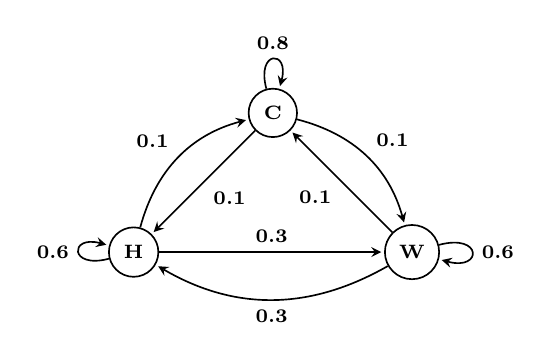
\begin{tikzpicture}[
	> = stealth, % arrow head style
	shorten > = 1pt, % don't touch arrow head to node
	auto,
	node distance = 2.5cm, % distance between nodes
	semithick, % line style
	font=\scriptsize\bfseries
	]
	
	\node[circle,draw] (qC) {C};
	\node[circle,draw] (qH) [below left of=qC] {H};
	\node[circle,draw] (qW) [below right of=qC] {W};
	
	\path[->] 	
	(qC) 	edge [loop above] node {0.8} ()
			edge [] node {0.1} (qH)
			edge [bend left] node {0.1} (qW)
	(qH) 	edge [loop left] node {0.6} ()
			edge [bend left] node {0.1} (qC)
			edge [] node {0.3} (qW)
	(qW)	edge [loop right] node {0.6} ()
			edge [bend left] node {0.3} (qH)
			edge [] node {0.1} (qC);
	\end{tikzpicture}
	\caption[Exemple d'un chaîne de Markov pour la prédiction du temps.]{Exemple d'un chaîne de Markov pour la prédiction du temps ; figure reconstruite de \cite{2019-jurafsky-martin}.}
	\label{fig:cm-exp}
\end{figure}

%\begin{figure}[ht]
%	\centering
%	\hgraphpage[.4\textwidth]{exp-markov_.pdf}
%	\caption[Exemple d'un chaîne de Markov pour la prédiction du temps]{Exemple d'un chaîne de Markov pour la prédiction du temps \cite{2019-jurafsky-martin}\label{fig:cm-exp}}
%\end{figure}

Ceci est un modèle de langage qui ne représente que les probabilités de transition. 
Dans ce cas, nous pouvons seulement représenter la probabilité de transition d'une catégorie à une autre. 
Si nous estimions la probabilité d'émission d'un mot dans chaque état (étiquette), nous pourrions estimer les étiquettes en utilisant la  théorème de Bayes. 
Ce modèle est appelé : modèle de Markov caché (\keyword[H]{\ac{hmm}}) ; les mots d'une séquence sont observés contrairement aux catégories qui sont cachées et doivent être estimées. 
Chaque étiquette (catégorie) $t_i$ est représentée par un un état $q_i$ dans l'ensemble des états $Q = \{q_1, q_2, \ldots, q_n\}$.
Les transitions d'un état vers un autre suivant un modèle Bi-gramme sont représentées par la matrice de transitions $A$.
La distribution initiale des probabilités de ces états est annotée $\pi = [\pi_1, \pi_2, \ldots, \pi_n ]$ où $\sum_i \pi_i = 1$.
Un mot $w_i$ est représenté comme une observation dans la séquences des évènements observés $O = o_1 o_2 \ldots o_T$. 
Une observation $o_t$ peut être générée dans un état $q_i$ avec une probabilités d'observation (probabilités d'émission) $B = b_i(o_t)$.
Un exemple d'un \keyword[H]{\ac{hmm}} est illustré dans la figure \ref{fig:hmm-exp}. 
Les transitions représentent les probabilités de passer d'une étiquette à une autre.
Les missions représentent les probabilités d'occurrence des mots dans les étiquettes.
\begin{figure}[ht]
	\centering
	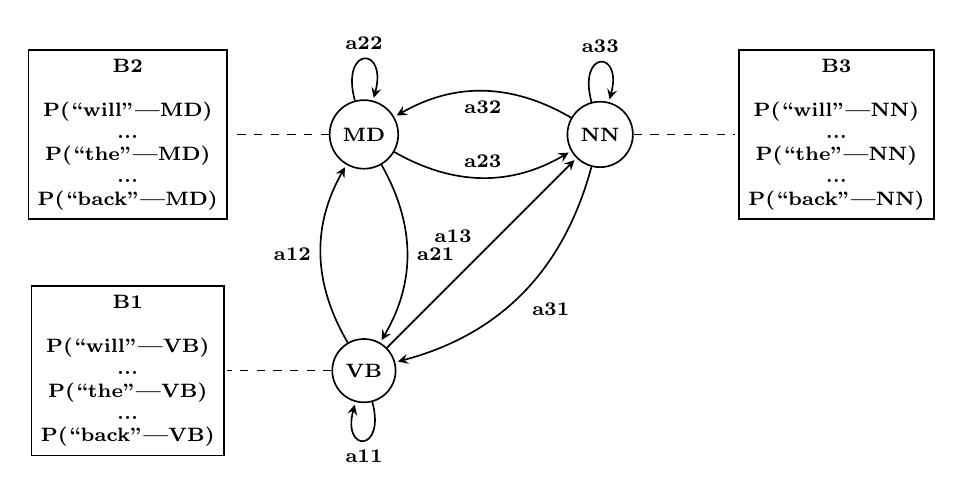
\begin{tikzpicture}[
	> = stealth, % arrow head style
	shorten > = 1pt, % don't touch arrow head to node
	auto,
	node distance = 3cm, % distance between nodes
	semithick, % line style
	font=\scriptsize\bfseries
	]
	
	\node[circle,draw] (q2) {MD};
	\node[align=center,draw] (q2e) [left of=q2] {B2\\ \\P(``will"|MD)\\...\\P(``the"|MD)\\...\\P(``back"|MD)};
	\node[circle,draw] (q3) [right of=q2] {NN};
	\node[align=center,draw] (q3e) [right of=q3] {B3\\ \\P(``will"|NN)\\...\\P(``the"|NN)\\...\\P(``back"|NN)};
	\node[circle,draw] (q1) [below of=q2] {VB};
	\node[align=center,draw] (q1e) [left of=q1] {B1\\ \\P(``will"|VB)\\...\\P(``the"|VB)\\...\\P(``back"|VB)};
	
	\path[->] 	
	(q1) 	edge [loop below] node {a11} ()
			edge [bend left] node {a12} (q2)
			edge [] node {a13} (q3)
	(q2) 	edge [loop above] node {a22} ()
			edge [bend left] node {a21} (q1)
			edge [bend right] node {a23} (q3)
	(q3)	edge [loop above] node {a33} ()
			edge [bend left] node {a31} (q1)
			edge [bend right] node {a32} (q2);
	
	\path[dashed] 	
	(q1) 	edge [] node {} (q1e)
	(q2) 	edge [] node {} (q2e)
	(q3) 	edge [] node {} (q3e);
	
	\end{tikzpicture}
	\caption[Exemple d'une représentation HMM]{Exemple d'une représentation HMM ; figure reconstruite de \cite{2019-jurafsky-martin}.}
	\label{fig:hmm-exp}
\end{figure}

%\begin{figure}[ht]
%	\centering
%	\hgraphpage[.6\textwidth]{exp-hmm_.pdf}
%	\caption[Exemple d'une représentation HMM]{Exemple d'une représentation HMM \cite{2019-jurafsky-martin}\label{fig:hmm-exp}}
%\end{figure}

La séquence estimée $\hat{t}$ est celle qui maximise la probabilité $P(t)$ et la probabilité $P(w | t)$ selon l'équation \ref{eq:hmm-detail}.
En utilisant un modèle \keyword[B]{Bi-gramme}, la probabilité $P(t)$ est calculée en utilisant les transitions de l'état initial $t_1$ jusqu'à le dernier $t_n$. 
Il faut savoir que la probabilité $P(t_1|t_0)$ est en réalité la probabilité initiale $\pi_1$ de l'état $t_1$.
La probabilité $P(w_i | t_i)$ est une probabilité d'émission dans le modèle de Markov caché.
\begin{align}
\hat{t} & = \arg\max\limits_t P(t) P(w | t) \nonumber\\
		& = \arg\max\limits_t P(t_1 \dots t_n) P(w_1 \dots w_n | t_1 \dots t_n) \nonumber\\
		& = \arg\max\limits_t \pi_{t1} \prod_{i=2}^{n} P(t_i|t_{i-1}) \prod_{i=1}^{n} P(w_i| t_i) \nonumber\\
        & = \arg\max\limits_t \prod_{i=1}^{n} \underbrace{P(t_i|t_{i-1})}_{a_{i-1,i}} \underbrace{P(w_i | t_i)}_{b_i(w_i)} \label{eq:hmm-detail}
\end{align}

Avant de discuter comment une séquence $w=w_1 \ldots w_n$ est décodée selon l'équation \ref{eq:hmm-detail}, nous commençons par décrire l'entraînement. 
Dans un \keyword[H]{\ac{hmm}}, les états sont les tags (catégories) $t_i$ et les observations sont les mots $w_i$. 
Notons la fonction qui compte le nombre des occurrence d'une séquence comme $C$.
La probabilité de transition $a_{i-1,i}$ de l'état $t_{i-1}$ vers $t_i$ est estimée à partir du corpus d'entraînement selon l'équation \ref{eq:pos-hmm1}.
Notons ``<s>" ; l'étiquette qui précède la première catégorie de la phrase. 
Dans ce cas, la probabilité $\pi_i$ de commencer par l'état $t_i$ est estimée selon l'équation \ref{eq:pos-hmm2}.
La probabilité d'émission d'un mot $w_i$ dans un état $t_i$ est estimée selon l'équation \ref{eq:pos-hmm3}.
\begin{align}
P(t_i | t_{i-1}) = \frac{C(t_{i-1}, t_i)}{C(t_{i-1})}  \label{eq:pos-hmm1} \\
\pi_i = P(t_i | <s>) = \frac{C(<s>, t_i)}{C(<s>)} \label{eq:pos-hmm2} \\
P(w_i | t_i) = \frac{C(t_i, w_i)}{C(t_i)} \label{eq:pos-hmm3}
\end{align}

Prenons un exemple d'un corpus d'entraînement avec quatre phrases. 
Nous avons 4 catégories : DT, PR, VB et NM. 
\begin{itemize}
	\item un/DT ordinateur/NM peut/VB vous/PR aider/VB
	\item il/PR veut/VB vous/PR aider/VB
	\item il/PR veut/VB un/DT ordinateur/NM
	\item il/PR peut/VB nager/VB  
\end{itemize}
Un exemple de calcul d'une transition est le suivant : $P(VB | NM) = \frac{C(NM,\ VB)}{C(NM)} = \frac{1}{2}$. 
La probabilité d'émission du mot ``veut" lorsque le tag est ``VB" est calculée comme suit : $P(veut | VB) = \frac{C(VB,\ veut)}{C(VB)} = \frac{2}{7}$. 
La probabilité q'un pronom soit au début de la phrase est calculée comme : $\pi_{PR} = \frac{C(<s>,\ PR)}{C(<s>)} = \frac{3}{4} $.
La matrice des transitions ainsi que la distribution initiale sont illustrés dans le tableau \ref{tab:hmm-trans-init}. 
Pourtant ce n'est pas utilisé dans le calcul, nous avons ajouté le passage d'un état vers la fin afin de compléter la distribution (avoir une somme de 1 sur les lignes). 
Les probabilités d'émission sont illustrées dans le tableau \ref{tab:hmm-emission}. 
\begin{table}[ht]
	\centering\footnotesize
\begin{tabular}{llllll}
	\cline{2-6}\noalign{\vskip\doublerulesep
		\vskip-\arrayrulewidth}\cline{2-6}
	     & DT & PR & VB & NM & \textless/s\textgreater\\
	\hline
	DT  &  0  &  0   &  0   &   1  &  0  \\
	PR &  0  &  0   &   1  &  0   &  0  \\
	VB & 1/7 & 2/7  & 1/7  &  0   & 3/7 \\
	NM &  0  &  0   & 1/2  &   0  &  1/2 \\
	\hline
	\textless s\textgreater ($\pi$) &  1/4  &  3/4   & 0  &   0  &  0 \\
	\hline\hline
\end{tabular}
\caption[Exemple des probabilités de transition et une distribution initiale]{Exemple des probabilités de transition et une distribution initiale \label{tab:hmm-trans-init}}
\end{table}

\begin{table}[ht]
	\centering\footnotesize
\begin{tabular}{lllllllll}
	\cline{2-9}\noalign{\vskip\doublerulesep
		\vskip-\arrayrulewidth}\cline{2-9}
	     & un & ordinateur & peut & vous & aider & il & veut & nager \\
	\hline
	DT  &  1 &  0         &  0   &   0  &  0    & 0  & 0    & 0 \\
	PR &  0 &  0         &  0   & 1/4  &  0    &3/4 & 0    & 0 \\
	VB &  0 &  0         & 2/7  &   0  &  2/7  & 0  & 2/7  & 1/7 \\
	NM &  0 &  1         &  0   &   0  &  0    & 0  & 0    & 0 \\
	\hline\hline
\end{tabular}
\caption[Exemple des probabilités d'émission]{Exemple des probabilités d'émission \label{tab:hmm-emission}}
\end{table}

%\begin{figure}
%	\begin{tikzpicture}[
%	> = stealth, % arrow head style
%	shorten > = 1pt, % don't touch arrow head to node
%	auto,
%	node distance = 3cm, % distance between nodes
%	semithick, % line style
%	font=\small
%	]
%	
%	\tikzstyle{every state}=[
%	draw = black,
%	thick,
%	fill = white,
%	minimum size = 4mm
%	]
%	
%	\node[circle,draw] (qN) {N};
%	\node[align=left,draw] (qNe) [left of=qN] {P("fish"|N)=0.05\\P("river"|N)=0.03};
%	\node[circle,draw] (qV) [right of=qN] {V};
%	\node[align=left,draw] (qVe) [right of=qV] {P("fish"|V)=0.01\\P("eat"|V)=0.02};
%	\node[circle,draw] (qD) [below of=qN] {D};
%	\node[align=left,draw] (qDe) [left of=qD] {P("the"|D)=0.3\\P("a"|D)=0.2\\P("an"|D)=0.15};
%	\node[circle,draw] (qP) [right of=qD] {P};
%	\node[align=left,draw] (qPe) [right of=qP] {P("I"|P)=0.2\\P("he"|P)=0.1\\P("she"|P)=0.1};
%	\node[] () [below of=qD, yshift=1.5cm] {$\pi(P, D, V, N) = (0.4, 0.3, 0.1, 0.2)$};
%	
%	
%	\path[->] 	
%	(qN) 	edge [loop above] node {0.3} ()
%	edge [bend left] node {0.7} (qV)
%	(qV) 	edge [loop above] node {0.1} ()
%	edge [bend left] node {0.5} (qN)
%	edge [bend left] node {0.4} (qD)
%	(qD)	edge [bend left] node {1.0} (qN)
%	(qP)	edge [bend right] node {1.0} (qV);
%	
%	\path[dashed] 	
%	(qN) 	edge [] node {} (qNe)
%	(qV) 	edge [] node {} (qVe)
%	(qD) 	edge [] node {} (qDe)
%	(qP) 	edge [] node {} (qPe);
%	
%	\end{tikzpicture}
%	\caption{Exemple}
%\end{figure}

Revenons maintenant au décodage des tags (étiquetage). 
Après l'entraînement d'un modèle de Markov caché $\lambda = (A, B)$, nous voulons l'utiliser pour estimer la séquence des étiquettes $\hat{t} = \hat{t}_1 \hat{t}_2 \ldots \hat{t}_T$ à partir d'une séquence des observations (mots) $w = w_1 w_2 \ldots w_T$ où nous possédons $N$ tags possibles.
Si nous utilisions un décodage par force brute, nous aurions une complexité de $O(N^T)$.
Vu que la maximisation des tags d'une observation (mot) $w_t$ ne dépend que sur les tags de l'observation précédente, nous pouvons résoudre le problème de la recherche en utilisant la programmation dynamique.
Dans chaque étape $t$ de la séquence, nous nous basons sur l'estimation précédente pour calculer les probabilités de tous les tags afin de choisir celui qui maximise la probabilité comme estimation courante. 
Il faut toujours sauvegarder l'état précédent pour revenir en fin d'algorithme. 
Ceci est appelé la recherche \keyword[V]{Viterbi} (voir l'algorithme \ref{algo:viterbi}).
Dans ce cas, la complexité est réduite à $O(N^2T)$ et la recherche reste toujours exacte.

\begin{algorithm}[ht]
	\KwData{$w = w_1 \ldots w_T$, HMM $\lambda = (A, B)$ avec $N$ états}
	\KwResult{$meilleur\_chemin$, $prob\_chemin$}
	
	Créer deux matrices $viterbi[N, T]$ et $backpointer[N, T]$\;
	
	\Pour{état $ s = 1 \ldots N$}{
		$viterbi[s, 1] = \pi_s * b_s(w_1);\, backpointer[s, 1] = 0$ \;
	}
	
	\Pour{$ t = 2 \ldots T$}{
		\Pour{état $ s = 1 \ldots N$}{
			$viterbi[s, t] = \max\limits_{s'=1}^N viterbi[s', t-1] * a_{s',s} * b_s(w_t)$\;
			$backpointer[s, t] = \arg\max\limits_{s'=1}^N viterbi[s', t-1] * a_{s',s} * b_s(w_t)$\;
		}
	}
	
	$prob\_chemin = \max\limits_{s=1}^N viterbi[s, T];\, pointeur\_chemin = \arg\max\limits_{s=1}^N viterbi[s, T]$\;
	
	$meilleur\_chemin$ est le chemin qui commence par $pointeur\_chemin$ et qui suit $backpointer$
	
	\Return $meilleur\_chemin$, $prob\_chemin$\;
	\caption{Algorithme de Viterbi pour encoder une séquence selon un modèle de Markov caché.}
	\label{algo:viterbi}
\end{algorithm}

En utilisant le modèle entraîné dans l'exemple précédent, nous voulons trouver les tags de cette phrase : \expword{il peut aider}. 
Suivant l'algorithme de Viterbi, nous aurons le tableau \ref{tab:hmm-viterbi-exp} où chaque cellule est remplie par les calculs séparés par des points virgules (les états précédent) et le pointeur de retour entre deux crochets. 
Dans la dernière séquence (``aider"), l'état qui maximise la probabilité est ``VB". 
Le retour est l'état 3 (``VB") ayant un retour vers l'état 2 (``PR"). 
Donc, le texte annoté est : \expword{il/PR peut/VB aider/VB}. 

%\begin{table}[ht]
%	\centering\small
%	\begin{tabular}{llll}
%		\cline{2-4}\noalign{\vskip\doublerulesep
%			\vskip-\arrayrulewidth}\cline{2-4}
%		       & il & peut & aider \\
%		\hline
%		\multirow{4}{*}{DET}  &  \multirow{4}{*}{1/4 * 0}& 0 * 0 * 0 & 0 * 0 * 0 \\
%		  &  & 3/4 * 0 * 0 & 0 * 0 * 0\\
%		  &  & 0 * 1/7 * 0 & 6/28 * 1/7 * 0 \\
%		  &  & 0 * 0 * 0 & 0 * 0 * 0\\
%		\multirow{4}{*}{PRON} &  \multirow{4}{*}{3/4 * 1} &  0 * 0 * 0&  0 * 0 * 0\\
%		  &  & 3/4 * 0 * 0 & 0 * 0 * 0\\
%		  &  & 0 * 2/7 * 0 & 6/28 * 2/7 * 0\\
%		  &  & 0 * 0 * 0 & 0 * 0 * 0 \\
%		\multirow{4}{*}{VERB} &  \multirow{4}{*}{0 * 0} & 0 * 0 * 2/7 & 0 * 0 * 2/7 \\
%		  &  & 3/4 * 1 * 2/7 & 0 * 1 * 2/7 \\
%		  &  & 0 * 1/7 * 2/7 & 6/28 * 1/7 * 2/7\\
%		  &  & 0 * 1/2 * 2/7 & 0 * 1/7 * 2/7 \\
%		\multirow{4}{*}{NOUN} &  \multirow{4}{*}{0 * 0} & 0 * 1 * 0 & 0 * 1 * 0 \\
%		  &  & 3/4 * 0 * 0 & 6/28 * 0 * 0 \\
%		  &  & 0 * 0 * 0 & 0 * 0 * 0 \\
%		  &  & 0 * 0 * 0 & 0 * 0 * 0\\
%		\hline\hline
%	\end{tabular}
%	\caption{Un exemple des probabilités d'émission \label{tab:hmm-viterbi-exp}}
%\end{table}

\begin{table}[ht]
	\centering\footnotesize%\scriptsize
	\begin{tabular}{llll}
		\cline{2-4}\noalign{\vskip\doublerulesep
			\vskip-\arrayrulewidth}\cline{2-4}
		& il & peut & aider \\
		\hline
		DT  & $\frac{1}{4} * 0$ [0]& $0 * 0 * 0$; $\frac{3}{4} * 0 * 0$; $0 * \frac{1}{7} * 0$; $0 * 0 * 0$ [2] & $0 * 0 * 0$; $0 * 0 * 0$; $\frac{6}{28} * \frac{1}{7} * 0$; $0 * 0 * 0$ [3]\\
		PR & $\frac{3}{4} * 1$ [0]&  $0 * 0 * 0$; $\frac{3}{4} * 0 * 0$; $0 * \frac{2}{7} * 0$; $0 * 0 * 0$ [2]&  $0 * 0 * 0$; $0 * 0 * 0$; $\frac{6}{28} * \frac{2}{7} * 0$; $0 * 0 * 0$ [3]\\
		VB & $0 * 0$ [0]& $0 * 0 * \frac{2}{7}$; $\frac{3}{4} * 1 * \frac{2}{7}$; $0 * \frac{1}{7} * \frac{2}{7}$; $0 * \frac{1}{2} * \frac{2}{7}$ [2]& $0 * 0 * \frac{2}{7}$; $0 * 1 * \frac{2}{7}$; $\frac{6}{28} * \frac{1}{7} * \frac{2}{7}$; $0 * \frac{1}{7} * \frac{2}{7}$ [3]\\
		NM & $0 * 0$ [0]& $0 * 1 * 0$; $\frac{3}{4} * 0 * 0$; $0 * 0 * 0$; $0 * 0 * 0$ [1]& $0 * 1 * 0$; $\frac{6}{28} * 0 * 0$; $0 * 0 * 0$; $0 * 0 * 0$ [1]\\
		\hline\hline
	\end{tabular}
	\caption[Exemple d'exécution de l'algorithme de Viterbi]{Exemple d'exécution de l'algorithme de Viterbi \label{tab:hmm-viterbi-exp}}
\end{table}


\subsection{Maximum entropy}

Les estimations par \keyword[H]{\ac{hmm}} se basent seulement sur des statistiques des mots. 
Il est difficile d'introduire des caractéristiques comme les suffixes, le majuscule, etc. 
La régression logistique, qui est un modèle discriminatif, peut combiner plusieurs caractéristiques afin d'estimer une probabilité de sortie. 
Malheureusement, cette méthode ne prend pas les séquences en considération.
Nous pouvons utiliser des caractéristiques sur le mot actuel et les mots avant afin d'estimer l'étiquette ; comme dans les \keyword[H]{\ac{hmm}}.
Dans ce cas le modèle sera appelé \acf{memm}.
Le problème revient à maximiser les probabilités individuelles de chaque étiquette $\hat{t}_i$ (voir l'équation \ref{eq:pos-emm-est}). 
\begin{equation}\label{eq:pos-emm-est}
\hat{t} = \arg\max\limits_t P(t | w) = \arg\max\limits_t \prod\limits_{i}  P(t_i | w_i, t_{i-1})
\end{equation}
Notons $s_i^j$ la séquence $s_i \ldots s_j$. 
Afin d'estimer l'étiquette $t_i$ d'un mot $w_i$, nous prenons $l$ mots précédents et $l$ mots suivants, en plus de $k$ tags précédents.
Nous utilisons un ensemble des caractéristiques $f$ où $f_j$ peut être la présence du majuscule dans le mot, etc.
En utilisant la régression logistique, le problème sera formulé comme dans l'équation \ref{eq:memm}.
L'apprentissage vise à minimiser la somme des erreurs d'étiquetage multi-classes de chaque mot (pour chaque mot, nous aurons plusieurs probabilités ; une pour chaque étiquette).
\begin{equation}\label{eq:memm}
\hat{t} = \arg\max\limits_t \prod\limits_{i}  
\frac{exp\left(\sum_j \theta_j f_j(t_i, w_{i-l}^{i+l}, t_{i-k}^{i-1})\right)}%
{\sum_{t' \in tags} exp\left(\sum_j \theta_j f_j(t'_i, w_{i-l}^{i+l}, t_{i-k}^{i-1})\right)}
\end{equation}

Voici une liste des caractéristiques $f$ que nous pouvons utiliser dans cette méthode :
\begin{itemize}
	\item Le mot $w_i$ (en considérant chaque mot comme caractéristique)
	\item Les étiquettes précédentes 
	\item $w_i$ contient un préfixe à partir d'une liste (\textit{len(prefixe)} $\le 4$) 
	\item $w_i$ contient un suffixe à partir d'une liste (\textit{len(suffixe)} $\le 4$) 
	\item $w_i$ contient un nombre 
	\item $w_i$ contient une lettre en majuscule
	\item $w_i$ contient un trait d'union 
	\item $w_i$ est complètement en majuscule
	\item La forme du mot $w_i$ (Ex. \expword{X.X.X}) 
	\item $w_i$ est en majuscule avec un trait et un nombre (Ex. \expword{CFC-12}) 
	\item $w_i$ est en majuscule suivi des mots Co., Inc., etc. dans 3 mots maximum
\end{itemize}

\subsection{Modèle neuronal}

Les réseaux de neurones récurrents sont conçus pour traiter les séquences.
Nous avons vu qu'un \ac{rnn} peut être utilisé comme modèle de langage en passant le mot encodé avec \keyword[O]{One-Hot} en entrée et en estimant le mot suivant sachant le contexte précédent. 
Nous modifions la sortie : à la place des probabilités des mots du vocabulaire, nous essayons d'estimer les probabilités des catégories possibles. 
Nous pouvons, bien sûr, utiliser une couche cachée pour apprendre une représentation plus compacte des mots en entrée (\keyword[E]{embedding}). 
La figure \ref{fig:pos-rnn1} représente un exemple d'un réseau de neurones récurrent pour la détection des étiquettes morpho-syntaxique suivant cette modification.
\begin{figure}[ht]
	\centering
	\hgraphpage[.6\textwidth]{rnn-simple.pdf}
	\caption[RNN simple pour l'étiquetage morpho-syntaxique.]{RNN simple pour l'étiquetage morpho-syntaxique.}
	\label{fig:pos-rnn1}
\end{figure}
%\begin{figure}[!ht]
%	\centering
%	\hgraphpage[.55\textwidth]{rnn-simple_.pdf}
%	\caption[RNN simple pour l'étiquetage morpho-syntaxique]{RNN simple pour l'étiquetage morpho-syntaxique \cite{2019-jurafsky-martin}\label{fig:pos-rnn1}}
%\end{figure}

Si nous voulions avoir des réseaux plus profonds et plus complexes, nous pourrions empiler plusieurs \ac{rnn} ensembles. 
Cela permet au modèle d'apprendre des traitements plus complexes améliorant la prédiction.
Pour entraîner ce modèle, nous aurons besoin d'un grand dataset ; la taille de ce dernier augmente avec le nombre des réseaux empilés.
La figure \ref{fig:pos-rnn2} est une illustration d'un modèle avec deux \ac{rnn} empilés.
\begin{figure}[ht]
	\centering
	\hgraphpage[.7\textwidth]{rnn-stack.pdf}
	\caption[RNNs empilés pour l'étiquetage morpho-syntaxique.]{RNNs empilés pour l'étiquetage morpho-syntaxique.}
	\label{fig:pos-rnn2}
\end{figure}
%\begin{figure}[!ht]
%	\centering
%	\hgraphpage[.55\textwidth]{rnn-stack_.pdf}
%	\caption[RNNs empilés pour l'étiquetage morpho-syntaxique]{RNNs empilés pour l'étiquetage morpho-syntaxique \cite{2019-jurafsky-martin}\label{fig:pos-rnn2}}
%\end{figure}

Dans les modèles neuronaux précédents, l'étiquette courante $t_i$ dépend sur le mot courant $w_i$ et le contexte passé. 
Des fois, savoir le contexte futur peut améliorer la décision courante ; nous pouvons trouver une dépendance entre le mot courant et les mots après. 
Afin d'estimer l'étiquette courante en se basant sur le contexte futur, nous utilisons un \ac{rnn} avec une séquence inversée ; c-à-d. l'étiquette $t_i$ sera dépendante à la séquence $w_n, w_{n-1}, \ldots, w_{i+1}, w_{i}$. 
Afin d'exprimer la bidirectionnalité, nous utilisons deux \ac{rnn} : en avant $RNN_{forward}(w_1^i)$ et en arrière $RNN_{backword}(w_i^n)$. 
Nous calculons la somme entre les deux états cachés $h_i^f \oplus h_i^b$ résultant à un vecteur qui doit passer par une fonction ``softmax" afin d'estimer les probabilités des tags. 
Cette architecture est illustrée dans la figure \ref{fig:pos-rnn3}.
\begin{figure}[ht]
	\centering
	\hgraphpage[.7\textwidth]{rnn-bi.pdf}
	\caption[RNN bidirectionnel pour l'étiquetage morpho-syntaxique.]{RNN bidirectionnel pour l'étiquetage.}
	\label{fig:pos-rnn3}
\end{figure}
%\begin{figure}[!ht]
%	\centering
%	\hgraphpage[.60\textwidth]{rnn-bi_.pdf}
%	\caption[RNN bidirectionnel pour l'étiquetage morpho-syntaxique]{RNN bidirectionnel pour l'étiquetage morpho-syntaxique \cite{2019-jurafsky-martin}\label{fig:pos-rnn3}}
%\end{figure}

Les langues sont toujours en amélioration : ajout des nouveaux mots, des nouvelles formes, etc. 
En plus, nous ne pouvons pas capturer toutes les variations de tous les mots en utilisant un corpus limité surtout dans les langues fortement flexionnelles. 
Afin de représenter les variations morphologiques d'un mot, nous devons descendre au niveau caractère.
Une idée (voir la figure \ref{fig:pos-rnn4}) est d'utiliser un modèle de langage au niveau caractère afin d'encoder un mot et combiner ce code avec le code lexicale (\keyword[O]{One-Hot} ou \keyword[E]{embedding}) du mot. 
Le code résultat sera pris comme l'entrée du réseau récurrent (simple, empilé ou bidirectionnel).
\begin{figure}[ht]
	\centering
	\hgraphpage[0.8\textwidth]{rnn-char.pdf}
	\caption[Embedding de caractères pour l'étiquetage morpho-syntaxique.]{RNN avec des embedding de caractères pour l'étiquetage morpho-syntaxique.}
	\label{fig:pos-rnn4}
\end{figure}
%\begin{figure}[ht]
%	\centering
%	\hgraphpage[0.5\textwidth]{rnn-char1_.pdf}
%	\hgraphpage[0.45\textwidth]{rnn-char2_.pdf}
%	\caption[Embedding de caractères pour l'étiquetage morpho-syntaxique]{RNN avec des embedding de caractères pour l'étiquetage morpho-syntaxique \cite{2019-jurafsky-martin}\label{fig:pos-rnn4}}
%\end{figure}

\sectioni{Discussion}
%\begin{discussion}
Chaque langue doit avoir un mécanisme pour identifier les entités existantes dans le monde (plantes, animaux, villes, etc.) et les actions qu'une entité puisse exécuter (Ex. jouer, lire, exister, etc.). 
Les linguistes font la différence entre la fonction d'un mot dans la phrase en utilisant des catégories. 
Par exemple un nom c'est la référence à un objet (concret ou abstrait), or un adjectif est un mot qui représente une propriété d'un nom. 
Donc, le fait de savoir la catégorie d'un mot aide la compréhension d'une phrase. 
Automatiser la tâche de détection des catégories d'une séquence de mots est une étape vers la compréhension de la phrase. 
Même dans les tâches statistiques (qui n'ont pas besoin de la compréhension), les catégories des mots peuvent être un bon indicateur. 

Étiqueter les mots par leurs catégories grammaticales est une tâche appartenant aux tâches de l'étiquetage des séquences. 
Plusieurs approches ont été utilisées pour résoudre ce problème : par règles, statistique et par réseaux de neurones. 
Les règles sont difficiles à mettre en œuvre ; il faut avoir une connaissance profonde de la langue traitée.
Cette approche a été remplacée par l'approche statistique qui vise à estimer l'étiquette en se basant sur des statistiques sur le mot actuel ainsi que les mots précédents et leurs étiquettes.
Avec l'arrivée des \ac{rnn}, cette tâche a devenue plus facile ; il faut juste avoir un corpus étiqueté avec une taille suffisante. 
Dans les architectures présentées dans ce chapitre, l'entrée d'un \ac{rnn} est une représentation vectorielle du mot courant. 
En réalité, nous pouvons définir des architectures plus complexes en introduisant les caractéristiques d'un mot comme par exemple la présence des suffixes. 
Nous pouvons même encoder tous les suffixes avec l'encodage One-Hot et fusionner ce code avec celui du mot. 

Dans ce chapitre, nous avons présenté l'étiquetage des séquences et plus précisément l'étiquetage morpho-syntaxique. 
Nous avons vu les approches et quelques méthodes utilisées pour résoudre cette tâche. 
Mais la question qui se pose : comment pouvons-nous évaluer un système d'étiquetage des séquences ? 
Tout simplement, cette tâche est un cas spécial de classification : à la place de classer une phrase, nous classons chaque mot (ou partie) à part en tenant compte de leurs interactions (temporelles). 
Donc, les métriques d'évaluation de la classification comme la justesse (accuracy), le rappel (recall), la précision (precision), etc. peuvent être utilisées.
Cela concerne l'évaluation intrinsèque, sinon nous pouvons évaluer l'effet de cette tâche sur une autre (évaluation extrinsèque).
%\end{discussion}

\sectioni{Ressources supplémentaires}
%\begin{ressources}

\subsubsection*{Exercices}

\begin{enumerate}
	\item Voici un modèle de Markov caché pour l'étiquetage morpho-syntaxique : 
	
	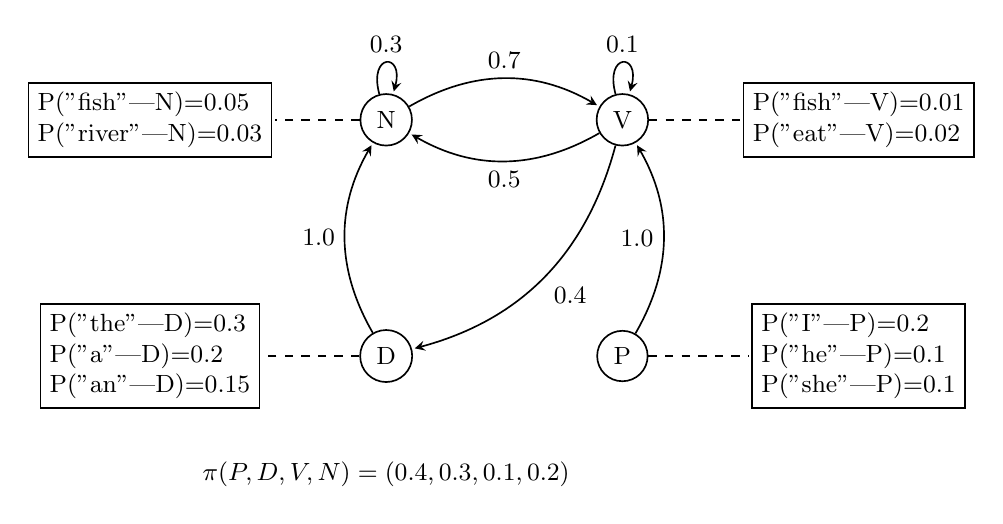
\begin{tikzpicture}[
	> = stealth, % arrow head style
	shorten > = 1pt, % don't touch arrow head to node
	auto,
	node distance = 3cm, % distance between nodes
	semithick, % line style
	font=\small
	]
	
	\tikzstyle{every state}=[
	draw = black,
	thick,
	fill = white,
	minimum size = 4mm
	]
	
	\node[circle,draw] (qN) {N};
	\node[align=left,draw] (qNe) [left of=qN] {P("fish"|N)=0.05\\P("river"|N)=0.03};
	\node[circle,draw] (qV) [right of=qN] {V};
	\node[align=left,draw] (qVe) [right of=qV] {P("fish"|V)=0.01\\P("eat"|V)=0.02};
	\node[circle,draw] (qD) [below of=qN] {D};
	\node[align=left,draw] (qDe) [left of=qD] {P("the"|D)=0.3\\P("a"|D)=0.2\\P("an"|D)=0.15};
	\node[circle,draw] (qP) [right of=qD] {P};
	\node[align=left,draw] (qPe) [right of=qP] {P("I"|P)=0.2\\P("he"|P)=0.1\\P("she"|P)=0.1};
	\node[] () [below of=qD, yshift=1.5cm] {$\pi(P, D, V, N) = (0.4, 0.3, 0.1, 0.2)$};
	
	
	\path[->] 	
	(qN) 	edge [loop above] node {0.3} ()
	edge [bend left] node {0.7} (qV)
	(qV) 	edge [loop above] node {0.1} ()
	edge [bend left] node {0.5} (qN)
	edge [bend left] node {0.4} (qD)
	(qD)	edge [bend left] node {1.0} (qN)
	(qP)	edge [bend right] node {1.0} (qV);
	
	\path[dashed] 	
	(qN) 	edge [] node {} (qNe)
	(qV) 	edge [] node {} (qVe)
	(qD) 	edge [] node {} (qDe)
	(qP) 	edge [] node {} (qPe);
	
	\end{tikzpicture}
	
	\begin{enumerate}
		\item Calculer les deux probabilités : P(V D N | ``fish a fish") et P(N D N | "fish a fish")
		\item Étant donné que C(N) = 200, C(V) = 100 et C(D)=100, calculer les probabilités suivantes en utilisant le lissage de Laplace : P(D|V), P(D|N) et P(N|D).
		\item Recalculer les probabilités de la première question après le lissage.
		\item Combien d'expressions étiquetées ``\textbf{V D N}" existent-elles dans notre dataset d'entraînement ? Le déterminant ``\textbf{D}" ne se produit jamais à la fin de la phrase. 
		
	\end{enumerate}
	
\end{enumerate}

\subsubsection*{Tutoriels}

Les tutoriels sont accessibles via le répertoire Github.
Dans le premier tutoriel, nous présentons la tâche d'étiquetage morpho-syntaxique avec NLTK qui est un outil implémenté en python destiné pour TALN.
Plusieurs algorithmes sont utilisés : RegEx, CRF, HMM, Perceptron et Brill.
Nous présentons, aussi, la tâche d'extraction des entités nommées et celle d'extraction des syntagmes nominaux.

Le deuxième tutoriel utilise flair ; un outil en python pour TALN.
Nous présentons les deux tâches : étiquetage morphosyntaxique et extraction des entités nommées.
Dans le tutoriel, nous pouvons apprendre comment utiliser un modèle existant et comment créer un nouveau modèle.

\subsubsection*{TP : Analyse morphosyntaxique}

On veut concevoir un petit programme pour l'analyse morphosyntaxique à partir de zéro. 
Le modèle HMM avec lissage de Laplace est fourni.
L'étudiant doit implémenter la méthode de décodage ``viterbi".

L'énoncé complet du TP ainsi que les codes et les données sont téléchargeables à partir du répertoire Github.
Le TP est implémenté complètement à partir de zéro (from scratch) : le module HMM et le module qui l'utilise pour l'analyse morphosyntaxique. 
L'étudiant doit compléter deux fonctions du premier module : notation ($p(t_i|t_{i-1}, w_i)$) et décodage viterbi.
Deux autres algorithmes de décodage sont implémentés : force brute et gourmand.
L'étudiant doit comparer entre les trois modèles en calculant la complexité en temps.
Les langages de programmation disponibles (pour l'instant) sont : Java, Javascript/nodejs et Python.

%\subsubsection*{Lab}
%
%Dans la tâche du "Jugements d'acceptabilité", on essaye de deviner si une phrase est acceptable grammaticalement. 
%Par exemple, l'expression "\textbf{Le livre qu'ont puisse trouvé sur internet ...}" ne peut pas être considérée comme acceptable. 
%La raison est que le verbe "ont (avoir)" est moins probable de suivre "que" et que le verbe "puisse (pouvoir)" est conjugué en présent subjonctif, or il est plus probable d'être en infinitif s'il suit le verbe "avoir".
%Dans ce lab, on va essayé de tester des différents modèles de langages afin d'accomplir cette tâche.
%
%L'énoncé complet du lab est téléchargeable à partir du répertoire Github.
%Les outils utilisés sont NLTK et Keras.

%=====================================================================
\ifx\wholebook\relax\else
% \cleardoublepage
% \bibliographystyle{../use/ESIbib}
% \bibliography{../bib/RATstat}
	\end{document}
\fi
%=====================================================================


% !TEX TS-program = xelatex
% !TeX program = xelatex
% !TEX encoding = UTF-8
% !TeX spellcheck = fr

%=====================================================================
\ifx\wholebook\relax\else
	\documentclass{KodeBook}
	
\bibliographystyle{unsrtnat}%unsrtnat, plainnat

\hypersetup{
	pdfkeywords={NLP; Language},
	pdfsubject={Artificial intelligence; Natural Language Processing},
	citecolor=blue,
}



\DeclareAcronym{amr}{
	short = AMR,
	long  =  Abstract Meaning Representation,
	tag = abbrev
}

\DeclareAcronym{cfg}{
	short = CFG ,
	long  =  Context Free Grammar,
	tag = abbrev
}

\DeclareAcronym{darpa}{
	short = DARPA ,
	long  = Defense Advanced Research Projects Agency,
	tag = abbrev
}

\DeclareAcronym{edu}{
	short = EDU,
	long  = Elementary Discourse Unit,
	tag = abbrev
}

\DeclareAcronym{fol}{
	short = FOL,
	long  = First Order Logic,
	tag = abbrev
}

\DeclareAcronym{hmm}{
	short = HMM ,
	long  =  Hidden Markov Model,
	tag = abbrev
}

\DeclareAcronym{ia}{
	short = IA ,
	long  = Intelligence Artificielle,
	tag = abbrev
}

\DeclareAcronym{ibm}{
	short = IBM,
	long  = International Business Machines,
	tag = abbrev
}

\DeclareAcronym{idf}{
	short = IDF ,
	long  = Inverse Document Frequency,
	tag = abbrev
}

\DeclareAcronym{ipa}{
	short = IPA ,
	long  = Intelligent Personal Assistant,
	tag = abbrev
}

\DeclareAcronym{iva}{
	short = IVA ,
	long  = Intelligent Virtual Assistant,
	tag = abbrev
}

\DeclareAcronym{ipa2}{
	short = IPA ,
	long  =  International Phonetic Alphabet,
	tag = abbrev
}

\DeclareAcronym{lsa}{
	short = LSA,
	long  = Latent Semantic Analysis,
	tag = abbrev
}

\DeclareAcronym{memm}{
	short = MEMM ,
	long  =  Maximum Entropy Markov Model,
	tag = abbrev
}

\DeclareAcronym{ml}{
	short = ML,
	long  = Machine Learning,
	tag = abbrev
}

\DeclareAcronym{pcfg}{
	short = PCFG ,
	long  = Probabilistic Context Free Grammar,
	tag = abbrev
}

\DeclareAcronym{pdtb}{
	short = PDTB,
	long  = Penn Discourse TreeBank,
	tag = abbrev
}

\DeclareAcronym{ri}{
	short = RI,
	long  =  Recherche d'Information,
	tag = abbrev
}

\DeclareAcronym{rnn}{
	short = RNN ,
	long  = Recurrent Neural Network,
	tag = abbrev
}

\DeclareAcronym{rst}{
	short = RST,
	long  = Rhetorical Structure Theory,
	tag = abbrev
}

\DeclareAcronym{srl}{
	short = SRL,
	long  = Semantic Role Labeling,
	tag = abbrev
}

\DeclareAcronym{svd}{
	short = SVD,
	long  = Singular Value Decomposition,
	tag = abbrev
}


\DeclareAcronym{taln}{
	short = TALN,
	long  = Traitement Automatique du Langage Naturel,
	tag = abbrev
}

\DeclareAcronym{tal}{
	short = TAL ,
	long  = Traitement Automatique des Langues,
	tag = abbrev
}

\DeclareAcronym{tf}{
	short = TF ,
	long  = Term Frequency,
	tag = abbrev
}

\DeclareAcronym{tfidf}{
	short = TF-IDF ,
	long  = Term Frequency - Inverse Document Frequency,
	tag = abbrev
}

\DeclareAcronym{wsd}{
	short = WSD ,
	long  = Word Sense Disambiguation,
	tag = abbrev
}


%\makeglossaries

%\newacronym{oop}{OOP}{Object-oriented programming} 

	\begin{document}
		\mainmatter
	
\fi
%=====================================================================
\changegraphpath{../img/syntaxe/}
\chapter{Analyse syntaxique}

\begin{introduction}[LES L\textcolor{white}{A}NGUES]
	\lettrine{A}{nalyser} un texte syntaxiquement veut dire mettre en évidence sa structure.
	Prenons la phase ``Much to learn, you still have." comme exemple d'analyse.
	Il est clair que le vocabulaire est d'origine anglaise, mais la phrase semble un peu étrange. 
	En anglais, les phrases sont souvent structurées comme sujet-verbe-objet. 
	Mais dans cette phrase, l'ordre est différent : objet-sujet-verbe ; une structure similaire aux langues amérindiennes d'Amazonie. 
	Bien sûr, dans ce cas c'est la syntaxe utilisée par Yoda (Star Wars).
	Il y a plusieurs façons de voir la structure syntaxique : une composition des structures jusqu'à arriver à une structure élémentaire, un ensemble de relations entre les mots, etc. 
	Dans ce chapitre, nous allons présenter deux structures syntaxiques ainsi que quelques méthodes d'analyse syntaxique pour les deux.
\end{introduction} 


La syntaxe étudie la manière dont les mots sont combinés afin de former une phrase.
Elle cherche à définir une structure standard des phrases d'un langage (naturel ou artificiel).
L'analyse syntaxique aide à décider si une phrase est grammaticalement correcte ou non. 
Si oui, nous essayons de trouver sa structure afin d'aider d'autres tâches comme :
\begin{itemize}
	\item Détection des erreurs grammaticales 
	\item Compréhension de la langue
	\item Extraction d'information 
\end{itemize}

%===================================================================================
\section{Structures syntaxiques}
%===================================================================================

Les phrases d'une langue doivent suivre une structure syntaxique en se basant sur des règles de construction.
Dans cette section, nous nous intéressons à la formation d'une phrase grammaticalement correcte même si le sens est erroné.
%Nous parlons ici d'une phrase grammaticalement correcte ; cela ne veut pas dire que la phrase doit avoir un sens. 
Donc, le fait qu'une phrase est bien formée syntaxiquement n'est pas une garantie qu'elle est sémantiquement correcte. 
Par exemple, la phrase ``\expword{Les idées vertes et non colorées dorment furieusement.}" est bien formée syntaxiquement, mais n'a aucun sens.
Il existe plusieurs théories pour représenter la structure syntaxique :
\begin{itemize}
	\item Grammaire générative et transformationnelle 
	\item Grammaire de dépendance 
	\item Grammaire catégorique
	\item Grammaires stochastiques
	\item Approches fonctionnelles de la grammaire
\end{itemize}

\subsection{Annotation constituante}

Nous avons vu dans le chapitre précédent que chaque mot d'une langue a une catégorie grammaticale (Ex. ``\expword{Le/DET cours/NOM est/VP intéressant/ADJ}"). 
Si nous revenions au chapitre des modèles de langage, nous pourrions déduire que le déterminant possède une grande probabilité d'être suivi par un nom ou un adjectif suivi par un nom (En RegEx : /\expword{DET ADJ* NOM}/). 
Nous appelons cette structure un \keyword[S]{syntagme} nominal. 
Il est appelé ``nominal" et pas ``adjectival" ou ``déterminant" puisque le nom ici est le centre de la structure. 
L'adjectif modifie souvent un nom et un déterminant est toujours dépendant d'un nom. 
Il existe plusieurs \keywordpl[S]{syntagme} selon la catégorie noyau : nominal, verbal, adjectival, prépositionnel, etc.
Par exemple, \expword{[Le/DET cours/NOM ]\textsubscript{NP} [est/V intéressant/ADJ VP]\textsubscript{VP}}.
La composition de plusieurs \keywordpl[S]{syntagme} forment un autre syntagme jusqu'à arriver à la phrase. 
Techniquement, une phrase peut être structurée comme un arbre où la racine est la phrase, les syntagmes sont représentés par des nœuds internes et les mots avec leurs catégories grammaticales sont représentés par des feuilles.

Rappelons la classification de Chomsky ; un langage peut être : régulier, hors-contexte, contextuel ou récursivement énumérable. 
Plusieurs langues peuvent être formalisées en utilisant une grammaires à contexte libre ; en anglais \acl{cfg}.
La grammaire $G <\Sigma, N, P, S>$ d'un langage est composée de :
\begin{itemize}
	\item $\Sigma$ : ensemble des symboles terminaux ; dans ce cas, le vocabulaire. 
	Exemple, \expword{$\Sigma$ = \{le, petit, chat, mange, un, poisson, ...\}}. 
	
	\item $N$ : ensemble des symboles non terminaux ; les variables (syntagmes et catégories grammaticales plus d'autres variables supplémentaires). 
	Par exemple, \expword{$N$ = \{S, NP, VP, DET, N, ADJ, ...\}}.
	
	\item $S \in N$ : axiome ; c'est le point de départ pour former la phrase. 
	
	\item $P$ : ensemble des règles de production.
	Les règles sont de la forme $A \rightarrow \beta \text{ avec } A \in N,\, \beta \in (\Sigma \cup N)^*$.
	Par exemple, \expword{P=\{S \textrightarrow\ NP VP, NP \textrightarrow\ DET ADJ N \textbar\ DET N, VP \textrightarrow\ V NP\}}
\end{itemize}

Parmi les problèmes trouvés lors de l'analyse syntaxique, l'ambigüité syntaxique.
Prenons, à titre d'exemple, la grammaire suivante (une grammaire pas bien définie) : 
\begin{itemize}
	\item S \textrightarrow\ NP VP (1)
	\item NP \textrightarrow\ DT NN (2) | DT NN PP (3)
	\item VP \textrightarrow\ VB NP (4) | VB NP PP (5)| VB PP (6) | AU VP (7)
	\item PP \textrightarrow\ PR NP (8)
	\item DT \textrightarrow\ l' | une | son 
	\item NN \textrightarrow\ élève | solution | stylo | explication 
	\item VB \textrightarrow\ écrit 
	\item AU \textrightarrow\ a
	\item PR \textrightarrow\ avec
\end{itemize}
Selon cette grammaire, la phrase ``\expword{L'élève a écrit une solution avec son explication}" aura deux interprétations. 
Les deux arbres syntaxiques sont illustrées dans la figure \ref{fig:cfg-ambigue}.
La première considère la préposition ``avec" dépendante du nom ``solution", et donc nous aurons la dérivation suivante (Figure \ref{fig:cfg-ambigue}(1)) : 
\begin{align*}
S & \sststile{}{(1)} NP\ VP \sststile{}{(2)} DT\ NN\ VP \sststile{}{(7)} DT\ NN\ AU\ VP \\
  & \sststile{}{(4)} DT\ NN\ AU\ VB\ NP \sststile{}{(3)} DT\ NN\ AU\ VB\ DT\ NN\ PP \\
  & \sststile{}{(8)} DT\ NN\ AU\ VB\ DT\ NN\ PR\ NP 
   \sststile{}{(2)} DT\ NN\ AU\ VB\ DT\ NN\ PR\ DT\ NN 
\end{align*}
La deuxième considère la préposition ``avec" dépendante du verbe ``écrit", et donc nous aurons la dérivation suivante (Figure \ref{fig:cfg-ambigue}(2)) :
\begin{align*}
S & \sststile{}{(1)} NP\ VP \sststile{}{(2)} DT\ NN\ VP \sststile{}{(7)} DT\ NN\ AU\ VP \\
& \sststile{}{(5)} DT\ NN\ AU\ VB\ NP\ PP \sststile{}{(2)} DT\ NN\ AU\ VB\ DT\ NN\ PP \\
& \sststile{}{(8)} DT\ NN\ AU\ VB\ DT\ NN\ PR\ NP 
 \sststile{}{(2)} DT\ NN\ AU\ VB\ DT\ NN\ PR\ DT\ NN 
\end{align*}
Clairement il y a une ambigüité ici ; donc, essayons de reformuler les deux dérivations.
La première veut dire : la solution et son explication ont été écrites par l'élève. 
La deuxième veut dire : la solution a été écrite par l'élève en utilisant l'explication de ce même élève.
Clairement, l'explication n'est pas un outil d'écriture ; donc la première est la plus juste. 
Afin de régler l'ambigüité, nous avons besoin du niveau sémantique qui peut guider l'analyse. 
Dans notre exemple, nous pouvons ajouter l'information que les outils d'écriture doivent être des entités concrètes et l'objet de l'écriture doit être un entité abstraite. 
\begin{figure}[ht]
	\begin{tabular}{cc}
		\hgraphpage[0.45\textwidth]{cfg-ambigue1.pdf} &
		\hgraphpage[0.45\textwidth]{cfg-ambigue2.pdf} \\
		(1) & (2) \\
	\end{tabular}
	\caption[Exemple de deux arbres syntaxiques d'une même phrase.]{Exemple de deux arbres syntaxiques de la phrase ``L'élève a écrit une solution avec son explication".}
	\label{fig:cfg-ambigue}
\end{figure}

Une autre méthode pour faire face à ce problème est d'utiliser les \ac{cfg} probabilistes : \ac{pcfg}.
La grammaire est similaire à celle d'un \ac{cfg} : $G <\Sigma, N, P, S>$. 
La seule différence est que les règles sont de la forme : $A \rightarrow \beta\, [p] \text{ avec } A \in N,\, \beta \in (\Sigma \cup N)^*$.
Seulement, nous avons ajouté la probabilité $p$ d'occurrence de la règle. 
Afin d'estimer cette probabilité, nous utilisons un corpus annoté (\keyword[T]{TreeBank}). 
Étant donné la fonction $C$ qui calcule le nombre d'occurrence, la probabilité d'une règle $A \rightarrow \beta$ est estimée en utilisant l'équation \ref{eq:pcfg-est}.
Dans le cas d'ambigüité entre plusieurs règles, nous choisissons celle avec le maximum de probabilité.
\begin{equation}\label{eq:pcfg-est}
	P(A \rightarrow \beta | A) = \frac{C(A \rightarrow \beta)}{C(A)}
\end{equation}


\subsection{Annotation fonctionnelle}

Un mot ou plus remplissent une fonction syntaxique (Ex. \expword{sujet, objet, etc.}).
Par exemple, dans la phrase ``\expword{Le chat mange un poisson}", le mot ``chat" est le sujet du verbe ``mange". 
Dans l'annotation fonctionnelle, la fonction syntaxique est une relation binaire appelée \keyword{dépendance}.
Une relation de dépendance relie un mot appelé \keyword{tête syntaxique} avec un autre appelé \keyword{dépendant}. 
Un mot ne peut être un dépendant qu'une seule fois, mais il peut être une tête syntaxique plusieurs fois. 
Un exemple de l'annotation fonctionnelle des deux phrases ``\expword{L'élève a écrit une solution et son explication}" et ``\expword{L'élève a écrit une solution avec son stylo}" est illustré dans la figure \ref{fig:parse-fct-exp}.
%
\begin{figure}[ht]
	\centering
	\hgraphpage[0.65\textwidth]{exp-parse-fonct2_.pdf}
	\caption[Exemple d'une analyse fonctionnelle de deux phrases.]{Exemple d'une analyse fonctionnelle de deux phrases en utilisant \url{https://corenlp.run/} [visité le 2022-05-18].}
	\label{fig:parse-fct-exp}
\end{figure}

La structure de dépendance est formalisée comme un graphe orienté $G=(V, A)$ où les mots sont représentés par des sommets $V$ et les relations sont représentées par des arcs $A$. 
L'arbre de dépendances d'une phrase satisfait les conditions suivantes : 
\begin{itemize}
	\item Il existe un seul nœud racine désigné qui n'a pas d'arcs entrants. En général c'est un verbe.
	\item À l'exception du nœud racine, chaque sommet a exactement un arc entrant.
	\item Il existe un chemin unique du nœud racine à chaque sommet de $V$.
\end{itemize}

Les relations de dépendance sont des relations entre deux entités. 
Un exemple des relations de dépendance est donnée dans le tableau \ref{tab:rel-dep-exp}.
\begin{table}[ht]
	\begin{tabular}{p{.2\textwidth}p{.35\textwidth}p{.35\textwidth}}
		\hline\hline
		\textbf{Dép. de base} & \textbf{Description} & \textbf{Exemple}\\
		\hline
		nsubj & sujet nominal & \expword{Le \underline{people} \textbf{gagne}}\\
		obj & objet direct & \expword{On \textbf{présente} le \underline{cours}}\\
		iobj & objet indirect & \expword{Il \underline{m'}\textbf{envoie}}\\
		csubj & sujet propositionnel & \expword{\underline{Suivre} le cours \textbf{permet} ...}\\
		&&\\
		\hline\hline
		\textbf{Dép. des noms} & \textbf{Description} & \textbf{Exemple}\\
		\hline
		amod & modificateur adjectival & \expword{La \textbf{fille} \underline{modeste}}\\
		det & déterminant & \expword{\underline{La} \textbf{fille}}\\
		nmod & modificateur nominal & \expword{Le \underline{résultat} de la \textbf{course}}\\
		nummod & modificateur numérique & \expword{J'ai mangé \underline{3} \textbf{bonbons}}\\
		\hline\hline
	\end{tabular}
	\caption[Quelques relations de dépendances universelles de Stanford]{Quelques relations de dépendances universelles de Stanford \cite{2014-de-marneffe-al}, \url{https://universaldependencies.org/u/dep/index.html} [visité le 2021-09-11] }
	\label{tab:rel-dep-exp}
\end{table}

%===================================================================================
\section{Analyse des constituants}
%===================================================================================

La grammaire à contexte libre est le système formel le plus utilisé pour modéliser la structure constituante.
Il existe deux types de méthodes pour analyser un texte :
\begin{itemize}
	\item \optword{ascendante} : à partir des mots de la phrase, nous essayons de trouver les catégories grammaticales. Ensuite, les syntagmes qui génèrent une combinaison des catégories et des \keywordpl[S]{syntagme}. 
	Nous fusionnons les syntagmes jusqu'à arriver à l'axiome ``S".
	Exemple, \expword{LR}.
	\item \optword{descendante} : à partir de l'axiome ``S", nous cherchons les règles qui génèrent la phrase. 
	Dans cette approche, nous nous basons sur les mots pour guider la génération.
	Exemple, \expword{Descente récursive, LL, Early}.
\end{itemize}
Les algorithmes mentionnées dans les exemples sont conçus pour traiter les langages de programmation. 
Ces derniers ont des syntaxes bien définies qui peuvent être traitées d'une manière déterministe. 
Les langages naturels contiennent beaucoup d'ambigüité et les règles sont plus complexes. 
Un algorithme conçu pour l'analyse syntaxique des langages naturels est \keyword[C]{CKY}.

\subsection{Algorithme CKY}

L'algorithme de \keyword{Cocke-Kasami-Younger} (\keyword[C]{CKY}) utilise la programmation dynamique afin d'appliquer une analyse syntaxique ascendante. 
La seule condition pour appliquer cet algorithme est de transformer la grammaire $G <\Sigma, N, P, S>$ sous la forme normale de Chomsky. 
Un petit rappel de cette forme ($N$ est l'ensemble des variables et $\Sigma$ est le vocabulaire): 
\begin{align*}
	A & \rightarrow  B C \text{ où } A, B, C \in N\\
	A & \rightarrow w \text{ où } w \in \Sigma
\end{align*}


Après transformation de la grammaire $G <\Sigma, N, P, S>$ sous FNC, nous pouvons l'utiliser pour la reconnaissance des phrases. 
Étant donné une phrase $w = w_1 \ldots w_n$, nous créons un tableau triangulaire $T$ de taille $n*n/2$. 
L'algorithme \ref{algo:cky-recon} décrit comment remplir ce tableau afin d'analyser le mot $w$ suivant la grammaire $G$ en FNC. 
L'algorithme a été modifié un peu pour pouvoir revenir en arrière et créer l'arbre syntaxique : chaque cellule contient un ensemble des quadruplets (variable, index des fils, position du 1ier fils, position du deuxième fils).
L'algorithme prend un temps $O(n^3 * |P|)$ où $P$ est l'ensemble des productions.
Nous commençons par remplir le diagonal du tableau $T$ par les variables $A$ qui génèrent les mots $w_i$ de la phrase $w$ ($A \rightarrow\ w_i$). 
Nous continuons le remplissage du bas vers le haut et du gauche vers le droit. 
Chaque cellule est remplie par une variable qui génère une des variables à gauche (colonne $k$) suivie par une des variables en bas (ligne $k$) où $i \le k \le j$.
Lorsque nous arrivons à la dernière cellule de la première ligne, nous devons trouver l'axiome ``S" ; sinon, la phrase n'appartient pas au langage.
%\begin{algorithm}[ht]
%	\Donnees{une grammaire $G <\Sigma, N, P, S>$ en FNC; une phrase $w = w_1 \ldots w_n$}
%	\Res{$T[n, n], B[n, n, |N|]$}
%	
%	\Pour{$ i = 1 \ldots n$}{ %\tcc*{Iitialiser le diagonal}
%		$T[i, i] \leftarrow \{  A / (A \rightarrow w_i) \in P \} $\;
%	}
%	
%	\Pour{$ j = 2 \ldots n$ }{
%		\Pour{$ i = 0 \ldots (n - j) $}{
%			\Pour{$ k = (i+1) \ldots (i + j -1 ) $}{
%				\PourTous{$A$ tel que $(A \rightarrow B C) \in P $ et $B \in T[i, k]$ et $C \in T[k, i+j]$}{ 
%					$T[i, i+j] \leftarrow T[i, i+j] \cup \{A\}$ \;
%					$B[i, i+j, A] \leftarrow B[i, i+j, A] \cup \{(B, C, k)\}$ \;
%				}
%			}
%		}
%	}
%	
%	\Si{$``S" \notin T[0, n] $} {
%		Erreur ``La phrase n'a pas été reconnue"\;
%	}
%	
%	\Retour $T, B$ \;
%	\caption{Reconnaissance d'une phrase en utilisant la méthode CKY}
%	\label{algo:cky-recon}
%\end{algorithm}
\begin{algorithm}[ht]
	\Donnees{une grammaire $G <\Sigma, N, P, S>$ en FNC; une phrase $w = w_1 \ldots w_n$}
	\Res{$T[n, n]$}
	
	\Pour{$ i = 1 \ldots n$}{ %\tcc*{Initialiser le diagonal}
		$\selectfont T[i, i] \leftarrow \{ (A, 0, 0, 0) / (A \rightarrow w_i) \in P \}$\;
	}
	
	\Pour{$ i = (n-1) \ldots 1$ }{
		\Pour{$ j = (i+1) \ldots n $}{
			\Pour{$ k = i \ldots (j-1) $}{
				\PourTous{$A$ tel que $(A \rightarrow B C) \in P $ et $B \in T[i, k]$ et $C \in T[k+1, j]$}{
					$iB \leftarrow index(B, T[i, k])$ \;
					$iC \leftarrow index(C, T[k+1, j])$ \;
					$T[i, j] \leftarrow T[i, j] \cup \{(A, k, iB, iC)\}$ \;
				}
			}
		}
	}
	
	\Si{$``S" \notin T[1, n] $} {
		Erreur ``La phrase n'a pas été reconnue"\;
	}
	
	\caption{Reconnaissance d'une phrase en utilisant la méthode CKY}
	\label{algo:cky-recon}
\end{algorithm}

Une fois la phrase $w$ acceptée et le tableau rempli, nous utilisons ce denier pour générer l'arbre syntaxique. 
Nous commençons par choisir les deux fils de l'axiome $S$ en se basant sur $T$.
Nous cherchons les fils de chaque nœud récursivement jusqu'à arriver à un nœud sans fils.
L'algorithme \ref{algo:cky-constr} décrit l'opération de construction d'un arbre syntaxique en détail.
\begin{algorithm}[ht]
	\SetKwFunction{FConst}{Construire}
	\SetKwProg{Fn}{Fonction}{\\Début}{Fin}
	
	\Donnees{$T[n, n]$}
	\Res{Racine de l'arbre syntaxique : $r \leftarrow \varnothing$}
	
	\Si{$``S" \in T[1, n] $} {
		$r \leftarrow $ \FConst{$1, n, index(``S", T[1, n])$}\;
	}
	
	\Fn{\FConst{$i, j, pos$}}{
		$ (A, k, iB, iC) \leftarrow T[i, j][pos] $\;
		Créer un nouveau nœud : nœud\;
		nœud.valeur $\leftarrow  A$ \;
		\Si{$k>0$}{
			nœud.gauche $\leftarrow$ \FConst{$i, k, iB$}\;
			nœud.droit $\leftarrow$ \FConst{$k+1, j, iC$}\;
		}
		\Retour nœud\;
	}
	
	\caption{Construction de l'arbre syntaxique en utilisant CKY}
	\label{algo:cky-constr}
\end{algorithm}
%
%\begin{algorithm}[ht]
%	\SetKwFunction{FConst}{Construire}
%	\SetKwProg{Fn}{Fonction}{\\Début}{Fin}
%	
%	\Donnees{$T[n, n], B[n, n, |N|]$}
%	\Res{Arbre syntaxique}
%	
%	\eSi{$``S" \notin T[0, n] $} {
%		\Retour $\varnothing$ \;
%	}{
%		\Retour \FConst{$S, 0, n$}\;
%	}
%	
%	\Fn{\FConst{$A, i, j$}}{
%		
%		\eSi{j = i + 1}{
%			\Retour $A$\;
%		}{
%			$ (B, C, k) \leftarrow Choisir(B[i, j, A]) $\;
%			\Retour (\FConst{$B, i, k$}, \FConst{$C, k, j$})\;
%		}
%	}
%	
%	
%	\caption{Construction de l'arbre syntaxique en utilisant CKY}
%	\label{algo:cky-constr}
%\end{algorithm}

L'arbre syntaxique résultant est binaire (à cause de la forme normale de Chomsky).
Mais, dans la réalité il doit suivre la grammaire conçue par les syntacticiens. 
Une solution est d'ajouter une étape de post-traitement pour récupérer l'arbre original.
Concernant les productions unitaires, nous pouvons les laisser telles qu'elles sont et modifier l'algorithme \keyword[C]{CKY} afin de les accepter.
Bien sûr l'algorithme souffre toujours du problème d'ambigüité syntaxique.
Exemple, ``\expword{Je mange du riz avec une fourchette}" et ``\expword{Je mange du riz avec de la viande}".

Nous allons analyser la phrase ``\expword{la petite forme une petite phrase}" en utilisant \keyword[C]{CKY} selon la grammaire suivante :
\begin{itemize}
	\item S \textrightarrow\ NP VP | VP
	\item VP \textrightarrow V NP
	\item NP \textrightarrow\ \textbf{DET ADJ N} \textbar\ DET N \textbar\ PRON 
	\item PRON \textrightarrow\ je \textbar\ tu \textbar\ il \textbar\ elle
	\item V \textrightarrow\ forme \textbar\ veut \textbar\ mange 
	\item DET \textrightarrow\ un \textbar\ une \textbar\ la \textbar\ le
	\item ADJ \textrightarrow\ petite \textbar\ grand \textbar\ bleu 
	\item N \textrightarrow\ petite \textbar\ forme \textbar\ phrase \textbar\ chat \textbar\ poisson
\end{itemize}
Nous transformons cette grammaire en FNC en remplaçant la règle en gras par : 
\begin{itemize}
	\item NP \textrightarrow\ DET AP
	\item AP \textrightarrow\ ADJ N
\end{itemize}
La règle unitaire ``S \textrightarrow\ VP" sera remplacée par ``S \textrightarrow\ V NP".
Le tableau d'analyse est illustré dans la figure \ref{fig:exp-cky-trait}.

\begin{figure}[ht]
\begin{tabular}{|p{2.3cm}|p{2.5cm}|p{2.3cm}|p{2.3cm}|p{2.5cm}|p{2.2cm}|}
	\hline
	la & petite & forme & une & petite & phrase \\
	\hline
	\textbf{(DET, 0, 0, 0)} & \textbf{(NP, 1, 1, 1)} & - & - & - & \textbf{(S, 2, 1, 1)} \\
	\hline
	\multicolumn{1}{l|}{}& \textbf{(ADJ, 0, 0, 0)}; (N, 0, 0, 0) & (AP, 2, 1, 2) & - & - & - \\
	\cline{2-6}
	\multicolumn{2}{l|}{}& \textbf{(V, 0, 0, 0)}; (N, 0, 0, 0) & - & (VP, 3, 1, 1) & \textbf{(VP, 3, 1, 1)}; (S, 3, 1, 1) \\
	\cline{3-6}
	\multicolumn{3}{l|}{}& \textbf{(DET, 0, 0, 0)} & (NP, 4, 1, 2) & \textbf{(NP, 4, 1, 1)} \\
	\cline{4-6}
	\multicolumn{4}{l|}{}& \textbf{(ADJ, 0, 0, 0)}; (N, 0, 0, 0) & \textbf{(AP, 5, 1, 1)} \\
	\cline{5-6}
	\multicolumn{5}{l|}{}& \textbf{(N, 0, 0, 0)} \\
	\cline{6-6}
\end{tabular}
\caption[Exemple de l'analyse CKY.]{Exemple de l'analyse CKY de la phrase ``la petite forme une petite phrase".}
\label{fig:exp-cky-trait}
\end{figure}


\subsection{Algorithme CKY probabiliste}

Dans l'algorithme \keyword[C]{CKY}, nous pouvons tomber sur un cas où nous avons plus d'un arbre syntaxique. 
Pour guider le choix des règles, nous ajoutons la probabilité de chaque production ; utilise une \ac{pcfg}.
Lors de la transformation d'une grammaire probabiliste $G<\Sigma, N, P, S>$ en FNC, les nouvelles règles créées par transformation en FNC ont une probabilité égale à $1$.
Étant donné un arbre syntaxique $T$ du mot $w$, sa probabilité est estimée selon l'équation \ref{eq:pcfg-arbre-prop}.
\begin{equation}
P(T, w) = \prod\limits_{(A_i \rightarrow \beta_i) \in T} P(A_i \rightarrow \beta_i)
\label{eq:pcfg-arbre-prop}
\end{equation}
L'arbre syntaxique le plus adéquat pour analyser le mot $w$ est celui avec le maximum de probabilité (voir \ref{eq:pcfg-arbre-max}).
\begin{equation}
\hat{T}(w) = \arg\max\limits_{T(w)} P(T, w)
\label{eq:pcfg-arbre-max}
\end{equation}

Concernant l'algorithme \keyword[C]{CKY}, nous ajoutons la probabilité d'occurrence d'une règle dans chaque cellule. 
Chaque variable $A$ aura au maximum une chance pour produire deux variables.
Dans ce cas, nous créons un tableau triangulaire de trois dimensions $T[n, n, |N|]$ où nous stockons la probabilité de chaque variable dans cette cellule en plus de la position $k$ utilisée pour chercher les fils et les deux variables des fils gauche et droit.
Nous supposons que toutes les probabilités des cellules soient initialisées à $0$.
L'algorithme \ref{algo:cky-prob-recon} représente la version probabiliste de l'algorithme \keyword[C]{CKY}.
\begin{algorithm}[ht]
	\Donnees{une grammaire $G <\Sigma, N, P, S>$ en FNC; une phrase $w = w_1 \ldots w_n$}
	\Res{$T[n, n, |N|]$}
	
	\Pour{$ i = 1 \ldots n$}{ %\tcc*{Initialiser le diagonal}
		$T[i, i, A] \leftarrow \{ (P(A \rightarrow w_i), 0, A, A) / (A \rightarrow w_i) \in P \} $\;
	}
	
	\Pour{$ i = (n-1) \ldots 1$ }{
		\Pour{$ j = (i+1) \ldots n $}{
			\Pour{$ k = i \ldots (j-1) $}{
				\PourTous{$A$ tel que $(A \rightarrow B C) \in P $ et $T[i, k, B] > 0$ et $T[k+1, j, C] > 0$}{
					$p \leftarrow P(A \rightarrow B C) * T[i, k, B][1] * T[k+1, j, C][1]$\;
					\Si{$p > T[i, j, A][1]$}{
						$T[i, j, A] \leftarrow (p, k, B, C)$ \;
					}
				}
			}
		}
	}
	
	\Si{$T[1, n, S] = 0 $} {
		Erreur ``La phrase n'a pas été reconnue"\;
	}
	
	\caption{Reconnaissance d'une phrase en utilisant la méthode CKY probabiliste}
	\label{algo:cky-prob-recon}
\end{algorithm}
%\begin{algorithm}[ht]
%	\Donnees{une grammaire probabiliste $G <\Sigma, N, P, S>$ en FNC; une phrase $w = w_1 \ldots w_n$}
%	\Res{$T[n, n, |N|], B[n, n, |N|]$}
%	
%	\Pour{$ i = 1 \ldots n$}{ 
%		\PourTous{$A / (A \rightarrow w_j) \in P$}{
%			$T[i-1, j, A] \leftarrow P(A \rightarrow w_j)$\;
%		}
%	}
%	
%	\Pour{$ j = 2 \ldots n$ }{%\tcc*{Iitialiser le diagonal}
%		\Pour{$ i = 0 \ldots (n - j) $}{
%			\Pour{$ k = (i+1) \ldots (i + j -1 ) $}{
%				%					\PourTous{$A$ tel que $(A \rightarrow B C) \in P $ et $B \in T[i, k]$ et $C \in T[k, i+j]$}{ 
%				$T[i, i+j, A] \leftarrow \max\limits_{A \rightarrow B C \in P} P(A \rightarrow B C) * T[i, k, B] * T[k, i+j, C]$ \;
%				$B[i, i+j, A] \leftarrow (B, C, k)$\;
%				%					}
%			}
%		}
%	}
%	
%	\texttt{// Si $``S" \notin T[0, n] $ : Erreur}
%	%		\Si{} {
%	%			Erreur ``La phrase n'a pas été reconnue"\;
%	%		}
%	
%	\Retour $T, B$ \;
%	\caption{CKY probabiliste : Reconnaissance d'une phrase}
%\end{algorithm}

%===================================================================================
\section{Analyse de dépendances}
%===================================================================================

Les dépendances syntaxiques sont des relations binaires entre deux mots. 
L'analyse des dépendances sert à trouver ces relations et créer un arbre syntaxique. 
Dans cet arbre, tous les nœuds sont des mots et chaque arc est une relation.
Nous allons présenter deux approches pour analyser les dépendances : par transitions et par graphes.

\subsection{Par transition}

Un analyseur des dépendances par transition peut être implémenté en utilisant la méthode SHIFT-REDUCE. 
C'est une machine abstraite ayant la configuration $C = (\sigma, \beta, A)$ (voir la figure \ref{fig:dep-trans-arch}) où :
\begin{itemize}
	\item $\sigma$ est une pile
	\item $\beta$ est le tampon (buffer) d'entrée. 
	Il contient le mot en entrée avec une tête qui pointe sur le mot courant.
	\item $A$ est la liste des arcs créés (dépendances)
\end{itemize}
L'analyse commence avec la configuration $C_{initiale} = ([ROOT], w, \emptyset)$ et termine avec la configuration $C_{finale} = ([ROOT], \varnothing, A)$.
Si nous arrivions à la fin du mot avec une pile non vide (ici, nous considérons le sommet $ROOT$ comme vide) sans actions de vidage, nous pourrions conclure que ce mot n'appartient pas au langage. 
Une transition d'un état vers un autre peut être une action sur :
\begin{itemize}
	\item $\sigma$ : empiler ou dépiler un mot ;
	\item $\beta$ : retirer un mot ou ajouter un au début ;
	\item $A$ : ajouter une dépendance entre 2 mots.
\end{itemize}
\textbf{Oracle} est un modèle entraîné pour décider la transition suivante.

\begin{figure}[ht]
	\centering
	\hgraphpage[.38\textwidth]{transitions.pdf}
	\caption{Architecture d'un analyseur des dépendances par transition.}
	\label{fig:dep-trans-arch}
\end{figure}


Afin de décrire l'algorithme d'analyse, nous utilisons deux fonctions : ``$Oracle$" qui choisit une transition ``$t$", et ``$Appliquer$" qui exécute ``$t$" sur la configuration. 
L'algorithme \ref{algo:anal-dep-trans} décrit l'analyse des dépendances par transitions.

\begin{algorithm}[ht]
	\Donnees{Le mot à analyser $w= w_1 w_2 \ldots w_n$}
	\Res{Liste des dépendances $A$}
	
	$C \leftarrow (\sigma=[ROOT], \beta = w, A = \emptyset)$\;
	
	
	\Tq{$\sigma \ne [ROOT]$ OU $\beta \ne \varnothing$}{
		$t \leftarrow Oracle(C)$\;
		$C \leftarrow Appliquer(C, t)$\;
	}
	
	\caption{Analyse des dépendances par transitions \label{algo:anal-dep-trans}}
\end{algorithm}

Le modèle ``Oracle" choisit la transition suivante $\hat{t}$ parmi l'ensemble des transitions possibles $T$.
Lorsque nous sommes dans la configuration actuelle $ C = (\sigma, \beta, A) $, nous utilisons une fonction $\Psi$ qui calcule un score en utilisant des caractéristiques basées sur cette configuration.
La transition $\hat{t}$ choisie est celle qui maximise la fonction $\Psi$ ayant des paramètres $\theta$ selon l'équation \ref{eq:orancle-psi}.
\begin{equation}\label{eq:orancle-psi}
\hat{t} = \arg\max\limits_{t \in T} \Psi (t, C, w; \theta)
\end{equation}
Pour entraîner le modèle ``Oracle", nous devons annoter le texte en le transformant à une séquence de transitions. 
Le texte original est annoté avec les relations de dépendance. 
Pour transformer la sortie à une séquence de transitions, nous utilisons le système d'analyse en tel sorte à générer toutes les dépendances possibles. 
En utilisant des caractéristiques sur la configuration courante, nous essayons d'estimer la transition suivante par la fonction $\Psi$.  
Cette fonction peut être MaxEnt (la plus utilisée), SVM ou des réseaux de neurones. 
Les caractéristiques utilisées par la fonction $\Psi$ peuvent être des caractéristiques sur :  
\begin{itemize}
	\item la pile $\sigma$ : le mot dans le sommet de la pile et sa catégorie grammaticale. 
	\item le tampon d'entrée $\beta$ : les trois premiers mots et leurs catégories grammaticales.
	\item la liste des dépendances $A$ : les dépendances qui ont été estimées.
	\item la phrase analysée $w$ : la distance entre le mot du sommet de la pile et le premier mot dans le tampon (nombre des mots entre eux dans la phrase $w$)
\end{itemize}

Il y a deux approches pour l'analyse de dépendances par transitions : Arc-standard et Arc-eager. 
Dans Arc-standard, les relations de dépendances sont détectées seulement entre les mots dans la pile. 
Lorsqu'un mot est considéré comme une tête d'une relation, il sera éliminé de la pile. 
Le tableau \ref{tab:arc-standard-exp} représente un exemple d'analyse de la phrase ``\expword{Il écrit la solution et son explication}" en utilisant Arc-standard.
Les transitions possibles dans cette approche sont :
\begin{itemize}
	\item \optword{SHIFT} : déplacer le premier élément dans le tampon vers la pile 
	\[ (\sigma, w_i|\beta, A) \Rightarrow  (\sigma|w_i, \beta, A) \]
	
	\item \optword{ARC-LEFT} : établir un arc du premier élément dans le tampon vers le sommet de la pile
	\[ (\sigma|w_i, w_j|\beta, A) \Rightarrow  (\sigma, w_j|\beta, A \cup \{w_j \rightarrow w_i \}) \] 
	
	\item \optword{ARC-RIGHT} : établir un arc du sommet de la pile vers le premier élément dans le tampon
	\[ (\sigma|w_i, w_j|\beta, A) \Rightarrow  (\sigma, w_i|\beta, A \cup \{w_i \rightarrow w_j \}) \] 
\end{itemize}

\begin{table}[ht]
	\centering\footnotesize
	\begin{tabular}{llll}
		\hline\hline
		nb. $\sigma$ (pile) & $\beta$ (tampon) & Action & Arc ajouté à A \\
		\hline
		01. [\textbf{ROOT}] & \textbf{Il} écrit la solution et son explication & SHIFT & / \\
		02. [ROOT, \textbf{Il}] & \textbf{écrit} la solution et son explication & ARC-LEFT & Il \textleftarrow\ écrit\\
		03. [\textbf{ROOT}] & \textbf{écrit} la solution et son explication & SHIFT & / \\
		04. [ROOT, \textbf{écrit}] & \textbf{la} solution et son explication & SHIFT & / \\
		05. [ROOT, écrit, \textbf{la}] & \textbf{solution} et son explication & SHIFT & / \\
		06. [ROOT, écrit, la, \textbf{solution}] & \textbf{et} son explication & SHIFT & / \\
		07. [ROOT, écrit, la, solution, \textbf{et}] & \textbf{son} explication & SHIFT & / \\
		08. [ROOT, écrit, la, solution, et, \textbf{son}] & \textbf{explication} & ARC-LEFT & son \textleftarrow\ explication\\
		09. [ROOT, écrit, la, solution, \textbf{et}] & \textbf{explication} & ARC-LEFT & et \textleftarrow\ explication\\
		10. [ROOT, écrit, la, \textbf{solution}] & \textbf{explication} & ARC-RIGHT & solution \textrightarrow\ explication\\
		11. [ROOT, écrit, \textbf{la}] & \textbf{solution} & ARC-LEFT & la \textleftarrow\ solution\\
		12. [ROOT, \textbf{écrit}] & \textbf{solution} & ARC-RIGHT & écrit \textrightarrow\ solution\\
		13. [\textbf{ROOT}] & \textbf{écrit} & ARC-RIGHT & ROOT \textrightarrow\ écrit\\
		14. [ROOT] & $\emptyset$ & FIN & / \\
		\hline\hline
	\end{tabular}
	\caption[Exemple de dérivations non étiquetées en utilisant Arc-standard.]{Exemple de dérivations non étiquetées de la phrase ``\expword{Il écrit la solution et son explication}" en utilisant Arc-standard.}
	\label{tab:arc-standard-exp}
\end{table}
%\begin{figure}[ht]
%	\centering
%	\hgraphpage[.8\textwidth]{exp-arc-std_.pdf}
%	\caption[Exemple de dérivations non étiquetées en utilisant Arc-standard]{Exemple de dérivations non étiquetées de la phrase ``\expword{they like bagels with lox}" en utilisant Arc-standard \cite{2018-eisenstein}\label{fig:arc-standard-exp}}
%\end{figure}

Dans Arc-Eager, nous essayons de détecter les relations de dépendance le plus tôt possible. 
Pour ce faire, les relations doivent être détectées entre le sommet de la pile et le mot courant. 
Dans ce cas, nous n'avançons pas la tête de lecture automatiquement lorsque nous ajoutons une nouvelle relation. 
La seule méthode pour le faire est d'empiler le mot dans la pile en utilisant la transition ``SHIFT". 
Un exemple de l'analyse de la phrase ``\expword{Il écrit la solution et son explication}" en utilisant Arc-eager est illustré dans le tableau \ref{tab:arc-eager-exp}.
Les transitions possibles dans cette approches sont :
\begin{itemize}
	\item \optword{SHIFT} est le même que ``Arc-standard"
	
	\item \optword{ARC-LEFT} : établir un arc du premier élément dans le tampon vers le sommet de la pile
	\[ (\sigma|w_i, w_j|\beta, A) \xRightarrow{\forall w_k (w_k \rightarrow w_i) \notin A}  (\sigma, w_j|\beta, A \cup \{w_j \rightarrow w_i \}) \] 
	
	\item \optword{ARC-RIGHT} : établir un arc du sommet de la pile vers le premier élément dans le tampon
	\[ (\sigma|w_i, w_j|\beta, A) \Rightarrow  (\sigma|w_i w_j, \beta, A \cup \{w_i \rightarrow w_j \}) \] 
	
	\item \optword{REDUCE} : dépiler un mot s'il a déjà un parent
	\[ (\sigma|w_i, \beta, A) \xRightarrow{\exists w_k (w_k \rightarrow w_i) \in A} (\sigma, \beta, A) \] 
	%	\[ (\sigma|w_i, \beta, \mathcal{A}) \overset{\exists w_k (w_k \rightarrow w_i) \in \mathcal{A}}{\Longrightarrow} (\sigma, \beta, \mathcal{A}) \] 
\end{itemize}

\begin{table}[ht]
		\centering\footnotesize
	\begin{tabular}{llll}
		\hline\hline
		nb. $\sigma$ (pile) & $\beta$ (tampon) & Action & Arc ajouté à A \\
		\hline
		01. [\textbf{ROOT}] & \textbf{Il} écrit la solution et son explication & SHIFT & / \\
		02. [ROOT, \textbf{Il}] & \textbf{écrit} la solution et son explication & ARC-LEFT & Il \textleftarrow\ écrit\\
		03. [\textbf{ROOT}] & \textbf{écrit} la solution et son explication & ARC-RIGHT & ROOT \textrightarrow\ écrit\\	
		04. [ROOT, \textbf{écrit}] & \textbf{la} solution et son explication & SHIFT & / \\	
		05. [ROOT, écrit, \textbf{la}] & \textbf{solution} et son explication & ARC-LEFT & la \textleftarrow\ solution \\
		06. [ROOT, \textbf{écrit}] & \textbf{solution} et son explication & ARC-RIGHT & écrit \textrightarrow\ solution \\
		07. [ROOT, écrit, \textbf{solution}] & \textbf{et} son explication & SHIFT & / \\
		08. [ROOT, écrit, solution, \textbf{et}] & \textbf{son} explication & SHIFT & / \\
		09. [ROOT, écrit, solution, et, \textbf{son}] & \textbf{explication} & ARC-LEFT & son \textleftarrow\ explication \\
		10. [ROOT, écrit, solution, \textbf{et}] & \textbf{explication} & ARC-LEFT & et \textleftarrow\ explication\\	
		11. [ROOT, écrit, \textbf{solution}] & \textbf{explication} & REDUCE & /\\
		12. [ROOT, \textbf{écrit}] & \textbf{solution} & ARC-RIGHT & écrit \textrightarrow\ solution\\
		13. [ROOT, \textbf{solution}] & $\emptyset$ & REDUCE & / \\
		14. [ROOT] & $\emptyset$ & FIN & / \\
		\hline\hline
	\end{tabular}
	\caption[Exemple de dérivations non étiquetées en utilisant Arc-eager.]{Exemple de dérivations non étiquetées de la phrase ``\expword{Il écrit la solution et son explication}" en utilisant Arc-eager.}
	\label{tab:arc-eager-exp}
\end{table}
%\begin{figure}[ht]
%	\centering
%	\hgraphpage[.8\textwidth]{exp-arc-eager_.pdf}
%	\caption[Exemple de dérivations non étiquetées en utilisant Arc-eager]{Exemple de dérivations non étiquetées de la phrase ``\expword{they like bagels with lox}" en utilisant Arc-eager \cite{2018-eisenstein}\label{fig:arc-eager-exp}}
%\end{figure}

Les relations présentées ici sont des relations non étiquetées ; juste la relation tête-dépendant sans type.
Afin d'ajouter le type de la relation, nous devons enrichir les transitions ``ARC-LEFT" et ``ARC-RIGHT" avec les types possibles. 
Dans Arc-standard, à la place de 3 transitions, nous aurons $1+2R$ transitions où $R$ est le nombre des types de dépendances.

\subsection{Par graphe}

Le filtrage des relations non probables est une autre approche pour trouver l'arbre de dépendance d'un mot donné $w$. 
Dans un premier temps, nous considérons toutes les dépendances possibles entre les mots. 
Ensuite, nous commençons à éliminer les relations non probables jusqu'à arriver au résultat final. 
La figure \ref{fig:dep-graph-arch} représente l'architecture générale d'un analyseur des dépendances par graphe.
L'analyseur fournit un module ``Notation" qui note les arcs.
D'une façon plus formelle, nous commençons l'analyse par un graphe complet $G = (V, E)$ où $V$ est l'ensemble de nœuds (mots) et $E$ l'ensemble d'arcs (relations de dépendance). 
Ensuite, nous cherchons l'arbre $T = (V, F)$ parmi les arbres possibles $\mathcal{T}(G)$ qui est un sous-graphe de $G$ maximisant un certain score comme indiqué dans l'équation \ref{eq:arbre-rela-max}.
\begin{equation}
\hat{T} = \arg\max\limits_{T \in \mathcal{T}(G)} \Psi(T, w; \theta)
\label{eq:arbre-rela-max}
\end{equation}
Le score $\Psi$ d'un arbre $T$ est la somme des scores $\psi$ de ces arcs (voir l'équation \ref{eq:arbre-rela-score}). 
$\theta$ est l'ensemble des paramètres utilisés dans la fonction du score.
\begin{equation}
\Psi(T, w; \theta) = \sum_{e \in F / T = (V, F)} \psi(e, w; \theta)
\label{eq:arbre-rela-score}
\end{equation}

\begin{figure}[ht]
	\centering
	\hgraphpage[.5\textwidth]{graphe.pdf}
	\caption{Architecture d'un analyseur des dépendances par graphe.}
	\label{fig:dep-graph-arch}
\end{figure}

Afin d'estimer le score d'un arc $e$, nous pouvons utiliser un certain nombre de caractéristiques $f$ comme : le mot de l'entête, sa catégorie grammaticale, son lemme, ses préfixes et suffixes, la direction de l'arc, la distance entre l'entête et le dépendant, etc.
Un algorithme d'apprentissage ayant les paramètres $\theta$ est utilisé pour apprendre à estimer le score d'un arc $e$ selon ces caractéristiques. 
En utilisant des scores initiaux, nous générons un arbre et nous le comparons avec l'arbre destinataire. 
Si les arbres ne soient pas identiques, nous calculerions l'erreur et nous mettrions à jours les paramètres.
Le score d'un arc $e$ est représenté par l'équation \ref{eq:arbre-rela-score2}.
\begin{equation}
\psi(e, w; \theta) = \sum_{k = 1}^{K} \theta_k f_k(e, w)
\label{eq:arbre-rela-score2}
\end{equation}


Afin de créer un arbre à partir d'un graphe, nous pouvons utiliser l'algorithme de Chu-Liu/Edmonds (voir l'algorithme \ref{algo:chu-liu-edmonds}).
Pour analyser un mot $w=w_1 \ldots w_n$, nous commençons par construire un graphe complet $G = (V, E)$ où chaque nœud $v_i$ représente un mot $w_i$ et chaque arc $e$ représente une relation possible entre deux nœuds. 
Afin de représenter l'information du mot racine, nous ajoutons un nœud (ROOT) avec des arcs vers tous le reste des nœuds.
Pour chaque arc $e$ du graphe $G$, nous affectons un poids $G.p(e)$ qui est estimé en utilisant l'apprentissage automatique.
En prenant le nœud ``ROOT" comme racine et le graphe $G$, nous essayons de trouver un arbre $T = (V, F)$ couvrant de poids maximal. 
Un arbre couvrant est un sous-graphe acyclique maximal où tous les nœuds sont connectés et il n'y a plus qu'un arc entrant vers un nœud.
Deux fonctions sont utilisées dans cet algorithme :
\begin{itemize}
	\item \optword{Contracter} : une fonction qui fusionne deux nœuds $u$ et $v$ composant un cycle $C$
	\begin{itemize}
		\item $\forall e = (u', v) \in E : G.p(e) \leftarrow G.p(e) - G.p((u, v)) $
		\item $\forall e = (v', u) \in E : G.p(e) \leftarrow G.p(e) - G.p((v, u)) $
	\end{itemize}
	\item \optword{Etendre} : une fonction qui désassemble les deux nœuds $u$ et $v$ d'un cycle $C$. L'arc qui enfreint la condition ``\textit{pas de deux arcs entrants}" est supprimé.
\end{itemize}

\begin{algorithm}[ht]
	\Donnees{un graphe pondéré $G = (V, E)$, $ ROOT $}
	\Res{un arbre couvrant $T = (V, F)$}
	
	\SetKwFunction{ACM}{ArbreCouvrantMax}
	\SetKwProg{Fn}{Fonction}{}{Fin Fonction} 
	
	\Fn{\ACM{$G, ROOT$}}{
		
		$F \leftarrow \emptyset$\;
		
		\PourTous{$ v \in V$}{ 
			$meilleurInArc \leftarrow \arg\max_{e = (u, v) \in E} G.p(e) $;
			$F \leftarrow F \cup meilleurInArc$\;
			\PourTous{$e = (u, v) \in E$}{ 
				$ G.p(e) \leftarrow G.p(e) - G.p(meilleurInArc) $\;
			}
			\eSi{$T = (V, F)$ est un arbre couvrant}{
				\Retour $T$ \;
			}{
				$C \leftarrow$ un cycle de $F$;
				$G' \leftarrow Contracter(G, C)$\;
				$T' \leftarrow ArbreCouvrantMax(G', ROOT)$;
				$T \leftarrow Etendre(T', C)$\;
				\Retour $T$ \;
			}
		}
		
	}
	\caption{Analyse de Chu-Liu-Edmonds : Arbre couvrant de poids maximal\label{algo:chu-liu-edmonds}}
\end{algorithm}

Prenons l'exemple de la phrase ``\expword{Lisez le cours}".
La figure \ref{fig:cke-exp} représente son analyse en utilisant l'algorithme de Chu-Liu-Edmonds. 
Dans le premier graphe, nous avons bouclé trois fois pour choisir les arcs : (Root, Lisez), (le, cours) et (cours, le). 
A chaque fois un arc est choisi, nous réglons la pondération jusqu'à avoir le deuxième graphe.
Parmi les arcs ajoutés, il y a un cycle \{(le, cours) et (cours, le)\}.
Donc, nous devons fusionner les deux nœuds (contracter) ce qui nous donne le troisième graphe.
Nous appliquons les mêmes opérations sur le graphe résultat.
Lorsqu'il n'y aura plus de cycles, nous commençons à étendre le graphe pour supprimer les arcs non nécessaires. 

\begin{figure}[ht]
	\centering
	\hgraphpage[.8\textwidth]{exp-graphe-analyse.pdf}
	\caption[Exemple de l'analyse Chu-Liu-Edmonds]{Exemple de l'analyse de la phrase ``Lisez le cours" en utilisant l'algorithme de Chu-Liu-Edmonds ; figure inspirée de \cite{2019-jurafsky-martin}.}
	\label{fig:cke-exp}
\end{figure}

\sectioni{Discussion}
%\begin{discussion}
Qu'est ce qu'un langage sans syntaxe ?
Essayer d'imaginer un peuple qui parle une langue (exemple, le français) sans utiliser des règles grammaticales et en utilisant seulement le vocabulaire. 
Aucune personne ne sera capable de comprendre l'autre. 
Certes, nous pouvons avoir les éléments de la phrase ; mais sans structure, nous ne pouvons pas savoir leurs rôles et leurs relations. 

Il existe plusieurs théories de la structure syntaxique. 
Décrire toutes ces théories veut dire rédiger tout un livre juste pour la syntaxe. 
Nous nous intéressons par deux structures principales : constituante et fonctionnelle.
La première commence à décomposer la phrase en syntagmes jusqu'à arriver à un seul mot (méthode utilisée pour enseigner la langue aux élèves du primaire). 
La deuxième essaye de trouver des relations syntaxiques binaires entre les mots.

L'approche la plus célèbre pour représenter les constituants est la grammaire à contexte libre. 
Afin d'analyser une telle structure, nous pouvons utiliser l'algorithme CKY. 
Cet algorithme est amélioré en ajoutant des probabilités aux règles afin d'avoir une analyse déterministe. 
Il existe des méthodes qui utilisent des techniques plus récentes comme BERT (voir le chapitre suivant). 
Pour évaluer une analyse automatique, nous pouvons utiliser le nombre des phrases ayant des arbres syntaxiques justes. 
Cette mesure ne peut pas différencier entre deux arbres syntaxiques erronées ; il se peut qu'une des deux est plus juste qu'une autre. 

L'analyse de dépendances peut être accomplie en considérant les relations comme des transitions et donc utiliser un automate à pile pour les détecter.
Une autre approche est de considérer toutes les relations possibles et d'utiliser les propriétés des graphes afin de trouver un arbre syntaxique. 
Cette dernière approche est plus adéquate pour les relations à long terme ; lorsque la phrase est trop longue.
Dans le cas des dépendances, nous pouvons évaluer un arbre en utilisant le nombre des relations correctes.
%\end{discussion}


\sectioni{Ressources supplémentaires}

\subsubsection*{Exercices}

\begin{enumerate}
	\item Voici une grammaire (syntagmes et lexicon) : 
	
	\begin{tabular}{|lllll|}
		\hline
		S \textrightarrow\ NP VP & NP \textrightarrow\ DET N && DET \textrightarrow\ le | la & NN \textrightarrow\ Toma | Jerry \\
		NP \textrightarrow\ NN & VP \textrightarrow\ VT NP &&  N \textrightarrow\  souris | chat | fromage | maison & P \textrightarrow\ de\\
		VP \textrightarrow\ VI & PP \textrightarrow\ P NP && VT \textrightarrow\ mange | vole & VI \textrightarrow\ dort | sort\\
		\hline
	\end{tabular}
	
	\begin{enumerate}
		\item Ajouter des règles à ajouter pour pouvoir générer les phrases suivantes : (1) Le chat dors (2) La souris mange le fromage (3) Tom vole le fromage de la souris (4) Tom sort de la maison.
		\item Pourquoi les noms propres sont séparés de l'ensemble des noms ?
		\item Nous voulons pouvoir générer la phrase suivante : Nora vole le fromage du chat. 
		La grammaire ne doit pas générer une phrase comme : Jerry vole la fromage de le chat. 
		Quelles sont les règles à ajouter et à supprimer ? (En français : "de le" devient "du".)
	\end{enumerate}

	\item Voici une grammaire (syntagmes et lexicon) : 
	
	\begin{tabular}{|lllll|}
		\hline
		S \textrightarrow\ NP VP & NP \textrightarrow\ AJ NM | NM | PN & AJ \textrightarrow\ small | big  & VB \textrightarrow\ fish | like | swim &  \\
		PP \textrightarrow\ PR NP & VP \textrightarrow\ VB NP | VB PP & NM \textrightarrow\ fish | ducks & PR \textrightarrow\ like & PN \textrightarrow\ I \\
		\hline
	\end{tabular}
	
	\begin{enumerate}
		\item Analyser et dessiner l'arbre syntaxique des phrases ``big ducks like small fish", ``I fish like big ducks" et ``I swim like fish swim" en utilisant CKY.
		\item Analyser et dessigner l'arbre syntaxique des mêmes phrases en utilisant Arc-standard et Arc-Eager où le choix est supposé être parfait.
	\end{enumerate}

	\item Voici un treebank  (4 phrases où chaque mot est annoté par sa catégorie grammaticale) :
	
	\begin{tabular}{|lll|}
		\hline
		I/PN fish/VB small/AJ fish/NM &&
		I/PN swim/VB like/PR fish/NM\\
		ducks/NM swim/VB &&
		I/PN like/VB big/AJ fish/NM \\
		\hline
	\end{tabular}
	
	\begin{enumerate}
		\item Calculer la probabilité de chaque règle de l'exercice précédent.
		\item Analyser les phrases précédentes en utilisant CKY probabiliste.
		\item Analyser les 4 phrases avec Arc-standard. 
		\item Entraîner un modèle de régression qui décide l'action suivante (3 classes) en se basant sur le mot et le tag (vecteur de 12 entiers : 5 tags + 7 mots). 
		Pour simplifier le calcul : appliquer seulement 5 itérations ; utiliser la normalisation à la place de Softmax comme fonction d'activation ; utiliser la fonction de coût sans la partie ``\textbf{log}".
	\end{enumerate}

	\item Supposons que nous avions un modèle d'encodage des mots comme suit : 
	$Em(w_1\dots w_n) = \frac{\sum_{i=1}^{n} Pos(w_i)}{n}$ où $Pos$ est la position du caractère dans l'alphabet. 
	Un modèle $Et$ pour encoder les tags consiste à ordonner les tags selon l'ordre alphabétique et retourne l'ordre du tag comme code.
	Supposons que nous avions entraîné un modèle de notation des arcs (liens entre deux phrases) où 
	$Notation((u, v)) = \frac{Et(u) - Et(v)}{1+ Em(u)*Em(v)}$.
	Nous prenons $Em(Root) = 0$ et $Et(Root) = 0$. 
	Analyser les dépendances de la phrase ``ducks like fish" en utilisant la méthode par graphe.
	
\end{enumerate}

\subsubsection*{Tutoriels}

Les tutoriels sont accessibles via le répertoire Github.
Dans le premier tutoriel, Stanford CoreNLP est utilisé pour analyser deux phrases syntaxiquement.
Deux types d'analyse syntaxique sont utilisés : analyse des constituants et analyse des dépendances.
Il faut mentionner que CoreNLP est un outil implémenté en java destiné pour TALN.

Le deuxième tutoriel utilise NLTK ; un outil en python très connu pour TALN.
Dans ce tutoriel, nous appliquons des différentes opérations sur les grammaires à contexte libre (CFG).
Nous montrons comment créer une nouvelle CFG, la lacer à partir d'un fichier et utiliser des treebanks.
Nous testons des différents algorithmes d'analyse syntaxique (des constituants) ainsi que la génération de texte.


\subsubsection*{TP : Analyse syntaxique CKY}

On veut concevoir un petit programme pour l'analyse syntaxique à partir de zéro. 
L'étudiant doit implémenter l'algorithme CKY vu dans le cours.

L'énoncé complet du TP ainsi que les codes et les données sont téléchargeables à partir du répertoire Github.
Le TP est implémenté complètement à partir de zéro (from scratch) : le module CKY et le module qui l'utilise pour l'analyse morphosyntaxique. 
L'étudiant doit implémenter la fonction ``analyser" du premier module.
Les langages de programmation disponibles (pour l'instant) sont : Java, Javascript/nodejs et Python.

%\subsubsection*{Lab}
%
%Dans la tâche du "Jugements d'acceptabilité", on essaye de deviner si une phrase est acceptable grammaticalement. 
%Par exemple, l'expression "\textbf{Le livre qu'ont puisse trouvé sur internet ...}" ne peut pas être considérée comme acceptable. 
%La raison est que le verbe "ont (avoir)" est moins probable de suivre "que" et que le verbe "puisse (pouvoir)" est conjugué en présent subjonctif, or il est plus probable d'être en infinitif s'il suit le verbe "avoir".
%Dans ce lab, on va essayé de tester des différents modèles de langages afin d'accomplir cette tâche.
%
%L'énoncé complet du lab est téléchargeable à partir du répertoire Github.
%Les outils utilisés sont NLTK et Keras.le{../use/ESIbib}
% \bibliography{../bib/RATstat}


%=====================================================================
\ifx\wholebook\relax\else
% \cleardoublepage
% \bibliographysty\subsubsection*{Tutoriels}
	\end{document}
\fi
%=====================================================================


% !TEX TS-program = xelatex
% !TeX program = xelatex
% !TEX encoding = UTF-8
% !TEX spellcheck = fr

%=====================================================================
\ifx\wholebook\relax\else
	\documentclass{KodeBook}
	
\bibliographystyle{unsrtnat}%unsrtnat, plainnat

\hypersetup{
	pdfkeywords={NLP; Language},
	pdfsubject={Artificial intelligence; Natural Language Processing},
	citecolor=blue,
}



\DeclareAcronym{amr}{
	short = AMR,
	long  =  Abstract Meaning Representation,
	tag = abbrev
}

\DeclareAcronym{cfg}{
	short = CFG ,
	long  =  Context Free Grammar,
	tag = abbrev
}

\DeclareAcronym{darpa}{
	short = DARPA ,
	long  = Defense Advanced Research Projects Agency,
	tag = abbrev
}

\DeclareAcronym{edu}{
	short = EDU,
	long  = Elementary Discourse Unit,
	tag = abbrev
}

\DeclareAcronym{fol}{
	short = FOL,
	long  = First Order Logic,
	tag = abbrev
}

\DeclareAcronym{hmm}{
	short = HMM ,
	long  =  Hidden Markov Model,
	tag = abbrev
}

\DeclareAcronym{ia}{
	short = IA ,
	long  = Intelligence Artificielle,
	tag = abbrev
}

\DeclareAcronym{ibm}{
	short = IBM,
	long  = International Business Machines,
	tag = abbrev
}

\DeclareAcronym{idf}{
	short = IDF ,
	long  = Inverse Document Frequency,
	tag = abbrev
}

\DeclareAcronym{ipa}{
	short = IPA ,
	long  = Intelligent Personal Assistant,
	tag = abbrev
}

\DeclareAcronym{iva}{
	short = IVA ,
	long  = Intelligent Virtual Assistant,
	tag = abbrev
}

\DeclareAcronym{ipa2}{
	short = IPA ,
	long  =  International Phonetic Alphabet,
	tag = abbrev
}

\DeclareAcronym{lsa}{
	short = LSA,
	long  = Latent Semantic Analysis,
	tag = abbrev
}

\DeclareAcronym{memm}{
	short = MEMM ,
	long  =  Maximum Entropy Markov Model,
	tag = abbrev
}

\DeclareAcronym{ml}{
	short = ML,
	long  = Machine Learning,
	tag = abbrev
}

\DeclareAcronym{pcfg}{
	short = PCFG ,
	long  = Probabilistic Context Free Grammar,
	tag = abbrev
}

\DeclareAcronym{pdtb}{
	short = PDTB,
	long  = Penn Discourse TreeBank,
	tag = abbrev
}

\DeclareAcronym{ri}{
	short = RI,
	long  =  Recherche d'Information,
	tag = abbrev
}

\DeclareAcronym{rnn}{
	short = RNN ,
	long  = Recurrent Neural Network,
	tag = abbrev
}

\DeclareAcronym{rst}{
	short = RST,
	long  = Rhetorical Structure Theory,
	tag = abbrev
}

\DeclareAcronym{srl}{
	short = SRL,
	long  = Semantic Role Labeling,
	tag = abbrev
}

\DeclareAcronym{svd}{
	short = SVD,
	long  = Singular Value Decomposition,
	tag = abbrev
}


\DeclareAcronym{taln}{
	short = TALN,
	long  = Traitement Automatique du Langage Naturel,
	tag = abbrev
}

\DeclareAcronym{tal}{
	short = TAL ,
	long  = Traitement Automatique des Langues,
	tag = abbrev
}

\DeclareAcronym{tf}{
	short = TF ,
	long  = Term Frequency,
	tag = abbrev
}

\DeclareAcronym{tfidf}{
	short = TF-IDF ,
	long  = Term Frequency - Inverse Document Frequency,
	tag = abbrev
}

\DeclareAcronym{wsd}{
	short = WSD ,
	long  = Word Sense Disambiguation,
	tag = abbrev
}


%\makeglossaries

%\newacronym{oop}{OOP}{Object-oriented programming} 

	\begin{document}
		\mainmatter
	
\fi
%=====================================================================
\changegraphpath{../img/sem-mots/}
\chapter{Sémantique des mots}

\begin{introduction}[LES LA\textcolor{white}{N}GUES]
	\lettrine{N}{ous} pouvons comprendre un texte en utilisant le sens de chaque mot qui lui compose. 
	Un jour quelqu'un décida d'inventer les métaphores, ce qui a résulté au phénomène de polysémie ; un mot avec plusieurs sens. 
	Depuis ce jour, les être humains ont devenu perdus ! 
	Afin de traiter les mots automatiquement, nous devons les encoder.
	Il y a deux représentations : en se basant sur les relations sémantiques avec les autres mots ou en utilisant une représentation vectorielle. 
	Dans la première représentation, les mots polysémiques peuvent avoir des différents codes selon leurs sens. 
	Dans la représentation vectorielle, nous devons choisir de représenter un mot par un seul vecteur quelque soit son sens ou d'utiliser une représentation plus avancée qui se base sur le contexte (mots voisins).
	Dans ce chapitre, nous allons présenter les deux approches : bases de données lexicales et représentation vectorielle.
\end{introduction} 


Un mot, comme unité de traitement du texte, doit être encodé afin de faciliter les tâches appliquées sur le texte. 
Une information est encodée dans le cerveau humain en utilisant un phénomène appelé : potentialisation à long terme. 
C'est le point de vue de l'approche physiologique.
Quand à l'approche mentale, parmi les types d'encodage, nous pouvons citer l'encodage visuel. 
Dans ce cas, la représentation mentale d'un mot n'a aucune relation avec la langue parlée par l'individu.
Par exemple, les mots ``\expword{\<^sajaraT> /shajarah/}" en arabe, ``\expword{tree}" en anglais, ``\expword{arbre}" en français et ``\expword{木 /ki/}" en japonais font référence au même concept : un objet avec un tronc sur lequel s'insèrent des branches ramifiées portant le feuillage.
En informatique, représenter les concepts en utilisant des images augmente la taille du stockage et le temps du traitement. 
Plutôt, nous utilisons un encodage moins coûteux comme les relations avec les autres concepts ou encore un vecteur de nombres.
Une représentation est meilleure lorsqu'elle peut faire face à l'ambigüité. 
Prenons trois phrases, en français, qui contiennent le mot ``café" mais avec trois sens différents : 
\begin{itemize}
	\item \expword{Je veux boire du café.}
	\item \expword{Je veux aller au café.}
	\item \expword{Je veux récolter du café.}
\end{itemize}
Le mot ``café" dans ce cas n'aura pas la même représentation mentale. 
Dans la première phrase, ce mot représente un liquide ; sauf si nous pouvons imaginer quelqu'un qui boit une matière solide (les grains du café). 
Dans la deuxième phrase, le mot ``café" représente une place ; nous ne pouvons pas aller vers un liquide sauf si nous le considérons comme une place. 
Lorsque nous parlons d'une place, il est commun de considérer le cafétéria et pas la place où se trouve un verre du café.
La dernière phrase utilise le mot ``café" comme un produit recueilli de la terre.

En résumé, la motivation de ce chapitre est de présenter les différentes méthodes d'encodage des mots en se focalisant sur le niveau sémantique.
La première approche est en utilisant la sémantique lexicale.
Cette dernière consiste à étudier le sens des mots, comme la classification des mots sur des sens et les relations entre les différents sens.
La deuxième approche est en utilisant la sémantique statistique.
Elle applique les méthodes statistiques, comme l'apprentissage non supervisé, afin de déterminer le sens des mots.
Le sens des mots peut varier, l'essentielle qu'il fallait garantir une précision suffisante au moins pour la recherche d'information.


%===================================================================================
\section{Bases de données lexicales}
%===================================================================================

Une base lexicale est une base de données contenant le vocabulaire d'une langue. 
En plus du vocabulaire, elle fournit des informations concernant chaque mot : catégorie grammaticale, lemme, fréquence, etc.
Ces informations sont liées entre elles par des relations. 
La figure \ref{fig:base-lex-exp} représente une base lexicale.
Un mot fait parti d'un lexème qui est représenté par un et un seul lemme. 
Un lexème peut représenter plusieurs sens ; qui sont référencés ici par \keyword[S]{Synset} et définis par un glossaire.
 
\begin{figure}[ht]
	\centering 
	\hgraphpage[.6\textwidth]{exp-bd-lex.pdf}
	\caption[Exemple des informations et leurs relations dans une base lexicale.]{Exemple des informations et leurs relations dans une base lexicale ; figure reconstruite de \cite{2019-white-al}.}
	\label{fig:base-lex-exp}
\end{figure}

\subsection{Relations sémantiques}

Rappelons les relations sémantiques présentées dans le premier chapitre :
\begin{itemize}
	\item \optword{Synonymie} : avoir des sens similaires dans un contexte donné
	\item \optword{Antonymie} : avoir des sens opposés dans un contexte donné
	\item Les relations taxonomiques (de classification)
	\begin{itemize}
		\item \optword{Hyponymie} : être plus spécifique qu'un autre sens. Il entraîne un relation \keyword{IS-A}. Ex. ``\expword{voiture IS-A véhicule} ".
		\item \optword{Hyperonymie} : être plus générique qu'un autre sens. 
		\item \optword{Méronymie} : être une partie d'une chose. Ex. ``\expword{roue est un méronyme de voiture ; voiture est le holonyme de roue}".
	\end{itemize}
\end{itemize}

\subsection{Wordnet}

\keyword[W]{WordNet} \cite{1995-miller} est une base de données lexicale pour l'anglais.
La figure \ref{fig:wordnet-exp} représente un exemple des différents sens du mot ``reason". 
La base de données contient trois parties : (1) noms (2) verbes (3) adjectifs et adverbes. 
Un sens regroupe plusieurs mots de la même partie et il est représenté par un identifiant appelé \keyword[S]{Synset} (Synonyms set).
Par exemple, \expword{05659525 : reason\#3, understanding\#4, intellect\#2}.
Un sens est défini par un glossaire (\keyword{Gloss}).
Exemple, \expword{05659525 : (the capacity for rational thought or inference or discrimination) ``we are told that man is endowed with reason and capable of distinguishing good from evil"}.

\begin{figure}[ht]
	\centering
	\begin{tcolorbox}[colback=white, colframe=blue, boxrule=1pt, text width=.90\textwidth]
%		\footnotesize
		\fontsize{11}{8}\selectfont
%		\begin{alltt}
			{\normalsize\bfseries Noun}
			\begin{itemize}[label=$\bullet$]
				\item \textcolor{blue}{\underline{S:}} \textcolor{red}{(n)} \textbf{reason}, \textcolor{blue}{\underline{ground}} (a rational motive for a belief or action) \textit{"the reason that war was declared"; "the grounds for their declaration"}
				\item \textcolor{blue}{\underline{S:}} \textcolor{red}{(n)} \textbf{reason} (an explanation of the cause of some phenomenon) \textit{"the reason a steady state was never reached was that the back pressure built up too slowly"}
				\item \textcolor{blue}{\underline{S:}} \textcolor{red}{(n)} \textbf{reason}, \textcolor{blue}{\underline{understanding}}, \textcolor{blue}{\underline{intellect}} (the capacity for rational thought or inference or discrimination) \textit{"we are told that man is endowed with reason and capable of distinguishing good from evil"}
				\item \textcolor{blue}{\underline{S:}} \textcolor{red}{(n)} \textcolor{blue}{\underline{rationality}}, \textbf{reason}, \textcolor{blue}{\underline{reasonableness}} (the state of having good sense and sound judgment) \textit{"his rationality may have been impaired"; "he had to rely less on reason than on rousing their emotions"}
				\item \textcolor{blue}{\underline{S:}} \textcolor{red}{(n)} \textcolor{blue}{\underline{cause}}, \textbf{reason}, \textcolor{blue}{\underline{grounds}} (a justification for something existing or happening) \textit{"he had no cause to complain"; "they had good reason to rejoice"}
				\item \textcolor{blue}{\underline{S:}} \textcolor{red}{(n)} \textbf{reason} (a fact that logically justifies some premise or conclusion) \textit{"there is reason to believe he is lying"}
			\end{itemize}
			
			{\normalsize\bfseries Verb}
			\begin{itemize}[label=$\bullet$]
				\item \textcolor{blue}{\underline{S:}} \textcolor{red}{(v)} \textbf{reason}, \textcolor{blue}{\underline{reason out}}, \textcolor{blue}{\underline{conclude}} (decide by reasoning; draw or come to a conclusion) \textit{"We reasoned that it was cheaper to rent than to buy a house"}
				\item \textcolor{blue}{\underline{S:}} \textcolor{red}{(v)} \textcolor{blue}{\underline{argue}}, \textbf{reason} (present reasons and arguments)
				\item \textcolor{blue}{\underline{S:}} \textcolor{red}{(v)} \textbf{reason} (think logically) \textit{"The children must learn to reason"}
			\end{itemize}
%		\end{alltt}
	\end{tcolorbox}
	\caption[Exemple de WordNet.]{Exemple de WordNet généré par \url{http://wordnetweb.princeton.edu/perl/webwn} [visité le 2022-05-01].}
	\label{fig:wordnet-exp}
\end{figure}

%\begin{figure}[ht]
%	\centering
%	\hgraphpage[.7\textwidth]{exp-wordnet_.pdf}
%	\caption[Exemple de WordNet]{Exemple de WordNet généré par \url{http://wordnetweb.princeton.edu/perl/webwn}}
%	\label{fig:wordnet-exp}
%\end{figure}

Un sens est marqué par une catégorie lexicographique (\keyword{supersense}).
Exemple. \expword{05659525 : noun.cognition}
Le tableau \ref{tab:cat-lex-wordnet} représente les catégories lexicographiques utilisées dans Wordnet.

\begin{table}[ht]
	\centering\small
	\begin{tabular}{llllll}
		\hline\hline
		\textbf{Catégorie} & \textbf{Exemple} & \textbf{Catégorie} & \textbf{Exemple} &\textbf{Catégorie} & \textbf{Exemple} \\
		\hline
		ACT & service & GROUP & place & PLANT & tree \\
		ANIMAL &  dog & LOCATION & area & POSSESSION & price \\
		ARTIFACT & car & MOTIVE & reason & PROCESS & process \\
		ATTRIBUTE & quality & NATURAL EVENT & experience & QUANTITY & amount \\
		BODY & hair & NATURAL OBJECT & flower & RELATION & portion \\
		COGNITION & way & OTHER & stuff & SHAPE & square\\
		COMMUNICATION & review & PERSON & people & STATE & pain\\
		FEELING & discomfort & PHENOMENON & result & SUBSTANCE & oil \\
		FOOD & food & & & TIME & day\\
		\hline\hline
	\end{tabular}
	\caption[Catégories lexicographiques des noms dans WordNet]{Catégories lexicographiques des noms dans WordNet \cite{2019-jurafsky-martin}}
	\label{tab:cat-lex-wordnet}
\end{table}
%\begin{figure}
%	\hgraphpage{wordnet-supersenses_.pdf}
%	\caption{Les catégories lexicographiques des noms dans WordNet \cite{2019-jurafsky-martin}}
%\end{figure}

\keyword[W]{WordNet} représente les relations sémantiques entre les sens.
Le tableau \ref{tab:rel-sem-wordnet} représente les relations sémantiques des noms et des verbes.
\begin{table}[ht]
	\small\centering
	\begin{tabular}{p{.2\textwidth}p{.45\textwidth}p{.25\textwidth}}
		\hline\hline
		\multicolumn{3}{c}{\textbf{Noms}}\\
		\hline
		\textbf{Relation} & \textbf{Définition} & \textbf{Exemple} \\
		\hline
		Hypernym & d'un concept spécifique vers un autre générique & \expword{breakfast\textsuperscript{1} \textrightarrow\ meal\textsuperscript{1} }\\
		Hyponym & d'un concept générique vers un autre spécifique & \expword{meal\textsuperscript{1} \textrightarrow\ lunch\textsuperscript{1}} \\
		Instance Hypernym & d'une instance vers son concept & \expword{Austen\textsuperscript{1} \textrightarrow\ author\textsuperscript{1}} \\
		Instance Hyponym & d'un concept vers son instance & \expword{composer\textsuperscript{1} \textrightarrow\ Bach\textsuperscript{1}} \\
		Part Meronym & d'un concept entier vers une partie & \expword{table\textsuperscript{2} \textrightarrow\ leg\textsuperscript{3}} \\
		Part Holonym & d'une partie vers un entier & \expword{course\textsuperscript{7} \textrightarrow\ meal\textsuperscript{1}} \\
		Antonym & d'un concept vers son opposition sémantique & \expword{leader\textsuperscript{1} $ \leftrightarrow $ follower\textsuperscript{1}}\\
		Derivation & d'un mot vers un autre ayant la même racine & \expword{destruction\textsuperscript{1} $ \leftrightarrow $ destroy\textsuperscript{1}} \\
		\hline\hline
		\multicolumn{3}{c}{\textbf{Verbes}}\\
		\hline
		\textbf{Relation} & \textbf{Définition} & \textbf{Exemple} \\
		\hline
		Hypernym & d'un évènement spécifique vers un autre générique & \expword{fly\textsuperscript{9} \textrightarrow\ travel\textsuperscript{5}} \\
		Troponym & d'un évènement générique vers un autre spécifique & \expword{walk\textsuperscript{1} \textrightarrow\ stroll\textsuperscript{1}} \\
		Entails & d'un évènement vers un autre qui l'implique & \expword{snore\textsuperscript{1} \textrightarrow\ sleep\textsuperscript{1}} \\ 
		Antonym & d'un évènement vers son opposition sémantique & \expword{increase\textsuperscript{1} $ \leftrightarrow $ decrease\textsuperscript{1}} \\
		\hline\hline
	\end{tabular}
	\caption[Relations sémantiques de Wordnet]{Relations sémantiques de Wordnet \cite{2019-jurafsky-martin}}
	\label{tab:rel-sem-wordnet}
\end{table}

%\begin{figure}
%	\hgraphpage{wordnet-rel-nom_.pdf}\vspace{-9pt}
%	\caption{Quelques relations des noms \cite{2019-jurafsky-martin}}
%\end{figure}\vspace{-6pt}
%
%\begin{figure}
%	\hgraphpage{wordnet-rel-verbe_.pdf}\vspace{-9pt}
%	\caption{Quelques relations des verbes \cite{2019-jurafsky-martin}}
%\end{figure}

Il existe des projets pour porter Wordnet aux autres langues. 
Parmi ces projets, nous pouvons citer : Global WordNet Association\footnote{Global WordNet Association : \url{http://globalwordnet.org/resources/wordnets-in-the-world/} [visité le 2021-09-11]} et Open Multilingual Wordnet\footnote{Open Multilingual Wordnet : \url{http://compling.hss.ntu.edu.sg/omw/} [visité le 2021-09-11]}.
Afin de naviguer Wordnet, il existe plusieurs APIs. 
Voici une petite liste de  ces APIs :
\begin{itemize}
	\item NLTK (Python) : \url{https://www.nltk.org/howto/wordnet.html} [visité le 2021-09-25]
	\item JWI (Java) : \url{http://projects.csail.mit.edu/jwi} [visité le 2021-09-25]
	\item Wordnet (Ruby) : \url{https://github.com/wordnet/wordnet} [visité le 2021-09-25]
	\item OpenNlp (C\#) : \url{https://github.com/AlexPoint/OpenNlp} [visité le 2021-09-25]
\end{itemize}

\subsection{Autres ressources}

\keyword[W]{WordNet} n'est pas la seule base de donnée lexicale ; il existe d'autres. 
VerbNet est une autre base de donnée lexicale, mais seulement pour les verbes. 
Elle inclue 30 rôles thématiques principaux. 
Les verbes sont organisés en classes. 
\keyword[F]{FrameNet} est une autre base de donnée lexicale basée sur la théorie du sens appelée ``cadre sémantique" (frame semantic). 
Un cadre peut être un évènement, une relation ou un entité avec ces participants. 
Par exemple, le concept ``\expword{Cuisinier}" implique une personne qui cuisine, la nourriture, un récipient et une source de chaleur.
Chaque cadre est activé par un ensemble des unités lexicales. 
Exemple, \expword{blanchir, bouillir, griller, dorer, mijoter, cuire}.
Ces deux projets vont être repris dans le chapitre suivant (sens des propositions).

Un autre projet similaire à Wordnet est BabelNet\footnote{BabelNet : \url{https://babelnet.org/} [visité le 2021-09-25]}.
C'est un réseau sémantique multilingue qui utilise plusieurs sources comme Wordnet, Wikipédia, VerbNet, etc. 
Chaque concept a un synset comme dans \keyword[W]{WordNet} et qui est partagé par plusieurs langues. 
La structure de BabelNet est illustrée dans la figure \ref{fig:babelnet-struc}.
\begin{figure}[ht]
	\hgraphpage{babelnet.pdf}
	\caption[Structure de BabelNet.]{Structure de BabelNet ; figure reconstruite de \cite{2012-navigli-ponzetto}.}
	\label{fig:babelnet-struc}
\end{figure}

%===================================================================================
\section{Représentation vectorielle des mots}
%===================================================================================

La représentation vectorielle la plus simple est l'utilisation de l'encodage \keyword[O]{One-Hot}. 
Dans cette représentation, nous prenons un vecteur de taille égale à la taille du vocabulaire et nous choisissons une position pour représenter un mot donné. 
Donc, le mot sera représenté avec un vecteur contenant des zéros sauf la position réservée à lui où il va avoir un $1$. 
Cette représentation est vraiment coûteuse en terme de taille. 
En plus, nous ne pouvons pas vraiment représenter un document ou une phrase en utilisant cette représentation. 
Cela est dû au fait qu'elle ne représente pas les relations sémantiques entre les mots : similarité (Ex. \expword{chat, chien}) et proximité (Ex. \expword{café, tasse}). 

Cette représentation peut être utilisée avec les algorithmes d'apprentissage automatique comme les réseaux de neurones.
Mais, il existe d'autres représentations vectorielles qui sont plus informatives. 
Dans ce cas, un terme peut être représenté par rapport à une autre référence comme : 
\begin{itemize}
	\item \optword{Terme-document} : nous représentons un terme par les documents qui le contiennent (ou l'inverse).
	Ex. \expword{\ac{tfidf}}.
	
	\item \optword{Terme-terme} : nous représentons un terme par d'autres termes.
	
	\item \optword{Terme-concept-document} : nous représentons les termes et les documents par un vecteur de concepts.
	Ex. \expword{Analyse sémantique latente ; \ac{lsa}}.
	
\end{itemize}

\subsection{TF-IDF}

Le sens d'un document ou d'une phrase peut être représenté par les mots qui lui composent et vice-versa.
Donc, un document peut être représenté par les fréquences d'occurrence des mots de vocabulaire. 
Du même, un mot peut être représenté par les fréquences de ces occurrences dans chaque document.
La fréquence d'un mot dans un document/phrase s'appelle ``\ac{tf}".
Elle peut être calculée en comptant le nombre d'apparition d'un terme $t$ dans un document $d$ comme indiqué par l'équation \ref{eq:tf}.
\begin{equation}
TF_d(t) =  |\{t_i \in d / t_i = t\}|
\label{eq:tf}
\end{equation}

En général, cette représentation est utilisée dans les tâches de recherche d'information.
Des fois, nous voulons attribuer plus de poids pour les nouveaux mots. 
Cela est motivé par le fait que les mots qui se répètent trop dans un domaine précis n'ont pas un sens ajouté.
Par exemple, le mot ``\expword{ordinateur}" ne sera pas vraiment important si le domaine traité est l'informatique. 
Ca sera plus bénéfique de considérer les mots plus fréquents dans le document, mais qui ne sont pas aussi fréquents dans des documents du même domaine.
Afin de calculer la nouveauté d'un terme $t$, nous utilisons un ensemble de documents $D$ du même domaine. 
L'équation \ref{eq:idf} représente la méthode de calcul de \ac{idf}.
\begin{equation}
IDF_D(t) = \log_{10} \left( \frac{|\{d \in D\}|}{|\{d \in D / t \in d\}|} \right)
\label{eq:idf}
\end{equation}
En multipliant l'importance du mot $t$ dans le document $d$ (\ac{tf}) par sa nouveauté par rapport un ensemble de documents $D$ (\ac{idf}), nous aurons son encodage normalisé : \ac{tfidf} (voir l'équation \ref{eq:tfidf}).
\begin{equation}
TF\text{-}IDF_{d, D}(t) = TF_d(t) * IDF_D(t)
\label{eq:tfidf}
\end{equation}

Prenons les trois phrases suivantes :
\begin{itemize}
	\item S1 : un ordinateur peut vous aider
	\item S2 : il peut vous aider et il veut vous aider
	\item S3 : il veut un ordinateur et un ordinateur pour vous
\end{itemize}
Chaque document peut être représenté en utilisant un vecteur des mots du vocabulaire comme indiqué dans le tableau \ref{tab:tf-exp}.
 
 \begin{table}[ht]
 	\centering
 	\begin{tabular}{llllllllll}
 		\hline\hline
 		& un & ordinateur & peut & vous & aider & il & et & veut & pour \\
 		\hline
 		S1 & 1 & 1 & 1 & 1 & 1 & 0 & 0 & 0 & 0\\
 		S2 & 0 & 0 & 1 & 2 & 2 & 2 & 1 & 1 & 0\\
 		S3 & 2 & 2 & 0 & 1 & 0 & 1 & 1 & 1 & 1\\
 		\hline\hline
 	\end{tabular}
 \caption{Exemple des représentations TF de trois documents}
 \label{tab:tf-exp}
 \end{table}

Si nous avons deux documents $a$ et $b$ représentés par deux vecteurs $\overrightarrow{a}$ et $\overrightarrow{b}$ respectivement, nous pouvons calculer leur similarité. 
La similarité la plus utilisée en \ac{taln} est la similarité cosinus indiquée dans l'équation \ref{eq:cos-sim}.
Les deux documents sont considérés totalement identiques si la similarité cosinus égale à $1$.
\begin{equation}
Cos(\theta) = \frac{\overrightarrow{a} \overrightarrow{b}}{||\overrightarrow{a}||\, ||\overrightarrow{b}||}
= \frac{\sum_{i=1}^{n} a_i b_i}{\sqrt{\sum_{i=1}^{n} a_i^2} \sqrt{\sum_{i=1}^{n} b_i^2}}
\label{eq:cos-sim}
\end{equation}


Maintenant, nous allons calculer les similarités cosinus entre les trois phrases précédentes. 
$Cos(S1, S2) = \frac{5}{\sqrt{5} \sqrt{15}} = \frac{1}{\sqrt{3}} = 0.577$. 
$Cos(S1, S3) = \frac{5}{\sqrt{5} \sqrt{13}} = 0.620$.
$Cos(S2, S3) = \frac{6}{\sqrt{15} \sqrt{13}} = 0.429$.
Dans ce cas, la première phrase est plus similaire à la troisième. 
Cette fois-ci, nous voulons un exemple plus concret.
Nous allons considérer seulement les deux mots ``ordinateur" et ``vous" pour représenter les trois phrases graphiquement comme indiqué dans la figure \ref{fig:tf-repr-graph-exp}.
La représentation graphique nous permet de voir l'angle (donc, similarité) entre deux phrases.
Il est clair que la phrase $S1$ est plus proche de la phrase $S2$.
En calculant les trois cosinus, nous aurons :
$Cos(S3, S1) = \frac{3}{\sqrt{5} \sqrt{2}} = 0.948$, 
$Cos(S1, S2) = \frac{2}{\sqrt{2} \sqrt{4}} = 0.707$,
$Cos(S3, S2) = \frac{2}{\sqrt{5} \sqrt{4}} = 0.447$.
\begin{figure}[ht]
	\centering
\hgraphpage[.3\textwidth]{exp-cos.pdf}
\caption{Représentation graphique des vecteurs TF de trois phrases en utilisant deux mots.}
\label{fig:tf-repr-graph-exp}
\end{figure}

\subsection{Mot-Mot}

Un mot peut être représenté par rapport aux autres mots du vocabulaire en utilisant la co-occurrence. 
Afin de représenter les mots d'un vocabulaire  $ V $, nous devons utiliser une matrice $|V| \times |V|$. 
Le vecteur des  $|V|$ mots qui représentent un mot est appelé ``contexte".
La co-occurrence peut être calculée par rapport aux documents, aux phrases ou des fenêtres auteur du mot. 
Par rapport au document, nous comptons le nombre des documents où les deux mots ont apparus ensemble. 
Cela doit utiliser beaucoup de documents et donne des vecteurs épars (la plupart des valeurs sont des zéros).
Une autre technique pour exprimer la co-occurrence est l'utilisation d'une fenêtre avec des mots avant et des mots après.

Prenons l'exemple des phrases précédente. 
Nous allons les rappeler ici : 
\begin{itemize}
	\item S1 : \expword{\underline{un ordinateur peut vous} aider}
	\item S2 : \expword{il peut vous aider et il veut vous aider}
	\item S3 : \expword{il \underline{veut un ordinateur et un ordinateur pour vous}}
\end{itemize}
Les parties soulignées sont un exemple d'une fenêtre 2-2 qui capture le contexte du mot ``ordinateur". 
En utilisant la même fenêtre, le vocabulaire est encodé selon le tableau \ref{tab:catmot-mot}. 
Afin de calculer la similarité entre deux mots, nous pouvons utiliser la similarité cosinus présentée précédemment.
Nous pouvons remarquer que cet encodage soufre du problème des zéros ; il y a un gaspillage de l'espace.
Un document peut être encoder comme le centre des vecteurs des mots qui lui composent.
\begin{table}[ht]
\centering
\begin{tabular}{llllllllll}
	\hline\hline
	& aider & et & un & il & ordinateur & peut & pour & veut & vous \\
	\hline
	aider & 0 & 1 & 0 & 1 & 0 & 2 & 0 & 1 & 3 \\
	et & 1 & 0 & 2 & 1 & 2 & 0 & 0 & 1 & 1 \\
	un & 0 & 2 & 0 & 1 & 4 & 1 & 1 & 1 & 0 \\
	il & 1 & 1 & 1 & 0 & 0 & 1 & 0 & 2 & 2 \\
	ordinateur & 0 & 2 & 4 & 0 & 0 & 1 & 1 & 1 & 2 \\
	peut & 2 & 0 & 1 & 1 & 1 & 0 & 0 & 0 & 2 \\
	pour & 0 & 0 & 1 & 0 & 1 & 0 & 0 & 0 & 1 \\
	veut & 1 & 1 & 1 & 2 & 1 & 0 & 0 & 0 & 1 \\
	vous & 3 & 1 & 0 & 2 & 2 & 2 & 1 & 1 & 0 \\
	\hline\hline
\end{tabular}
\caption{Exemple d'encodage Mot-Mot.}
\label{tab:catmot-mot}
\end{table}

%Similarité cosinus
%
%\begin{itemize}
%	\item On peut calculer la similarité entre deux mots
%	\item Une mesure de similarité est cosinus (vue précédemment)
%\end{itemize}


%\begin{figure}
%	\hgraphpage[.5\textwidth]{exp-word-v1_.pdf}
%	\hgraphpage[.4\textwidth]{exp-word-v2_.pdf}
%	\caption{Un exemple des vecteurs de co-occurrence à partir de Wikipedia et une visualisation de deux mots \cite{2019-jurafsky-martin} }
%\end{figure}


\subsection{Analyse sémantique latente (LSA)}

Nous avons vu que les représentations terme-document et terme-terme sont souvent des vecteurs éparts ; contenant plusieurs zéros. 
En plus, leurs dimensions sont énormes surtout si notre langage est riche en mots. 
Revenons au premier chapitre, nous avons présenté une représentation appelée : analyse sémique. 
Nous choisissons des propriétés pour représenter les mots en indiquant si la propriété existe ou non. 
Du même, nous pouvons définir $L$ concepts comme propriétés anonymes afin d'encoder les termes et les documents. 
Dans \ac{lsa}, nous voulons représenter les $N$ termes et les $M$ documents en utilisant un vecteur de taille $L$ comme deux matrices : $T[N, L]$ et $D[M, L]$ respectivement.
Pour ce faire, nous devons choisir le nombre des concepts (taille du vecteur) $L \le \min(N, M)$. 
Nous commençons par une matrice terme-document $X[N, M]$. 
Ensuite, nous la décomposons en utilisant la décomposition en valeurs singulières ; en anglais \ac{svd}. 
Ceci revient à la représenter en utilisant les deux autres matrices : document-concept $D$ et terme-concept $T$ comme
$X = T \times S \times D^\top$. 
L'équation \ref{eq:svd} représente cette décomposition en plus de détail. 
\begin{equation}
\overbrace{
	\begin{bmatrix}
	x_{11} & \ldots & \ldots & \ldots & x_{1M} \\ 
	\vdots & \ddots & \ddots & \ddots &\vdots \\
	\vdots & \ddots & \ddots & \ddots &\vdots \\
	x_{N1} & \ldots & \ldots & \ldots & x_{NM} \\ 
	\end{bmatrix}
}^{X \text{ : terme-document}}
=
\overbrace{
	\left[
	\begin{bmatrix}
	t_{11} \\ 
	\vdots \\
	\vdots \\
	t_{N1} \\ 
	\end{bmatrix}
	\begin{matrix}
	\ldots \\ 
	\end{matrix}
	\begin{bmatrix}
	t_{1L} \\ 
	\vdots \\
	\vdots \\
	t_{NL} \\ 
	\end{bmatrix}
	\right]
}^{T \text{ : terme-concept}}
\times 
\overbrace{
	\begin{bmatrix}
	s_{11} & \ldots & 0 \\
	0 & \ddots & 0 \\
	0 & \ldots & s_{LL} \\
	\end{bmatrix}
}^{S \text{ : concept-concept}}
\times 
\overbrace{
	\begin{bmatrix}
	\begin{bmatrix}
	d_{11} & \ldots & \ldots & \ldots & d_{1M} \\
	\end{bmatrix}\\
	\vdots \\
	\begin{bmatrix}
	d_{L1} & \ldots & \ldots & \ldots & d_{LM} \\
	\end{bmatrix}\\
	\end{bmatrix}
}^{D^\top \text{ : concept-document}}
\label{eq:svd}
\end{equation}
La matrice $S$ est une matrice diagonale avec des valeurs non négatives.
Les valeurs du diagonal représentent le poids (force) du concept ; elles doivent être ordonnées de la plus forte à la plus faible.
Les deux autres vecteurs décomposés sont orthonormales comme indiqué dans l'équation \ref{eq:svd-cnd1} et l'équation \ref{eq:svd-cnd2}. 
\begin{align}
T^\top T = \mathbb{I}_{L \times L} \label{eq:svd-cnd1} \\
D^\top D = \mathbb{I}_{L \times L} \label{eq:svd-cnd2}
\end{align}
Afin de résoudre \ac{svd}, nous pouvons utiliser des méthodes de programmation dynamique comme l'algorithme de Lanczos et la décomposition QR.

La représentation d'un terme avec un vecteur des nombres réels est appelé ``\keyword[E]{embedding}". 
La plupart des \keywordpl[E]{embedding} connus actuellement utilisent les réseaux de neurones. 
Malgré c'est une représentation vectorielle, j'ai choisi de présenter les \keywordpl[E]{embedding} dans une section à part.

%===================================================================================
\section{Word embedding}
%===================================================================================

Les représentations document-mot et mot-mot basées sur la co-occurrence occupent un grand espace mémoire ; elles sont difficiles à gérer.
Dans \ac{lsa}, nous avons vu que la représentation d'un mot est compactée comme un petit vecteur de nombres réels.
Ceci est appelé : ``Word \keyword[E]{embedding}" ou, en français, ``Plongement lexical". 
Ici, nous allons utiliser la première nomination vu qu'elle est plus connue.

Dans cette section, nous allons présenter Word \keyword[E]{embedding} basé sur les réseaux de neurones. 
Nous allons présenter deux types des \keywordpl[E]{embedding} : 
\begin{itemize}
	\item traditionnel : nous affectons à chaque mot une seule représentation. 
	Mais, elle ne peut pas prendre la polysémie en considération. 
	Les algorithmes qui seront présentés sont : Word2vec et \keyword[G]{GloVe}.
	\item contextuel : nous affectons à  chaque mot plusieurs représentations ; chacune selon son contexte.
	Prenons les trois phrases : 
	``\expword{Le meilleur préservatif contre les souris est un chat}", 
	`\expword{`La souris pour ordinateur est un système de pointage}" et 
	``\expword{J'adore la souris, c'est mon morceau favori}".
	Le mot ``souris" veut dire respectivement : ``animal", ``dispositif" et ``Partie du gigot de mouton". 
	L'idée de cette représentation est d'avoir des différents codes selon le sens et pas seulement le mot. 
	Nous allons présenter les algorithmes suivants : \keyword[E]{ELMo} et \keyword[B]{BERT}.
\end{itemize} 

\subsection{Word2vec}

Dans le modèle Mot-Mot, nous avons vu la notion du contexte (les mots qui entourent un autre). 
L'idée ici est d'utiliser un modèle de langage neuronal afin d'encoder un mot en utilisant son contexte. 
Préalablement, les mots sont encodés en utilisant \keyword[O]{One-Hot}.
Une fois le modèle entraîné, les mots auront des codes plus compacts. 
Word2vec est un outil fourni par Google implémentant deux méthodes de Word \keyword[E]{embedding} \cite{2013-mikolov-al}
\begin{itemize}
	\item \optword{CBOW} : Continuous Bag-of-Words
	\item \optword{Skip-gram} : Continuous Skip-gram
\end{itemize}

Les mots sont encodés sur un petit vecteur (50-1000) en utilisant un encodeur-décodeur. 
Dans la méthode CBOW, nous essayons d'estimer le mot $w_i$ en utilisant les mots avant et après. 
Cela revient à maximiser sa probabilité étant donné les mots de son contexte ($p(w_i |w_{i-2}, w_{i-1}, w_{i+1}, w_{i+2})$).
Donc, il faut minimiser la fonction du coût indiquée dans l'équation \ref{eq:cbow} où $T$ est le nombre des mots existants dans le dataset d'entraînement.
\begin{equation}
J(\theta) = \frac{-1}{T} \sum_{i=1}^{T} \log p(w_i |w_{i-2}, w_{i-1}, w_{i+1}, w_{i+2})
\label{eq:cbow}
\end{equation}
La figure \ref{fig:word2vec}(a) représente l'architecture CBOW avec un contexte de 2-2. 
Ici, la première couche contient $L$ neurones avec $4 * L * |V|$ paramètres où $L$ est la taille de l'embedding et $V$ est l'ensemble du vocabulaire. 
La couche de sortie contient $|V|$ neurones avec $L * |V|$ paramètres.
En appliquant une fonction ``Softmax" sur ce vecteur, nous aurons un vecteur de probabilités où nous devons maximiser la probabilité du mot destinataire $w_i$ (elle doit être $1$) et minimiser les probabilités des autres mots du vocabulaire (elles doivent être $0$). 

Dans la méthode Skip-gram, nous essayons d'estimer le contexte étant donné le mot $w_i$. 
Cela revient à maximiser la probabilité $p(w_j |w_i)$ où $w_j$ est un mot du contexte du mot $w_i$.
Donc, il faut minimiser la fonction du coût indiquée dans l'équation \ref{eq:skipgram} où $T$ est le nombre des mots existants dans le dataset d'entraînement.
\begin{equation}
J(\theta) = \frac{-1}{T} \sum_{i=1}^{T} \sum_{j= i-2; j \ne i}^{i+2} \log p(w_j |w_i)
\label{eq:skipgram}
\end{equation}
La figure \ref{fig:word2vec}(b) représente l'architecture Skip-gram avec un contexte de 2-2. 
La première couche cachée contient $L$ neurones et $L * |V|$ paramètres où $L$ est la taille de l'embedding et $V$ est l'ensemble du vocabulaire. 
En sortie, nous avons 4 couches en parallèle (nous pouvons avoir plus selon la taille du contexte). 
Chacune contient $|V|$ neurones avec $L * |V|$ paramètres.
En appliquant une fonction ``Softmax" sur chaque vecteur, nous aurons un vecteur de probabilités où nous devons maximiser la probabilité du mot destinataire (elle doit être $1$) et minimiser les probabilités des autres mots du vocabulaire (elles doivent être $0$). 

\begin{figure}[ht]
	\centering
	\begin{tabular}{ccc}
		\hgraphpage[.3\textwidth]{word2vec-cbow.pdf} && 
		\hgraphpage[.3\textwidth]{word2vec-skip.pdf} \\
		(a) CBOW && (b) Skip-Gram \\
	\end{tabular}
	
	\caption{Architecture Word2vec avec un contexte 2-2.}
	\label{fig:word2vec}
\end{figure}

\subsection{GloVe}

\keyword[G]{GloVe} (Global Vectors) est une méthode développée par Stanford \cite{2014-pennington-al}. 
Elle essaye d'exploiter les deux approches : matrice mot-mot (comme LSA) et apprentissage par contexte (comme CBOW).
Nous préparons une matrice Mot-Mot $X[V, V]$ où $X_{ij}$ est le nombre des occurrence du mot $w_j$ dans le contexte de $w_i$, et $X_i$ est le nombre d'occurrences de $w_i$ dans le corpus. 
La probabilité d'occurrence de $w_j$ dans le contexte de $w_i$ est estimée comme $P_{ij}= \frac{X_{ij}}{X_i}$.

%La figure \ref{fig:glove-prob-exp} représente un exemple des probabilités conditionnelles.
Le tableau \ref{tab:glove-prob-exp} représente un exemple des probabilités conditionnelles. 
Si nous voulions trouver la relation entre deux mots (Ex. $w_i = ice$ et $w_j = steam$) par rapport à un mot $w_k$, nous pourrions calculer le ratio entre leurs probabilités $R(w_i, w_j) = \frac{P_{ik}}{P_{jk}}$. 
Donc : 
\begin{itemize}
	\item Si $R(w_k, w_i) \wedge \neg R(w_k, w_j)$, le ratio sera grand. Ex. \expword{solid}
	\item Si $\neg R(w_k, w_i) \wedge R(w_k, w_j)$, le ratio sera petit. Ex. \expword{gas}
	\item Si $R(w_k, w_i) \wedge R(w_k, w_j)$, le ratio tend vers $1$ . Ex. \expword{water}
	\item Si $\neg R(w_k, w_i) \wedge \neg R(w_k, w_j)$, le ratio tend vers $1$ . Ex. \expword{fashion}
\end{itemize}

\begin{table}[ht]
	\centering
	\begin{tabular}{lllll}
		\hline\hline
		\textbf{Probabilité et Ratio} & \textbf{k = solid} & \textbf{k = gas} & \textbf{k = water} & \textbf{k = fashion} \\
		\hline
		P(k|ice) & 1.9 * 10\textsuperscript{-4} & 6.6 * 10\textsuperscript{-5} & 3.0 * 10\textsuperscript{-3} & 1.7 * 10\textsuperscript{-5} \\
		P(k|steam) & 2.2 * 10\textsuperscript{-5} & 7.8 * 10\textsuperscript{-4} & 2.2 * 10\textsuperscript{-3} & 1.8 * 10\textsuperscript{-5} \\
		\hline
		P(k|ice)/P(k|steam) & 8.9 & 8.5 * 10\textsuperscript{-2} & 1.36 & 0.96 \\
		\hline\hline
		
	\end{tabular}
	\caption[Exemple des probabilités conditionnelles et un ratio entre deux probabilités]{Exemple des probabilités conditionnelles et un ratio entre deux probabilités  \cite{2014-pennington-al}}
	\label{tab:glove-prob-exp}
\end{table}

%\begin{figure}[ht]
%	\centering
%	\hgraphpage[.6\textwidth]{exp-glove_.pdf}
%	\caption[Exemple des probabilités conditionnelles et un ratio entre deux probabilités]{Exemple des probabilités conditionnelles et un ratio entre deux probabilités  \cite{2014-pennington-al}}
%	\label{fig:glove-prob-exp}
%\end{figure}

nous voulons entraîner une fonction $F$ qui estime le ratio de $w_i$, $w_j$ par rapport à un mot $\tilde{w_k}$ comme indiqué dans l'équation \ref{eq:glove-f-estime}.
\begin{equation}
F(w_i, w_j, \tilde{w_k}) = \frac{P_{ik}}{P_{jk}}
\label{eq:glove-f-estime}
\end{equation}
Il existe plusieurs fonctions $F$ qui peuvent assurer l'équation précédente. 
Afin de restreindre cette fonction, nous utilisons la soustraction entre les deux mots $w_i$ et $w_j$, comme indiqué dans l'équation \ref{eq:glove-f-estime2}.
\begin{equation}
F(w_i - w_j, \tilde{w_k}) = \frac{P_{ik}}{P_{jk}}
\label{eq:glove-f-estime2}
\end{equation}

Une autre restriction peut être appliquée en transformant les arguments de cette fonction à un scalaire.
Ceci peut être fait en appliquant une multiplication matricielle, comme indiqué dans l'équation \ref{eq:glove-f-estime3}.
\begin{equation}
F((w_i - w_j)^\top \tilde{w_k}) = \frac{P_{ik}}{P_{jk}}
\label{eq:glove-f-estime3}
\end{equation}
Nous devons pouvoir échanger $w \leftrightarrow \tilde{w}$ et aussi $X \leftrightarrow X^\top$. 
Pour garantir la symétrie, il faut tout d'abord considérer la fonction $F$ comme étant un homomorphisme entre $(\mathbb{R}, +)$ et $(\mathbb{R}_{>0}, \times)$.
Donc, elle peut être représentée par l'équation \ref{eq:glove-f-estime4}. 
\begin{equation}
F((w_i - w_j)^\top \tilde{w_k}) = \frac{F(w_i^\top \tilde{w_k})}{F(w_j^\top \tilde{w_k})}
\label{eq:glove-f-estime4}
\end{equation}
D'après l'équation \ref{eq:glove-f-estime3} et l'équation \ref{eq:glove-f-estime4}, nous pouvons déduire que $F(w_i^\top \tilde{w_k}) = P_{ik} = \frac{X_{ik}}{X_i}$. 
Une solution est de considérer la fonction $F$ comme une fonction exponentielle $F=exp$. 
Donc, la solution de l'égalité est présentée dans l'équation \ref{eq:glove-f-estime5}.
\begin{equation}
w_i^\top \tilde{w_k} = \log X_{ik} - \log X_i
\label{eq:glove-f-estime5}
\end{equation}

Afin d'encoder $\tilde{w_k}$, nous devons entraîner un réseau de neurone afin d'estimer $\log X_{ik} - \log X_i$ comme indiqué dans la figure \ref{fig:glove-arch}. 
Puisque la valeur $log X_i$ est indépendante de $k$, nous pouvons entraîner un biais $b_i$ sur $w_i$. 
Pour respecter la symétrie, il faut entraîner un biais $\tilde{b_k}$ sur $\tilde{w_k}$. 
Donc, la fonction d'estimation est représentée par l'équation \ref{eq:glove-f-estime6}.
\begin{equation}
w_i^\top \tilde{w_j} + b_i + \tilde{b_j} = \log X_{ij}
\label{eq:glove-f-estime6}
\end{equation}
\begin{figure}[ht]
	\centering
	\hgraphpage[.4\textwidth]{glove.pdf}
	\caption{Architecture de la méthode GloVe.}
	\label{fig:glove-arch}
\end{figure}
Afin d'entraîner le modèle, la fonction objective $J$ utilisée est la méthode des moindres carrés.
Le problème est que $J$ ne doit pas pondérer les co-occurrences de la même façon : les co-occurrences rares doivent avoir moins d'impact sur $J$.
Donc, nous devons définir une fonction $f$ qui normalise la valeur de son argument $x$ par rapport à une valeur maximale $x_{max}$ (voir l'équation \ref{eq:glove-f-estime7}).
\begin{equation}
f(x) = \begin{cases}
\frac{x}{x_{max}} & \text{si } x < x_{max} \\
1 & \text{ sinon}
\end{cases}
\label{eq:glove-f-estime7}
\end{equation}
La fonction du coût sera calculée en utilisant l'équation \ref{eq:glove-f-estime8} où $\theta \equiv \{w_i, \tilde{w_j}, b_i, \tilde{b_j}\}$.
\begin{equation}
J(\theta) = \sum_{i=1}^{V} \sum_{j=1}^{V} f(X_{ij}) (w_i^\top \tilde{w_j} + b_i + \tilde{b_j} - \log X_{ij})^2
\label{eq:glove-f-estime8}
\end{equation}


\subsection{ELMo}

Comme il est déjà mentionné, les représentations Word2vec et \keyword[G]{GloVe} ne prennent pas la polysémie en considération ; un mot est représenté par un seul vecteur quelque soit son sens. 
\keyword[E]{ELMo}\footnote{ELMo : \url{http://allennlp.org/elmo} [visité le 2021-09-11]} (Embeddings from Language Models) est un modèle contextuel développé par AllenNLP \cite{2018-peters-al} qui prend en considération la phrase comme contexte afin de générer la représentation d'un mot. 
C'est un modèle bidirectionnel ; qui prend en considération tous les mots avant et après. 
En plus, il est basé sur les caractères et pas les mots. 
Donc, il a la capacité de prendre en considération des caractéristiques morphologiques et des mots hors vocabulaire.

La figure \ref{fig:elmo-arch} représente l'architecture du modèle ELMo. 
Étant donné un mot $w_k$, nous calculons sa représentation $x_k$ en se basant sur les caractères qui lui composent \cite{2015-kim-al}. 
Nous utilisons $L$ couches des cellules \keyword[B]{Bi-LSTM} (LSTMs bidirectionnelles). 
Pour chaque  phrase de $N$ mot, nous essayons de maximiser la somme des logarithmes des probabilités en avant et en arrière, comme indiqué dans l'équation \ref{eq:elmo-erreur}. 
Les paramètres à entraîner sont : $\Theta_x$ (embedding des caractères), $\overrightarrow{\Theta}_{LSTM}$ (les LSTMs en avant), $\overleftarrow{\Theta}_{LSTM}$ (les LSTMs en arrière) et $\Theta_s$ (combinaison entre les deux directions : en avant et en arrière).
\begin{equation}
\max \sum_{k=1}^{N} 
\log P(w_k | w_1,\ldots,w_{k-1}; \Theta_x, \overrightarrow{\Theta}_{LSTM}, \Theta_s)
+
\log P(w_k | w_{k+1},\ldots,w_{N}; \Theta_x, \overleftarrow{\Theta}_{LSTM}, \Theta_s)
\label{eq:elmo-erreur}
\end{equation}
A la fin d'entraînement, la représentation contextuelle d'un mot $w_k$ sera la combinaison entre sa représentation en utilisant le modèle de langage basé caractères $x_k^{LM}$ et les vecteurs des couches cachées des deux réseaux \keyword[L]{LSTM} (en avant et en arrière) : 
\[
R_k = \{x_k^{LM}, \overrightarrow{h}_{LM}^{k, j}, \overleftarrow{h}_{LM}^{k, j} | j= 1 \ldots L \}
= \{h_{LM}^{k, j} | j= 0 \ldots L \}
\]

\begin{figure}[ht]
	\centering
	\hgraphpage[.6\textwidth]{elmo-arch.pdf}
	\caption{Architecture du modèle ELMo.}
	\label{fig:elmo-arch}
\end{figure}

Afin d'intégrer \keyword[E]{ELMo} avec une tâche  $task$, nous entraînons des paramètres $\Theta^{task}$ afin d'inférer une représentation unique liée à la tâche.
Cette représentation est estimée selon l'équation \ref{eq:elmo-estim}. 
\begin{equation}
ELMo_k^{task} = E(R_k; \Theta^{task}) = \gamma^{task} \sum_{j=0}^{L} \theta_j^{task} h_{LM}^{k, j}
\label{eq:elmo-estim}
\end{equation}

%fin de la page
%\vfill
\subsection{BERT}

\keyword[B]{BERT}\footnote{BERT : \url{https://github.com/google-research/bert} [visité le 2021-09-11]} (Bidirectional Encoder Representations from Transformers) est un autre \keyword[E]{embedding} contextuel développé par Google \cite{2019-devlin-al}.
Comme \keyword[E]{ELMo}, \keyword[B]{BERT} prend aussi la totalité de la phrase comme contexte. 
Il est bidirectionnel ; il prend en considération les mots avant et après.
Contrairement à \keyword[E]{ELMo} qui se base sur les \keywordpl[L]{LSTM} bidirectionnels, \keyword[B]{BERT} se base sur un modèle \keyword{transformer} \cite{2017-vaswani-al}. 
Ceci permet à un mot $w_i$ d'avoir une vision globale sur les mots de la phrase et pas une vision temporelle (chaine de mots ordonnés). 
Cette représentation est basée sur les tokens ; les mots sont séparés en radical + affixes.  


La figure \ref{fig:bert-arch} représente l'architecture du modèle \keyword[B]{BERT}.
Le texte est séparé en tokens en utilisant ``Wordpiece" \cite{2016-wu-al}.
L'entrée a un maximum de $T = 512$ tokens (nous pouvons définir un modèle avec un maximum plus ou moins).
Le premier token est un marqueur spécial ``[CLS]" utilisé pour la classification.
En cas de deux phrases en entrée, nous utilisons un token ``[SEP]" pour les séparer. 
Chaque token est représenté par 3 \keywordpl[E]{embedding} de taille $N$ 
\begin{itemize}
	\item \optword{Embedding de token} : transformation d'un vocabulaire de taille $V$ vers un vecteur de taille $N$ ;
	\item \optword{Embedding de position} : transformation de la position du token dans la phrase sur une taille max $T$ vers un vecteur de taille $N$ ;
	\item \optword{Embedding de segment} : transformation du segment du token (phrase1 ou phrase2) encodé avec une taille de $2$ vers un vecteur de taille $N$.
\end{itemize}

\begin{figure}[ht]
	\centering
	\hgraphpage[.7\textwidth]{bert-arch.pdf}
	\caption{Architecture du modèle BERT.}
	\label{fig:bert-arch}
\end{figure}

Le modèle \keyword[B]{BERT} utilise l'apprentissage par transfert ; nous entraînons le modèle avec une tâche (pré-entraînement), ensuite nous l'entraînons avec une tâche similaire (réglage). 
Dans le cas de \keyword[B]{BERT}, nous utilisons deux tâches afin d'avoir un modèle pré-entraîné : 
\begin{itemize}
	\item \optword{Modèle de langage masqué} : nous masquons aléatoirement 15\% des tokens d'une phrase et nous essayons de les inférer. 
	Pour le faire, nous utilisons un token spécial : ``[MASK]". 
	Puisque ce token n'apparaît pas dans l'étape de réglage, nous l'utilisons pour 80\% des remplacements. 
	Parmi ces masques, nous utilisons 10\% avec un token quelconque et 10\% sans changement.
	
	\item \optword{Prédiction de la phrase suivante} : prédire si la deuxième phrase suit la première. 
	Le résultat est dans la sortie du token ``[CLS]" ($CLS \in \{IsNext, NotNext\}$) ; c'est un classement binaire.
\end{itemize}

Puisque \keyword[B]{BERT} se base sur le concept de l'apprentissage par transfert, nous pouvons régler le modèle sur d'autres tâches. 
Dans ce cas, la représentation vectorielle est le modèle neuronale lui-même. 
La figure \ref{fig:bert-app} représente quelques tâches accomplies avec \keyword[B]{BERT}. 
En haut à gauche, c'est une tâche de classification d'une phrase ; comme l'analyse de sentiments.
En haut à droit, c'est une tâche qui classifie la relation entre deux phrases ; comme la similarité (similaire/non similaire).
En bas à gauche, c'est une tâche d'annotation (tagging) ; comme la reconnaissance des entités nommées.
En bas à droit, c'est la tâche de question/réponse où l'entrée est une question et un paragraphe et la sortie est une partie du paragraphe contenant la réponse. 

\begin{figure}[ht]
	\centering
	\hgraphpage[.7\textwidth]{bert-taches.pdf}
	
	\caption[Réglage de BERT sur des différentes tâches.]{Réglage de BERT sur des différentes tâches ; figure reconstruite de \cite{2019-devlin-al}.}
	\label{fig:bert-app}
\end{figure}

%En haut à gauche, c'est une tâche qui classifie la relation entre deux phrases ; comme la similarité (similaire/non similaire).
%En haut à droit, c'est une tâche de classification d'une phrase ; comme l'analyse de sentiments.
%En bas à gauche, c'est la tâche de question/réponse où l'entrée est une question et un paragraphe et la sortie est une partie du paragraphe contenant la réponse. 
%En bas à droit, c'est une tâche d'annotation (tagging) ; comme la reconnaissance des entités nommées.
%\begin{figure}[ht]
%	\centering
%	\hgraphpage[.7\textwidth]{bert-taches1_.pdf}
%	
%	\hgraphpage[.7\textwidth]{bert-taches2_.pdf}
%	
%	\caption[Réglage de BERT sur des différentes tâches]{Réglage de BERT sur des différentes tâches \cite{2019-devlin-al}}
%	\label{fig:bert-app}
%\end{figure}


\subsection{Évaluation des modèles}

Il existe deux approches pour évaluer un modèle : intrinsèque et extrinsèque. 
Cette dernière a comme but de comparer deux modèles en terme d'une tâche donnée.
Par exemple, \keyword[G]{GloVe} surpasse LSA dans la tâche de reconnaissance des entités nommées selon \citet{2014-pennington-al}. 
Concernant l'évaluation intrinsèque, plusieurs méthodes/corpus ont été proposés : 
\begin{itemize}
	\item  WordSimilarity-353 Test Collection \cite{2002-finkelstein-al} : dans cette collection, les similarités entre les mots ont été annotées manuellement (un nombre entre 0 et 10). 
	Afin de tester un modèle, nous calculons la corrélation de Spearman entre les similarités basées sur les représentations (similarité cosinus) et les similarités manuelles.
	
	\item SimLex-999 \cite{2015-hill-al} : ici, nous testons la similarité (\expword{coast, shore}) et pas l'association (\expword{clothes, closet}).
	La similarité entre deux mots est un nombre annoté manuellement.
	
	\item Analogies de mots \cite{2013-mikolov-al2} : c'est un dataset de la forme $(w_{i1}:w_{j1} :: w_{i2}:w_{j2})$. 
	Il a comme objectif de tester la capacité des embeddings à représenter des relations d'analogie $w_{j2} = w_{i1} - w_{i2} + w_{j1}$.
	Par exemple, \expword{(King:Queen :: Man:Woman) \textrightarrow King - Man + Woman = Queen}.
\end{itemize}


En plus, il faut évaluer le biais dans le modèle. 
En se basant sur le corpus d'entraînement, un modèle peut apprendre des analogies biaisées. 
Par exemple, il peut apprendre des stéréotypes comme ``\expword{she}" avec ``\expword{homemaker}", ``\expword{nurse}", ``\expword{receptionist}" et ``\expword{he}" avec ``\expword{maestro}", ``\expword{skipper}", "\expword{protege}" \cite{2017-caliskan-al}. 
Ceci peut affecter la performance de certaines tâches.
Par exemple, la résolution des anaphores peut échouer à lier le pronoms ``she" avec ``doctor".

%===================================================================================
\section{Désambigüisation lexicale}
%===================================================================================

La désambigüisation lexicale, en anglais \ac{wsd}, est la tâche concernée par la recherche du sens correct d'un mot dans une phrase. 
Elle est utile pour plusieurs tâches :
\begin{itemize}
	\item Analyse syntaxique : ``\expword{I \underline{fish} in the river}" (Verbe ou nom ?). 
	``\expword{The \underline{fish} was too big}" (Verbe ou nom ?).
	
	\item Traduction automatique : ``\expword{I withdrawed money from the \underline{bank}}" (``banque" ou ``rive" ?). ``\expword{I fish on the \underline{bank}}" (``banque" ou ``rive" ?).
\end{itemize}

\subsection{Basée sur des bases de connaissance}

La méthode la plus basique pour appliquer \ac{wsd} est l'algorithme de Lesk fourni par \keyword[W]{WordNet} (voir l'algorithme \ref{algo:lesk}). 
Nous commençons par la récupération de tous les lexèmes du mot $w$ appartenant à la phrase $s$. 
Au début, nous considérons que le sens du mot $w$ est celui le plus fréquent (la fréquence est calculée à partir d'un corpus). 
Pour chaque sens du mot, nous calculons le nombre des mots en commun entre son glossaire/exemples et les mots de la phrase $s$. 
Le sens avec un nombre maximum est le sens voulu.

\begin{algorithm}[ht]
	\Donnees{un mot $w$; une phrase $s$ contenant $w$}
	\Res{Le sens de $w$}
	
	meilleur\_sens \textleftarrow\ plus fréquent parmi les sens de $w$\;
	superposition\_max \textleftarrow\ 0\;
	contexte \textleftarrow\ l'ensemble des mots de $s$\; 
	
	\PourTous{sens $w_i$ de $w$}{ 
		signature \textleftarrow\ l'ensemble des mots dans le \textbf{gloss} et exemples du sens $w_i$\;
		superposition \textleftarrow\ nombre des mots en commun entre \textbf{contexte} et \textbf{signature}\;
		\Si{superposition $>$ superposition\_max}{
			superposition\_max \textleftarrow\ superposition\;
			meilleur\_sens \textleftarrow $w_i$\;
		}
	}
	
	\Retour meilleur\_sens \;
	\caption{Algorithme de Lesk}
	\label{algo:lesk}
\end{algorithm}

Les bases de données lexicales peuvent être représentées comme des graphes. 
Une des méthodes qui utilisent la structure de graphe pour la tâche \ac{wsd} est Babelfy\footnote{Babelfy : \url{http://babelfy.org/} [visité le 2021-09-11]} \cite{2014-moro-al}. 
Cette méthode est exécutée sur trois étapes :
\begin{enumerate}  
	\item \optword{Construction des signatures sémantiques} : nous commençons par construire un graphe en utilisant tous les concepts à partir d'un réseau sémantique.
	Pour chaque arc reliant deux concepts, nous attribuons un poids en se basant sur le nombre des triangles qui les relient.
	Ensuite, nous calculons la probabilité d'un concept sachant un autre en se basant sur ces poids. 
	Enfin, nous minimisons le graphe en utilisant la méthode ``Random walk with restart".
	
	\item \optword{Identification des candidats} : nous appliquons l'étiquetage morphosyntaxique sur le texte d'entrée.
	Ensuite, nous extrayons tous les sens possibles des mots ou des expressions de la phrase d'entrée.

	\item \optword{Désambigüisation des candidats} : nous construisons un graphe en utilisant la signature sémantique et les candidats.
	Nous cherchons un sous-graphe en éliminant les liens faibles.
\end{enumerate}

\subsection{Basée sur l'apprentissage automatique}

La désambigüisation des mots peut être vue comme une tâche d'étiquetage des séquences. 
Donc, nous pouvons appliquer les \keyword[H]{\ac{hmm}} ou les réseaux de neurones récurrents afin de la résoudre. 
Pour ce faire, nous utilisons un corpus annoté (Ex. \expword{SemCor}) où chaque mot est suivi par le numéro de son sens dans une base lexicale (\keyword[W]{WordNet}).
Par exemple, ``\expword{You will find9 that avocado1 is1 unlike1 other1 fruit1 you have ever1 tasted2}".
En entrée, nous pouvons utiliser les mêmes caractéristiques utilisées dans l'étiquetage des séquences comme les mots précédents, leurs classes, le mot courant, etc. 
En sortie, nous aurons un vecteur \keyword[O]{One-Hot} représentant la classe (le sens est un nombre). 


Une autre méthode pour la \ac{wsd}  est d'utiliser les \keywordpl[E]{embedding} contextuels. 
La figure \ref{fig:swd-embeddings} représente la désambigüisation des mots d'une phrase en utilisant un modèle d'un \keyword[E]{embedding} contextuel comme \keyword[E]{ELMo} ou \keyword[B]{BERT}. 
Étant donné un modèle pré-entraîné, nous le réglons sur un corpus annoté afin de capturer les \keywordpl[E]{embedding} de chaque sens. 
Pour avoir le \keyword[E]{embedding} d'un sens $v_s$, nous calculons la moyenne des \keywordpl[E]{embedding} $c_i$ qui l'appartiennent (voir l'équation \ref{eq:wsd-embeddings-sens}).
\begin{equation}
v_s = \frac{1}{n} \sum_{i=1}^{n} c_i 
\label{eq:wsd-embeddings-sens}
\end{equation}
Lors du test, nous passons la phrase par le modèle. 
Pour chaque mot $w$, nous cherchons les \keywordpl[E]{embedding} de tous les sens et nous prenons le plus proche en utilisant la similarité cosinus.

\begin{figure}[ht]
	\centering
	\hgraphpage[.35\textwidth]{exp-wsd-nn.pdf}
	\caption[Exemple de désambigüisation avec le plus proche voisin.]{Exemple de désambigüisation avec le plus proche voisin ; figure reconstruite de \cite{2019-jurafsky-martin}.}
	\label{fig:swd-embeddings}
\end{figure}


\sectioni{Discussion}
%\begin{discussion}
Imaginer le mot ``café". 
Quelle est l'image que vous avez visualisée ?
Peut-être, vous avez imaginé un vers plein du café chaud.
Maintenant, imaginer le mot café en le liant avec la phrase ``je vais au café". 
Ici, l'image va changer à un immeuble  avec des tables et des chaises où nous buvons du café. 
Dans les deux cas, votre cerveau a affecté une image au mot.
Nous pouvons constater immédiatement que l'encodage des concepts est une étape primordiale dans le traitement des idées. 
Dans chaque langue, les idées sont représentées par des phrases et les concepts qui les composent sont représentés par des mots.

Un mot peut être représenté par un identifiant dans une base de donnée.
Nous pouvons représenter les relations sémantiques du mot avec les autres sous forme d'un graphe.
Une autre représentation est sous forme d'un vecteur où la plus basique est l'encodage One-Hot. 
Il existe plusieurs méthodes de représentation vectorielle des plus simples comme TF-IDF jusqu'aux plus avancées comme les embeddings contextuelles. 
L'utilisation d'un modèle contextuel ne veut pas dire que la tâche va s'améliorer. 
Des fois, nous pouvons trouver des tâches qui sont plus performantes avec des modèles plus simples.
D'où la nécessité d'appliquer une évaluation extrinsèque afin de choisir le modèle le plus adéquat.

%\end{discussion}

\sectioni{Ressources supplémentaires}

\subsubsection*{Exercices}

\begin{enumerate}
	\item Étant donné deux mots M1 et M2, on veut savoir le type de relation qu'on peut extraire en utilisant des différentes représentations.   Notons HYP(M1, M2) une mesure basée sur le chemin le plus  court qui connecte M1 et M2 en utilisant la relation hyponyme/hyperonyme de Wordnet. Notons COS(X,Y) le cosinus entre deux vecteurs X et Y. Sélectionner le type de relation capturée par chaque mesure :
	
	\begin{tabular}{|llll|}
		\hline 
		Mesure & Similarité (sens) & Association & Aucune\\
		\hline
		HYP(M1, M2) & \Square & \Square & \Square \\
		COS(OneHot(M1), OneHot(M2)) & \Square & \Square & \Square \\
		COS(Word2Vec(M1), Word2Vec(M2)) & \Square & \Square & \Square \\
		\hline
	\end{tabular}

	\item Voici trois phrases : 
	
	\begin{tabular}{|lll|}
		\hline 
		I fish a fish in the river & the river where I fish is far & fish live in the river\\
		\hline
	\end{tabular}

	\begin{enumerate}
		\item En utilisant TF, encoder ces phrases et calculer la similarité cosinus entre les phrases deux à deux (ordonner les mots alphabétiquement).
		Calculer la similarité entre les mots : ``far", ``fish", ``live" et ``river".
		\item En appliquant un filtrage des mots vides dont la liste est [ I, a, in, the, is, where ], refaire la même chose.
		\item Trouver la représentation Mot-Mot de tous les mots avec une co-occurrence de 2-2 (ordonner les mots alphabétiquement). Calculer la similarité cosinus entre les mots : ``far", ``fish", ``live" et ``river".
		\item Calculer la corrélation entre la similarité des mots en se basant sur TF avec celle en se basant Mot-Mot. 
		La corrélation peut être Pearson, Spearman ou Kendall. Que pouvons-nous conclure ?
		\item Si on encode une phrase par le centre des vecteurs des mots qui la composent, quelle seront les représentations vectorielles des phrases en se basant sur la représentation Mot-Mot ?
		\item Calculer la corrélation entre la similarité des phrases en se basant sur TF avec celle en se basant Mot-Mot. 
		Que pouvons-nous conclure ?
		\item Entraîner un modèle Word2Vec (CBOW) qui encode les mots par un vecteur de deux éléments. 
		Pour simplifier le calcul : appliquer seulement 5 itérations ; utiliser la normalisation à la place de Softmax comme fonction d'activation ; utiliser la fonction de coût sans la partie ``\textbf{log}".
		
	\end{enumerate}

	\item Voici un extrait de WordNet  :
	
	\hgraphpage[.95\textwidth]{wn-exp.pdf}
	
	Voici quelques phrases contenant les deux mots ``fish" et ``chicken" :
	
	\begin{tabular}{|ll|}
		\hline 
		(1) I had chicken for dinner & (2) River's fish are not delicious \\
		(3) Fish is a zodiac sign & (4) Astrologically speaking, I am not a fish \\
		(5) Sea contains all kind of fish & (6) We have chicken at home \\
		(7) That kid is a chicken & (8) I fish on the river\\
		\hline
	\end{tabular}
	
	\begin{enumerate}
		\item Remplacer les deux mots dans chaque phrase en conservant le sens.
	
		\item La similarité PATH est définie comme $Sim_{PATH}(sysnset1, synset2)=\frac{1}{P + 1}$ où $P$ est le nombre des arcs basés sur la relation ``IS-A" reliant ``synset1" et ``synset2". Calculer es similarités entre les tuples suivants : (1.chicken, 2.fish) ; (3.fish, 4.fish) ; (5.fish, 6.chicken) ; (7.chicken, 8.fish) ; (6.chicken, 7.chicken) ; (1.chicken, 5.fish) ; (2.fish, 6.chicken). S'il n'y a pas de relation, la similarité sera 0.
		\item Pour ces tuples, mentionner l'ancêtre commun le plus proche.
		\item Essayer de remplacer les mots des phrases avec cet ancêtre. Que remarquez-vous ?
	\end{enumerate}

	
\end{enumerate}

\subsubsection*{Tutoriels}

Les tutoriels sont accessibles via le répertoire Github.
Il existe plusieurs outils qui nous permettent l'encodage des mots sémantiquement. 
Nous présentons les outils suivants : NLTK, gensim, scikit-learn et Tensorflow (BERT et ELMo).
Tous ces outils sont implémentés en python.

Dans le tutoriel concernant NLTK, nous présentons WordNet : recherche des synsets ainsi que leurs propriétés (définition, PoS, exemples, etc.) et les relations avec d'autres synsets (hyperonymes, hyponymes, etc.).
Nous testons quelques opérations de similarité entre les concepts.
Nous présentons, aussi, WordNet multilingue.

Concernant Scikit-learn (un outil destiné pour l'apprentissage automatique), nous présentons la vectorisation TF, TF-IDF et LSA.
Nous explorons les différents paramètres de lecture et de pré-traitement utilisés avec la vectorisation.
Enfin, nous testons la similarité cosinus entre plusieurs documents.

Gensim est un outil destiné principalement pour la représentation des mots.
Dans son tutoriel, nous présentons : TF-IDF, LSA, LDA, Word2Vec et Fasttext.
Les deux autres tutoriels concernent l'utilisation des modèles BERT et ELMo dans Tensorflow.
Pour BERT, nous fournissons les étapes pour créer un modèle de prétraitement et un autre BERT qui sont entraînés sur un petit texte en arabe.


%\subsubsection*{TP : Analyse syntaxique CKY}
%
%On veut concevoir un petit programme pour l'analyse syntaxique à partir de zéro. 
%L'étudiant doit implémenter l'algorithme CKY vu dans le cours.
%
%L'énoncé complet du TP ainsi que les codes et les données sont téléchargeables à partir du répertoire Github.
%Le TP est implémenté complètement à partir de zéro (from scratch) : le module CKY et le module qui l'utilise pour l'analyse morphosyntaxique. 
%L'étudiant doit implémenter la fonction ``analyser" du premier module.
%Les langages de programmation disponibles (pour l'instant) sont : Java, Javascript/nodejs et Python.

%\subsubsection*{Lab}
%
%Dans la tâche du "Jugements d'acceptabilité", on essaye de deviner si une phrase est acceptable grammaticalement. 
%Par exemple, l'expression "\textbf{Le livre qu'ont puisse trouvé sur internet ...}" ne peut pas être considérée comme acceptable. 
%La raison est que le verbe "ont (avoir)" est moins probable de suivre "que" et que le verbe "puisse (pouvoir)" est conjugué en présent subjonctif, or il est plus probable d'être en infinitif s'il suit le verbe "avoir".
%Dans ce lab, on va essayé de tester des différents modèles de langages afin d'accomplir cette tâche.
%
%L'énoncé complet du lab est téléchargeable à partir du répertoire Github.
%Les outils utilisés sont NLTK et Keras.le{../use/ESIbib}
% \bibliography{../bib/RATstat}

%=====================================================================
\ifx\wholebook\relax\else
% \cleardoublepage
% \bibliographystyle{../use/ESIbib}
% \bibliography{../bib/RATstat}
	\end{document}
\fi
%=====================================================================


% !TEX TS-program = xelatex
% !TeX program = xelatex
% !TEX encoding = UTF-8
% !TEX spellcheck = fr

%=====================================================================
\ifx\wholebook\relax\else
	\documentclass{KodeBook}
	
\bibliographystyle{unsrtnat}%unsrtnat, plainnat

\hypersetup{
	pdfkeywords={NLP; Language},
	pdfsubject={Artificial intelligence; Natural Language Processing},
	citecolor=blue,
}



\DeclareAcronym{amr}{
	short = AMR,
	long  =  Abstract Meaning Representation,
	tag = abbrev
}

\DeclareAcronym{cfg}{
	short = CFG ,
	long  =  Context Free Grammar,
	tag = abbrev
}

\DeclareAcronym{darpa}{
	short = DARPA ,
	long  = Defense Advanced Research Projects Agency,
	tag = abbrev
}

\DeclareAcronym{edu}{
	short = EDU,
	long  = Elementary Discourse Unit,
	tag = abbrev
}

\DeclareAcronym{fol}{
	short = FOL,
	long  = First Order Logic,
	tag = abbrev
}

\DeclareAcronym{hmm}{
	short = HMM ,
	long  =  Hidden Markov Model,
	tag = abbrev
}

\DeclareAcronym{ia}{
	short = IA ,
	long  = Intelligence Artificielle,
	tag = abbrev
}

\DeclareAcronym{ibm}{
	short = IBM,
	long  = International Business Machines,
	tag = abbrev
}

\DeclareAcronym{idf}{
	short = IDF ,
	long  = Inverse Document Frequency,
	tag = abbrev
}

\DeclareAcronym{ipa}{
	short = IPA ,
	long  = Intelligent Personal Assistant,
	tag = abbrev
}

\DeclareAcronym{iva}{
	short = IVA ,
	long  = Intelligent Virtual Assistant,
	tag = abbrev
}

\DeclareAcronym{ipa2}{
	short = IPA ,
	long  =  International Phonetic Alphabet,
	tag = abbrev
}

\DeclareAcronym{lsa}{
	short = LSA,
	long  = Latent Semantic Analysis,
	tag = abbrev
}

\DeclareAcronym{memm}{
	short = MEMM ,
	long  =  Maximum Entropy Markov Model,
	tag = abbrev
}

\DeclareAcronym{ml}{
	short = ML,
	long  = Machine Learning,
	tag = abbrev
}

\DeclareAcronym{pcfg}{
	short = PCFG ,
	long  = Probabilistic Context Free Grammar,
	tag = abbrev
}

\DeclareAcronym{pdtb}{
	short = PDTB,
	long  = Penn Discourse TreeBank,
	tag = abbrev
}

\DeclareAcronym{ri}{
	short = RI,
	long  =  Recherche d'Information,
	tag = abbrev
}

\DeclareAcronym{rnn}{
	short = RNN ,
	long  = Recurrent Neural Network,
	tag = abbrev
}

\DeclareAcronym{rst}{
	short = RST,
	long  = Rhetorical Structure Theory,
	tag = abbrev
}

\DeclareAcronym{srl}{
	short = SRL,
	long  = Semantic Role Labeling,
	tag = abbrev
}

\DeclareAcronym{svd}{
	short = SVD,
	long  = Singular Value Decomposition,
	tag = abbrev
}


\DeclareAcronym{taln}{
	short = TALN,
	long  = Traitement Automatique du Langage Naturel,
	tag = abbrev
}

\DeclareAcronym{tal}{
	short = TAL ,
	long  = Traitement Automatique des Langues,
	tag = abbrev
}

\DeclareAcronym{tf}{
	short = TF ,
	long  = Term Frequency,
	tag = abbrev
}

\DeclareAcronym{tfidf}{
	short = TF-IDF ,
	long  = Term Frequency - Inverse Document Frequency,
	tag = abbrev
}

\DeclareAcronym{wsd}{
	short = WSD ,
	long  = Word Sense Disambiguation,
	tag = abbrev
}


%\makeglossaries

%\newacronym{oop}{OOP}{Object-oriented programming} 

	\begin{document}
		\mainmatter
	
\fi
%=====================================================================
\changegraphpath{../img/sem-phrases/}
\chapter{Sémantique des phrases}

\begin{introduction}[LES LAN\textcolor{white}{G}UES]
	\lettrine{G}{énéralement}, une phrase se compose d'une action et des composants auteur d'elle qui jouent des rôles thématiques.
	Dans l'analyse syntaxique, nous avons vu que la phrase peut être décomposée en : sujet, verbe et objet.
	En français, la plupart du temps, le sujet est celui qui a fait l'action ; mais pas toujours. 
	Afin de représenter une phrase sémantiquement, nous devons trouver les rôles de chaque composant. 
	La représentation peut être logique, graphique, vectorielle, etc. 
	Nous pouvons avoir la représentation vectorielle d'une phrase en calculant le centre des embeddings des mots qui lui composent. 
	Les deux autres approches vont être présentées en détail dans ce chapitre.  
\end{introduction} 


Trouver les rôles sémantiques des composants d'une phrase est le premier pas vers sa représentation sémantique. 
Une bonne représentation est celle qui n'a aucune relation avec une langue précise. 
Une représentation sémantique d'une phrase a plusieurs applications : 
\begin{itemize}
	\item Compréhension du langage naturel
	\item Questions-Réponses
	\item Recherche d'information
	\item Traduction automatique
	\item Résumé automatique
\end{itemize}

%===================================================================================
\section{Rôles sémantiques}
%===================================================================================

Chaque groupe nominal joue un rôle sémantique dans un évènement de la phrase. 
Afin de comprendre une phrase ou représenter son sens, nous devons détecter ces rôles.
Prenons les phrases suivantes :
\begin{enumerate}
	\item \expword{Mon chat a attrapé une souris \underline{avec ses griffes}} 
	\item \expword{Mon chat a attrapé une souris \underline{avec sa queue}}
	\item \expword{Mon chat a attrapé une souris \underline{avec un autre chat}}
\end{enumerate}
Dans les trois phrases, ``Mon chat" est celui qui a fait l'évènement (agent) et ``une souris" c'est celui qui l'a subi (thème).
Malgré que les compléments d'objet indirects des trois phrases se commencent par la préposition ``avec", les trois syntagmes nominaux qui la suivent ont des rôles sémantiques différents. 
Le syntagme ``ses griffes" représente l'instrument, ``sa queue" représente la moyenne et ``un autre chat" représente un autre agent.
Ici, nous allons présenter quelques rôles sémantiques et deux ressources pour les représenter.

\subsection{Rôles thématiques}

Le rôle thématique (sémantique) décrit le  sens d'un groupe nominal par rapport un évènement exprimé par un verbe de la phrase. 
Le tableau \ref{tab:roles-them} représente quelques rôles thématiques avec leurs descriptions et exemples.
Contrairement aux relations de dépendance, ces rôles ne décrivent pas la structure de la phrase.
Par exemple, l'agent (celui qui a fait l'action) peut être un sujet (``\expword{\underline{Karim} présente le cours}") où un objet indirect (``\expword{Le cours est présenté par Karim}").
\begin{table}[ht]
	\centering\small
	\begin{tabular}{p{.14\textwidth}p{.35\textwidth}p{.43\textwidth}}
		\hline\hline
		\textbf{Rôle} & \textbf{Description} & \textbf{Exemple}\\
		\hline
		AGENT &
		Le causeur volontaire d'un évènement &
		\expword{\ul{John} a cassé la fenêtre avec une pierre.}\\
		
		EXPERIENCER & 
		L'expérimentateur d'un évènement & 
		\expword{\ul{John} a mal à la tête.}\\
		
		FORCE &
		Le causeur non volontaire d'un évènement &
		\expword{\ul{Le vent} souffle les débris.}\\
		
		THEME &
		Le participent affecté directement par l'évènement &
		\expword{John a cassé \ul{la fenêtre} avec une pierre.}\\
		
		RESULT &
		Le produit final d'un évènement &
		\expword{La ville a construit \ul{un terrain de baseball}.}\\
		
		CONTENT &
		Une proposition ou e contenu d'un évènement propositionnel &
		\expword{Mona a demandé	\ul{``Vous avez rencontré Mary Ann dans un supermarché?"}}\\
		
		INSTRUMENT &
		Un instrument utilisé dans l'évènement &
		\expword{\ul{une pierre} a cassé la fenêtre.}\\
		
		BENEFICIARY &
		Le bénéficiaire d'un évènement &
		\expword{Ann fait des réservations d'hôtel pour \ul{son patron}.}\\
		
		SOURCE &
		L'origine de l'objet d'un évènement de transfert &
		\expword{Je suis arrivé de \ul{Boston}.}\\
		
		GOAL &
		La destination de l'objet d'un évènement de transfert &
		\expword{Je suis allé à \ul{Portland}.}\\
		
		LOCATIVE & 
		La spécification du lieu où se situe l'action ou l'événement désigné par le prédicat &
		\expword{J'habite à \ul{Jijel}.}\\
		\hline\hline
	\end{tabular}
	\caption[Quelques rôles thématiques.]{Quelques rôles thématiques \cite{2019-jurafsky-martin}.}
	\label{tab:roles-them}
\end{table}

\subsection{FrameNet}

\keyword[F]{FrameNet}\footnote{FrameNet : \url{https://framenet.icsi.berkeley.edu/fndrupal/} [visité le 2021-09-11]} est un projet qui vise à annoter les rôles sémantiques en se basant sur la théorie ``\keyword{Frame semantics}" (Sémantique des cadres) de \keyword{Fillmore}. 
\keyword[N]{NLTK}\footnote{NLTK Framework : \url{https://www.nltk.org/howto/framenet.html} [visité 2021-09-11]} fournit un API pour utiliser \keyword[F]{FrameNet}. 
Un cadre est une représentation schématique d'une situation avec des participants ayants des rôles sémantiques.
Il doit pouvoir détecter la reformulation d'une phrase avec le même sens. 
Par exemple, les phrases suivantes ont le même cadre :
\begin{itemize}
	\item \expword{The price of petrol increased.}
	\item \expword{The price of petrol rose.}
	\item \expword{There has been a rise in the price of petrol.}
\end{itemize}


\keyword[F]{FrameNet} se compose d'un ensemble des cadres sémantiques préparés manuellement. 
Un cadre (Frame) est une représentation schématique d'une situation.
Chaque cadre se compose d'un nom, une définition, des éléments de cadre, des  relations avec d'autres cadres et des unités lexicales. 
Un élément d'un cadre (Frame Element : FE) est un rôle sémantique spécifique au cadre qui décrit un participant ou une situation dans le cadre. 
Il est composé d'un rôle sémantique, un type sémantique, une définition et un exemple. 
Il existe deux types de rôles : de base (Core) qui sont essentiels, et d'autres secondaires (Non-Core).
Les relations avec les autres cadres sont représentées comme un tuple (type-relation, cadre). 
Parmi ces relations, nous pouvons mentionner : l'héritage, l'utilisation, la causalité, etc. 
Les unités lexicales (Lexical Units) sont représentées par un ensemble des lemmes avec leurs catégories grammaticales.
Une unité lexicale déclenche le cadre lorsqu'elle est rencontrée.

Le tableau \ref{tab:framenet-cadre-partie-exp} représente le cadre sémantique appelé ``Cause\_to\_fragment" (faire fragmenter). 
Les éléments essentiels d'un cadre sont : l'agent qui est un être sensible, une cause, un patient complet et des pièces. 
La définition décrit comment ces éléments interagissent.
Il existe des éléments secondaires comme le degrés de fracture, l'instrument utilisé dans la fragmentation. 
Concernant les relations avec les autres cadres, nous pouvons citer ``Is Causative of : Breaking\_apart". 
Donc, le fait de fragmenter une chose est la cause de se briser. 
Ce cadre peut être activé par plusieurs mots comme les verbes : break apart, dissect, smash, etc.

\begin{table}[!htbp]
	\centering\footnotesize
	\begin{tabular}{p{.23\textwidth}p{.7\textwidth}}
		\hline\hline
		\multicolumn{2}{c}{\textbf{Cause\_to\_fragment}} \\
		\hline
		Définition & An \textcolor{red}{Agent} suddenly and often violently separates the \textcolor{red}{Whole\_patient} into two or more smaller \textcolor{red}{Pieces}, resulting in the \textcolor{red}{Whole\_patient} no longer existing as such. Several lexical items are marked with the semantic type Negative, which indicates that the fragmentation is necessarily judged as injurious to the original \textcolor{red}{Whole\_patient}. Compare this frame with Damaging, Render\_non-functional, and Removing. \\	
		
		\hline\hline
		\multicolumn{2}{c}{\textbf{FEs (Core)}} \\
		\hline
		Agent [Agt] \newline \textcolor{blue}{\scriptsize Semantic Type: Sentient} & 
		The conscious entity, generally a person, that performs the intentional action that results in the \textcolor{red}{Whole\_patient} being broken into \textcolor{red}{Pieces}. \newline \expword{\underline{I and I alone} can SHATTER the gem and break the curse.} \\
		
		Cause [cau] & 
		An event which leads to the fragmentation of the \textcolor{red}{Whole\_patient}. \\
		
		Pieces [Pieces]	& 
		The fragments of the \textcolor{red}{Whole\_patient} that result from the \textcolor{red}{Agent}'s action.
		\newline
		\expword{I SMASHED the toy boat to \underline{flinders}.} \\
		
		Whole\_patient [Pat] & The entity which is destroyed by the \textcolor{red}{Agent} and that ends up broken into \textcolor{red}{Pieces}.
		\newline
		\expword{Shattering someone's confidence is a little different than SHATTERING \underline{a dish}.} \\
		
		\hline\hline
		\multicolumn{2}{c}{\textbf{FEs (None-Core)}} \\
		\hline
		Degree [Degr] \newline \textcolor{blue}{\scriptsize Semantic Type: Degree} &
		The degree to which the fracturing is completed. 
		\newline
		\expword{I SHATTERED the vase \underline{completely}.} \\
		
%		Explanation [Exp] \newline \textcolor{blue}{Semantic Type: State\_of\_affairs} &
%		A state of affairs that the Agent is responding to in performing the action. \newline
%		\expword{He TORE the treaty UP out of frustration.} \\
		
		
		Explanation [Exp] \newline \textcolor{blue}{\scriptsize Semantic Type: State\_of\_affairs} &	
		A state of affairs that the \textcolor{red}{Agent} is responding to in performing the action.
		\newline
		\expword{He TORE the treaty UP \underline{out of frustration}.} \\
		
		Instrument [Ins] \newline \textcolor{blue}{\scriptsize Semantic Type: Physical\_entity} &
		An entity directed by the  \textcolor{red}{Agent} that interacts with a \textcolor{red}{Whole\_patient} to accomplish its fracture. \\
		
		
		\multicolumn{2}{c}{\large ...} \\
		
		\hline\hline
		\multicolumn{2}{c}{\textbf{Frame-frame Relations}} \\
		\hline
		Inherits from & Transitive\_action \\
		Uses & Destroying \\
		Is Causative of & Breaking\_apart \\
		
		\hline\hline
		\multicolumn{2}{c}{\textbf{Lexical Units}} \\
		\hline
		& break apart.v, break down.v, break up.v, break.v, chip.v, cleave.v, dissect.v, dissolve.v, fracture.v, fragment.v, rend.v, rip up.v, rip.v, rive.v, shatter.v, shiver.v, shred.v, sliver.v, smash.v, snap.v, splinter.v, split.v, take apart.v, tear up.v, tear.v \\
		\hline\hline
	\end{tabular}
	\caption[Exemple d'une partie d'un cadre sémantique de FrameNet.]{Exemple d'une partie du cadre sémantique ``Cause\_to\_fragment", \url{ https://framenet2.icsi.berkeley.edu/fnReports/data/frameIndex.xml?frame=Cause_to_fragment} [visité le 2021-09-11].
	}
	\label{tab:framenet-cadre-partie-exp}
\end{table}


Les unités lexicales sont utilisées pour déclencher des cadres. 
Une unité lexicale est un tuple (lemme, catégorie lexicale) qui représente un sens d'un mot donné.
Le sens est lié à un cadre sémantique.
Le tableau \ref{tab:framenet-cadres-exp} représente quelques unités lexicales du mot ``break".
Parmi les cadres activés par ce mot, nous trouvons le cadre ``Cause\_to\_fragment" présenté dans le tableau \ref{tab:framenet-cadre-partie-exp}. 
En général, les verbes sont les déclencheurs les plus utilisés dans \keyword[F]{FrameNet}.

\begin{table}[!ht]
	\centering
	\begin{tabular}{p{.15\textwidth}p{.25\textwidth}p{.5\textwidth}}
		\hline\hline
		\textbf{Lexical Unit} & \textbf{Frame} & \textbf{Exemple}\\
		\hline
		break.n & Opportunity & \\	
		break.v & Cause\_harm & \expword{Jolosa broke a rival player's jaw.}\\
		break.v & Compliance & \expword{He broke his promess.}\\
		break.v & Experience\_bodily\_harm & \expword{I broke my arm in the accident.}\\
		break.v & Cause\_to\_fragment & \expword{Michael broke the bottle against his head}\\
		break.v & Render\_nonfunctional & \expword{I guess I broke the doorknob by twisting it too hard.}\\
		break.v & Breaking\_off & \expword{The handle broke off of the pot.}\\
		break.v & Breaking\_apart & \expword{The handle broke off of the pot.}\\
		\hline\hline
	\end{tabular}
	\caption{Quelques unités lexicales du mot ``break".}
	\label{tab:framenet-cadres-exp}
\end{table}

\keyword[F]{FrameNet} fournit un ensemble des entrées lexicales (Lexical Entry).
Une entrée lexicale représente la structure syntaxique d'un cadre par rapport une unité lexicale. 
Elle contient un tableau qui lie chaque élément de cadre avec l'ensemble de ces réalisations syntaxiques. 
Par exemple, l'élément ``Whole\_patient" est lié avec ``NP.Obj" (un syntagme nominal qui est un objet) dans 29 exemples.
\keyword[F]{FrameNet} fournit un autre tableau qui représente la liste de patrons de valence. 
Chaque ligne représente l'ordre des éléments de cadre par rapport à la structure syntaxique.
Un exemple de la liste de patrons de valence du verbe ``fracture" du cadre ``Cause\_to\_fragment" est donné dans le tableau \ref{tab:framenet-entree-exp}. 
Chaque patron est accompagné par le nombre des exemples annotés.
 
\begin{table}[ht]
	\centering\small
	\begin{tabular}{|p{.12\textwidth}|p{.12\textwidth}|p{.12\textwidth}|p{.12\textwidth}|p{.12\textwidth}|p{.12\textwidth}|}
		\hline
		\textbf{Number Annotated} & \multicolumn{5}{|l|}{\textbf{Patterns}}\\
		\hline
		\multicolumn{6}{l}{ }\\
		
		\hline
		1 TOTAL & \textcolor{red}{Agent} & \textcolor{red}{Instrument} & \textcolor{red}{Pieces} & \textcolor{red}{Whole\_patient} & \\
		\hline
		(1) & CNI \newline - - & PP[with] \newline Dep & INI \newline - - & NP \newline Ext & \\
		\hline
		\multicolumn{6}{l}{ }\\
		
		\hline
		1 TOTAL & \textcolor{red}{Agent} & \textcolor{red}{Means} & \textcolor{red}{Pieces} & \textcolor{red}{Time} & \textcolor{red}{Whole\_patient} \\
		\hline
		(1) & NP \newline Ext & 2nd \newline - - & INI \newline - - & Sinterrog \newline Dep & NP \newline Obj \\
		\hline
		\multicolumn{6}{l}{ }\\
		
		\hline
		4 TOTAL & \textcolor{red}{Agent} & \textcolor{red}{Pieces} & \textcolor{red}{Whole\_patient} & & \\
		\hline
		(4) & NP \newline Ext & INI \newline - - & NP \newline Obj & & \\
		\hline
	\end{tabular}
	\caption[Extrait de liste de patrons de valence de FrameNet.]{Entrée lexicale du déclencheur ``fracture" (verbe) du cadre ``Cause\_to\_fragment" : extrait de liste de patrons de valence.}
	\label{tab:framenet-entree-exp}
\end{table}

\keyword[F]{FrameNet} fournit un ensemble de phrases annotées pour chaque entrée lexicale. 
La figure \ref{fig:framenet-lex} représente un extrait des annotations lexicographiques du verbe ``fracture" et le cadre ``Cause\_to\_fragment". 
Ici, les éléments de cadres absents dans l'annotation sont marqués par ``[INI]" (indefinite null instantiation).
Le corpus annoté est généralement utilisé pour entraîner ou tester un système d'étiquetage des rôles sémantiques.

\begin{figure}[ht]
	\centering 
\begin{tcolorbox}[colback=white, colframe=blue, boxrule=1pt, text width=.8\textwidth]
	\footnotesize
	\begin{itemize}
		\item 429-s20-rcoll-skull
		\begin{enumerate}\footnotesize
			\item \ [\textsubscript{\color{red}Agent} Former England Under-21 player Keith Benton] FRACTURED\textsuperscript{\color{red}Target} [\textsubscript{\color{red}Whole\_patient} his son Seb 's skull] [\textsubscript{\color{red}Time} when he hit the ball into the crowd during a match in Buckingham]. [\textsubscript{\color{red}Pieces} INI] 
			\item \ [\textsubscript{\color{red}Agent} He] hit a lamp-post and FRACTURED\textsuperscript{\color{red}Target} [\textsubscript{\color{red}Whole\_patient} Mike 's skull]. [\textsubscript{\color{red}Pieces} INI] 
			\item When he found the man [\textsubscript{\color{red}Agent} he] threw the acid into his face and beat him with the hammer , FRACTURING\textsuperscript{\color{red}Target} [\textsubscript{\color{red}Whole\_patient} his skull] and his thumb. [\textsubscript{\color{red}Pieces} INI] 
			\item \ [\textsubscript{\color{red}Agent} A nanny] has been jailed after FRACTURING\textsuperscript{\color{red}Target} [\textsubscript{\color{red}Whole\_patient} the skulls of two new born babies in her care]. [\textsubscript{\color{red}Pieces} INI] 
		\end{enumerate}
		\item 520-s20-np-vping
		\item 620-s20-np-ppother
		\item 660-s20-trans-simple
		\begin{enumerate}\footnotesize
			\item \ [\textsubscript{\color{red}Agent} Then 17-year-old Lee Diaz, of North End Gardens, Bishop Auckland], attacked a second party-goer, Carl Gent, punching him in the face and FRACTURING\textsuperscript{\color{red}Target} [\textsubscript{\color{red}Whole\_patient} his jaw]. [\textsubscript{\color{red}Pieces} INI] 
		\end{enumerate}
		
		\item 680-s20-pass
		\begin{enumerate}\footnotesize
			\item \ [\textsubscript{\color{red}Whole\_patient} It] was FRACTURED\textsuperscript{\color{red}Target} [\textsubscript{\color{red}Instrument} with a solvent-cleaned chisel], and the outer orange layer discarded. [\textsubscript{\color{red}Agent} CNI][\textsubscript{\color{red}Pieces} INI] 
		\end{enumerate}
	\end{itemize}\vspace*{-1cm}
\end{tcolorbox}
	
	\caption[Extrait des annotations lexicographiques dans FrameNet.]{Extrait des annotations lexicographiques du déclencheur ``fracture" (verbe) du cadre ``Cause\_to\_fragment".}
	\label{fig:framenet-lex}
\end{figure}

\subsection{PropBank}

\keyword[P]{PropBank}\footnote{PropBank : \url{https://propbank.github.io/} [visité le 2021-09-11]} (Propositional Bank) est un corpus des phrases annotées en se basant sur la structure Prédicat-Arguments. 
\keyword[N]{NLTK}\footnote{NLTK PropBank : \url{https://www.nltk.org/howto/propbank.html} [visité le 2021-09-11]} fournit un API pour accéder à \keyword[P]{PropBank}. 
L'annotation se base sur moins de rôles sémantiques : agent et patient. 
L'agent participe volontairement dans un évènement ou un état.
Il peut aussi causer un évènement ou un changement d'état d'un autre participant. 
Le patient est le participant qui éprouve un changement d'état.
Il peut aussi être affectée par un autre participant.


\keyword[P]{PropBank} est structuré comme un ensemble des fichiers de prédicats (verbes) ; en général sous formes de fichiers XML. 
Chaque prédicat définit plusieurs ensembles de rôles (rolesets) qui représentent les différents sens.
La figure \ref{fig:propbank-predicat} représente un extrait du premier sens du prédicat ``know" dans \keyword[P]{PropBank}.
Chaque roleset est structuré comme suit : 
\begin{itemize}
	\item Un identifiant numérique et un ensemble des verbes ayant le même sens.
	Par exemple, \expword{know.01 : be cognizant of, realize ; know.02 : be familiar with, have experienced}.
	
	\item Des rôles : un verbe dans un roleset a plusieurs arguments annotés par le mot clé \keyword{Arg} suivi par un numéro entre $0$ et $5$. 
	Arg0 et Arg1 sont toujours réservés pour le PROTO-AGENT et le PROTO-PATIENT respectivement. 
	Le reste des arguments ne sont pas consistants dans le corpus. 
	En général, Arg2 veut dire : benefactive, instrument, attribute, ou end state ; Arg3 veut dire : start point, benefactive, instrument, ou attribute ; et Arg4 veut dire : end point.
	Des modificateurs (Modifiers) peuvent être fournis par un roleset ; ils sont marqués par le mot clé \keyword{ArgM}. 
	Par exemple, ArgM-TMP : Quand ? ArgM-LOC : Où ? ArgM-MNR : Comment ?
	\item Des exemples annotés
\end{itemize} 


\begin{figure}[ht]
	\centering
\begin{tcolorbox}[colback=white, colframe=blue, boxrule=1pt, text width=.85\textwidth]
	\footnotesize
	\begin{itemize}
		\item \textbf{Roleset id}
		\begin{itemize}\scriptsize
			\item \textbf{know.01} : be cognizant of, realize
		\end{itemize}
		\item \textbf{Roles}
		\begin{itemize}\scriptsize
			\item \textbf{Arg0} : knower
			\item \textbf{Arg1} : fact that is known
			\item \textbf{Arg2} : entity that arg1 is known ABOUT
		\end{itemize}
		
		\item \textbf{Example: know-v: sentential thing known}
		\begin{itemize}\scriptsize
			\item \ [\textsubscript{\color{red}Arg0} The other side] knows [\textsubscript{\color{red}Arg1} that Giuliani has always been prochoice].
		\end{itemize}
		
		\item \textbf{Example: know-v: attributive}
		\begin{itemize}\scriptsize
			\item \ [\textsubscript{\color{red}Arg0} He] did[\textsubscript{\color{red}ArgM-NEG} n't] know [\textsubscript{\color{red}Arg1} (anything)] [\textsubscript{\color{red}Arg2} about most of the cases] [\textsubscript{\color{red}ArgM-TMP} until Wednesday].
		\end{itemize}
	\end{itemize}\vspace*{-1cm}
\end{tcolorbox}
	\caption[Extrait des annotations ProBank d'un prédicat.]{Extrait des annotations ProBank du prédicat ``know", \url{http://verbs.colorado.edu/propbank/framesets-english-aliases/know.html} [visité le 2021-09-11].}
	\label{fig:propbank-predicat}
\end{figure}

%===================================================================================
\section{Étiquetage de rôles sémantiques}
%===================================================================================

L'étiquetage de rôles sémantiques, en anglais \ac{srl}, est la tâche d'attribution des rôles sémantiques aux mots ou aux expressions dans une phrase.
La figure \ref{fig:srl-exp} représente une phrase avec l'étiquetage des rôles sémantiques basé sur \keyword[P]{PropBank}.
C'est une tâche d'étiquetage des séquences. 
Elle peut être implémentée soit en utilisant des caractéristiques ou en utilisant les réseaux de neurones.

\begin{figure}[ht]
	\centering
	\hgraphpage[.8\textwidth]{exp-srl2_.pdf}
	\caption[Exemple d'étiquetage de rôles sémantiques en se basant sur PropBank.]{Exemple d'étiquetage de rôles sémantiques en se basant sur PropBank, \url{https://demo.allennlp.org/semantic-role-labeling/} [visité le 2022-05-02].}
	\label{fig:srl-exp}
\end{figure}

\subsection{En utilisant des caractéristiques}

Nous commençons par analyser la phrase syntaxiquement pour avoir son arbre syntaxique. 
Ensuite, nous parcourons chaque nœud de ce dernier pour décider la classe en se basant sur certaines caractéristiques. 
Les classes peuvent être celles de \keyword[F]{FrameNet} ou \keyword[P]{PropBank} en plus de ``None" pour marquer un nœud sans rôle.
Un classificateur est entraîné afin de classer un nœud en utilisant des caractéristiques comme :
\begin{itemize}
	\item Le prédicat principal de la phrase. En général, c'est le verbe du \keyword[S]{syntagme} verbal (VP : verbal phrase) descendant directe de la racine.
	\item Le type du \keyword[S]{syntagme} (Ex. \expword{NP, S, PP}).
	\item Le mot d'entête (principal) du \keyword[S]{syntagme}. 
	Le mot principal d'un \keyword[S]{syntagme} nominal est un nom, celui d'un \keyword[S]{syntagme} prépositionnel est une préposition, etc. 
	Celui-ci peut être détecté en se basant sur la grammaire du langage.
	\item La catégorie grammaticale du mot principal.
	\item Le chemin du nœud concerné vers le prédicat. 
	La figure \ref{fig:srl-arbre-chemin} représente un arbre syntaxique avec le chemin d'un syntagme vers le prédicat principal.
	Dans cet exemple, le syntagme ``NP" est loin de la racine qui est loin du prédicat (verbe) de 2 arcs.
	Dans ce cas, le chemin sera \expword{NP\textuparrow S\textdownarrow VP \textdownarrow VPD} (de NP aller en haut vers S ; aller en bas vers VP ; et enfin, aller en bas vers VPD).
	\item La voie : active ou passive.
	\item La position par rapport au prédicat : avant ou après.
	\item ...
\end{itemize}

\begin{figure}[ht]
	\centering
	\hgraphpage[.7\textwidth]{srl-arbre.pdf}
	\caption[Exemple d'un arbre syntaxique avec le chemin vers le prédicat principal.]{Exemple d'un arbre syntaxique avec le chemin d'un syntagme vers le prédicat principal ; figure reconstruite de \cite{2019-jurafsky-martin}.}
	\label{fig:srl-arbre-chemin}
\end{figure}

Quelques optimisations peuvent être appliquées afin d'améliorer la tâche d'annotation.
Les feuilles de l'arbre représentent les catégories grammaticales. 
Donc, nous ne les classons pas puisque seuls les syntagmes peuvent être des arguments. 
Nous pouvons, aussi, entraîner un classificateur pour classer le nœud comme ``Argument" ou ``None".
Ensuite, entraîner un autre classificateur seulement avec les nœuds avec ``Argument".


\subsection{En utilisant les réseaux de neurones}

Nous avons vu que l'étiquetage des séquences peut être implémenté en utilisant la méthode \keyword[I]{IOB}  (inside, outside, begins). 
La figure \ref{fig:srl-embedding} représente un système d'étiquetage de rôles sémantiques en utilisant les \keywordpl[L]{LSTM} proposé par \citet{2017-he-al}. 
Dans un moment donné, l'entrée est le \keyword[E]{embedding} du mot courant fusionné avec un indicateur de prédicat (prédicat ou non). 
Chaque couche $l$ est une cellule \keyword[L]{LSTM} qui peut être en avant ($l$ est impaire) ou en arrière.
Pour contrôler la quantité de l'information qui vient de la couche précédente ($h'_{l-1, t}$), les auteurs utilisent une porte de transformation similaire à celle d'initialisation des cellules \keyword[G]{GRU}.
Cette cellule apprend une pondération $r_{l, t}$ qui décide combien d'information nous devons passer de la couche actuelle $h'_{l, t}$ et de la couche précédente $h'_{l-1, t}$.
La sortie est un vecteur des probabilités des classes \keyword[P]{PropBank} encodées en utilisant la méthode \keyword[I]{IOB}.

\begin{figure}[ht]
	\centering
	\hgraphpage[.7\textwidth]{srl-lstm.pdf}
	\caption[Système d'étiquetage de rôles sémantiques avec LSTM.]{Système d'étiquetage de rôles sémantiques avec LSTM \cite{2017-he-al} ; figure adaptée.}
	\label{fig:srl-embedding}
\end{figure}

%===================================================================================
\section{Représentation sémantique des phrases}
%===================================================================================

Une représentation sémantique d'une phrase ne doit pas être dépendante de la structure syntaxique. 
Elle doit pouvoir exprimer les phrases ayant le même sens de la même manière. 
Par exemple, les deux phrases suivantes doivent avoir la même représentation :
\begin{itemize}
	\item \expword{L'étudiant a préparé un rapport.}
	\item \expword{Un rapport a été préparé par l'étudiant.}
\end{itemize}

Nous avons vu qu'une phrase peut être représentée par un ensemble de cadres en utilisant \keyword[F]{FrameNet}. 
En plus de cette représentation, nous pouvons représenter le sens en utilisant la logique du premier ordre ou en utilisant les graphes. 
Parmi les difficultés rencontrées dans la tâche d'analyse sémantique, nous pouvons citer l'ambigüité.
Par exemple, la phrase ``\expword{Elle a emporté les clefs de la maison au garage.}" veut dire que la maison est une source de l'action ``emporter" ou un dépendant des clefs. 

\subsection{Logique du premier ordre}

La logique du premier ordre, \ac{fol}, peut être utilisée pour représenter le sens des phrases.
C'est une représentation indépendante de la structure syntaxique du langage.
Une expression en \ac{fol} peut être vérifiée et inférée facilement.
Elle se compose des termes, des prédicats, des connecteurs et des qualificateurs. 

Un terme représente un objet qui peut être : une constante, une fonction ou une variable. 
Une \optword{constante} représente un objet spécifique dans le modèle.
Par exemple, les mots \expword{Karim, ESI, Algérie} qui sont des entités nommées  : nom propre, organisation et pays respectivement.
Bien sûr, une constante peut référer un nom abstrait comme par exemple ``\expword{Informatique}".
Des fois, nous référons un objet, pas par son nom mais, par sa relation avec une constante. 
Par exemple, l'expression ``\expword{emplacement de l'ESI}" réfère à une place. 
Mais en utilisant seulement les constantes, nous ne pouvons pas la décrire en utilisant \ac{fol}. 
Une \optword{fonction} peut être utilisée afin de retourner un objet en fonction d'un autre. 
Dans ce cas, l'expression précédente peut être représentée comme ``\expword{EmplacementDe(ESI)}". 
Prenons maintenant l'expression ``\expword{un étudiant}" qui réfère un objet non spécifique ; nous ne savons pas qui est cet étudiant. 
Les deux types de termes (constante et fonction) ne peuvent pas représenter cette information. 
Une \optword{variable} peut être utilisée comme référence vers un objet inconnu (anonyme). 
Chaque variable est représentée comme une lettre en minuscule (Ex. \expword{x, y, z}).

Un prédicat représente une relation logique entre plusieurs termes qui retourne soit vrai ou faux.
Prenons l'exemple ``\expword{ESI enseigne l'informatique}".
Cette phrase peut être représentée comme : 
\[enseigner(ESI, INFORMATIQUE)\]
Dans cet exemple, le prédicat est un verbe transitif. 
Maintenant, prenons l'exemple ``\expword{ESI est une école}".
Cette phrase peut être représentée en utilisant un prédicat unitaire :
\[ecole(ESI)\]
Ici, le prédicat n'est pas utilisé pour décrire une relation entre plusieurs termes. 
Il est utilisé pour représenter une propriété de la constante ``\expword{ESI}". 
Nous devons être capable de différencier entre un prédicat unitaire et une fonction. 
Un prédicat retourne une valeur logique, or une fonction retourne un nouvel objet.
Prenons un exemple avec les deux : ``Karim connaît l'adresse de l'ESI". 
Cette phrase peut être représentée comme : 
\[connaitre(KARIM, AdresseDe(ESI))\]

Les prédicats, étant des relations logiques, doivent être liés pour avoir une expression plus complexe. 
Par exemple, la phrase ``\expword{Karim est un enseignant à l'ESI qui est une école.}" peut être représentée comme :
\[enseignant(KARIM) \wedge location(ESI) \wedge ecole(ESI)\]
Ici, nous avons utilisé un prédicat $location$ pour représenter l'emplacement. 
Aussi, nous avons employé le connecteur $\wedge$ afin de lier les prédicats. 
La liste des connecteurs possibles est la suivante : ET ($ \wedge $) OU ($ \vee $), NON ($ \neg $ ), IMPLIQUE ($\rightarrow$) et EQUIVALENT ($ \Leftrightarrow $).

Les variables sont utilisées afin de référer des objets anonymes.  
Mais, il n'ont pas la capacité à décrire qu'il s'agit d'un objet ou tous les objets d'une collection. 
Cela est possible en utilisant les quantificateurs : IL-EXISTE ($\exists$) et POUR-TOUS ($\forall$).
Prenons l'exemple ``\expword{Je mange à un restaurant près de l'ESI.}".
Ceci peut être représenté comme suit : 
\[\exists x\ Restaurant(x) \wedge PresDe(EmplacementDe(x), EmplacementDe(ESI)) \wedge  MangerA(Interlocuteur, x)\]

Dans ce dernier exemple, nous avons utilisé le prédicat ``$MangerA$" pour indiquer la location où on a mangé. 
Si nous voulions décrire la location, le temps, etc. pour chaque évènement, nous devrions enrichir notre domaine avec des prédicats verbe-location, verbe-temps, etc. 
Cela va causer le domaine à exploser ; un nombre énorme des prédicats. 
Aussi, nous ne pouvons pas utiliser un nombre variable des arguments pour chaque prédicat puisque dans \ac{fol} chaque prédicat a un nombre précis des arguments. 
Une solution est d'introduire une variable d'évènement et nous utilisons des prédicats pour indiquer la location de l'évènement ($Location$), temps de l'évènement ($Temps$), etc.
Le prédicat de l'évènement sera utilisé avec un prédicat pour l'agent et un autre pour le patient.
L'exemple précédent sera représenté comme suit : 
\[\exists x\ \exists e\ Restaurant(x) \wedge PresDe(EmplacementDe(x), EmplacementDe(ESI))\]
\[\wedge Manger(e) \wedge  Mangeur(e, Interlocuteur) \wedge Location(e, x)\]
Ici, l'évènement ``$e$" a été représenté comme une variable. 
Afin de définir le type de l'évènement, nous avons utilisé un prédicat unitaire ``$Manger(e)$". 
Afin de représenter les arguments de cet évènement, nous avons utilisé des prédicats binaires qui sont des rôles.
Le premier argument est la variable d'évènement et le deuxième est le participant ayant ce rôle.
Cette représentation est appelée une représentation des évènements néo-Davidsonienne d'après le philosophe Donald Davidson \cite{1967-davidson}.

%Formalisme
%\begin{figure}
%	\hgraphpage[0.6\textwidth]{LPO-gram_.pdf}
%	\caption{La grammaire spécifiant le syntaxe du logique du premier ordre d'après \cite{2019-jurafsky-martin} (Adaptée de \cite{2002-russell-norvig})}
%\end{figure}


\subsection{Graphes (AMR)}

\ac{amr} est un langage de représentation sémantique \cite{2013-banarescu-al} qui peut être représenté sous forme d'un graphe. 
Le graphe doit être raciné, étiqueté, dirigé et acyclique. 
Il sert à représenter une phrase indépendamment de la syntaxe.
Toutefois, il reste dépendant de l'anglais et ne peut pas être considéré comme un langage multilingue.
Un exemple de la représentation de la phrase ``The boy wants to go" est présenté dans la figure \ref{fig:amr-exp}.
La représentation \ac{amr} est illustrée sous deux formats : textuelle et graphique, en plus de la représentation logique.

\begin{figure}[ht]
	\centering
	\begin{minipage}{.3\textwidth}
		\optword{Format logique}
		
		\footnotesize
		$ \exists $ w, b, g : 
		
		instance(w, want-01) 
		
		$ \wedge $ instance(g, go-01) 
		
		$ \wedge $ instance(b, boy) 
		
		$ \wedge $ arg0(w, b) 
		
		$ \wedge $ arg1(w, g) 
		
		$ \wedge $ arg0(g, b)
	\end{minipage}
	\begin{minipage}{.35\textwidth}
		\optword{Format AMR}
		
		\begin{verbatim}
		(w / want-01
		:arg0 (b / boy)
		:arg1 (g / go-01
		:arg0 b))
		\end{verbatim}
		
	\end{minipage}
	\begin{minipage}{.3\textwidth}
		\optword{Format Graphe}
		
		\hgraphpage{amr-graphe-exp.pdf}
	\end{minipage}
	\caption[Exemple d'une représentation AMR.]{Exemple de la représentation AMR de la phrase : ``The boy wants to go".}
	\label{fig:amr-exp}
\end{figure}

Dans \ac{amr}, les concepts d'une phrase sont représentés sous forme de mots de l'anglais (Ex. \expword{boy}), des concepts de \keyword[P]{PropBank} (Ex. \expword{want-01}) ou des mots clés spéciaux. 
Le langage suit le modèle néo-Davidsonien ; chaque entité, évènement, propriété et état sont représenté comme une variable. 
Par exemple, la représentation ``\expword{(b / boy)}  veut dire ``b" est une instance du concept ``boy".
Les entités sont reliées par des relations.
Par exemple, la représentation ``\expword{(d / die-01 :location (p / park))}" veut dire qu'il y avait un mort ``d" dans le parc ``p".
\ac{amr} utilise les arguments des cadres \keyword[P]{PropBank} en plus d'autres relations présentées dans le tableau \ref{tab:amr-rel}.

\begin{table}[ht]
	\centering
	\begin{tabular}{>{\raggedright}p{.25\textwidth}>{\raggedright\arraybackslash}p{.7\textwidth}}
		\hline\hline
		Arguments du cadre  & 
		:arg0, :arg1, :arg2, :arg3, :arg4, :arg5 \\
		\hline
		Relations sémantiques générales &
		:accompanier, :age, :beneficiary, :cause, :compared-to, :concession, 
		
		:condition, :consist-of, :degree, :destination, :direction, :domain, 
		
		:duration, :employed-by, :example, :extent, :frequency, :instrument, 
		
		:li, :location, :manner, :medium, :mod, :mode, :name, :part, :path, 
		
		:polarity, :poss, :purpose, :source, :subevent, :subset, :time, :topic, :value \\
		\hline
		Relations de quantité &
		:quant, :unit, :scale \\
		\hline
		Relations de date &
		:day, :month,
		:year, :weekday, :time, :timezone, :quarter, :dayperiod, 
		
		:season, :year2, :decade, :century, :calendar, :era \\
		\hline
		Relations de liste & 
		:op1, :op2, :op3, :op4, :op5,
		:op6, :op7, :op8, :op9, :op10\\
		\hline\hline
	\end{tabular}
	\caption{Relations AMR.}
	\label{tab:amr-rel}
\end{table}


%\begin{itemize}
%	\item \optword{Arguments du cadre (frame)} : Selon PropBank
%	\begin{itemize}
%		\item :arg0, :arg1, :arg2, :arg3, :arg4, :arg5
%	\end{itemize}
%	\item \optword{Relations sémantiques générales}
%	\begin{itemize}
%		\item :accompanier, :age, :beneficiary, :cause, :compared-to, :concession, :condition, :consist-of, :degree, :destination, :direction, :domain, :duration, :employed-by, :example, :extent, :frequency, :instrument, :li, :location, :manner, :medium, :mod, :mode, :name, :part, :path, :polarity, :poss, :purpose, :source, :subevent, :subset, :time, :topic, :value
%	\end{itemize}
%	\item \optword{Relations de quantité}
%	\begin{itemize}
%		\item :quant, :unit, :scale
%	\end{itemize}
%	\item \optword{Relations de date}
%	\begin{itemize}
%		\item :day, :month,
%		:year, :weekday, :time, :timezone, :quarter,
%		:dayperiod, :season, :year2, :decade, :century,
%		:calendar, :era
%	\end{itemize}
%	\item \optword{Relations de liste}
%	\begin{itemize}
%		\item :op1, :op2, :op3, :op4, :op5,
%		:op6, :op7, :op8, :op9, :op10
%	\end{itemize}
%\end{itemize}


\section{Analyse sémantique}

Dans l'analyse sémantique, nous allons présenter comment passer d'une phrase en langage naturel vers une représentation de la logique du premier ordre. 
Cette analyse est appliquée au fur et à mesure avec l'analyse syntaxique en utilisant des règles sémantiques. 
Ces dernières peuvent être des $\lambda $-expressions qui décrivent des fonctions anonymes sur des variables. 
Une $\lambda $-expression est écrite sous forme ``$ \lambda x.P(x)$" ; elle représente une fonction. 
Ces fonctions peuvent être appliquées par une opération appelée $\lambda $-Reduction qui sert à substituer une variable par une expression. 
Il y a deux annotations $ \lambda x.P(x)(A)$ ou $ \lambda x.P(x)@A$ pour dire : substituer la première variable par ``A" (dans ce qui suit, nous allons utiliser la première). 
Prenons une fonction avec deux variables qui représente le fait que la variable $x$ utilise $y$ : 
\[\lambda y.\lambda x.UTILISER(x, y)\]
Le remplacement commence toujours par le premier $\lambda$ :
\[\lambda y.\lambda x.UTILISER(x, y)\ BERT = \lambda x.UTILISER(x, y)[y := BERT] = \lambda x.UTILISER(x, BERT)\] 
Après la réduction, le résultat reste toujours une $\lambda $-expression. 
Donc, nous pouvons appliquer une deuxième $\lambda $-Reduction :
\[\lambda x.UTILISER(x, BERT)\ KARIM = UTILISER(KARIM, BERT)\]

Maintenant, nous revenons à l'analyse sémantique. 
Étant donné la grammaire $G <\Sigma, N, P, S>$, nous affectons pour chaque variable de $N$ une réalisation sémantique (Ex. \expword{NP.sem}). 
Pour chaque production de $P$, nous affectons une opération sémantique : une expression en \ac{fol}, une $\lambda $-expression ou une $\lambda $-Reduction.
La réalisation sémantique  de la variable à gauche de la production sera l'exécution de l'opération sémantique.
Prenons l'exemple des règles syntaxiques annotées sémantiquement présentées dans le tableau \ref{tab:regles-sem1}.

\begin{table}[ht]
	\centering
	\begin{tabular}{llll}
		\hline\hline
		S  & \textrightarrow\ NP VP && VP.sem(NP.sem) \\
		VP & \textrightarrow\ V\textsubscript{t} NP && V\textsubscript{t}.sem(NP.sem)\\
		VP & \textrightarrow\ V\textsubscript{i} && V\textsubscript{i}.sem \\
		V\textsubscript{t}  & \textrightarrow\ utilise && $ \lambda $y.$ \lambda $x.UTILISER(x, y) \\
		V\textsubscript{i}  & \textrightarrow\ dort && $ \lambda $x.DORMIR(x) \\
		NP  & \textrightarrow\  Karim && KARIM \\
		NP  & \textrightarrow\  BERT && BERT \\
		\hline\hline
	\end{tabular}
	\caption{Grammaire à contexte libre minimale avec les annotations sémantiques.}
	\label{tab:regles-sem1}
\end{table}

Lors de l'analyse syntaxique, nous calculons la valeur sémantique de chaque variable visitée dans l'arbre syntaxique.
Dans notre cas, nous allons utiliser une analyse ascendante ; parcours postfixe de l'arbre syntaxique.
La figure \ref{fig:arbre-sem1} est un exemple d'une arbre syntaxique/sémantique de la phrase ``\expword{Karim utilise BERT}".
Nous commençons par appliquer la règle ``NP \textrightarrow\ Karim" pour avoir la réalisation sémantique : 
\[NP.sem = KARIM\]
Ensuite, nous appliquons la règle ``V\textsubscript{t} \textrightarrow\ utilise" pour avoir :
\[V_t.sem = \lambda y.\lambda x.UTILISER(x, y)\]
Après, nous appliquons la règle ``NP \textrightarrow\ BERT" pour avoir la réalisation sémantique : 
\[NP.sem = BERT\]
Ces deux dernière variables nous permet d'appliquer la règle ``VP \textrightarrow\ V\textsubscript{t} NP" pour avoir la réalisation sémantique :
\begin{align*}
 VP.sem & = V_t.sem(NP.sem) \\
        & = \textcolor{red}{\lambda y}.\lambda x.UTILISER(x, \textcolor{red}{y})(\textcolor{blue}{BERT})\\
        & = \lambda x.UTILISER(x, BERT)
\end{align*}
Finalement, nous pouvons appliquer la règle ``S \textrightarrow\ NP VP" pour avoir :
\begin{align*}
S.sem & = VP.sem(NP.sem) \\
       & = \textcolor{red}{\lambda x}.UTILISER(\textcolor{red}{x}, BERT)(\textcolor{blue}{KARIM})\\
       & = UTILISER(KARIM, BERT)
\end{align*}

\begin{figure}[ht]
	\centering
%	\begin{tabular}{ll}
%		\hgraphpage[0.35\textwidth]{sem-gram_.pdf} & 
		\hgraphpage[0.6\textwidth]{sem-arbre.pdf}
%	\end{tabular}
	\caption[Exemple d'une grammaire syntaxique-sémantique et une dérivation.]{Exemple d'une grammaire syntaxique-sémantique, ainsi que l'arbre de dérivation de la phrase ``\expword{Karim utilise BERT}" ; figure inspirée de \cite{2018-eisenstein}.}
	\label{fig:arbre-sem1}
\end{figure}

Maintenant, essayons d'analyser la phrase ``\expword{un étudiant utilise BERT}".
Nous pouvons la représenter en \ac{fol} comme ``\expword{$\exists x\ ETUDIANT(x) \wedge UTILISER(x, BERT)$}".
Les règles sémantiques pour prendre les quantificateurs en considération sont indiquées dans le tableau \ref{tab:regles-sem2}. 
Le quantificateur doit être ajouté lorsque nous rencontrons un déterminant (a, an) et donc nous aurons $\exists x$. 
Aussi, nous savons qu'avec un quantificateur, nous devons avoir un prédicat qui décrit le type de $x$, donc $\exists x P(x)$.
Ce prédicat est le nom qui suit le quantificateur ; donc, nous pouvons définir une $\lambda $-expression qui remplace $P$ par la réalisation sémantique du nom suivant, d'où $\lambda P.\exists x P(x)$.
Il faut aussi ajouter un ou plusieurs prédicats qui définissent la relation de $x$ avec les autres termes. 
Vu que nous puissions générer plusieurs prédicats avec une seule $\lambda $-expression, nous pouvons définir une seule $\lambda P.P(x)$.
$\lambda P$ doit être réduite avant $\lambda Q$ (le nom est plus proche au déterminant), donc $\lambda P.\lambda Q.\exists x\ P(x) \wedge Q(x)$. 
Dans ce cas : 
\[\lambda P.\lambda Q.\exists x\ P(x) \wedge Q(x)(CHAT) = \lambda Q.\exists x\ CHAT(x) \wedge Q(x)\]

\begin{table}[ht]
	\centering
	\begin{tabular}{lllllllll}
		\cline{1-4}\cline{6-9}\noalign{\vskip\doublerulesep
			\vskip-\arrayrulewidth}\cline{1-4}\cline{6-9}
		S  & \textrightarrow\ NP VP && NP.sem(VP.sem) &&
		DET & \textrightarrow\ chaque && $\lambda P.\lambda Q.\forall x (P(x) \Rightarrow Q(x))$ \\
		
		VP & \textrightarrow\ V\textsubscript{t} NP && V\textsubscript{t}.sem(NP.sem) &&
		V\textsubscript{t}  & \textrightarrow\ utilise && $\lambda P.\lambda x.P(\lambda y.UTILISER(x, y))$ \\
		
		VP & \textrightarrow\ V\textsubscript{i} && V\textsubscript{i}.sem &&
		V\textsubscript{i}  & \textrightarrow\ dort && $ \lambda $x.DORMIR(x) \\
		
		NP & \textrightarrow\ DET NN && DET.sem(NN.sem)  &&
		NN  & \textrightarrow\  étudiant && ETUDIANT \\
		
		NP & \textrightarrow\ NNP && $\lambda P.P(NNP.sem)$  &&
		NNP  & \textrightarrow\  Karim && KARIM \\
		
		DET & \textrightarrow\ un && $\lambda P.\lambda Q.\exists x\ P(x) \wedge Q(x)$  &&
		NNP  & \textrightarrow\  BERT && BERT \\
		\cline{1-4}\cline{6-9}\noalign{\vskip\doublerulesep
			\vskip-\arrayrulewidth}\cline{1-4}\cline{6-9}
	\end{tabular}
	\caption{Grammaire à contexte libre minimale avec les annotations sémantiques.}
	\label{tab:regles-sem2}
\end{table}

Supposons que le $NP$ précédent est celui généré par la racine ``S \textrightarrow NP VP". 
Si nous gardions la grammaire précédente (tableau \ref{tab:regles-sem1}), le contenu du syntagme verbale serait $\lambda x.UTILISER(x, BERT)$ et la sémantique de la phrase serait :
\begin{align*}
S.sem & = VP.sem(NP.sem) \\
& = \textcolor{red}{\lambda x}.UTILISER(\textcolor{red}{x}, BERT)(\textcolor{blue}{\lambda Q.\exists x\ ETUDIANT(x) \wedge Q(x)})\\
& = UTILISER(\lambda Q.\exists x\ ETUDIANT(x) \wedge Q(x), BERT)
\end{align*}
Cela n'est pas juste ; nous pouvons voir que ce soit toujours une $\lambda $-expression. 
Ce que nous voulons faire est de réduire $\lambda Q$ avec le contenu sémantique du syntagme verbale, et donc :
\begin{align*}
S.sem & = NP.sem(VP.sem) \\
& = \textcolor{red}{\lambda Q}.\exists x\ ETUDIANT(x) \wedge \textcolor{red}{Q}(x)(\textcolor{blue}{\lambda x.UTILISER(x, BERT)})\\
& = \exists x\ ETUDIANT(x) \wedge \textcolor{red}{\lambda x}.UTILISER(\textcolor{red}{x}, BERT))(x) \\
& = \exists x\ ETUDIANT(x) \wedge UTILISER(x, BERT)
\end{align*}

Lorsque nous voulons générer l'exemple du début (\expword{Karim utilise BERT}), nous devons appliquer ``NP.sem(VP.sem)". 
Mais, nous savons clairement que $NP.sem = KARIM$ n'est pas une $\lambda $-expression ; nous ne pouvons pas la réduire. 
La solution est d'appliquer ``VP.sem(NP.sem)" sans changer la règle sémantique ``NP.sem(VP.sem)". 
Nous devons, donc, ajouter une expression $\lambda P.P(NNP.sem)$ dans le syntagme nominal qui génère un nom propre. 
Dans notre cas, $NNP.sem = KARIM$ et donc :
\begin{align*}
S.sem & = NP.sem(VP.sem) \\
& = \textcolor{red}{\lambda P}.\textcolor{red}{P}(KARIM)(\textcolor{blue}{\lambda x.UTILISER(x, BERT)})\\
& = \textcolor{red}{\lambda x}.UTILISER(\textcolor{red}{x}, BERT))(\textcolor{blue}{KARIM}) \\
& = UTILISER(KARIM, BERT)
\end{align*}

Nous avons supposé que la réalisation sémantique du \keyword[S]{syntagme} verbal est $\lambda x.UTILISER(x, BERT)$. 
Nous allons essayer de calculer la réalisation avec la règle sémantique de $VP \rightarrow\ V\textsubscript{t} NP$ avant sa modification (tableau \ref{tab:regles-sem1}).
\begin{align*}
VP.sem & = V_t.sem(NP.sem )\\
& = \textcolor{red}{\lambda y}.\lambda x.UTILISER(x, \textcolor{red}{y})(\textcolor{blue}{\lambda P.P(BERT)})\\
& = \lambda x.UTILISER(x, \lambda P.P(BERT))
\end{align*}
Ce n'est pas le résultat voulu. 
Pour un verbe transitif, nous voulons résoudre le deuxième argument $y$ en premier. 
Donc, nous devons lui passer ``TALN" et pour le faire nous devons nous débarrasser de $\lambda P$. 
Dans ce cas, nous laissons $\lambda x$ à coté et nous essayons d'appliquer $\lambda P$ sur le reste. 
La règle sémantique sera $\lambda P.\lambda x.P(\lambda y.UTILISER(x, y))$, et donc :
\begin{align*}
VP.sem & = V_t.sem(NP.sem) \\
& = \textcolor{red}{\lambda P}.\lambda x.\textcolor{red}{P}(\lambda y.UTILISER(x, y))(\textcolor{blue}{\lambda P.P(BERT)}) \\
& = \lambda x.\textcolor{red}{\lambda P}.\textcolor{red}{P}(BERT)(\textcolor{blue}{\lambda y.UTILISER(x, y)}) \\
& = \lambda x.\textcolor{red}{\lambda y}.UTILISER(x, \textcolor{red}{y})(\textcolor{blue}{BERT}) \\
& = \lambda x.UTILISER(x, BERT) \\
\end{align*}

L'analyse sémantique de la phrase ``\expword{un étudiant utilise BERT}" est illustrée sous forme d'un arbre dans la figure \ref{fig:regles-sem2}.
Cette analyse se fait en parallèle avec l'analyse syntaxique comme l'analyse \keyword[C]{CKY}. 
Lorsqu'une règle syntaxique est appliquée, nous appliquons sa règle sémantique équivalente.
Nous avons vu que les grammaires des langages naturels sont plus complexes et donc non déterministes. 
\keyword[C]{CKY} probabiliste peut être utilisée pour résoudre le problème d'ambigüité.
Sinon, nous pouvons utiliser le sens généré afin de guider l'analyse. 
Donc, étant donné une phrase $w$ et une fonction de score $\Phi$ qui possède des paramètres $\theta$, la forme sémantique finale $\hat{z}$ est celle qui maximise cette fonction de score comme indiqué dans l'équation \ref{eq:sem-anal-max}.
\begin{equation}
\hat{z} = \arg\max_z \Phi(z|w, \theta)
\label{eq:sem-anal-max}
\end{equation}
La phrase $w$, étant une séquence, $\Phi$ peut être représentée comme une fonction séquentielle qui génère la représentation suivante sachant des caractéristiques comme le mot courant, les mots passés, leurs représentations, etc. 
Donc, afin de maximiser $\Phi$, nous devons tester plusieurs chemins d'analyse. 
Une des méthodes pour optimiser ce processus est d'utiliser \keyword{Beam Search}. 
L'annotation manuelle des représentations sémantiques est vraiment une tâche coûteuse.
Une autre méthode pour entraîner le modèle est en utilisant les dénotations. 
Par exemple, si la tâche de l'analyse sémantique a comme but d'avoir la représentation sémantique des questions, nous pouvons utiliser SQL comme représentation. 
La dénotation veut dire attribuer à chaque question une liste des résultats possibles à partir d'une base de donnée précise. 
Dans ce cas, lors de l'entraînement, nous n'allons pas tester si la requête SQL générée est correcte ; mais, nous allons tester le résultat de son exécution. 

\begin{figure}[ht]
	\centering
%	\begin{tabular}{ll}
%		\hgraphpage[0.3\textwidth]{sem-qgram_.pdf} & 
		\hgraphpage[0.8\textwidth]{sem-qarbre.pdf}
%	\end{tabular}
	\caption[Exemple d'une grammaire syntaxique-sémantique avec quantificateurs.]{Exemple d'une grammaire syntaxique-sémantique avec quantificateurs, ainsi que l'arbre de dérivation de la phrase ``\expword{un étudiant utilise BERT}" ; figure inspirée de \cite{2018-eisenstein}.}
	\label{fig:regles-sem2}
\end{figure}

Parmi les APIs qui nous permettent d'analyser des phrases sémantiquement, nous pouvons citer \keyword[N]{NLTK}\footnote{NLTK semantic parsing : \url{https://www.nltk.org/book/ch10.html} [visité le 2021-09-11]}. 
Dans le code suivant, le résultat est : \\
\begin{center}
	all z2.(dog(z2) -> exists z1.(bone(z1) \& give(angus,z1,z2)))
\end{center}

\begin{lstlisting}[language=Python, style=codeStyle]
from nltk import load_parser
parser = load_parser('grammars/book_grammars/simple-sem.fcfg', trace=0)
sentence = 'Angus gives a bone to every dog'
tokens = sentence.split()
for tree in parser.parse(tokens):
    print(tree.label()['SEM'])
\end{lstlisting}


%\begin{discussion}
\sectioni{Discussion}

La forme syntaxique ne porte pas le sens de la phrase ; elle sert à vérifier qu'une phrase est bien écrite selon la langue en question. 
Les rôles sémantiques des différents éléments d'une phrase peuvent être déduits à partir des fonctions syntaxiques. 
Par exemple, nous pouvons appliquer une analyse syntaxique et faire une correspondance avec les rôles sémantiques. 
Un sujet du verbe peut être considéré comme un agent. 
Mais, cela n'est pas toujours le cas ; dans la forme passive, le sujet est un patient. 
Donc, la transition du niveau syntaxique vers le niveau sémantique n'est pas aussi simple que ça. 
Il existe plusieurs projets qui visent à faciliter cette tâche comme FrameNet et PropBank. 
Ils représentent les phrases sous forme des cadres où l'évènement est l'élément central. 

Représenter une phrase comme cadres est utile dans des tâches de compréhension du langage. 
Mais, des fois, cette représentation n'est pas adéquate pour certaines tâches. 
Dans le raisonnement par machine, nous voulons avoir une machine qui peut appliquer des déductions. 
Par exemple, nous pouvons trouver des contradictions entre les phrases d'un article de presse. 
Une des représentations qui peuvent nous permettre cela est la logique propositionnelle et plus précisément la logique du premier ordre. 
Afin de générer une telle représentation, nous pouvons utiliser une grammaire constituante et affecter à chaque règle syntaxique une règle sémantique.
La forme sémantique n'est pas toujours une expression de la logique du premier ordre. 
Elle pourrait être une requête SQL, si nous voulions implémenter un système de Question/réponse. 
Aussi, elle pourrait être une commande, si nous voulions implémenter un assistant personnel intelligent comme Alexa, Cortana ou Siri.
%\end{discussion}

\sectioni{Ressources supplémentaires}

\subsubsection*{Exercices}

\begin{enumerate}
	\item Voici deux phrases 
	
	\begin{tabular}{|l|}
		\hline 
		\ul{Chaque étudiant} prépare \ul{un rapport} avec \ul{\LaTeX} \\
		Si \ul{un étudiant} est inscrit à \ul{l'ESI} donc \ul{il} étudie \ul{l'informatique}\\
		\hline 
	\end{tabular}

	\begin{enumerate}
		\item Pour chaque expression soulignée, indiquer le rôle thématique en utilisant le tableau vu en cours.
		\item Supposons que nous avons utilisé un LSTM pour estimer ces rôles. 
		Écrire le résultat de chaque phrase en utilisant la représentation IOB.
		\item En utilisant la version française de FrameNet (\url{http://asfalda.linguist.univ-paris-diderot.fr/luIndex.xml} [visité le 2022-05-09]), indiquer les cadres sémantiques activées pour chaque phrase.
		\item En utilisant la version française de PropBank (\url{https://alanakbik.github.io/UniversalPropositions_French/} [visité le 2022-05-09]), indiquer les prédicats activés.
		\item Annoter les deux phrases en se basant sur les arguments de chaque prédicat.
		\item Proposer une grammaire hors contexte pour générer ces phrases.
		\item Représenter les deux phrases en logique du premier ordre où le domaine fournit les prédicats suivants : 
		Rapport(x) ; Etudiant(x) ; Preparer(x, y) ; Préparer-Avec(x) ; Inscrit-A(x, y). 
		Il fournit, aussi, les constantes suivantes : ESI ; LATEX.
		\item Enrichir la grammaire précédente par des règles sémantiques afin de générer ces représentations.
		\item Dessiner l'arbre sémantique de chaque phrase.
		\item Maintenant, nous voulons utiliser une représentation néo-Davidsonienne. 
		Le domaine, dans ce cas, fournit les prédicats suivants : 
		Etudiant(x) ; Preparer(e) ; Preparer-Agent(e, x) ; Preparer-Theme(e, x) ; Preparer-Instrument(e, x) ; Inscrire-Location(e, x).
		Il fournit, aussi, les constantes suivantes : ESI ; LATEX.
		\item Enrichir la grammaire précédente par des règles sémantiques afin de générer ces représentations.
		\item Dessiner l'arbre sémantique de chaque phrase.
	\end{enumerate}

	
\end{enumerate}

\subsubsection*{Tutoriels}

Les tutoriels sont accessibles via le répertoire Github.
Nous présentons deux outils en python : NLTK et amrlib.
NLTK nous permet d'exploiter les trois bases : FrameNet, PropBank et VerbNet.
Nous présentons la logique propositionnelle sur NLTK : création des expressions et leurs preuves ainsi que la logique du premier ordre.
Ensuite, nous testons l'analyse sémantique avec les règles syntaxiques et les expressions lambda présentées dans le cours comme exemple.
L'autre tutoriel concerne l'utilisation de l'outil amrlib avec spaCy pour générer la représentation AMR d'un texte.

%\subsubsection*{TP : Analyse syntaxique CKY}

%\subsubsection*{Lab}

%=====================================================================
\ifx\wholebook\relax\else
% \cleardoublepage
% \bibliographystyle{../use/ESIbib}
% \bibliography{../bib/RATstat}
	\end{document}
\fi
%=====================================================================


% !TEX TS-program = xelatex
% !TeX program = xelatex
% !TEX encoding = UTF-8
% !TEX spellcheck = fr

%=====================================================================
\ifx\wholebook\relax\else
	\documentclass{KodeBook}
	
\bibliographystyle{unsrtnat}%unsrtnat, plainnat

\hypersetup{
	pdfkeywords={NLP; Language},
	pdfsubject={Artificial intelligence; Natural Language Processing},
	citecolor=blue,
}



\DeclareAcronym{amr}{
	short = AMR,
	long  =  Abstract Meaning Representation,
	tag = abbrev
}

\DeclareAcronym{cfg}{
	short = CFG ,
	long  =  Context Free Grammar,
	tag = abbrev
}

\DeclareAcronym{darpa}{
	short = DARPA ,
	long  = Defense Advanced Research Projects Agency,
	tag = abbrev
}

\DeclareAcronym{edu}{
	short = EDU,
	long  = Elementary Discourse Unit,
	tag = abbrev
}

\DeclareAcronym{fol}{
	short = FOL,
	long  = First Order Logic,
	tag = abbrev
}

\DeclareAcronym{hmm}{
	short = HMM ,
	long  =  Hidden Markov Model,
	tag = abbrev
}

\DeclareAcronym{ia}{
	short = IA ,
	long  = Intelligence Artificielle,
	tag = abbrev
}

\DeclareAcronym{ibm}{
	short = IBM,
	long  = International Business Machines,
	tag = abbrev
}

\DeclareAcronym{idf}{
	short = IDF ,
	long  = Inverse Document Frequency,
	tag = abbrev
}

\DeclareAcronym{ipa}{
	short = IPA ,
	long  = Intelligent Personal Assistant,
	tag = abbrev
}

\DeclareAcronym{iva}{
	short = IVA ,
	long  = Intelligent Virtual Assistant,
	tag = abbrev
}

\DeclareAcronym{ipa2}{
	short = IPA ,
	long  =  International Phonetic Alphabet,
	tag = abbrev
}

\DeclareAcronym{lsa}{
	short = LSA,
	long  = Latent Semantic Analysis,
	tag = abbrev
}

\DeclareAcronym{memm}{
	short = MEMM ,
	long  =  Maximum Entropy Markov Model,
	tag = abbrev
}

\DeclareAcronym{ml}{
	short = ML,
	long  = Machine Learning,
	tag = abbrev
}

\DeclareAcronym{pcfg}{
	short = PCFG ,
	long  = Probabilistic Context Free Grammar,
	tag = abbrev
}

\DeclareAcronym{pdtb}{
	short = PDTB,
	long  = Penn Discourse TreeBank,
	tag = abbrev
}

\DeclareAcronym{ri}{
	short = RI,
	long  =  Recherche d'Information,
	tag = abbrev
}

\DeclareAcronym{rnn}{
	short = RNN ,
	long  = Recurrent Neural Network,
	tag = abbrev
}

\DeclareAcronym{rst}{
	short = RST,
	long  = Rhetorical Structure Theory,
	tag = abbrev
}

\DeclareAcronym{srl}{
	short = SRL,
	long  = Semantic Role Labeling,
	tag = abbrev
}

\DeclareAcronym{svd}{
	short = SVD,
	long  = Singular Value Decomposition,
	tag = abbrev
}


\DeclareAcronym{taln}{
	short = TALN,
	long  = Traitement Automatique du Langage Naturel,
	tag = abbrev
}

\DeclareAcronym{tal}{
	short = TAL ,
	long  = Traitement Automatique des Langues,
	tag = abbrev
}

\DeclareAcronym{tf}{
	short = TF ,
	long  = Term Frequency,
	tag = abbrev
}

\DeclareAcronym{tfidf}{
	short = TF-IDF ,
	long  = Term Frequency - Inverse Document Frequency,
	tag = abbrev
}

\DeclareAcronym{wsd}{
	short = WSD ,
	long  = Word Sense Disambiguation,
	tag = abbrev
}


%\makeglossaries

%\newacronym{oop}{OOP}{Object-oriented programming} 

	\begin{document}
		\mainmatter
	
\fi
%=====================================================================
\changegraphpath{../img/coref/}
\chapter{Détection de la coréférence}

\begin{introduction}[LES LANG\textcolor{white}{U}ES]
	\lettrine{U}{ne} coréférence est une relation entre deux termes : un substitut et son antécédent.
	Les prénoms personnels sont un exemple des références. 
	Souvent, les phrases ne sont claires que lorsque nous connaissons le sens de leurs références. 
	La tâche qui nous permet cela est la résolution de la coréférence. 
	Parmi les tâches similaires à celle-ci, nous pouvons citer : l'annotation sémantique et la reconnaissance des entités nommées. 
	Dans ce chapitre, nous allons discuter les références dans le contexte linguistique ainsi que la résolution de la coréférence.
\end{introduction} 


Prenons l'exemple ``\expword{La fille a cueilli une fleur. Elle l'a sentie. Elle a une très bonne odeur.}" représentant trois phrases consécutives.
Afin de comprendre le sens de la deuxième phrase, nous devons savoir que ``elle" veut dire ``la fille" et ``l'" veut dire ``une fleur". 
Le pronom ``elle" de la troisième phrase est plus difficile à résoudre ; il référence la fille ou la fleur ?
En introduisant le sens de la deuxième phrase ``la fille a senti une fleur", nous pouvons déduire que ``elle" est une référence à ``une fleur".
Plusieurs tâches peuvent motiver la résolution des coréférences :
\begin{itemize}
	\item Résumé automatique : dans le cas d'un résumé automatique extractif, nous essayons d'extraire les phrases les plus pertinentes. 
	Supposons que le résumé du texte précédent soit la troisième phrase.
	Comme étape de post-traitement, nous devons remplacer les références absentes afin de donner plus de sens au résumé.
	\item Questions/Réponses : dans l'exemple précédent, la réponse de la question ``\expword{Qui a une bonne odeur ?}" n'est pas ``elle" mais plutôt ``la fleur".
	\item Système de dialogue : le système doit pouvoir lier les références utilisées par l'utilisateur afin de mener une conversation. 
	\item Traduction automatique : il existe des langues qui n'utilisent pas des références dans leurs phrases ; nous devons trouver la référence en utilisant le contexte. 
	Dans ce cas, nous pouvons utiliser cette tâche afin de trouver l'entité référencée.
\end{itemize}

%===================================================================================
\section{Références}
%===================================================================================

Une référence est définie linguistiquement dans Larousse comme : ``\textit{Propriété des signes linguistiques leur permettant de renvoyer à des entités extralinguistiques (objets ou individus appartenant au monde réel ou à un monde imaginaire)}". 
Elle est connue aussi comme ``référent".
Dans cette section, nous allons discuter les formes des références, les manières de référencement et leurs propriétés.

\subsection{Formes des références}

Les références peuvent être classifiées selon les catégories syntaxiques, en plus d'autres critères \cite{2015-schmolz}.
La forme la plus connue des références est l'utilisation des pronoms et surtout les pronoms personnels.
Un \optword{pronom} est un mot-outil utilisé afin de se substituer à un nom ou un syntagme nominal. 
La catégorie la plus connue est le pronom personnel qui sert à représenter les trois types des personnes grammaticales : l'énonciateur, le destinataire et la personne absente. 
Un exemple de ce genre de références est :  ``\expword{\underline{Karim} est entré. \underline{Il} a commencé le cours.}".
Un pronom possessif est un pronom qui renvoie à un objet possesseur (et des fois à un objet possédé).
Exemple, ``\expword{\underline{Karim} a commencé \underline{son} cours.}".
Résoudre la référence ``son" revient à répondre à la question ``le cours de qui ?". 
Un pronom démonstratif est le nom de ce que nous voulons montrer.
Exemple, ``\expword{\underline{Ces livres} sont intéressants. Je vous conseille \underline{celui-ci}.}". 
Ces trois sont les catégories les plus utilisées des pronoms.

Une autre forme de référence peut être les \optword{syntagmes nominaux}.
Ils peuvent être utilisés pour référencer des entités.
Par exemple, ``\expword{J'ai un petit \underline{chat}. \underline{Cet animal} est très méchant.}".
Afin de comprendre la deuxième phrase, nous devons savoir de quel animal nous sommes en train de parler. 
Nous pouvons trouver des \keyword[S]{syntagme}s nominaux avec un article défini qui sont en réalité des références. 
Par exemple, ``\expword{J'ai un petit \underline{chat}. \underline{Le chat} est très méchant.}".
Contrairement aux pronoms qui sont toujours des références, les \keywordpl[S]{syntagme} nominaux peuvent ne pas l'être. 
Donc, en plus de chercher l'antécédent, nous devons aussi décider si c'est une référence ou non.


Les \optword{noms propres} peuvent être liés avec d'autres noms propres. 
En général, le nom propre référence un autre nom propre complet (avec plus d'information). 
Nous pouvons citer les abréviations qui peuvent être des références vers leurs versions complètes.
Un exemple, ``\expword{L'\underline{école nationale supérieure d'informatique} se situe à Alger. Comme toutes les universités algériennes, il faut avoir le BAC pour étudier à l'\underline{ESI}.}".
Aussi, nous pouvons trouver cela dans les noms propres qui sont longs ; où la répétition prend plus d'espace. 
Dans la plupart des langues, nous avons tendance à utiliser des formes plus contractes des noms propres. 
Exemple, ``\expword{\underline{La république algérienne démocratique et populaire} est un pays d'Afrique du nord. \underline{L'Algérie} a une superficie de plus de 2 millions km\textsuperscript{2}}".

Il existe des langues où les références sont complètement omises ; ces références sont connues par le nom \optword{Anaphore zéro}. 
Lorsque nous ne voulons pas répéter le même \keyword[S]{syntagme} nominal, nous pouvons l'omettre. 
Par exemple, ``\expword{\underline{Karim} a présenté et \underline{$ \phi $} a expliqué le cours.}".
Pour trouver le sujet du verbe ``expliquer", nous devons résoudre une référence qui n'existe pas ; marquée ici par ``$ \phi $".
Dans des langues, comme le japonais, il est plus naturel d'omettre les pronoms personnels dans les phrases. 
Par exemple, ``\expword{\underline{カリムさん}はESIに生きます。\underline{$ \phi $} あそこに教えます。}". 
Ceci peut être traduit, mot par mot, comme : ``\expword{\underline{M. Karim} à l'ESI va. \underline{$ \phi $} là-bas enseigne.}".
Le pronom ``il" a été omis et peut être détecté en utilisant le contexte.

Il existe des formes plus complexes qui ne référencent pas un objet mais plutôt une action.
Une de ces formes est le \keyword[S]{syntagme} verbal (Ex. ``\expword{Si Mouloud \underline{achète un nouveau vélo}, je \underline{le ferai} aussi.}").
Dans ce cas, un \keyword[S]{syntagme} verbal ne référence qu'un autre \keyword[S]{syntagme} verbal. 
Nous pouvons utiliser des adverbes comme références (Ex. ``\expword{Moammed \underline{was too busy}, and \underline{so} was I.}").


\subsection{Manière de référencement}

Le référencement peut être classifié selon la position de la référence par rapport celle du référent en anaphore et cataphore. 
En terme de nombre des antécédents, nous pouvons avoir un antécédent unique ou des antécédents partagés. 
Selon la direction de référencement, nous pouvons avoir une référence à direction unique ou deux entités en coréférence.

\begin{itemize}
	\item \optword{Anaphore} : une référence vers un mot ou un \keyword[S]{syntagme} précédent appelé ``antécédent".
	En général, ce terme est utilisé même pour les références des éléments qui viennent après. 
	Mais ici, ce concept a un terme qui le définit (point suivant).
	Une anaphore peut être un pronom (Ex. ``\expword{\underline{Le cours} est très long. \underline{Il} prendra plus de temps.}"), un syntagme nominal (Ex. ``\expword{J'ai rencontré \underline{Fatima}. \underline{Une personne} qui adore assister les autres.}"), un zéro anaphore (Ex. ``\expword{\underline{Le chat} a attrapé la souris et \underline{$ \phi $} l'a mangé.}"), etc.
	
	\item \optword{Cataphore} : une référence vers un mot ou un \keyword[S]{syntagme} suivant appelé ``postcédent".
	Elle est comme l'anaphore, mais le référent vient après la référence. 
	Exemple d'un pronom (Ex. ``\expword{\underline{Il} est très long, \underline{ce cours}!}"), syntagme nominal (Ex. ``\expword{If you want \underline{a book}, take \underline{the one on the shelf}.}"), etc. 
	Ici, la référence de type zéro anaphore ne peut pas se manifester comme une cataphore. 
	Puisque dans les langues qui utilisent ce phénomène, nous pouvons comprendre la référence à partir du contexte (ce que nous avons déjà dit).
	
	\item \optword{Antécédents partagés} : une référence vers plusieurs mots et/ou \keywordpl[S]{syntagme}.
	Que ce soit une anaphore ou une cataphore, une référence peut avoir plusieurs référents dans une seule relation.
	Exemple, ``\expword{\underline{Le cours} sera suivi par \underline{un exercice}. \underline{Ils} sont importants pour la compréhension.}".
	Ici, la relation n'est pas binaire ; le référent est une combinaison de plusieurs éléments. 
	
	\item \optword{Syntagmes nominaux en coréférence} : deux \keywordpl[S]{syntagme} nominaux où chacun est une référence vers l'autre. 
	Dans ce cas, le premier est un référent antécédent du deuxième et au même temps le deuxième est un référent postcédent du premier.  
	Exemple, ``\expword{\underline{Certains de nos collègues} nous ont vraiment soutenu. \underline{Ce genre de personnes} gagne notre gratitude.}".
	
\end{itemize}

Dans ce que nous avons présenté, le référent existe dans le texte ; il est textuel. 
Nous appelons cela ``\optword{Endophore}", qui comporte les anaphores et les cataphores. 
Lorsque la référence est contextuelle (elle n'existe pas dans le texte), nous l'appelons ``\optword{Exophore}".
L'exophore est un élément qui ne référence aucun objet ou situation ; il veut dire que la référence ne puisse être connue qu'à base du contexte \cite{2014-halliday-hasan}. 
Dans l'exemple ``\expword{Je vais \underline{là-bas}}", le mot ``là-bas" ne peut être compris si nous somme avec l'interlocuteur. 
Cette référence peut être un endophore si la destination a été mentionnée dans le texte. 
Mais lorsque nous parlons avec quelqu'un, nous n'utilisons pas que la langue parlée ; nous utilisons aussi les signes.

\subsection{Propriétés des relations de coréférence}

Afin de détecter le référent, certaines propriétés comme l'agrément au genre et en nombre avec la référence peuvent être utilisées. 
Quelques traits grammaticaux doivent être identiques pour les deux : référence et référent. 
Ici, nous allons discuter les trois traits qui définissent les pronoms : le nombre, la personne et le genre.
Bien sûr, il existe des langues qui ne supportent pas les trois traits. 
Selon le \optword{nombre}, une entité peut être en : singulier, duel ou pluriel (il existe d'autres formes). 
Dans l'exemple ``\expword{\underline{Les oiseaux} sont sur un arbre. \underline{Ils} chantent}", le pronom ``ils" référence ``les oiseux" puisque les deux sont en pluriel. 
Dans le cas des antécédents partagés, cette propriété va être plus difficile à gérer.
Par exemple, ``\expword{\underline{Le cours} sera suivi par \underline{un exercice}. \underline{Ils} sont importants pour la compréhension.}".
%Il y a aussi le problème des entités singuliers qui sont sémantiquement en pluriel. 
Un autre problème est l'existence des entités singuliers qui réfèrent un groupe d'entités.
Dans leur cas, nous pouvons utiliser le singulier ou le pluriel comme référence. 
Par exemple, l'entreprise ``\expword{IBM}" peut être référencée par ``elle" ou "ils".
%
Selon la \optword{personne}, une entité peut être considérée comme : première, deuxième ou troisième personne. 
En général, la référence et le référent doivent être en agrément en terme de personne.
Exemple,  ``\expword{\underline{Mon frère}\textsubscript{1} et \underline{moi}\textsubscript{2} avons réparé \underline{son vélo}\textsubscript{1} après \underline{le mien}\textsubscript{2}.}".
Mais, nous pouvons trouver des textes où l'interlocuteur utilise la troisième personne à la place de la deuxième pour avoir un effet comique ou pour attirer l'attention de quelqu'un.
%
Selon le \optword{genre}, une entité peut être : masculin, féminin ou neutre. 
Exemple, ``\expword{Lorsque la fille a rencontré son \underline{père}, \underline{il} a été content.}".

En plus des traits grammaticaux, il existe certaines propriétés qui aident la détection du référent (antécédent).
Les  \optword{contraintes de théorie contraignante} sont des contraintes syntaxiques sur la relation mention-antécédent.
Un pronom réfléchi se réfère à l'agent de l'action qui est en général un sujet. 
En français, il peut être conjoint (\expword{me, te, se, nous, vous}) ou disjoint (\expword{moi-même, soi, nous-même, etc.}).
Un exemple en anglais, ``\expword{Janet bought herself a bottle of fish sauce.}". 
Ici, nous savons que ``herself" est une référence vers ``Janet" contrairement au pronom ``her" dans l'exemple ``\expword{Janet bought her a bottle of fish sauce.}".
La \optword{récence} veut dire que les entités mentionnées plus récemment sont plus probables d'être un antécédent.
Exemple, ``\expword{Le médecin a trouvé une vieille carte. Jim a trouvé \underline{une carte} encore plus ancienne. \underline{Elle} décrivait une île.}".
En se basant sur le \optword{rôle grammatical}, les sujets sont plus probables d'être des référents que les objets. 
Exemple, ``\expword{\underline{Karim} est allé au restaurant avec son ami. \underline{Il} a demandé un plat de couscous.}".
La \optword{sémantique du verbe} joue un rôle dans la détection du référent. 
La mention suit l'emphase du verbe ; celui qui a causé l'évènement.
Dans l'exemple ``\expword{\underline{John} telephoned Bill. \underline{He} lost the laptop.}", l'évènement de téléphone a été causé par le sujet ; donc le pronom ``he" revient au sujet. 
Contrairement à l'exemple ``\expword{John criticized \underline{Bill}. \underline{He} lost the laptop.}" où la critique a été causée par l'objet. 
Certes, l'agent ici c'est le sujet ; mais c'est l'objet qui a déclenché l'évènement de critique.

%===================================================================================
\section{Résolution des coréférences}
%===================================================================================

La résolution des coréférences passe par deux étapes : détection de la mention et liaison des coréférences. 
Tout d'abord, il faut détecter les différentes références dans le texte. 
Ensuite, il faut lier ces références avec leurs référents.
Il existe plusieurs modèles de liaison : Mention-Pair, Mention-Rank et Entity-based.
La résolution des coréférences peut être accomplie en suivant une des deux approches : par règles ou par apprentissage automatique. 
Dans cette dernière, nous pouvons nous baser sur des caractéristiques définies manuellement ou par les \keywordpl[E]{embedding}.


\subsection{Détection de mention}

Les mentions sont des entités qui peuvent être des \keywordpl[S]{syntagme} nominaux ou des pronoms.
L'identification des mentions en coréférence est une étape importante dans des tâches de \ac{taln} comme la résolution des coréférences et la reconnaissance des entités nommées.
Cette étape peut être appliquée en utilisant un ensemble des règles ; comme celles définies par \citet{2013-lee-al}.
Nous commençons par marquer les syntagmes nominaux, les pronoms et les entités nommées qui n'ont pas été marqués dans le texte comme des mentions candidates. 
Ensuite, nous sélectionnons les mentions par élimination comme suit :
\begin{itemize}
	\item Nous supprimerions une mention s'il existait une autre mention plus grande ayant la même tête syntaxique. 
	Par exemple, nous devrions supprimer ``\expword{La boite de développement}" si une autre mention plus grande existait ``\expword{La boite de développement située à Alger}". 
	
	\item Il faut écarter les entités numériques telles que les pourcentages, l'argent, les cardinaux et les quantités. 
	Par exemple, ``\expword{9\%}", ``\expword{100\$}", ``\expword{cent neuf}".
	
	\item Nous éliminons les mentions qui sont une partie d'une autre (quantificateur + ``of"). 
	Exemple, ``\expword{a total of 177 projects}", ``\expword{none of them}", ``\expword{millions of people}".
	
	\item Nous supprimons les pronoms qui ne sont pas utilisés comme référence (``it" pléonastique). 
	Dans l'exemple ``\expword{It is thought that ...}", le pronom ``it" n'est pas une référence. 
	Nous pouvons détecter un tel pronom en utilisant une liste des verbes cognitifs (Ex. ``\expword{believe, think, etc.}").
	
	\item Nous éliminons les formes adjectivales des nations ou les acronymes nationales (Ex.,
	``\expword{American}", ``\expword{U.S.}", ``\expword{U.K.}").
\end{itemize}

Une autre méthode pour détecter si une mention est une coréférence ou non est en utilisant l'apprentissage automatique. 
Dans \cite{2013-uryupina-moschitti}, nous commençons par la génération de l'arbre syntaxique d'une phrase. 
Nous parcourons les nœuds et nous classons les syntagmes nominaux comme coréférence ou non en utilisant un SVM. 
Les caractéristiques utilisées sont les propriétés présentées précédemment comme le nombre, le genre, etc.
D'autres systèmes ont été développés, mais ils sont liés à une tâche spécifique et ne peuvent pas être utilisés séparément. 
La figure \ref{fig:det-mention-yu} représente trois architectures de détection des mentions proposées par \citet{2020-yu-al}. 
Étant donné un document $D$, nous commençons par considérer toutes les expressions possibles marquées par le mot du début $w_{si}$ et le mot de fin $w_{ei}$ comme mentions candidates. 
Par exemple, la phrase ``\expword{La boite de développement est loin}" contient $\frac{6 * 7}{2} = 21$ mentions candidates : ``\expword{La}", ``\expword{La boite}", ``\expword{La boite de}", ``\expword{La boite de dévelopement}", ``\expword{La boite de développement est}", ``\expword{La boite de développement est loin}", ``\expword{boite}", ``\expword{boite de}", ``\expword{boite de dévelopement}", ``\expword{boite de développement est}", ``\expword{boite de développement est loin}", ``\expword{de}", ``\expword{de dévelopement}", ``\expword{de développement est}", ``\expword{de développement est loin}",
``\expword{dévelopement}", ``\expword{développement est}", ``\expword{développement est loin}", ``\expword{est}", ``\expword{est loin}" et ``\expword{loin}".
%Système (a)
Le système (a) est un peu plus complexe : chaque mot $w_i$ est représenté par la concaténation de trois embeddings $x_i$  : \keyword[G]{GloVe}, \keyword[E]{ELMo} et un embedding basé sur les caractères en utilisant les CNNs. 
Nous passons la phrase par un réseau \keyword[B]{Bi-LSTM} pour avoir une autre représentation $x_i^*$ qui est la concaténation des deux sorties en avant et en arrière.
Pour représenter une mention $i$ (supposons la 4ième dans la liste passée) par un embedding $h^*_i$, nous appliquons une attention sur $\{x^*_{si}\ldots x^*_{ei}\}$ ; où $si$ et $ei$ sont les indices de début et de la fin de la mention respectivement.
L'attention peut être formulée comme suit (on fixe un nombre maximal des mots dans une mention) :
\begin{align*}
\alpha_t & = FFNN_\alpha(x_t^*) \\
a_{i, t} & = \frac{exp(\alpha_t)}{\sum_{k=si}^{ei} exp(\alpha_k)} \\
h_i^* & = \sum_{t=si}^{ei} a_{i, t} \cdot x_t \\
\end{align*}
La sortie $h^*_i$ est concaténée avec le embedding du mot du début $x^*_{si}$, celui du mot de fin $x^*_{ei}$ et le \keyword[E]{embedding} de la taille de la mention $\phi_i$.
Cette représentation est passée par un réseau de neurones à propagation en avant (FFNN) afin de décider si l'expression est une mention ou non.
% Système b
Dans le système (b), chaque mot est représenté seulement en utilisant \keyword[E]{ELMo} pré-entraîné ; vu que les auteurs ont remarqué que les deux autres représentations n'améliorent pas la tâche.
Ensuite, la phrase est passée par 
Le code de chaque mot est une concaténation des couches cachées du modèle.
Nous utilisons deux réseaux de neurones à propagation avant (FFNN) afin d'encoder le début ($ h_s(i) = FFNN_s(x_{si}^*)$) et la fin ($ h_e(i) = FFNN_e(x_{ei}^*)$) de l'expression $i$ sous forme de deux vecteurs. 
Le début et la fin encodés sont passés par un classifieur Biaffine \cite{2017-dozat-manning} qui rend un score comme suit : 
\begin{align*}
r_m(i) & = h_s(i)^\top W_m h_e + h_s(i) b_m \\
p_m(i) & = \sigma(r_m(i)) \\
\end{align*}
$W_m$ est une matrice de $d\times d$ où $d$ est la taille de l'embedding.
$b_m$ est un vecteur d'une dimension $d$ représentant le biais.
% Système C
Dans le système (c), un modèle \keyword[B]{BERT} pré-entraîné est utilisé afin de générer les représentations des mots $x^*_t$. 
Pour chaque mention candidate $i$ de cette phrase, nous prenons les représentations du début $x^*_{si}$ et de fin $x^*_{ei}$ et les concaténer pour avoir la représentation de l'expression. 
Cette dernière est utilisée comme entrée à un réseau de neurones à propagation avant (FFNN) afin de classer l'expression comme mention ou non. 

\begin{figure}[ht]
	\centering
	\hgraphpage[\textwidth]{mention-detection-arch.pdf}
	\caption[Trois architectures pour la détection des mentions]{Trois architectures pour la détection des mentions ; figure inspirée de \cite{2020-yu-al}}
	\label{fig:det-mention-yu}
\end{figure}

\subsection{Liaison des coréférences}

La liaison des coréférences consiste à lier une référence à son référent. 
En général, cette opération est appelée regroupement des mentions puisque nous regroupons toutes les mentions qui référencent la même entité ensemble. 
Pour ce faire, il y a deux classes des modèles : modèles basés sur les mentions et modèles basés sur les entités. 
Dans ce qui suit, nous allons considérer les coréférences comme des anaphores : mention et antécédent.

\subsubsection{Modèles Mention-Pair}

Nous entraînons un modèle de classement binaire qui prend deux mentions $m_i$ et $m_j$ et rendre une probabilité que $m_i$ est un antécédent de $m_j$ : $P(Coref|m_i, m_j)$. 
Les caractéristiques utilisées peuvent être des propriétés des deux mentions comme la personne, le genre, le nombre, etc.
Afin de détecter les coréférences, le modèle est appliqué deux à deux.
Dans la figure \ref{fig:mention-pair-exp}, le modèle doit estimer une grande probabilité P(coref| ``Victoria Chen", ``she") et une petite probabilité P(coref| ``Megabucks Banking", ``she").
Ici, le mot ``she" est lié avec plusieurs mots sans prendre en considération de leurs relations.

\begin{figure}[ht]
	\centering
	\hgraphpage[.8\textwidth]{mention-pair-exp.pdf}
	\caption[Exemple d'un modèle Mention-Pair]{Exemple d'un modèle Mention-Pair ; figure reconstruite de \cite{2019-jurafsky-martin}}
	\label{fig:mention-pair-exp}
\end{figure}

Afin d'entraîner le modèle, nous utilisons toutes les combinaisons binaires possibles.
Le problème est que nous allons avoir plusieurs exemples négatifs ; un dataset déséquilibré. 
Une solution est de ne prendre en considération que les mentions négatives qui se trouvent entre deux mentions positives.

\subsubsection{Modèles Mention-Rank}

Ce modèle est similaire au modèle Mention-Pair dans le fait que nous comparons les mentions deux à deux. 
Mais, la différence est que celui-ci apprenne à classer les antécédents ; il apprend une sorte d'ordre. 
Dans ce cas, nous utilisons des différentes caractéristiques sur la référence $m_i$ et l'antécédent $m_j$ afin d'estimer une probabilité conditionnelle $P(m_j|m_i)$.
Donc, la tâche consiste à maximiser la probabilité qu'une mention est un antécédent $\hat{a}$ comme indiqué dans l'équation \ref{eq:mention-rank} où $\epsilon$ veut dire la mention n'a pas d'antécédent. 
\begin{equation}\label{eq:mention-rank}
\hat{a} = \arg\max_{j \in \{\epsilon, 1, \ldots, (i-1)\}} P(w_j|w_i) 
\end{equation}
Dans l'étape d'entraînement, nous devons choisir un seul exemple positif parmi ceux possibles. 
Une approche consiste à prendre la mention la plus proche.
Une fois un antécédent est détecté, le reste des antécédents sont détectés en utilisant la transitivité. 
La figure \ref{fig:mention-rank-exp} représente un exemple de l'annotation Mention-Rank.
Dans cette exemple si nous choisissions ``Victoria Chen" comme antécédent du pronom ``she", nous devrions ignorer le reste des grandes probabilités (ligne continue).
Cela nous assure qu'il n'aura pas des coréférences contradictoires.
\begin{figure}[ht]
	\centering
	\hgraphpage[.8\textwidth]{mention-rank-exp.pdf}
	\caption[Exemple d'un modèle Mention-Rank]{Exemple d'un modèle Mention-Rank ; figure reconstruite de \cite{2019-jurafsky-martin}}
	\label{fig:mention-rank-exp}
\end{figure}



\subsubsection{Modèles Entity-based}

Le problème des modèles basés sur la mention est qu'ils comparent les mentions deux à deux ; ils ne prennent pas la relation avec les autres coréférences en considération.
Par exemple, \expword{Ms Kennedy $ \leftarrow $ Kennedy, Kennedy $ \leftarrow $ He}.
Dans ces modèles, la coréférence est considérée comme un problème de classement ; or elle doit être considérée comme un problème de regroupement (clustering). 
Une des méthodes est d'appliquer Mention-Rank sur des clusters et pas sur des entités. 
Nous commençons par la création des clusters d'une seule mention. 
Étant donné deux clusters des mentions, nous vérifions si les deux sont compatibles en utilisant un algorithme d'apprentissage.
Afin de représenter chaque cluster, nous pouvons utiliser des RNN sur les mentions.
Nous pouvons, aussi, utiliser les caractéristiques des mentions comme le genre, le nombre, etc.
En utilisant le modèle entraîné, nous vérifions les clusters deux à deux pour décider s'ils sont compatibles ou non.
Si les clusters sont compatibles, nous les fusionnons et nous appliquons la même opération jusqu'à ce que les clusters restants ne sont plus compatibles.

\section{Évaluation}

Il existe plusieurs métriques pour évaluer la résolution des coréférences \cite{2016-moosavi-strube}.
Dans \optword{MUC} (Message Understanding Conference), l'évaluation est basée sur le nombre des liens binaires communs entre la référence et le système.
Le corpus de test contient un texte et un ensemble de tous les liens binaires possibles. 
Cette métrique favorise les systèmes avec des chaînes larges. 
Aussi, elle ne prend pas en considération les singletons (les mentions sans antécédent).

\optword{B\textsuperscript{3}} est une métrique basée sur les mentions (mention-based metric). 
Le rappel et la précision globaux sont calculés en terme des rappels et précisions locaux par rapport à une chaîne de mentions. 
Supposant que nous avons un nombre des clusters de mentions destinataires (hypothèse), nous annotons $H_i$ le cluster contenant la mention $m_i$. 
Donc, le cluster contenant la mention $m_i$ selon le système est annoté $S_i$. 
Si nous avons $N$ mentions, le rappel peut être calculé en utilisant le nombre des mentions en commun comme indiqué dans l'équation \ref{eq:b3-r} où $w_i$ est un poids attribué à la mention $w_i$. 
\begin{equation}\label{eq:b3-r}
R = \sum_{i=1}^{N} w_i \frac{|H_i \bigcap S_i|}{|H_i|}
\end{equation}

\optword{CEAF} (Constrained entity-alignment F-Measure) utilise chaque mention une seule fois lors du calcul. 
Pour ce faire, elle aligne une entité (cluster de mentions) $S_i$ du système avec une autre entité $H_j$ d'hypothèse (annotation manuelle) en utilisant une mesure de similarité. 
Deux mesures de similarité ont été utilisées dans les équations \ref{eq:ceaf1}.
\begin{equation}\label{eq:ceaf1}
\phi_1(H_i, S_j) = |H_i \cap S_i | \quad \phi_2(H_i, S_j) = \frac{2|H_i \cap S_i | }{|H_i| + |S_j|}
\end{equation}
Pour calculer le rappel, nous cherchons les clusters qui sont les plus similaires selon une fonction de similarité $\phi$ (voir l'équation \ref{eq:ceaf-r}).
\begin{equation}\label{eq:ceaf-r}
R = \frac{\max_{i,j} \phi(H_i, S_j)}{\sum_i \phi(H_i, H_i)}
\end{equation}


\optword{BLANC} (BiLateral assessment of noun-phrase coreference) est une métrique basée sur les liens (link-based metric). 
Le rappel (précision) globale est la moyenne des rappels (précisions) des liens de coréférences et ceux des non coréférences. 
Les liens de coréférence sont représentées comme un tuple (référence, référent).
Donc, étant donné un nombre $N$ de mentions, nous aurons $N (N+1)/2$ liens de coréférences possibles. 
Le tableau \ref{tab:blanc-confusion} représente la matrice de confusion de BLANC où ``w" veut dire ``wrong", ``r" veut dire ``right", ``c" veut dire ``coreference" et ``n" veut dire ``Non-coreference".
Dans ce cas, le rappel est calculé selon l'équation \ref{eq:blanc-r}.
\begin{equation}\label{eq:blanc-r}
R_c = \frac{rc}{rc+wn},\quad R_n = \frac{rn}{rn+wc},\quad R = \frac{R_c + R_n}{2}
\end{equation}

\begin{table}[ht]
	\centering 
	\begin{tabular}{llll}
%		\hline\hline
		\cline{3-4}\noalign{\vskip\doublerulesep
			\vskip-\arrayrulewidth}\cline{3-4}
		&& \multicolumn{2}{c}{Système} \\
		\cline{3-4}
	    && Coréf & Non-Coréf  \\
	    \cline{1-2}\noalign{\vskip\doublerulesep
	    	\vskip-\arrayrulewidth}\hline
	    
	\multirow{2}{*}{Hypothèse} & Coréf & rc & wn \\
	                       & Non-Coréf & wc & rn \\
	   \hline\hline
	\end{tabular}
	\caption[Matrice de confusion de BLANC]{Matrice de confusion de BLANC \cite{2011-recasens-hovy}}
	\label{tab:blanc-confusion}
\end{table}

\optword{LEA} (Link based entity aware) vise à représenter le rappel et la précision en terme de l'importance d'une entité et comment elle a été résolue. 
La taille d'une entité (nombre des mentions dans le cluster) est considéré comme mesure de son importance. 
La proportion du nombre des liens des mentions partagées entre l'hypothèse et le système par rapport le nombre des liens des mentions de l'hypothèse est considérée comme mesure de qualité de résolution. 
Donc, le rappel sera calculé comme indiqué dans l'équation \ref{eq:lea-r} où $link$ compte le nombre des liens dans un cluster.
\begin{equation}\label{eq:lea-r}
R = \frac{\sum_{H_i} (|H_i| \times \sum_{S_j} \frac{link(H_i \bigcup S_j)}{H_i})}{\sum_{H_k} link(H_k)}
\end{equation}

%===================================================================================
\section{Tâches connexes}
%===================================================================================

Afin d'accomplir la tâche de détection de la coréférence, il existe des tâches de prétraitement vues dans le chapitre 2, comme la tâche de segmentation du texte. 
Une autre tâche utile pour détecter les coréférences est l'étiquetage morpho-syntaxique vue dans le chapitre 4.
L'analyse syntaxique (chapitre 5) peut être utilisée pour détecter les syntagmes nominaux. 
Les entités nommées sont un critère important dans la résolution des coréférences.
La tâche de reconnaissance des entités nommées sera discutée brièvement dans cette section.

Il existe des tâches similaires à celle de la résolution des coréférences qui visent à chercher un référent d'une référence dans un texte donné. 
Il existe des références qui ont besoin de plus de contexte afin de comprendre le texte (niveau pragmatique). 
Pour ce faire, il existe une tâche appelée annotation sémantique (Entity linking) qui vise à lier des mentions avec des entités d'une base de connaissance. 
Une autre tâche moins similaire est l'attribution de la citation qui vise à trouver qui a dit/écrit un discours. 
C'est une sorte de classification où les classes représentent une liste des auteurs/personnes.


\subsection{Annotation sémantique (Entity linking)}

L'objectif de l'annotation sémantique est d'associer une mention dans un texte à une représentation d'une entité dans une base de connaissances structurée. 
Cette tâche est motivée par le fait d'avoir une connaissance approfondie sur les entités du texte dans le monde réel (contexte, niveau pragmatique).
Cette tâche est liée à la base de connaissance utilisée ; lorsque nous utilisons Wikipédia comme base de connaissance, nous appelons cette tâche ``Wikification".

Avant d'appliquer cette étape, nous devons détecter les mentions dans le texte (comme dans la résolution des coréférences).
Afin d'annoter une mention du texte, nous suivons deux étapes :
\begin{itemize}
	\item \optword{Détection de la mention} : détecter l'ensemble des entités d'une base de connaissance liées à une mention en utilisant des requêtes.
	Vu que la base est structurée, la recherche sera facile ; dans Wikipedia, nous utilisons les titres.
	\item \optword{Désambigüisation de la mention} : trouver l'entité la plus probable en utilisant l'apprentissage automatique. 
	Comme caractéristiques, nous prenons celles de la mention et celles de l'entité.
\end{itemize}

\subsection{Reconnaissance des entités nommées}

Une entité nommée peut être une personne, une place, une organisation, une quantité, etc.
La tâche de reconnaissance des entités nommées consiste à localiser et classer les entités nommées dans un texte. 
En anglais, elle est appelée ``Named-entity recognition" (NER). 
La localisation se fait en utilisant la détection de mention vue précédemment dans ce chapitre.
Afin de classer les mentions, nous pouvons utiliser plusieurs approches :
\begin{itemize}
	\item \optword{Règles} : utiliser des règles et des listes de noms pour chercher les entités et détecter leurs types.
	\item \optword{Apprentissage avec caractéristiques} : utiliser les \keywordpl[E]{embedding} du mot et ses voisins, les préfixes et les suffixes, l'appartenance à une liste, etc.
	\item \optword{Étiquetage de séquences} : classer les mots en entités en les traitant comme une séquence en utilisant \keyword[I]{IOB} vue dans le chapitre 4.
	
	\expword{
		$ \underbrace{Google}_{B-ORG} $ 
		$ \underbrace{LLC}_{I-ORG} $ 
		$ \underbrace{est}_{O} $ 
		$ \underbrace{fond\text{\textit{é}}e}_{O} $ 
		$ \underbrace{dans}_{O} $ 
		$ \underbrace{la}_{O} $ 
		$ \underbrace{Silicon}_{B-LOC} $ 
		$ \underbrace{Valley}_{I-LOC} $ 
		$ \underbrace{par}_{O} $ 
		$ \underbrace{Larry}_{B-PER} $ 
		$ \underbrace{Page}_{I-PER} $ 
		$ \underbrace{et}_{O} $ 
		$ \underbrace{Sergey}_{B-PER} $ 
		$ \underbrace{Brin}_{I-PER} $
	}
\end{itemize}



%\begin{discussion}
\sectioni{Discussion}
Beaucoup de langues considèrent la répétition comme une forme non naturelle. 
A notre connaissance, nous ne savons pas s'il existe des langues où nous devons répéter les entités dans chaque phrase. 
L'être humain a la capacité de détecter le référent (celui qui a été référencé) facilement. 
Bien sûr, il existe des cas où les références sont tellement ambigües, nous ne pouvons pas les résoudre naturellement. 
Il sera vraiment bénéfique si une machine peut exécuter cette tâche. 
Puisque les pronoms ne sont pas les seules références, cette tâche doit passer par une étape de détection des mentions. 

Deux approches sont utilisées pour la liaison des coréférences : les modèles basés sur les mentions et les modèles basés sur les entités. 
En se basant sur les mentions, nous essayons de trouver les relations deux à deux.
Cela peut causer un problème d'incompatibilité entre les mentions d'une chaîne. 
Les modèles basés sur les entités cherchent à regrouper les mentions compatibles ensembles ; c'est une tâche de regroupement (clustering). 
Malgré que l'utilisation des entités peut éviter le problème d'incompatibilité, l'approche basée sur les mentions est plus utilisée vu la facilité de son implémentation. 

Cette tâche est une sorte de classification, donc nous pouvons utiliser le rappel, la précision et le F-score pour l'évaluer. 
Mais, comme le problème peut être vu comme des liens ou des entités, ces mesures peuvent être formulées de plusieurs façons. 
Plusieurs mesures ont été présentées dans ce chapitre, ainsi que des tâches similaires à la  résolution des coréférences.
%\end{discussion}

\sectioni{Ressources supplémentaires}

\subsubsection*{Exercices}

\begin{enumerate}
	\item Voici un texte :
	
	\begin{tabular}{|p{0.9\textwidth}|}
		\hline
		La fille a cueilli une fleur. 
		Elle l'a sentie. 
		Elle a une très bonne odeur.
		Cette belle fleur est dans l'école nationale supérieure d'informatique où la fille étudie.
		L'ESI se situe à Alger ; une ville dans le nord de l'Algérie.\\
		\hline
	\end{tabular}

	\begin{enumerate}
		\item Trouver toutes les mentions en indiquant les formes de références.
		\item Annoter les co-références.
		\item Écrire une procédure qui prend deux mentions comme arguments et rendre un booléen indiquant si le premier est un antécédent du deuxième en se basant sur les propriétés des deux.
		\item Appliquer l'algorithme Mention-Pair avec cette procédure sur les mentions de la première question et vérifier si les co-références générées sont similaires à celles manuellement annotées.
		\item Écrire une procédure qui prend deux mentions avec un tableau des mentions entre les deux comme arguments et rendre un score indiquant si le premier est un antécédent du deuxième en se basant sur les propriétés des deux.
		\item Appliquer l'algorithme Mention-Rank avec cette procédure sur les mentions de la première question et vérifier si les co-références générées sont similaires à celles manuellement annotées.
		\item Écrire une procédure récursive qui implémente un modèle Entity-based. Cette procédure prend un ensemble des clusters comme argument et rend un autre ensemble de clusters. 
	\end{enumerate}

	
\end{enumerate}

\subsubsection*{Tutoriels}

Les tutoriels sont accessibles via le répertoire Github.
Le tutoriel présente comment utiliser Stanford CoreNLP (java) pour chercher les coréférences.
%Le deuxième concerne l'utilisation de neuralcoref avec spaCy (python) pour la même tâche.

%\subsubsection*{TP : Analyse syntaxique CKY}

%\subsubsection*{Lab}

%=====================================================================
\ifx\wholebook\relax\else
% \cleardoublepage
% \bibliographystyle{../use/ESIbib}
% \bibliography{../bib/RATstat}
	\end{document}
\fi
%=====================================================================


% !TEX TS-program = xelatex
% !TeX program = xelatex
% !TEX encoding = UTF-8
% !TEX spellcheck = fr

%=====================================================================
\ifx\wholebook\relax\else
	\documentclass{KodeBook}
	
\bibliographystyle{unsrtnat}%unsrtnat, plainnat

\hypersetup{
	pdfkeywords={NLP; Language},
	pdfsubject={Artificial intelligence; Natural Language Processing},
	citecolor=blue,
}



\DeclareAcronym{amr}{
	short = AMR,
	long  =  Abstract Meaning Representation,
	tag = abbrev
}

\DeclareAcronym{cfg}{
	short = CFG ,
	long  =  Context Free Grammar,
	tag = abbrev
}

\DeclareAcronym{darpa}{
	short = DARPA ,
	long  = Defense Advanced Research Projects Agency,
	tag = abbrev
}

\DeclareAcronym{edu}{
	short = EDU,
	long  = Elementary Discourse Unit,
	tag = abbrev
}

\DeclareAcronym{fol}{
	short = FOL,
	long  = First Order Logic,
	tag = abbrev
}

\DeclareAcronym{hmm}{
	short = HMM ,
	long  =  Hidden Markov Model,
	tag = abbrev
}

\DeclareAcronym{ia}{
	short = IA ,
	long  = Intelligence Artificielle,
	tag = abbrev
}

\DeclareAcronym{ibm}{
	short = IBM,
	long  = International Business Machines,
	tag = abbrev
}

\DeclareAcronym{idf}{
	short = IDF ,
	long  = Inverse Document Frequency,
	tag = abbrev
}

\DeclareAcronym{ipa}{
	short = IPA ,
	long  = Intelligent Personal Assistant,
	tag = abbrev
}

\DeclareAcronym{iva}{
	short = IVA ,
	long  = Intelligent Virtual Assistant,
	tag = abbrev
}

\DeclareAcronym{ipa2}{
	short = IPA ,
	long  =  International Phonetic Alphabet,
	tag = abbrev
}

\DeclareAcronym{lsa}{
	short = LSA,
	long  = Latent Semantic Analysis,
	tag = abbrev
}

\DeclareAcronym{memm}{
	short = MEMM ,
	long  =  Maximum Entropy Markov Model,
	tag = abbrev
}

\DeclareAcronym{ml}{
	short = ML,
	long  = Machine Learning,
	tag = abbrev
}

\DeclareAcronym{pcfg}{
	short = PCFG ,
	long  = Probabilistic Context Free Grammar,
	tag = abbrev
}

\DeclareAcronym{pdtb}{
	short = PDTB,
	long  = Penn Discourse TreeBank,
	tag = abbrev
}

\DeclareAcronym{ri}{
	short = RI,
	long  =  Recherche d'Information,
	tag = abbrev
}

\DeclareAcronym{rnn}{
	short = RNN ,
	long  = Recurrent Neural Network,
	tag = abbrev
}

\DeclareAcronym{rst}{
	short = RST,
	long  = Rhetorical Structure Theory,
	tag = abbrev
}

\DeclareAcronym{srl}{
	short = SRL,
	long  = Semantic Role Labeling,
	tag = abbrev
}

\DeclareAcronym{svd}{
	short = SVD,
	long  = Singular Value Decomposition,
	tag = abbrev
}


\DeclareAcronym{taln}{
	short = TALN,
	long  = Traitement Automatique du Langage Naturel,
	tag = abbrev
}

\DeclareAcronym{tal}{
	short = TAL ,
	long  = Traitement Automatique des Langues,
	tag = abbrev
}

\DeclareAcronym{tf}{
	short = TF ,
	long  = Term Frequency,
	tag = abbrev
}

\DeclareAcronym{tfidf}{
	short = TF-IDF ,
	long  = Term Frequency - Inverse Document Frequency,
	tag = abbrev
}

\DeclareAcronym{wsd}{
	short = WSD ,
	long  = Word Sense Disambiguation,
	tag = abbrev
}


%\makeglossaries

%\newacronym{oop}{OOP}{Object-oriented programming} 

	\begin{document}
		\mainmatter
	
\fi
%=====================================================================
\changegraphpath{../img/coherence/}
\chapter{Cohérence du discours}

\begin{introduction}[LES LANGU\textcolor{white}{E}S]
	\lettrine{E}{n} lisant un texte, nous ne devons pas sentir une interruption dans l'enchaînement des idées.
	Nous ne devons pas sauter d'une idée à une autre dans le même paragraphe.
	Cela est appelé : la cohérence ; un texte cohérent doit garder la même idée ou passer à une autre idée en gardant une sorte de continuité.
	L'analyse de la cohérence nous permet de vérifier qu'un texte est facile à lire et à comprendre. 
	Plusieurs théories ont été proposées pour représenter les relations de cohérence et donc permettre son analyse.
	Dans ce chapitre, nous allons présenter quelques théories de cohérence ainsi que des méthodes pour l'analyser.
\end{introduction} 

Prenons le texte ``\expword{L'hiver est une des quatre saisons de l'année. Le rapport était bien exposé. La pluie est une des caractéristiques de cette saison. J'ai lu un rapport sur cette saison.}".
Nous pouvons comprendre chaque phrase à part ; mais, il est difficile de comprendre l'idée du texte. 
Il est clair que les phrases sont mal-ordonnées. 
Donc, comprendre les phrases à part n'est pas une condition suffisante afin de comprendre un discours ; il faut que ce dernier soit cohérent.
L'analyse de la cohérence peut aider dans plusieurs tâches :
\begin{itemize}
	\item Génération du texte : lorsque nous générons un texte automatiquement, il faut que les phrases soient cohérentes. 
	Un exemple plus simple est la génération des résumés automatiques par extraction. 
	Une fois les phrases importantes sont sélectionnées, nous devons les réordonner pour avoir un résumé cohérent. 
	Un exemple d'une méthode pour ordonner les phrases dans le contexte du résumé automatique est proposé par \citet{2019-oufaida-al}.
	\item Compréhension du texte : comme illustré par l'exemple précédent, nous ne pouvons pas bien comprendre un texte que lorsqu'il est cohérent.
	\item Évaluation du texte : nous pouvons utiliser l'analyse de la cohérence afin d'évaluer automatiquement les expressions écrites des enfants. 
	Aussi, nous pouvons l'utiliser comme outil d'aide de rédaction (Nous n'avons pas tombé sur un tel outil ; mais il peut être d'une grande utilité pour les écrivains).
	\item Détection de plagiat : lorsque nous copions et collons des parties de plusieurs origines, nous aurons un texte incohérent. 
\end{itemize}

%===================================================================================
\section{Relations de cohérence}
%===================================================================================

En général, les phrases proches se partagent quelques mots ou sens. 
Ce phénomène est appelé ``\optword{Cohésion lexicale}" où la relation entre deux phrases consécutives est la similarité lexicale ou sémantique.
Une autre façon de voir la cohérence est en se basant sur le sujet du texte ; les phrases d'un discours forment une seule entité (elles discutent le même sujet). 
Cela est appelé : ``\optword{Cohérence basée sur l'entité}" ; où la relation entre les phrase est le sujet. 
Parmi les théories dans cette direction, nous pouvons mentionner : Centering theory et Entity grid model. 
Dans cette section, nous allons présenter  des relations plus concrètes qui relient les phrases l'une à l'autre. 
Dans ce cas, nous parlons de la \optword{cohérence basée sur les relations}. 
Deux représentations du discours sont bien connues : \ac{rst} et \ac{pdtb}.

\vfill

\subsection{Rhetorical Structure Theory (RST)}

\keyword[R]{\ac{rst}} modélise le discours sous forme des relations entre deux unités (des phrases ou parties des phrases) : \optword{Noyau (N)} et \optword{Satellite (S)}. 
Le noyau est une unité indépendante, peut être interprétée indépendamment des autres unités du texte.
Le satellite est une unité dépendante, ne peut être interprétée qu'en utilisant le noyau. 
Chaque relation de cohérence est définie en se basant sur deux acteurs : \optword{Lecteur (L)} ; qui a lit le script et \optword{Scripteur (S)} ;  qui a rédigé le script. 
Elle fournit des restrictions sur le noyau, sur le satellite et/ou sur les deux. 
L'effet de la relation peut prendre lieu dans un ou les deux acteurs. 
Voici quelques définitions des relations \keyword[R]{\ac{rst}} \cite{2006-Cornish} :
\begin{itemize}
	\item \optword{Élaboration} :  S donne des informations additionnelles sur la situation présentée dans N
	\begin{itemize}
		\item \textbf{Contraintes sur N + S :} S présente des informations supplémentaires vis-à-vis de la situation ou de quelqu'aspect du thème présenté(e) dans N 
		\item \textbf{Effet :}  L reconnaît la situation présentée dans S comme fournissant des informations supplémentaires au sujet de N. 
		\item \textbf{Lieu de l'effet :} N + S
		\item Ex. \expword{[\textsubscript{N} L'examen est facile.] [\textsubscript{S} Il ne prend qu'une heur.]}
	\end{itemize}

	\item \optword{Évidence} :  S donne des informations additionnelles sur la situation présentée dans N dans le but de convincre L à accepter les informations de N
	\begin{itemize}
		\item \textbf{Contraintes sur N :} L pourra ne pas croire en N à un degré suffisant pour Sc
		\item \textbf{Contraintes sur S :} L croit S ou le trouve crédible
		\item \textbf{Contraintes sur N + S :} La compréhension de S par L augmente sa croyance en N
		\item \textbf{Effet :}  La croyance de L en N est effectivement augmentée
		\item \textbf{Lieu de l'effet :} N
		\item Ex. \expword{[\textsubscript{N} Kevin doit être ici.] [\textsubscript{S} Sa voiture est garée à l'extérieur.]}
	\end{itemize}

	\item \optword{Contraste} :  Une relation d'opposition entre deux noyaux
	\begin{itemize}
		\item \textbf{Contraintes sur N :} multi-noyaux
		\item \textbf{Contraintes sur N + N :} pas plus de deux noyaux ; les situations présentées dans ces deux noyaux sont (a) comprises comme les mêmes à beaucoup d'égards, (b) comprises comme différant par quelques aspects et (c) comparées par rapport à l'une ou plus d'une de ces différences
		\item \textbf{Effet :}  L reconnaît la comparabilité et les différences fournies par la comparaison effectuée
		\item \textbf{Lieu de l'effet :} noyaux multiples
		\item Ex. \expword{[\textsubscript{N} Il a voté "Non" à la nouvelle constitution.] [\textsubscript{N} Son frère a voté "Oui".]}
	\end{itemize}

	\item \optword{Antithèse} :  Une relation d'opposition entre N et S dans le but que L ait une attitude positive envers N
	\begin{itemize}
		\item \textbf{Contraintes sur N :} Sc a une attitude positive par rapport à la situation présentée dans N
		\item \textbf{Contraintes sur N + N :} es situations présentées dans N et S sont en opposition (cf. CONTRASTE)
		\item \textbf{Effet :}  L'attitude positive de L vis-à-vis de N est augmentée
		\item \textbf{Lieu de l'effet :} N
		\item Ex. \expword{[\textsubscript{N} J'ai défendu la République jeune;] [\textsubscript{S} Je ne l'abandonnerai pas maintenant que je suis vieux.]}
	\end{itemize}
\end{itemize}

Les relations \keyword[R]{\ac{rst}} peuvent être classifiées selon la distinction thématique/présentationnelle (voir le tableau \ref{tab:rst-class-lect}). 
Une relation est dite ``thématique" lorsque le lecteur peut l'identifier.
Elle est utilisée afin d'exprimer certains aspects de la thématique. 
Par contre, une  relation présentationnelle vise à augmenter une disposition chez le lecteur, comme le désir d'agir ou le degré de son attitude positive envers, ou croyance en, ou encore acceptation de la proposition noyau. 

\begin{table}[ht]
	\centering\small
\begin{tabular}{p{.3\textwidth}p{.3\textwidth}p{.3\textwidth}}
	\hline\hline
	\textbf{thématique} && \textbf{présentationnelle}\\
	\hline
	
	Élaboration
	
	Circonstance
	
	Problème-Solution
	
	Cause intentionnelle
	
	Résultat intentionnel
	
	Cause non-intentionnelle
	
	Résultat non-intentionnel
	
	& But
	
	Condition
	
	Interprétation
	
	Évaluation
	
	Reformulation
	
	Résumé
	
	Séquence
	
	Contraste
	&
	Motivation
	
	Antithèse
	
	Arrière-plan
	
	Facilitation
	
	Évidence (« indice »)
	
	Justification
	
	Concession\\
	\hline\hline
\end{tabular}
\caption[Classification des relations RST selon le point de vu lecteur]{Classification des relations RST selon le point de vu lecteur \cite{2006-Cornish}}
\label{tab:rst-class-lect}
\end{table}

Les relations de cohérence peuvent être classifiées selon le niveau de traitement du langage (voir le tableau \ref{tab:rst-niveau}).
La catégorie ``thématique" correspondait à la catégorie ``sémantique" dans cette classification. 
La catégorie ``présentationnelle" peut être divisée sur deux catégories : ``pragmatique" et ``textuelle".  

\begin{table}[ht]
	\centering\small
\begin{tabular}{p{.3\textwidth}p{.2\textwidth}p{.2\textwidth}p{.15\textwidth}}
	\hline\hline
	\textbf{Sémantique} && \textbf{Pragmatique} & \textbf{Textuelle} \\
	\hline
	
	Élaboration
	
	Circonstance
	
	Problème-Solution
	
	Cause intentionnelle
	
	Résultat intentionnel
	
	Cause non-intentionnelle
	
	Résultat non-intentionnel
	&
	But
	
	Condition
	
	Interprétation
	
	Évaluation
	
	Séquence
	
	Contraste
	
	&
	
	Motivation
	
	Antithèse
	
	Facilitation
	
	Évidence (« indice »)
	
	Justification
	
	Concession
	
	&
	
	Arrière-plan
	
	Reformulation
	
	Résumé\\
	\hline\hline
\end{tabular}
\caption[Classification des relations RST selon les niveaux de traitement du langage]{Classification des relations RST selon les niveaux de traitement du langage \cite{2006-Cornish}}
\label{tab:rst-niveau}
\end{table}

\subsection{Penn Discourse TreeBank (PDTB)}

\keyword[P]{\ac{pdtb}} est un dataset annoté avec un autre modèle de cohérence. 
Dans ce modèle, nous ne nous intéressons pas à la structure en arbre ; nous nous intéressons seulement aux relations binaires. 
Les unités en relation sont annotées comme arguments : ``ARG1" et ``ARG2". 
L'unité marquée par ``ARG2" est annotée par un connective du discours (explicitement ou implicitement). 
Le tableau \ref{tab:pdtb-connect} représente des statistiques sur les connectives et leurs sens.
Les connectives du discours peuvent être :
\begin{itemize}
	\item \optword{Conjonctions de subordination} :  
	temporelle (Ex., ``\expword{when}", ``\expword{as soon as}"), 
	causale (Ex., ``\expword{because}"), 
	concessive (Ex., ``\expword{although}", ``\expword{even though}"), 
	objectif (Ex., ``\expword{so that}", ``\expword{in order that}") et 
	conditionnelle (Ex., ``\expword{if}", ``\expword{unless}").
	
	\item \optword{Conjonctions de coordination} : ``\expword{and}", ``\expword{but}", ``\expword{or}".
	
	\item \optword{Conjonctives adverbiales} : des adverbes qui expriment une relation de discours entre des évènements ou des états. Ex., ``\expword{however}", ``\expword{therefore}", ``\expword{then}", etc.
	Des syntagmes prépositionnels sont inclus aussi dans cette classe. Ex. ``\expword{as a result}",
		``\expword{in addition}", ``\expword{in fact}", etc.
	
	\item \optword{Connectives implicites} :  identifiées entre deux phrases adjacentes qui ne sont pas reliées par des connectives explicites.
\end{itemize}

\begin{table}[ht]
	\centering\small
	\begin{tabular}{p{.1\textwidth}lp{.8\textwidth}}
		\hline\hline
		\textbf{Connective} && \textbf{Sens}\\
		\hline
		
		after && succession (523), succession-reason (50), other (4) \\
		since && reason (94), succession (78), succession-reason (10), other (2) \\
		when && Synchrony (477), succession (157), general (100), succession-reason (65), Synchrony-general (50),
		Synchrony-reason (39), hypothetical (11), implicit assertion (11), Synchrony-hypothetical (10), other
		(69) \\
		while && juxtaposition (182), Synchrony (154), Contrast (120), expectation (79), opposition (78), Conjunction
		(39), Synchrony-juxtaposition (26), Synchrony-Conjunction (21), Synchrony-Contrast(22), COMPARISON (18), Synchrony-opposition (11), other (31) \\
		meanwhile && Synchrony-Conjunction (92), Synchrony (26), Conjunction (25), Synchrony-juxtaposition (15),
		other(35)\\
		but && Contrast (1609), juxtaposition (636), contra-expectation (494), COMPARISTON (260), opposition
		(174), Conjunction (63), Conjunction-Pragmatic contrast (14), Pragmatic-contrast (14), other (32)
		however Contrast (254), juxtaposition (89), contra-expectation (70), COMPARISON (49), opposition (31),
		other (12)\\
		although && expectation (132), Contrast (114) juxtaposition (34), contra-expectation (21), COMPARISON (16),
		opposition (9), other (2)\\
		and && Conjunction (2543), List (210), result-Conjunction (138), result (38), precedence-Conjunction (30),
		juxtaposition (11), other(30)\\
		if && hypothetical (682), general (175), unreal present (122), factual present (73), unreal past (53), expectation (34), implicit assertion (29), relevance (20), other (31)\\
		\hline\hline
	\end{tabular}
	\caption[Quelques connectives et des statistiques sur leurs sens]{Quelques connectives et des statistiques sur leurs sens \cite{2008-prasad-al}}
	\label{tab:pdtb-connect}
\end{table}

Les relations \keyword[P]{\ac{pdtb}} sont divisées en quatre familles : temporelle, comparaison, contingence et extension. 
Chaque relation appartient à une famille d'une façon hiérarchique comme indiqué dans la figure \ref{fig:pdtb-rel}. 
Par exemple, la relation de succession indiquée par des connectives comme ``after" est une relation synchrone qui est à son tour une relation temporelle.

\begin{figure}[!ht]
	\centering
\begin{minipage}{.3\textwidth}
	\scriptsize\bfseries
\begin{itemize}
	\item CONTINGENCY
	\begin{itemize}
		\item Cause
		\begin{itemize}
			\item Reason
			\item Result
		\end{itemize}
		\item Pragmatic Cause
		\begin{itemize}
			\item Justification
		\end{itemize}
		\item Condition
		\begin{itemize}
			\item Hypothetical
			\item General
			\item Unreal Present
			\item Unreal Past
			\item Factual Present
			\item Factual Past
		\end{itemize}
		\item Pragmatic Condition
		\begin{itemize}
			\item Relevance
			\item Implicit Assertion
		\end{itemize}
	\end{itemize}
\end{itemize}
\end{minipage}
\begin{minipage}{.3\textwidth}
	\scriptsize\bfseries
\begin{itemize}
	\item TEMPORAL
	\begin{itemize}
		\item Asynchronous
		\item Synchronous
		\begin{itemize}
			\item Precedence
			\item Succession
		\end{itemize}
	\end{itemize}
	\item COMPARISON
	\begin{itemize}
		\item Contrast
		\begin{itemize}
			\item Juxtaposition 
			\item Opposition
		\end{itemize}
		\item Pragmatic Contrast
		\item Concession
		\begin{itemize}
			\item Expectation
			\item Contra-expectation
		\end{itemize}
		\item Pragmatic Concession
	\end{itemize}
\end{itemize}
\end{minipage}
\begin{minipage}{.3\textwidth}
	\scriptsize\bfseries
	\begin{itemize}
		\item EXPANSION
		\begin{itemize}
			\item Conjunction
			\item Instantiation
			\item Restatement
			\begin{itemize}
				\item Specification
				\item Equivalence
				\item Generalization
			\end{itemize}
			\item Alternative
			\begin{itemize}
				\item Conjunction
				\item Disjunction
				\item Chosen Alternative
			\end{itemize}
			\item Exception
			\item List
		\end{itemize}
	\end{itemize}
\end{minipage}\vspace{-0.5cm}
	\caption[Hiérarchie des sens dans PDTB]{Hiérarchie des sens dans PDTB ; figure reconstruite de \cite{2008-prasad-al}.}
	\label{fig:pdtb-rel}
\end{figure}



%\begin{figure}[ht]
%	\centering
%	\hgraphpage[.6\textwidth]{pdtb-sens_.pdf}
%	\caption{Hiérarchie des sens dans PDTB \cite{2008-prasad-al}}
%	\label{fig:pdtb-rel}
%\end{figure}



%===================================================================================
\section{Analyse basée structure de discours}
%===================================================================================

Un discours est cohérent s'il existe des relations entre ses parties. 
Analyser un discours veut dire chercher une structure du texte.
Dans le cas de \keyword[R]{\ac{rst}}, cette structure est un arbre indiquant les relations de cohérence entre les différentes parties. 
Contrairement à \keyword[R]{\ac{rst}}, \keyword[P]{\ac{pdtb}} ne génère pas un arbre.
Plutôt, c'est un ensemble des relations binaires entre les parties du texte ; surtout les phrases consécutives. 


\subsection{Analyse RST}

L'analyse \keyword[R]{\ac{rst}} consiste à construire un arbre de relations de cohérence entre les parties d'un texte. 
Cette tâche passe par deux étapes : détection des unités élémentaires de discours et classification des relations. 
La figure \ref{fig:rst-exp} représente une analyse \keyword[R]{\ac{rst}} d'un texte.
Nous remarquons que l'unité n'est pas toujours une phrase, mais elle peut être une partie d'une phrase (une clause).

\begin{figure}[!ht]
	\centering
	\hgraphpage[0.5\textwidth]{RST-arbre.pdf}
	\caption{Exemple d'un arbre RST}
	\label{fig:rst-exp}
\end{figure}

\subsubsection{Détection des unités élémentaires}

Une unité élémentaire de discours, en anglais \ac{edu}, est une phrase ou une clause de la phrase qui représente un sens. 
Exemple d'un texte divisé en \ac{edu} : \expword{[Mr. Rambo says]\textsubscript{e1} [that a 3.2-acre property]\textsubscript{e2} [overlooking the San Fernando Valley]\textsubscript{e3} [is priced at \$4 million]\textsubscript{e4} [because the late actor Erroll Flynn once lived there.]\textsubscript{e5}}. 
La détection des \ac{edu} consiste à trouver ces unités qui sont en général des clauses. 
Une des méthodes les plus anciennes utilise l'analyse syntaxique afin de trouver ces clauses. 
Des méthodes statistiques peuvent être utilisées afin de détecter les limites des \ac{edu}s. 
Comme caractéristiques, nous pouvons utiliser les informations syntaxiques et des indices de surface. 
Ce problème peut être vu comme annotation des séquences. 
Dans \cite{2018-wang-al}, les auteurs ont proposé un système neuronal\footnote{EDU avec réseau de neurones : \url{https://github.com/PKU-TANGENT/NeuralEDUSeg} [visité le 2021-09-15]} qui utilise le \keyword[E]{embedding} des mots. 
La figure \ref{fig:edu-embedding} représente leur architecture où l'entrée est une concaténation entre deux \keywordpl[E]{embedding} : \keyword[G]{GloVe} et \keyword[B]{BERT}. 
Nous utilisons un réseau \keyword[B]{Bi-LSTM} afin d'avoir le contexte en avant et en arrière pour chaque mot. 
Ensuite, chaque mot est classé comme : début d'un \ac{edu} (1) ou continuation d'un \ac{edu} (0) en utilisant un réseau \keyword[C]{CRF} (Conditional random field : Champ aléatoire conditionnel).
Nous pouvons imaginer ce réseau comme un réseau de Markov caché mais qui considère l'état passé et l'état futur.

\begin{figure}[!ht]
	\centering
	\hgraphpage[.4\textwidth]{EDU_seg.pdf}
	\caption[Segmentation en EDUs par embeddings]{Segmentation en EDUs proposée par \citet{2018-wang-al} ; figure inspirée de \cite{2019-jurafsky-martin}}
	\label{fig:edu-embedding}
\end{figure}
%\begin{figure}[!ht]
%	\centering
%	\hgraphpage[.6\textwidth]{EDU_seg_.pdf}
%	\caption[Segmentation en EDUs par embeddings]{Segmentation en EDUs proposée par \citet{2018-wang-al} ; figure prise de \cite{2019-jurafsky-martin}}
%	\label{fig:edu-embedding}
%\end{figure}

\subsubsection{Classification des relations}

Une fois les \acp{edu} sont extraits, nous devons les lier en utilisant des relations de cohérence. 
La méthode la plus utilisée pour trouver la structure \keyword[R]{\ac{rst}} est SHIFT-REDUCE.  
Celle-ci se base sur une machine abstraite ayant la configuration $C = (\sigma, \beta, A)$ où $\sigma$ est une pile, $\beta$ est le tampon (buffer) d'entrée et $A$ est la liste des arcs créés (relations). 
La figure \ref{fig:rst-shift-reduce} représente l'architecture de cette machine qui est similaire à celle utilisée dans l'analyse syntaxique des dépendances par transition. 
La différence est que cette machine utilise les \acp{edu} et pas les mots comme éléments d'analyse.
Au début, la pile est vide, la liste des relations est vide et le tampon d'entrée contient tous les \ac{edu} ordonnés d'où  $C_{initiale} = (\varnothing, w, \emptyset)$. 
A la fin, la pile et le tampon d'entrée doivent être vides d'où $C_{finale} = (\varnothing, \varnothing, A)$.

\begin{figure}[!ht]
	\centering
	\hgraphpage[.38\textwidth]{RST-transitions.pdf}
	\caption{Architecture SHIFT-REDUCE pour la résolution de la structure RST}
	\label{fig:rst-shift-reduce}
\end{figure}

Les opérations permises par cette machine sont :
\begin{itemize}
	\item \optword{Shift} : mettre le premier élément du buffer dans la pile
	\item \optword{Reduce}\textbf{(l, d)} : fusionne les deux sous-arbres supérieurs de la pile, où \textbf{l} est l'étiquette de relation de cohérence, et \textbf{d} est la direction de nucléarité : \textbf{d $ \in $ \{NN, NS, SN\}}.
	\item \optword{Pop Root} : enlever la racine de l'arbre final de la pile.
\end{itemize}
%
Un exemple d'une analyse \keyword[R]{\ac{rst}} en utilisant la méthode SHIFT-REDUCE est illustré das la figure \ref{fig:rst-shred-yu-al}.
La figure représente quatre expressions, les relations \ac{rst} entre elles ainsi que le tableau d'analyse.
Ce dernier représente la pile où chaque élément (expression) est ajouté par l'action SHIFT et supprimé du tampon.
Lorsque l'action REDUCE est exécutée, les deux sous-arbres dans le sommet de la pile sont fusionnés pour construire un arbre dans le sommet.
L'action REDUCE doit fournir deux informations : l'étiquette de la relation de cohérence et la direction de nucléarité.
Les actions sont détectées en utilisant le composant ``Oracle" qui sera décrit après.

%\begin{figure}[!ht]
%	\centering
%	\hgraphpage{RST_exp_.pdf}
%	
%	\hgraphpage[.7\textwidth]{RST_SR_exp_.pdf}
%	\caption[Exemple d'analyse RST en utilisant Shif-Reduce]{Exemple d'analyse RST en utilisant Shif-Reduce \cite{2018-yu-al}}
%	\label{fig:rst-shred-yu-al}
%\end{figure}

\begin{figure}[!ht]
	\centering
	\begin{minipage}{0.25\textwidth}
		\hgraphpage{RST_exp.pdf}
	\end{minipage}
	\begin{minipage}{0.70\textwidth}
		\small
		\begin{itemize}
			\item e\textsubscript{1} : American Telephone \& Telegraph Co. said it
			\item e\textsubscript{2} : will lay off 75 to 85 technicians here , effective Nov. 1.
			\item e\textsubscript{3} : The workers install , maintain and repair its private branch exchanges,
			\item e\textsubscript{4} : which are large intracompany telephone networks.
		\end{itemize}
	\end{minipage}
	
	\begin{tabular}{lllll}
		\hline\hline 
		étape & Pile & Tampon & Action & Relation ajoutée \\
		\hline
		01 & $\emptyset$ & $e_1, e_2, e_3, e_4$ & SH & / \\
		02 & $e_1$ & $e_2, e_3, e_4$ & SH & / \\
		03 & $e_1, e_2$ & $e_3, e_4$ & RD(attr, SN) & $\widehat{e_1 \mathbf{e_2}}$ \\
		04 & $e_{1:2}$ & $e_4$ & SH & / \\
		05 & $e_{1:2}, e_3$ & $e_4$ & SH & / \\
		06 & $e_{1:2}, e_3, e_4$ & $\emptyset$ & RD(elab, NS) & $\widehat{\mathbf{e_3} e_4}$ \\
		07 & $e_{1:2}, e_{3:4}$ & $\emptyset$ & RD(elab, SN) & $\widehat{e_{1:2}\mathbf{e_{3:4}}}$ \\
		08 & $e_{1:4}$ & $\emptyset$ & PR & / \\
		\hline\hline
	\end{tabular}
	
	\caption[Exemple d'analyse RST en utilisant Shif-Reduce]{Exemple d'analyse RST en utilisant Shif-Reduce ; figure reconstruite de \cite{2018-yu-al}.}
	\label{fig:rst-shred-yu-al}
\end{figure}

Le composant ``Oracle" doit être entraîné afin de décider l'opération suivante. 
Nous pouvons utiliser des caractéristiques afin d'entraîner un algorithme d'apprentissage comme nous avons vu dans l'analyse des dépendances (chapitre 5). 
Nous pouvons aussi utiliser les \keywordpl[E]{embedding} avec un réseau de neurone comme la méthode proposée dans \cite{2018-yu-al}\footnote{Embedding pour RST : \url{https://github.com/yunan4nlp/NNDisParser} [visité le 2021-09-15]}. 
Les auteurs proposent d'utiliser une architecture encodeur-décodeur afin de décider l'opération suivante. 
L'encodeur a comme but de représenter tous les \acp{edu} comme des vecteurs.
Le décodeur utilise les représentations de quelques \acp{edu} afin de décider l'opération suivante. 

Nous commençons par l'encodeur qui prend en entrée une représentation $x_i^w$ de chaque mot $w_i$. 
Cette représentation et la concaténation du \keyword[E]{embedding} du mot $w_i$ et de sa catégorie grammaticale $t_i$ comme indiqué par l'équation \ref{eq:rst-embedding-entree}
\begin{equation}\label{eq:rst-embedding-entree}
x_i^w = embedding(w_i) \oplus embedding(t_i)
\end{equation}
Les mots d'une phrase $w_1 w_2 \ldots w_m$ sont passés par un réseau récurrent \keyword[B]{Bi-LSTM} pour avoir une représentation séquentielle comme indiqué par l'équation \ref{eq:rst-embedding-seqrep}.
\begin{equation}\label{eq:rst-embedding-seqrep}
\{h_1^w, h_2^w, \ldots, h_m^w \} = biLSTM(\{x_1^w, x_2^w, \ldots, x_m^w \})
\end{equation}
Nous avons déjà sélectionné les \ac{edu}s ; donc nous savons chaque début et fin d'un \ac{edu}. 
Afin de représenter un \ac{edu} $\{w_s, w_{s+1}, \ldots, w_t \}$, nous cherchons le vecteur central des vecteurs représentant les mots qui lui composent comme indiqué dans l'équation \ref{eq:rst-embedding-edurep}
\begin{equation}\label{eq:rst-embedding-edurep}
x^e = \frac{1}{t-s+1} \sum_{k=s}^{t} h_k^w
\end{equation}
Une fois la représentation individuelle de chaque \ac{edu} $x_i^e$ est trouvée, on cherche leurs représentations séquentielles. 
Pour ce faire, nous utilisons un autre réseau récurrent \keyword[B]{Bi-LSTM} comme indiqué par l'équation \ref{eq:rst-embedding-eduseqrep}
\begin{equation}\label{eq:rst-embedding-eduseqrep}
\{h_1^e, h_2^e, \ldots, h_n^e \} = biLSTM(\{x_1^e, x_2^e, \ldots, x_n^e \})
\end{equation}

Le décodeur est une couche neuronale feed-forward $W$ qui vise à inférer l'action suivante $o$. 
En entrée, il prend la représentation séquentielle du premier UED dans le buffer $ h_{e}^{q0} $ et les représentations séquentielles des trois sous-arbres $i$ au sommet de la pile $h_{si}^{sbt}$. 
Le décodeur est représenté par l'équation \ref{eq:rst-embedding-dec}. 
\begin{equation}\label{eq:rst-embedding-dec}
o = W(h_{s0}^{sbt} \oplus h_{s1}^{sbt} \oplus h_{s2}^{sbt} \oplus h_{q0}^{e})
\end{equation}
Un sous arbre peut être représenté par plusieurs \ac{edu}s $ s= \{e_i, \ldots, e_j\}$. 
Sa représentation peut être calculée par la moyenne des représentations des UEDs couverts, comme indiqué dans l'équation \ref{eq:rst-embedding-sousarbre}. 
\begin{equation}\label{eq:rst-embedding-sousarbre}
h_{s}^{sbt} = \frac{1}{j-i+1} \sum_{k=i}^{j} h_k^e
\end{equation}

\subsection{Analyse PDTB}

Dans l'analyse \ac{pdtb}, nous essayons de séparer les parties du texte et les annoter deux à deux par : ``ARG1" et ``ARG2". 
Dans la partie annotée par ``ARG2", nous essayons de l'annoter par une connective. 
Nous avons vu qu'il y a deux types de connectives : explicites (existantes dans le texte) et implicites (que nous puissions inférer). 
Dans le cas des connectives explicites, nous pouvons facilement les chercher et les trouver en utilisant leur liste. 
Mais, il existe des connectives qui ne représentent pas des relations de cohérence. 
Pour résoudre ce problème, nous pouvons utiliser un algorithme de désambigüisation qui classe une connective donnée comme : discours ou non. 
Une fois une connective est marquée comme discours, nous marquons la partie le contenant comme ``ARG2". 
Nous cherchons la partie en relation ``ARG1" en utilisant un algorithme d'apprentissage automatique. 
L'algorithme prend ``ARG2" et une autre partie adjacente comme entrée et comme sortie il estime si elles sont en relation ou non. 
Ensuite, nous marquons la relation entre les deux en utilisant la connective. 

Dans le cas où la connective est implicite, nous devons l'inférer étant donnée deux parties sans connectives. 
Une méthode est d'utiliser \keyword[B]{BERT} avec les parties séparées par ``[SEP]" comme entrée. 
Dans la sortie ``[CLS]", nous attachons un réseau de neurones à propagation avant afin d'inférer la connective.
%LSTM based
Une autre méthode similaire est l'utilisation de deux réseaux \keyword[L]{LSTM} pour représenter chacune des deux parties. 
Cette méthode a été proposée par \citet{2020-liang-al}, où l'architecture est illustrée dans la figure \ref{fig:pdtb-liang}.
Premièrement; les mots de chaque argument sont encodés par une méthode d'embedding comme \keyword[W]{Word2Vec}.
Les deux réseaux \keyword[L]{LSTM} sont utilisés pour encoder les mots comme un modèle de langage.
Le ``Max-Pool" est utilisé sur les représentations récurrentes des mots afin de composer le sens de chaque argument et aussi pour réduire les paramètres du modèle.
Ici, pour construire le premier élément du vecteur, nous prenons le maximum entre les premiers éléments de tous les mots, etc.
Les deux représentations des deux arguments sont passées par un réseau de neurones à propagation avant (FFNN).
Enfin, nous utilisons une couche ``Softmax" afin d'encoder la relation \ac{pdtb}.
\begin{figure}[ht]
	\centering
	\hgraphpage[.8\textwidth]{PDTB_exp.pdf}
	\caption[Architecture pour la détection de relations PDTB implicites]{Architecture pour la détection de relations PDTB implicites ; figure inspirée de \cite{2020-liang-al}.}
	\label{fig:pdtb-liang}
\end{figure}

%===================================================================================
\section{Analyse basée sur l'entité de discours}
%===================================================================================

Un discours est cohérent s'il discute le même sujet.
Ce dernier peut être représenté par une entité. 
Quelque soit sa position dans le discours, cette entité doit rester la plus importante.
Prenons l'exemple ``\expword{John went to his favorite music store to buy a piano [John]. He had frequented the store for many years [John]. He was excited that he could finally buy a piano [John]. He arrived just as the store was closing for the day [John].}". 
Dans cet exemple, l'entité centrale de chaque phrase est ``John". 
Maintenant, prenons l'exemple : ``\expword{John went to his favorite music store to buy a piano [John]. It was a store John had frequented for many years [The store]. He was excited that he could finally buy a piano [John]. It was closing just as John arrived [The store].}".
Nous pouvons sentir que le texte est absurde ; il est un peut difficile à comprendre. 
Cela est dû au fait que l'entité centrale se bascule entre les phrases ; des fois ``John", d'autres ``The store". 
Dans cette section, nous allons discuter deux théories/méthodes pour analyser un texte en se basant sur l'entité et pas la structure.

\subsection{Centering theory}

Nous avons vu que les phrases (énoncés) doivent maintenir la même entité centrale. 
Cette intuition est réalisée dans cette théorie en maintenant deux représentations pour chaque énoncé $U_n$.
La première est l'entité saillante actuelle ; celle sur laquelle se concentre le discours dans l'énoncé $ U_{n-1} $.
Elle s'appelle ``\optword{Backward-looking center}" (centre rétrospectif), et elle est dénotée par $C_b(U_n)$. 
La deuxième est un ensemble des entités potentiellement saillantes dans le futur ; celles candidates pour être $C_b(U_{n+1})$.
Il s'appelle ``\optword{Forward-looking center}" (centres prospectifs), et il est dénoté par $C_f(U_n)$. 
Nous notons les entités de cet ensemble en se basant sur leurs rôles grammaticaux (sujet plus important que l'objet qui est plus important que le reste), l'ordre (En Arabe, ce qui est en premier est plus important), etc.
L'entité avec le plus grand score est choisie comme candidate pour être $C_b(U_{n+1})$.
Elle s'appelle ``\optword{Prefered center}" (centre préféré), et elle est dénotée par $C_p(U_n)$. 

Cette théorie se base sur l'hypothèse que le discours est plus facile à traiter lorsque les énoncés successifs parlent de la même entité. 
Cette hypothèse est formalisée comme une classification des énoncés selon la transition qu'ils induisent dans le centre local.
Il existe trois types de transitions \cite{2004-poesio-al} selon l'ordre de la plus cohérente : 
\begin{itemize}
	\item \optword{CONTINUE} : le locuteur parle d'une entité et il a l'intention d'en parler en futur
	\item \optword{RETAIN} : le locuteur parle d'une entité et il a l'intention d'en changer en futur
	\item \optword{SHIFT} : le locuteur a changé l'entité centrale
	\begin{itemize}
		\item \textbf{Smooth-SHIFT} : après le changement, il a l'intention d'en parler en futur
		\item \textbf{Rough-SHIFT} : après le changement, il a l'intention d'en changer en futur
	\end{itemize}
\end{itemize}

La théorie de centralité (Centering theory) se base sur deux règles. 
La première règle annonce que si un élément de $C_f(U_n)$ soit réalisé par un pronom dans l'énoncé suivant ($U_{n+1}$) alors $C_b(U_{n+1})$ devrait être réalisée par un pronom. 
L'intuition, ici, est que la pronominalisation est un moyen courant pour marquer la saillance du discours. 
S'il y a plusieurs pronoms dans un énoncé réalisant des entités de l'énoncé précédent, l'un de ces pronoms doit
réaliser le centre en arrière $C_b$.
La deuxième règle concerne les transitions mentionnées précédemment, où ``CONTINU" est plus cohérente que ``RETAIN" que ``Smooth-SHIFT" que ``Rough-SHIFT".
Ces transitions sont calculée selon le tableau \ref{tab:center-trans}.
L'intuition de cette règle est que les discours qui continuent à se center sur la même entité sont plus cohérents que ceux qui basculent vers d'autres centres.

\begin{table}[ht]
	\centering
	\begin{tabular}{p{.2\textwidth}p{.2\textwidth}p{.2\textwidth}}
		\hline\hline
		& \bfseries$\mathbf{C_b(U_n) = C_b(U_{n-1})}$
		
		OU $\mathbf{C_b(U_n) = NULL}$
		& \bfseries$\mathbf{C_b(U_n) \ne C_b(U_{n-1})}$\\
		\hline
		
		$\mathbf{C_b(U_n) = C_p(U_n)}$ &
		CONTINUE & Smooth-SHIFT\\
		
		$\mathbf{C_b(U_n) \ne C_p(U_n)}$ &
		RETAIN & Rough-SHIFT\\
		\hline\hline
	\end{tabular}
	\caption{Transitions de la théorie de centralité}
	\label{tab:center-trans}
\end{table}

Reprenons deux phrases de l'exemple précédent, et essayons de calculer la centralité
\begin{itemize}
	\item John went to his favorite music store to buy a piano. $U_1$
	\begin{itemize}
		\item $C_b(U_1)$ = NULL
		\item $C_f(U_1)$ = \{John, music store, piano\}
		\item $C_p(U_1)$ = John (le sujet)
	\end{itemize}
	\item It was a store John had frequented for many years. $U_2$
	\begin{itemize}
		\item $C_b(U_2)$ = John
		\item $C_f(U_2)$ = \{(music) store, John, years\}
		\item $C_p(U_2)$ =  music store (sujet)
		\item $C_b(U_2) \ne C_p(U_2) \wedge C_b(U_2) \ne C_b(U_1) \Rightarrow$ Rough-SHIFT
	\end{itemize}
	\item He was excited that he could finally buy a piano. $U_3$
	\begin{itemize}
		\item $C_b(U_3)$ = music store
		\item $C_f(U_3)$ = \{John, piano\}
		\item $C_p(U_3)$ =  John (sujet)
		\item $C_b(U_3) \ne C_p(U_3) \wedge C_b(U_3) \ne C_b(U_2) \Rightarrow$ Rough-SHIFT
	\end{itemize}
\end{itemize}


\subsection{Entity Grid model}

Dans le modèle ``entity grid", un document est représenté par une matrice où les phrases représentent les lignes et les entités représentent les colonnes. 
Chaque cellule de cette matrice contient la fonction grammaticale de l'entité dans la phrase : sujet (s), objet (o), Autre (x) ou l'entité n'existe pas (-). 
La figure \ref{fig:entity-grid-rep} représente un texte et sa représentation phrases/entités selon le modèle ``entity grid". 
Nous commençons par détecter les sujets, les objets et les autres fonctions syntaxiques.
Par exemple, nous pouvons appliquer une analyse syntaxique pour extraire les dépendances.
Les différentes têtes de ces dépendances sont utilisées pour représenter les phrases en indiquant la fonction grammaticale.

\begin{figure}[ht]
	\centering\footnotesize
	\begin{minipage}{.8\textwidth}
	\begin{enumerate}
		\item\ [The Justice Department]\textsubscript{s} is conducting an [anti-trust trial]\textsubscript{o} against [Microsoft Corp.]\textsubscript{x} with [evidence]\textsubscript{x} that [the company]\textsubscript{s} is increasingly attempting to crush [competitors]\textsubscript{o}.
		\item\ [Microsoft]\textsubscript{o} is accused of trying to forcefully buy into [markets]\textsubscript{x} where [its own products]\textsubscript{s} are not competitive enough to unseat [established brands]\textsubscript{o}.
		\item\ [The case]\textsubscript{s} revolves around [evidence]\textsubscript{o} of [Microsoft]\textsubscript{s} aggressively pressuring [Netscape]\textsubscript{o} into merging [browser software]\textsubscript{o}.
		\item\ [Microsoft]\textsubscript{s} claims [its tactics]\textsubscript{s} are commonplace and good economically.
		\item\ [The government]\textsubscript{s} may file [a civil suit]\textsubscript{o} ruling that [conspiracy]\textsubscript{s} to curb [competition]\textsubscript{o} through [collision]\textsubscript{x} is [a violation of the Sherman Act]\textsubscript{o}.
		\item\ [Microsoft]\textsubscript{s} continues to show [inscreased earnings]\textsubscript{o} despite [the trial]\textsubscript{x}.
	\end{enumerate}
	\end{minipage}
	
	\begin{tabular}{ccccccccccccccccc}
		& \rotatebox[origin=c]{90}{Department} & \rotatebox[origin=c]{90}{Trial} & \rotatebox[origin=c]{90}{Microsoft} &
		\rotatebox[origin=c]{90}{Evidence} & \rotatebox[origin=c]{90}{Competitors} & \rotatebox[origin=c]{90}{Markets} &
		\rotatebox[origin=c]{90}{Products} & \rotatebox[origin=c]{90}{Brands} & \rotatebox[origin=c]{90}{Case} &
		\rotatebox[origin=c]{90}{Netscape} & \rotatebox[origin=c]{90}{Software} & \rotatebox[origin=c]{90}{Tactics} &
		\rotatebox[origin=c]{90}{Government} & \rotatebox[origin=c]{90}{Suit} & \rotatebox[origin=c]{90}{Earnings} & \\
		
		1. & s & o & s & x & o & - & - & - & - & - & - & - & - & - & - & 1. \\
		2. & - & - & o & - & - & x & s & o & - & - & - & - & - & - & - & 2. \\
		3. & - & - & s & o & - & - & - & - & s & o & o & - & - & - & - & 3. \\
		4. & - & - & s & - & - & - & - & - & - & - & - & s & - & - & - & 4. \\
		5. & - & - & - & - & - & - & - & - & - & - & - & - & s & o & - & 5. \\
		6. & - & x & s & - & - & - & - & - & - & - & - & - & - & - & o & 6. \\
		
	\end{tabular}
	
	\caption[Exemple de la représentation d'un document par entités]{Exemple de la représentation d'un document par entités ; figure reconstruite de \cite{2008-barzilay-lapata}}
	\label{fig:entity-grid-rep}
\end{figure}

%\begin{figure}[!ht]
%	\centering
%	\hgraphpage[.7\textwidth]{EGM_doc_exp_.pdf}
%	
%	\hgraphpage[.4\textwidth]{EGM_doc_rep_exp_.pdf}
%	\caption[Exemple de la représentation d'un document par entités]{Exemple de la représentation d'un document par entités \cite{2008-barzilay-lapata}}
%	\label{fig:entity-grid-rep}
%\end{figure}

Un document est considéré comme cohérent s'il suit une certaine forme de pattern.
Ce pattern peut-être représenté par les fréquences de transitions grammaticales. Ex. ``\expword{ss, so, sx, s-, os, oo, ox, o-, ...}".
Dans l'exemple précédent, la transition ``s-" a une fréquence de 6.
Un document peut être représenté par les probabilités des transitions grammaticales.
Une probabilité est le ratio entre le nombre d'une transition et le nombre de toutes les transitions.
Dans l'exemple précédent : \expword{P(s-) = 6/75}.
Le tableau \ref{tab:entity-grid-prob} représente les probabilités des transitions de longueur 2 du document précédent.
%La figure \ref{fig:entity-grid-prob} représente les probabilités des transitions de longueur 2 du document précédent.

\begin{table}[ht]
	\centering
	\begin{tabular}{lllllllllllllllll}
		\hline
		& s s & s o & s x & s - & o s & o o & o x & o - & x s & x o & x x & x - & - s & - o & - x & - - \\
		\hline
		d1 & .01 & .01 & .00 & .08 & .01 & .00 & .00 & .09 & .00 & .00 & .00 & .03 & .05 & .07 & .03 & .59 \\
		d2 & .02 & .01 & .01 & .02 & .00 & .07 & .00 & .02 & .14 & .14 & .06 & .04 & .03 & .07 & .01 & .36 \\
		d3 & .02 & .00 & .00 & .03 & .09 & .00 & .09 & .06 & .00 & .00 & .00 & .05 & .03 & .07 & .17 & .39 \\
		\hline
	\end{tabular}
	\caption[Exemple de la représentation des documents par transitions grammaticales]{Exemple de la représentation des documents par transitions grammaticales \cite{2008-barzilay-lapata}}
	\label{tab:entity-grid-prob}
\end{table}
%\begin{figure}[!ht]
%	\centering
%	\hgraphpage[.8\textwidth]{EGM_doc_vec_exp_.pdf}
%	\caption[Exemple de la représentation des documents par transitions grammaticales]{Exemple de la représentation des documents par transitions grammaticales \cite{2008-barzilay-lapata}}
%	\label{fig:entity-grid-prob}
%\end{figure}

Afin de juger qu'un texte soit cohérent, nous utilisons un algorithme d'apprentissage automatique où les probabilités des transitions grammaticales sont utilisées comme caractéristiques. 
Le modèle d'apprentissage peut être entraîné à attribuer des scores selon le niveau de cohérence.
Dans ce cas, un texte non cohérent doit avoir un score inférieur à un autre cohérent.
Le problème qui se pose : il est difficile d'avoir beaucoup de textes annotés pour entraîner le système.
Une solution est d'utiliser une méthode auto-supervisée ; créer un texte non cohérent à partir d'un texte cohérent. 
Ceci peut être accompli en appliquant un ordre aléatoire des phrases d'un texte cohérent. 

Cette idée peut être utilisée pour tester les systèmes d'analyse de la cohérence : un texte cohérent doit avoir un score plus grand qu'un autre non cohérent. 
Donc, nous pouvons prendre un texte cohérent (les romans, etc.) et créer un autre non cohérent selon une de ces techniques :
\begin{itemize}
	\item Discrimination de l'ordre des phrases : ordre aléatoire des phrases et comparaison du score de cohérence avec celui de l'ordre original.
	\item Insertion de la phrase : modifier l'ordre d'une seule phrase et comparaison du score de cohérence avec celui de l'ordre original.
	\item Reconstruction de l'ordre des phrases : apprendre à ordonner les phrases
\end{itemize}

\sectioni{Discussion}
%\begin{discussion}
Une phrase doit être bien formée ; ceci est garanti par la grammaire. 
Elle doit, aussi, avoir un sens ; ceci est garanti par la sémantique. 
Lorsque nous fusionnons plusieurs phrases qui ont un sens, ce n'est pas une garantie que ce texte soit compréhensible ou au moins naturel. 
Un texte doit être cohérent. 
Mais, c'est quoi la cohérence ? Comment elle peut être mesurée ?
Il existe plusieurs théories pour représenter la cohérence qui peuvent être classées en deux approches : basées sur la structure ou basées sur l'entité. 
Les phrases (ou les clauses) d'un texte forment une structure qui se base sur des relations de cohérence. 
Aussi, elles doivent discuter la même entité.
Les deux approches ont deux visions différentes ; qui sont complémentaires à mon avis. 
Afin de juger la cohérence d'un texte, il vaut mieux utiliser les deux afin de vérifier deux aspects différents.

%\end{discussion}

\sectioni{Ressources supplémentaires}

\subsubsection*{Exercices}

\begin{enumerate}
	\item Voici un texte : 
	
	\begin{tabular}{|p{0.9\textwidth}|}
		\hline
		L'hiver est une des quatre saisons de l'année. Le rapport était bien exposé. 
		La pluie est une des caractéristiques de cette saison. 
		J'ai lu un rapport sur cette saison. \\
		\hline 
	\end{tabular}

	\begin{enumerate}
		\item Représenter chaque phrase en utilisant TF (éliminer les mots vides)
		\item Calculer les similarités cosinus entre toutes les phrases.
		\item Essayer de réorganiser les phrases en maximisant la somme des similarités entre les phrases consécutives.
		\item Est-ce que l'ordre trouvé est le meilleur ?
		\item En se basant sur le bon ordre, trouver les relations RST en dessinant l'arbre d'analyse.
		\item Appliquer ``Centering theory" sur le texte mal-ordonné et celui correct.
		\item Supposons que les transitions CONTINUE, RETAIN, Smooth-SHIFT et Rough-SHIFT veulent 3, 2, 1 et 0 respectivement.
		Calculer le score de chaque texte en se basant sur le résultat de la question précédente.
		\item En utilisant ``Entity Grid model", représenter les phrases par entités et par les probabilités des transitions grammaticales pour les deux textes : erroné et correct.
	\end{enumerate}
	
\end{enumerate}

%\subsubsection*{Tutoriels}
%
%Les tutoriels sont accessibles via le répertoire Github.

%\subsubsection*{TP : Analyse syntaxique CKY}

%\subsubsection*{Lab}

%=====================================================================
\ifx\wholebook\relax\else
% \cleardoublepage
% \bibliographystyle{../use/ESIbib}
% \bibliography{../bib/RATstat}
	\end{document}
\fi
%=====================================================================


% !TEX TS-program = xelatex
% !TeX program = xelatex
% !TEX encoding = UTF-8
% !TEX spellcheck = fr

%=====================================================================
\ifx\wholebook\relax\else
	\documentclass{KodeBook}
	
\bibliographystyle{unsrtnat}%unsrtnat, plainnat

\hypersetup{
	pdfkeywords={NLP; Language},
	pdfsubject={Artificial intelligence; Natural Language Processing},
	citecolor=blue,
}



\DeclareAcronym{amr}{
	short = AMR,
	long  =  Abstract Meaning Representation,
	tag = abbrev
}

\DeclareAcronym{cfg}{
	short = CFG ,
	long  =  Context Free Grammar,
	tag = abbrev
}

\DeclareAcronym{darpa}{
	short = DARPA ,
	long  = Defense Advanced Research Projects Agency,
	tag = abbrev
}

\DeclareAcronym{edu}{
	short = EDU,
	long  = Elementary Discourse Unit,
	tag = abbrev
}

\DeclareAcronym{fol}{
	short = FOL,
	long  = First Order Logic,
	tag = abbrev
}

\DeclareAcronym{hmm}{
	short = HMM ,
	long  =  Hidden Markov Model,
	tag = abbrev
}

\DeclareAcronym{ia}{
	short = IA ,
	long  = Intelligence Artificielle,
	tag = abbrev
}

\DeclareAcronym{ibm}{
	short = IBM,
	long  = International Business Machines,
	tag = abbrev
}

\DeclareAcronym{idf}{
	short = IDF ,
	long  = Inverse Document Frequency,
	tag = abbrev
}

\DeclareAcronym{ipa}{
	short = IPA ,
	long  = Intelligent Personal Assistant,
	tag = abbrev
}

\DeclareAcronym{iva}{
	short = IVA ,
	long  = Intelligent Virtual Assistant,
	tag = abbrev
}

\DeclareAcronym{ipa2}{
	short = IPA ,
	long  =  International Phonetic Alphabet,
	tag = abbrev
}

\DeclareAcronym{lsa}{
	short = LSA,
	long  = Latent Semantic Analysis,
	tag = abbrev
}

\DeclareAcronym{memm}{
	short = MEMM ,
	long  =  Maximum Entropy Markov Model,
	tag = abbrev
}

\DeclareAcronym{ml}{
	short = ML,
	long  = Machine Learning,
	tag = abbrev
}

\DeclareAcronym{pcfg}{
	short = PCFG ,
	long  = Probabilistic Context Free Grammar,
	tag = abbrev
}

\DeclareAcronym{pdtb}{
	short = PDTB,
	long  = Penn Discourse TreeBank,
	tag = abbrev
}

\DeclareAcronym{ri}{
	short = RI,
	long  =  Recherche d'Information,
	tag = abbrev
}

\DeclareAcronym{rnn}{
	short = RNN ,
	long  = Recurrent Neural Network,
	tag = abbrev
}

\DeclareAcronym{rst}{
	short = RST,
	long  = Rhetorical Structure Theory,
	tag = abbrev
}

\DeclareAcronym{srl}{
	short = SRL,
	long  = Semantic Role Labeling,
	tag = abbrev
}

\DeclareAcronym{svd}{
	short = SVD,
	long  = Singular Value Decomposition,
	tag = abbrev
}


\DeclareAcronym{taln}{
	short = TALN,
	long  = Traitement Automatique du Langage Naturel,
	tag = abbrev
}

\DeclareAcronym{tal}{
	short = TAL ,
	long  = Traitement Automatique des Langues,
	tag = abbrev
}

\DeclareAcronym{tf}{
	short = TF ,
	long  = Term Frequency,
	tag = abbrev
}

\DeclareAcronym{tfidf}{
	short = TF-IDF ,
	long  = Term Frequency - Inverse Document Frequency,
	tag = abbrev
}

\DeclareAcronym{wsd}{
	short = WSD ,
	long  = Word Sense Disambiguation,
	tag = abbrev
}


%\makeglossaries

%\newacronym{oop}{OOP}{Object-oriented programming} 

	\begin{document}
		\mainmatter
	
\fi
%=====================================================================
\changegraphpath{../img/app/}
\chapter{Quelques applications}

\begin{introduction}[LES LANGUE\textcolor{white}{S}]
	\lettrine{S}{elon} l'interaction avec l'utilisateur, un système peut être interactif ou non.
	En se basant sur la sortie, un système peut générer un ensemble de classes ou un autre texte. 
	Un système de traitement du langage naturel peut traiter de la parole ou du texte. 
	En utilisant ces critères, nous pouvons classifier les applications du TALN en quatre catégories : Transformation, Interaction, Classification et Parole. 
	La transformation sert à prendre un texte en entrée et générer un autre en sortie ; comme la traduction automatique et le résumé automatique. 
	L'interaction comporte les applications qui interagissent avec l'utilisateur ; comme les systèmes de questions/réponses et de dialogue.
	La classification prend un texte en entrée et infère un classe ; comme l'analyse des sentiments et la lisibilité.
	Enfin la parole consiste de la reconnaissance et la synthèse de la parole.
	Dans ce chapitre, nous allons présenter deux applications par catégorie.
\end{introduction} 

Chaque jour beaucoup d'informations sont générées ; en général, sous forme de textes non structurées. 
L'anglais est la langue la plus répandue ; mais, nous pouvons remarquer une augmentation du contenu des autres langues.
Traiter ces textes sera bénéfique dans la résolution de nos besoins.
Reprenons quelques motivations mentionnées dans le premier chapitre :
\begin{itemize}
	\item Commerce : publicité, service clientèle, intelligence de marché, recrutement, etc.
	\item E-Gouvernance : communication gouvernement/citoyens, fouille d'opinions, etc.
	\item Santé : rechercher, analyser, interpréter et structurer les documents médicaux, prédire les maladies, utiliser les assistants virtuels, etc.
	\item Éducation :  évaluation de la langue, correction des erreurs, apprentissage en ligne, etc.
\end{itemize}

%===================================================================================
\section{Traduction automatique}
%===================================================================================

La traduction automatique consiste à transformer un texte écrit en une langue origine vers un texte écrit en une langue destinataire.
La motivation de cette tâche est claire : casser le barrière entre les être humains en facilitant la communication. 
Plusieurs méthodes ont été proposées pour cette tâche en utilisant des différentes techniques. 
En se basant sur le type de ces dernières, les méthodes de traduction automatique peuvent être classifiées comme indiqué dans la figure \ref{fig:mt-class}. 
L'approche directe est la plus simple ; elle consiste à une traduction mot par mot. 
Donc, elle est utile seulement pour les langues qui sont proches syntaxiquement.
Nous pouvons citer deux approches à base de règles : par transfert et en utilisant une interlingua.
Les méthodes par transfert se basent sur des règles pour transformer un arbre syntaxique de la langue origine vers un arbre syntaxique de la langue destinataire. 
L'autre idée est de proposer tout un langage qui doit être universel.
Ensuite, nous pouvons concevoir des encodeurs à partir des langages naturels vers ce langage et des décodeurs de cet langage vers des langages naturels.
Nous pouvons utiliser des corpus pour entraîner un système d'apprentissage automatique à traduire d'une langue vers une autre. 
Donc, nous devons nous baser sur des statistiques. 
La terminologie ``statistique" est souvent utilisée pour indiquer qu'il s'agit de l'apprentissage bayésien. 
Ces méthodes ont besoins de beaucoup de données pour entraîner les probabilités de chaque mot. 
En plus, des parties de textes sont toujours utilisées telles qu'elles sont. 
Pour améliorer la classification, nous pouvons utiliser ces parties comme unités ; d'où les méthodes à base d'exemples.
Finalement, les méthodes les plus répandues actuellement sont à base des réseaux de neurones. 
Le problème de traduction automatique peut être représenté comme un encodeur/décodeur.

\begin{figure}[ht]
	\centering
	\hgraphpage[.8\textwidth]{translation-classif_noir.pdf}
	\caption{Approches de la traduction automatique}
	\label{fig:mt-class}
\end{figure}

\subsection{Approche directe}

Dans l'approche directe, nous essayons de traduire le texte mot par mot. 
Le texte source $S$ est traité comme une série de mots. 
Chaque mot $S_i$ est remplacé par un mot $T_i$ dans le texte destinataire $T$ en utilisant un dictionnaire bilingue. 
Donc, pour implémenter une telle méthode, il nous faut un outil d'analyse morphologique de la langue source et un dictionnaire bilingue bien conçu. 
Les langues (source et destinataire) doivent être proches syntaxiquement (structures grammaticales proches) puisque cette approche ne supporte que le niveau morphologique. 
La traduction mot à mot est suivie par une étape de post-traitement pour organiser l'ordre des mots. 
Exemple, ``\expword{SVO \textrightarrow VSO}", ``\expword{adj + N \textrightarrow N + Adj}".
Les systèmes qui suivent cette approche sont ceux développés avant 1967 : Météo, Weidner, CULT et Systran (premières versions).

\subsection{Approche par transfert}

Traduire les textes mot à mot limite le nombre des tuples de langues (source, destinataire) que nous puissions traiter. 
L'idée de cette approche est de trouver l'arbre syntaxique de la phrase source $S$ en utilisant l'analyse syntaxique. 
Ensuite, nous cherchons la traduction des mots $S_i$ de la langue source vers des mots $T_i$ de la langue destinataire en utilisant un dictionnaire bilingue.
Après, nous appliquons des règles pour transformer l'arbre syntaxique de la langue source vers un arbre syntaxique de la langue destinataire (comme l'exemple de la figure \ref{fig:mt-transfert-exp}).
Ces règles sont définies manuellement ou inférées en utilisant l'apprentissage automatique.
Finalement, nous générons le texte traduit $T$ à partir de l'arbre syntaxique final.

\begin{figure}[ht]
	\centering
	\hgraphpage[.9\textwidth]{MT-tranfert-exp.pdf}
	\caption[Exemple de règles de transfert syntaxique]{Exemple de règles de transfert syntaxique ; figure reconstruite de \cite{06-quah}.}
	\label{fig:mt-transfert-exp}
\end{figure}

Un des systèmes qui se basent sur cette approche est Apertium\footnote{Apertium : \url{https://www.apertium.org/} [visité le 2021-09-16]} \cite{11-forcada-al}.
La figure \ref{fig:apertium-arch} représente l'architecture de ce système qui ce compose des modules suivants :
\begin{itemize}
	\item \textit{deformatter} : éliminer les informations de format et garder seulement le texte. 
	Il est utilisé pour lire le texte en utilisant plusieurs formats comme XML.
	\item \textit{morphological analyser} : segmentation du texte et attribution à chaque mot une liste de lemmes avec leurs catégories grammaticales possibles.
	\item \textit{PoS tagger} : un outil d'étiquetage morpho-syntaxique pour avoir les catégories grammaticales des mots.
	\item \textit{lexical transfer} : traduire les mots (ou multi-mots) de la langue source vers la langue destinataire en utilisant un dictionnaire bilingue.
	\item \textit{structural transfer} : c'est un module qui fournit le transfert syntaxique. 
	Il contient un sous-module \textit{chunker} qui applique une analyse syntaxique de surface (Chunking) sur le texte de source. 
	Le sous-module \textit{interchunk} applique des règles de transfert de la structure source vers la structure destinataire. 
	Le sous-module \textit{postchunk} applique des opérations de post-traitement sur la structure destinataire.
	\item \textit{morphological generator} : appliquer des transformations morphologiques comme la conjugaison sur les mots. 
	\item \textit{post-generator} : appliquer des opérations d'orthographe. 
	Par exemple, en anglais \expword{a + institute = an institute}.
	\item \textit{reformatter} : formater la réponse en utilisant un format spécifique comme XML, JSON, etc.
\end{itemize}

\begin{figure}[!ht]
	\centering
	\hgraphpage[.9\textwidth]{apertium-arch.pdf}
	\caption[Architecture du système Apertium]{Architecture du système Apertium ; figure reconstruite de \cite{11-forcada-al}}
	\label{fig:apertium-arch}
\end{figure}

\subsection{Approche interlingue}

Dans la traduction automatique, nous devons implémenter un système pour chaque pair de langues (source et destinataire). 
Par exemple, si nous possédions un système de traduction du français vers l'anglais et un autre de l'anglais vers l'arabe, nous pourrons utiliser les deux systèmes afin de traduire du français vers l'arabe. 
Dans ce cas, l'anglais a été utilisée comme langue intermédiaire. 
L'idée de l'approche interlingue est d'utiliser un langage intermédiaire comme indiqué dans la figure \ref{fig:mt-interlangue}.
Pour ajouter une langue source, nous devons seulement implémenter un analyseur de cette langue vers l'interlingua. 
Comme ça, cette langue peut être traduite vers toutes les langues disponibles comme langues destinataires du système. 
Afin d'ajouter une nouvelle langue destinataire, il suffit d'implémenter un générateur de cette langue à partir de l'interlingua. 
Donc, la traduction passe par les étapes suivantes :
\begin{itemize}
	\item Analyser le texte source $S$ pour avoir un arbre syntaxique
	\item Utiliser un dictionnaire entre la langue source et les concepts de l'interlingua 
	\item Transformer l'arbre syntaxique (langue source) vers l'interlingue
	\item Transformer l'interlingue vers un arbre syntaxique (langue destinataire)
	\item Utiliser un dictionnaire entre la langue destinataire et les concepts de l'interlingua 
	\item Générer le texte destinataire $T$
\end{itemize}

\begin{figure}[ht]
	\centering
	\hgraphpage[.7\textwidth]{MT-Interlingua_noir.pdf}
	\caption{Motivation de l'approche interlingue}
	\label{fig:mt-interlangue}
\end{figure}

L'interlingua doit être une représentation abstraite indépendante des langues ; elle doit être un langage universel.
KANT \cite{98-czuba-al} est un exemple d'une interlingua (voir la figure \ref{fig:kant-exp}).
Ici, la phrase est représentée par une action ``A-REMAIN" qui est un concept parmi les concepts du langage.
L'action possède des arguments pour spécifier le temps, le thème, etc.


\begin{figure}[ht]
	\centering
\begin{multicols}{2}
\bfseries\scriptsize
\begin{verbatim}
(*A-REMAIN  ; action rep for 'remain'
    (FORM FINITE)
    (TENSE PAST)
    (MOOD DECLARATIVE)
    (PUNCTUATION PERIOD)
    (IMPERSONAL -) ; passive + expletive subject
    (ARGUMENT-CLASS THEME+PREDICATE) ; pred. arg. structure
    (Q-MODIFIER ; PP semrole (generic)
        (*K-DURING ; PP interlingua
            (POSITION FINAL) ; clue for translation
 		    (OBJECT ; PP object semrole
 		        (*O-TIME ; object rep for 'time'
 		            (UNIT -)
 		            (NUMBER SINGULAR)
 		            (REFERENCE DEFINITE)
 		            (DISTANCE NEAR)
 		            (PERSON THIRD)))))
    (THEME ; object semrole
        (*O-DEFAULT-RATE ; object rep for ’default rate’
            (PERSON THIRD)
            (UNIT -)
            (NUMBER SINGULAR)
            (REFERENCE DEFINITE)))
    (PREDICATE ; adjective phrase semrole
        (*P-CLOSE ; property rep for ’closer’
            (DEGREE POSITIVE)
            (Q-MODIFIER
                (*K-TO
                    (OBJECT
                        (*O-ZERO
                        (UNIT -)
                        (NUMBER SINGULAR)
                        (REFERENCE NO-REFERENCE)
                        (PERSON THIRD))))))))
\end{verbatim}
\end{multicols}
	\caption[Exemple de la représentation KANT]{Représentation de la phrase ``\textit{The default rate remained close to zero during this time.}" avec KANT interlingua ; figure reconstruite de \cite{98-czuba-al}.}
	\label{fig:kant-exp}
\end{figure}

KANTOO \cite{00-nyberg-al} est un système de traduction automatique qui utilise KANT comme interlingua.
Son architecture est illustrée dans la figure \ref{fig:mt-kantoo-arch}.
Le système garde une base de connaissance contenant des règles manuelles pour la transformation entre les langages naturels et KANT. 
L'analyseur applique une analyse syntaxique pour transférer la représentation sémantiquement vers KANT. 
Le générateur applique l'opération inverse : générer un texte à partir de la représentation KANT.

\begin{figure}[ht]
	\centering
	\hgraphpage[\textwidth]{kantoo-arch_noir.pdf}
	\caption[Architecture du système KANTOO]{Architecture du système KANTOO ; figure traduite de \cite{00-nyberg-al}.}
	\label{fig:mt-kantoo-arch}
\end{figure}


\subsection{Approche statistique}

Étant donné un texte source $S$ (Ex. ``\expword{fish are food.}") et un autre destinataire $T$ (Ex. ``\expword{Les poissons sont de la nourriture.}"), la probabilité que $T$ soit généré à partir de $S$ est estimée en utilisant la théorie de Bayes comme indiqué par l'équation \ref{eq:mt-stat-nb}.
\begin{equation}\label{eq:mt-stat-nb} 
p(T|S) = \frac{p(T) p(S|T)}{p(S)} \propto \underbrace{p(T)}_\text{Cohérence} \underbrace{p(S|T)}_\text{Fidélité}
\end{equation}
Dans ce cas, \expword{p(``Les poissons sont de la nourriture" | ``fish are food") $\propto$ p(``Les poissons sont de la nourriture") p(``fish are food" | ``Les poissons sont de la nourriture")}.
Le problème de traduction automatique revient à trouver le texte destinataire $\hat{T}$ qui maximise cette probabilité comme indiqué par l'équation \ref{eq:mt-stat-max}
\begin{equation}\label{eq:mt-stat-max} 
\hat{T} = \arg\max_{T} p(T) p(S|T)
\end{equation}
La probabilité $p(T)$ peut être calculée en utilisant un modèle de langage entraîné sur la langue destinataire. 
Supposant que le modèle de langage est un modèle \keyword[N]{N-gramme}, cette probabilité peut être calculée par l'équation \ref{eq:mt-stat-ngramme}
\begin{equation}\label{eq:mt-stat-ngramme} 
p(T) = \prod_{j=1}^m p(t_j|t_{j-N+1}\ldots t_{j-1})
\end{equation}
La probabilité de cohérence de notre exemple avec un modèle bigramme sera \expword{p(``Les poissons sont de la nourriture") = p(\textless \\s\textgreater | nourriture) ... p(poissons | Les) p(Les| \textless s\textgreater)}.

Nous avons vu comment entraîner un modèle de langage. 
Mais, afin d'entraîner le modèle de traduction $p(S|T)$, il faut avoir un corpus aligné : les mots de la langue source doivent être liés avec ceux correspondants de la langue destinataire.
Il faut mentionner que la taille pose un problème lors de l'alignement. 
Dans notre exemple, le texte en anglais contient 3 mots et celui en français contient 6 mots.
Donc, afin de calculer la probabilité de fidélité, nous pouvons la considérer comme la somme des probabilités de tous les alignements $A$ possibles, comme indiqué par l'équation \ref{eq:mt-stat-align1}.
\begin{equation}\label{eq:mt-stat-align1}
p(S|T) = \sum_{A} p(S, A | T)
\end{equation}
%\begin{equation}\label{eq:mt-stat-align2a}
%A^* = \arg\max_A p(S, A | T)
%\end{equation}
Il faut mentionner que nous devions avoir $(m + 1)^n$ alignements possibles pour un texte source $S$ de taille $n$ et un texte traduit $T$ de taille $m$.
La probabilité qu'un texte source $S$ soit généré avec un alignement $A$ sachant un texte destinataire $T$ peut être calculée en se basant sur les probabilités que chaque mot de $S$ soit aligné avec $A_i$ sachant tous les mots passés de $S$ ($S_1^{i-1} = S_1 \ldots S_{i-1}$), les alignements passés de $A$ et tous les mots du texte traduit. 
Cette probabilité est formulée par l'équation \ref{eq:mt-stat-align2}.
%Nus pouvons multiplier cette probabilité par la probabilité de générer $m$ 
\begin{equation}\label{eq:mt-stat-align2}
p(S, A | T) = \prod_{i=1}^{n} p(S_i, A_i | S_1^{i-1}, A_1^{i-1}, T_1^{m})
\end{equation}
La probabilité élémentaire de $S_i$ et $A_i$ peut être décomposée selon l'équation \ref{eq:mt-stat-align4}.
\begin{equation}\label{eq:mt-stat-align4}
p(S_i, A_i | S_1^{i-1}, A_1^{i-1}, T_1^{m}) = p(A_i | S_1^{i-1}, A_1^{i-1}, T_1^{m}) p(S_i | S_1^{i-1}, A_1^{i}, T_1^{m})
\end{equation}

La probabilité $p(S_i | S_1^{i-1}, A_1^{i}, T_1^{m})$ peut être estimée en utilisant un corpus d'entrainement aligné. 
Quant à la probabilité $p(A_i | S_1^{i-1}, A_1^{i-1}, T_1^{m})$, il existe plusieurs modèles pour l'estimer comme les modèles d'IBM \cite{1993-brown-al}.
Le premier modèle d'IBM suppose une distribution uniforme entre les $m$ mots de $T$. 
Dans ce cas, cette probabilité sera calculée en utilisant l'équation \ref{eq:mt-stat-ibm1}. 
\begin{equation}\label{eq:mt-stat-ibm1}
p(A_i | S_1^{i-1}, A_1^{i-1}, T_1^{m}) = \frac{1}{m+1}
\end{equation}
Donc, l'équation \ref{eq:mt-stat-align2} peut être reformulée comme l'équation \ref{eq:mt-stat-ibm1est}.
\begin{equation}\label{eq:mt-stat-ibm1est}
p(S|T) = \frac{1}{(m+1)^n} \sum_{A} \prod_{i=1}^{n} p(S_i | S_1^{i-1}, A_1^{i}, T_1^{m})
\end{equation}
Dans le modèle IBM2, la probabilité des alignements se base seulement sur la position actuelle $i$, le mot actuel $A_i$, la taille du texte source $n$ et la taille du texte destinataire $m$. 
Cette probabilité est entraînée en comparant l'alignement juste avec le reste des alignements.
Elle peut être formulée comme l'équation \ref{eq:mt-stat-ibm2}.
\begin{equation}\label{eq:mt-stat-ibm2}
p(A_i | S_1^{i-1}, A_1^{i-1}, T_1^{m}) = p(A_i | i, n, m)
\end{equation}
Donc, l'équation \ref{eq:mt-stat-align2} peut être reformulée comme l'équation \ref{eq:mt-stat-ibm2est}.
\begin{equation}\label{eq:mt-stat-ibm2est}
p(S|T) = \sum_{A} \prod_{i=1}^{n} p(A_i | i, n, m) p(S_i | S_1^{i-1}, A_1^{i}, T_1^{m})
\end{equation}
Dans le modèle HMM \cite{96-vogel-al}, la probabilité de l'alignement d'un mot $A_i$ se base sur l'alignement du mot précédent $A_{i-1}$.
Cela peut être représenté par l'équation \ref{eq:mt-stat-hmm}.
\begin{equation}\label{eq:mt-stat-hmm}
p(A_i | S_1^{i-1}, A_1^{i-1}, T_1^{m}) = p(A_i | A_{i-1}, m)
\end{equation}
Donc, l'équation \ref{eq:mt-stat-align2} peut être reformulée comme l'équation \ref{eq:mt-stat-hmmest}.
\begin{equation}\label{eq:mt-stat-hmmest}
p(S|T) = \sum_{A} \prod_{i=1}^{n} p(A_i | A_{i-1}, m) p(S_i | S_1^{i-1}, A_1^{i}, T_1^{m})
\end{equation}

\subsection{Approche par exemples}

Des fois, nous trouvons des segments de la langue source qui sont toujours alignés avec d'autres en langue destinataire.
Donc, nous pouvons calculer la probabilité d'un segment (ensemble de mots consécutifs) par rapport à un autre. 
Moses\footnote{Moses : \url{http://statmt.org/moses/} [visité le 2021-09-16]} \cite{07-koehn-al} est un système de traduction par exemples.
Il entraîne quatre modèles statistiques :
\begin{itemize}
	\item $\phi(S|T)$ : une table de traduction des segments  composée des segments $S$, segments $T$ équivalents et les probabilités.
	\item $LM$ : modèle de langage de langue destinataire 
	\item $ D(T, S) $ : modèle de distorsion qui attribue un coût à chaque réorganisation des segments d'une phrase  
	\item Pénalité de mots $W(T)$ : pour qu'une traduction ne soit pas longue ou courte
\end{itemize}
Ces modèles sont utilisés pour estimer la probabilité d'une traduction $T$ sachant un texte source $S$ avec des poids en suivant l'équation \ref{eq:mt-exemples}.
Pour estimer $\hat{T}$, \keyword[B]{Beam search} est utilisé.
\begin{equation}\label{eq:mt-exemples}
p(T|S) = \phi(S|T)^{poids_{\phi}} \times LM^{poids_{LM}} \times D(T, S)^{poids_{D}} \times W(T)^{poids_{W}}
\end{equation}

\subsection{Approche neuronale}

La traduction automatique est un problème d'encodage-décodage ; nous encodons le texte source vers une représentation partagée qui sera décodée vers un texte destinataire.
Donc, nous pouvons utiliser un encodeur-décodeur basé sur un réseau de neurones récurrent ; il est appelé modèle sequence-to-sequence (seq2seq).
L'encodeur a comme but d'encoder une phrase de la langue source $S$. 
Le résultat est une représentation du contexte sous forme d'un vecteur. 
Ce vecteur du contexte est décodé vers une phrase de la langue destinataire $T$. 
Formellement, la probabilité de génération du texte $T$ sachant un texte $S$ est décomposée comme indiqué par l'équation \ref{eq:mt-nn-prob}.
\begin{equation}\label{eq:mt-nn-prob}
p(T|S) = p(t_1|S) p(t_2|S, t_1) p(t_3|S, t_1, t_2)\ldots p(t_m|S, t_1\ldots t_{m-1})
\end{equation}
Donc, la solution du problème  revient à maximiser cette probabilité comme indiqué par l'équation \ref{eq:mt-nn-probmax}.
\begin{equation}\label{eq:mt-nn-probmax}
\hat{T} = \arg\max_{T} \prod_{i=1}^{m} p(t_i | S, t_1\ldots t_{i-1})
\end{equation}
%Le mot destinataire $t_j$ est un mot $w$ qui appartient au vocabulaire du langage destinataire.
%Le mot $\hat{t}_j$ suivant est celui appartenant au vocabulaire $V$ de la langue destinataire et qui a la plus grande probabilité sachant le texte source $S$ et les mots générés avant lui. 
%Cela est indiqué dans l'équation \ref{eq:mt-nn-est}.
%\begin{equation}\label{eq:mt-nn-est}
%\hat{t}_j = \arg\max_{w \in V} p(w | S, t_1\ldots t_{j-1})
%\end{equation}

Un système de traduction automatique bien connu, qui utilise l'approche neuronale, est Google Translate\footnote{Google Translate : \url{https://translate.google.com/} [visité le 2021-09-16]} \cite{2016-wu-al}.
La figure \ref{fig:mt-google} représente l'architecture du système de traduction automatique neuronale de Google. 
L'encodeur se compose de huit couches \keyword[L]{LSTM} dont la première est un \keyword[B]{Bi-LSTM} afin de capturer le contexte future. 
Le texte d'entrée $X = x_1 \ldots x_n$ sera encodé comme une séquence $\bar{x}_1 \ldots \bar{x}_n$. 
Le décodeur, lui aussi, se compose de 8 \keywordpl[L]{LSTM}.
Soit $y_{i-1}$ la sortie passée du décodeur, la prochaine entrée est calculée en utilisant un mécanisme d'attention. 
Chaque vecteur $\bar{x}_t$ combiné avec $y_{i-1}$ sont passés par un réseau de neurone à propagation avant avec une seule couche cachée, appelé $AttentionFunction$ pour avoir un nouveau vecteur $s_t = AttentionFunction(y_{i-1}, \bar{x}_t)$. 
Une fois tous les $n$ vecteurs sont encodés, une fonction Softmax est appliquée sur eux.
Ensuite, le résultat $p_t$ est utilisé comme pondération du vecteur $\bar{x}_t$ dans une somme pondérée de tous les $n$ vecteurs comme indiqué par l'équation \ref{eq:mt-google-next}
\begin{equation}\label{eq:mt-google-next}
a_i = \sum_{t=1}^{n} p_t \cdot \bar{x}_t \quad \text{ où }\quad p_t = \frac{e^{s_t}}{\sum_{j=1}^n e^{s_j}}
\end{equation}
Le vecteur résultat est utilisé comme entrée du décodeur pour générer le mot suivant $y_i$.
Afin de décoder la sortie, les auteurs utilisent \keyword[B]{Beam search}.

\begin{figure}[ht]
	\centering
	\hgraphpage[.89\textwidth]{googlet.pdf}
	\caption[Architecture de Google Translate (traduction automatique).]{Architecture du système de traduction automatique neuronale de Google ; figure reconstruite de \cite{2016-wu-al}.}
	\label{fig:mt-google}
\end{figure}

Un autre système qui suit l'approche neuronale est OpenNMT\footnote{OpenNMT : \url{https://opennmt.net/} [visité le 2021-09-19]} \cite{17-klein-al} dont l'architecture est indiquée dans la figure \ref{fig:mt-opennmt}.
Il utilise un modèle \keyword[S]{seq2seq} avec le mécanisme d'attention.

\begin{figure}[ht]
	\centering
	\hgraphpage[.6\textwidth]{opennmt.pdf}
	\caption[Architecture de OpenNMT (traduction automatique)]{Architecture du système de traduction automatique neuronale OpenNMT ;  figure reconstruite de \cite{17-klein-al}.}
	\label{fig:mt-opennmt}
\end{figure}


%===================================================================================
\section{Résumé automatique}
%===================================================================================

Le résumé automatique consiste à transformer un texte (images, vidéos ou un son) d'une forme longue vers une forme réduite (plus concise).
Cette tâche est motivée par le besoin de gagner du temps de lecture et de traitement des grandes quantités d'informations.
Un système de résumé automatique peut être classifié en utilisant plusieurs critères ; il peut appartenir à plusieurs classes au même temps.
Ces critères sont regroupées en trois catégories : document d'entrée, but et document de sortie \cite{98-hovy-lin,99-sparckjones}.
Cette classification est représentée par la figure \ref{fig:ats-class}.

\begin{figure}[ht]
	\centering
	\hgraphpage[.8\textwidth]{sum-classif_noir.pdf}
	\caption[Classification des méthodes de résumé automatique]{Classification des méthodes de résumé automatique selon \citet{98-hovy-lin,99-sparckjones}}
	\label{fig:ats-class}
\end{figure}

Selon de document d'entrée, une méthode peut être classifiée en utilisant trois critères : l'unité, la spécialité et la forme. 
Un système de résumé automatique peut être mono-document (un document en entrée) ou multi-documents (plusieurs documents en entrée). 
Il peut être spécialisé à un domaine (Ex. \expword{médecine}) ou général (n'importe quel domaine).
La forme d'un document d'entrée comporte plusieurs critères : la structure (document structuré ou non), l'échelle (taille du document : un tweet, un livre, etc.), le médium (texte, audio, vidéo, image) ou le genre (nouvelles, interviews, romans, etc.).

Selon le but, une méthode peut être classifiée en utilisant trois critères : le public, la fonction et la situation. 
Un système de résumé automatique peut être par requête (utiliser une requête utilisateur afin de générer le résumé) ou générique (utiliser le sujet du document afin de générer le résumé).
Il peut être indicatif (une description globale du document) ou informatif (l'information essentielle du document). 
Il peut générer le fond (tout ce qu'est important dans le document) ou juste les nouvelles (tout ce qui est nouveau).

Selon le document de sortie, une méthode peut être classifiée en utilisant trois critères : la dérivation, la partialité et le format.
Un système de résumé automatique peut être extractif (extraire des unités comme les phrases pour avoir un résumé) ou abstractif (générer un nouveau texte avec des nouveaux mots).
Il peut être partiel (il n'ajoute aucune opinion au résumé) ou évaluatif (il ajoute des opinions au résumé).
Le format du résumé peut être fixe (la même structure des résumés) ou flottant (des structures différentes selon des paramètres utilisateur).

Selon le système de résumé voulu, nous pouvons décider une approche. 
Il existe plusieurs classifications des approches, parmi ces classifications :
\begin{itemize}
	\item Classification de \citet{12-nenkova-mckeown} : les méthodes sont classifiées selon leur représentation en deux classes.
	Les méthodes qui se basent sur le sujet : mots du sujet, fréquences, analyse sémantique latente, 
	modèles de sujets bayésiens, clustering.
	Les méthodes qui utilisent des indicateurs : par graphes, apprentissage automatique.
	\item Classification de \citet{12-lloret-palomar} : les méthodes sont classifiées selon les techniques utilisées.
	Elles peuvent être : statistique, par graphes, basée discours ou par apprentissage automatique.
	\item Classification de \citet{19-aries-al} : elle est similaire à la classification passée, mais elle regroupe les méthodes selon l'utilisation des ressources (puissance de calcul et données).
	Elles peuvent être : statistique, par graphes, linguistique ou par apprentissage automatique.
\end{itemize}

\subsection{Approche statistique}

Dans cette approche, les unités du texte (généralement, des phrases) sont attribuées un score de pertinence selon des critères statistiques.
Parmi ces critères, nous pouvons utiliser la fréquence des mots. 
L'équation \ref{eq:ats-tfidf} représente un exemple d'un score d'une phrase $s_i$ basé sur TF-IDF. 
\begin{equation}\label{eq:ats-tfidf}
Score_\text{TF-IDF}(s_i) = \sqrt{\sum\limits_{w_{ik} \in s_i} (\text{TF-IDF}(w_{ik}))^2}
\end{equation}
La position de la phrase est un bon critère de sa pertinence ; les phrases au début et à la fin paraissent plus importantes.
L'équation \ref{eq:ats-pos} représente un score attribué à la phrase $s_i$ d'un document $D$ en utilisant sa position.
\begin{equation}\label{eq:ats-pos}
Score_\text{pos}(s_i) = \max (\frac{1}{i}, \frac{1}{|D| - i + 1})
\end{equation}
La taille de la phrase peut être utilisée comme critère ; nous pouvons fixer une taille maximale ou minimale pour les phrases acceptées dans le résumé.
L'équation \ref{eq:ats-taille} représente un score attribué à la phrase $s_i$ en utilisant une taille minimale $L_{min}$.
\begin{equation}\label{eq:ats-taille}
Score_\text{taille}(s_i) = \left\lbrace 
\begin{array}{lll}
0 & si & (L_i \geq L_{min}) \\
\frac{L_i - L_{min}}{L_{min}} & sinon & \\
\end{array}
\right.
\end{equation}
Les mots des titres et des sous-titres sont des indicateurs de la pertinence d'une phrase. 
Soit $T$ un titre, le score d'une phrase $s_i$ peut être calculé en utilisant la fréquence des mots $tf$ dans le document selon l'équation \ref{eq:ats-titre}.
\begin{equation}\label{eq:ats-titre}
Score_{titre}(s_i) = \frac{\sum_{e \in T \bigcap s_i}{\frac{tf(e)}{tf(e)+1}}}
{\sum_{e \in T}{\frac{tf(e)}{tf(e)+1}}}
\end{equation}
Il y a plusieurs formulations de ces critères ; pas seulement celles mentionnées ici. 
Aussi, il existe d'autres critères comme : Centroid, Frequent itemsets, Analyse sémantique latente, etc.

Parmi les méthodes statistiques, nous pouvons mentionner la méthode TCC (\textit{Topic Clustering and Classification}) proposée par \citet{13-aries-al} et implémentée dans un système appelé AllSummarizer\footnote{AllSummarizer : \url{https://github.com/kariminf/allsummarizer} [visité le 2021-09-16]}.
L'architecture de cette méthode est illustrée dans la figure \ref{fig:ats-tcc}.
L'idée est de regrouper les phrases comme sujets en utilisant une méthode de regroupement ; une phrase peut appartenir à plusieurs sujets. 
Pour ce faire, la similarité cosinus et un seuil de regroupement ($Th$) sont utilisés.
Chaque phrase est attribuée un score qui indique combien elle peut représenter tous les sujets du document. 
Naïve Bayes est utilisé pour apprendre les propriétés de chaque sujet et noter les phrases.
%
Uu ensemble des caractéristiques de la phrase $f$ est utilisé : TF (Uni-gramme, Bi-gramme), la position et la taille avant et après le pré-traitement.
Une phrase $s_i$ est jugée comme représentative du cluster $c_j$ en utilisant une caractéristique $f_k$ selon le score indiqué par l'équation \ref{eq:ats-tcc-score-si}.
\begin{equation}\label{eq:ats-tcc-score-si}
Score(s_i , c_j , f_k ) = 1 + \sum_{\phi \in s_i} {P(f_k=\phi | s_i \in c_j)}
\end{equation}
Une phrase $s_i$ est jugée pertinente si elle peut représenter tous les sujets (clusters) $c$ selon toutes les caractéristiques $f$.
Le score d'une phrase en se basant sur cette intuition peut être formulé par l'équation \ref{eq:ats-tcc-score-all}.
\begin{equation}\label{eq:ats-tcc-score-all}
Score(s_i , \bigcap_{j} c_j , F) = \prod_{j} \prod_{k} Score(s_i , c_j , f_k )
\end{equation}

\begin{figure}[!ht]
	\centering
	\hgraphpage[.8\textwidth]{tcc-arch_noir.pdf}
	\caption[Architecture de la méthode TCC (résumé automatique)]{Architecture de la méthode TCC pour le résumé automatique statistique \cite{13-aries-al}.}
	\label{fig:ats-tcc}
\end{figure}

Une autre méthode statistique est celle proposée par \citet{15-oufaida-al}.
Les mots sont représentés en vecteurs en utilisant un \keyword[E]{embedding} pré-entraîné (Polyglot).
Premièrement, une étape de clustering des phrases est exécutée afin d'extraire les sous-sujets du texte. 
Pour chercher le mot le plus similaire à un mot $w_i$ dans une phrase $S_2$, une similarité entre les vecteurs (cosinus par exemple) est utilisée, comme indiqué par l'équation \ref{eq:ats-oufaida-match}.
\begin{equation}\label{eq:ats-oufaida-match}
Match(w_i | S_2) = \arg\max_{w_j \in S_2} sim(Rep(w_i), Rep(w_j))
\end{equation}
Pour calculer la similarité entre deux phrases $S_1$ et $S_2$, une fonction de matching peut être utilisée, comme précisé par l'équation \ref{eq:ats-oufaida-sim}.
\begin{equation}\label{eq:ats-oufaida-sim}
Sim(S_1, S_2) = \frac{\sum_{w_i \in S_1} Match(w_i | S_2) + \sum_{w_j \in S_2} Match(w_j | S_1)}{|S_1| + |S_2|}
\end{equation}
Cette similarité est utilisée pour regrouper les phrases en sujets. 
Afin d'attribuer un score à une phrase, les scores des termes qui lui composent sont utilisés. 
Le score des termes est calculé selon une méthode appelée mRMR (Minimum Redundancy Maximum Relevance). 
Premièrement, une représentation termes/phrases indiquant la fréquence des termes dans chaque phrase (voir chapitre 6) est crée. 
Dans ce cas, un terme est représenté par un vecteur des phrases. 
Étant donné deux termes $X$ et $Y$, l'information mutuelle est calculée, comme indiqué par l'équation \ref{eq:ats-oufaida-mutinf}.
\begin{equation}\label{eq:ats-oufaida-mutinf}
I(X, Y) = \sum\limits_{x \in X} \sum\limits_{y \in Y} p(x, y) \log \frac{p(x, y)}{p(x) p(y)}
\end{equation}
Les probabilités sont calculées par rapport aux clusters des phrases.
La pertinence d'un terme $T_i$ peut être calculée en se basant sur son information mutuelle avec la représentation cluster/phrases $H$ par l'équation \ref{eq:ats-oufaida-rel}.
\begin{equation}\label{eq:ats-oufaida-rel}
Pertinence(T_i) = I(T_i, H)
\end{equation}
Sa redondance est calculée par rapport au résumé $R$ par l'équation \ref{eq:ats-oufaida-red}.
\begin{equation}\label{eq:ats-oufaida-red}
Redondance(T_i) = \frac{1}{|R|} \sum\limits_{T_j \in R} I(T_i, T_j)
\end{equation}
Le score final d'un terme peut être calculé en utilisant deux méthodes : MID ou MIQ (voir l'équation \ref{eq:ats-oufaida-termscore}).
\begin{equation}\label{eq:ats-oufaida-termscore}
MID \equiv \max_{t \in T} Pertinence(t) - Redondance(t), \quad
MIQ \equiv \max_{t \in T} Pertinence(t) / Redondance(t)
\end{equation}
Le vecteur contenant tous les scores des termes est référencé par $V_{mRMR}$. 
Le score d'une phrase est sa similarité avec ce vecteur ; la plus similaire est ajoutée au résumé. 
Lors de l'ajout, les scores des termes qui composent cette phrase dans le vecteur $V_{mRMR}$ sont décrémentés. 

\subsection{Approche par graphes}

Dans cette approche, les phrases sont représentés comme nœuds d'un graphe $G(V, A)$ ; les arcs représentent les similarités entre ces phrases. 
Une méthode pour sélectionner les phrases pertinentes est d'utiliser les \optword{propriétés du graphe}. 
Parmi les propriétés, nous pouvons citer ``Bushy paths" qui note une phrase $s_i$ en se basant sur le nombre des arcs qui la relient avec les autres phrases.
Ce score est exprimé par l'équation \ref{eq:ats-graph-bushy}.
\begin{equation}\label{eq:ats-graph-bushy}
Score_{\#arcs}(s_i) = |\{ s_j : a(s_i, s_j) \in A / s_j \in S, s_i \neq s_j \}|
\end{equation}
Une autre propriété s'appelle ``Aggregate Similarity" qui note une phrase $s_i$ en se basant sur la somme des poids de ses arcs comme indiqué dans l'équation \ref{eq:ats-graph-aggregate}.
\begin{equation}\label{eq:ats-graph-aggregate}
Score_{aggregate}(s_i) = \sum\limits_{(s_i, s_j) \in E} sim(s_i, s_j)
\end{equation}
Une autre approche est d'utiliser des \optword{méthodes itératives} en mettant à jours les scores des nœuds par rapport aux voisins jusqu'à arriver à un état d'équilibre. 
Parmi les méthodes qui se basent sur cette technique, nous pouvons citer TextRank \cite{04-mihalcea-tarau}. 
Le poids $WS$ d'un nœud $V_i$ est calculé selon l'équation \ref{eq:ats-graph-textrank1}.
\begin{equation}\label{eq:ats-graph-textrank1}
WS(V_i) = ( 1 - d) + d * \sum\limits_{V_j \in In(V_i)} \frac{w_{ji}}{\sum\limits_{V_k \in Out(V_j)} w_{jk}} WS(V_j)
\end{equation}
Le facteur $ d $ est fixé en général à $ 0.85 $.
Le poids $w_{ij}$ d'un arc entre les phrases $S_i$ et $S_j$ est calculé selon l'équation \ref{eq:ats-graph-textrank2}.
\begin{equation}\label{eq:ats-graph-textrank2}
w_{ij} = \frac{|\{w_k \text{ / } w_k \in S_i \text{ and } w_k \in S_j\}|}{\log(|S_i|) + \log(|S_j|)}
\end{equation}

Les graphes ne sont pas utilisés seulement pour attribuer des scores aux phrases, mais aussi nous pouvons les utiliser pour faire une pré-sélection.
Dans la méthode SSF-GC (\textit{Sentence statistical features - graph cumulative score})\cite{21-aries-al}, nous commençons par noter les phrases selon des caractéristiques statistiques (voir la figure \ref{fig:ats-gc}). 
Ensuite, nous créons un graphe en utilisant les similarités entre ces phrases. 
Le graphe est simplifié afin de garder les phrases les plus probables à être sélectionnées dans le résumé. 
Ensuite, nous améliorons le score des phrases en utilisant les propriétés du graphe.

\begin{figure}[ht]
	\centering
	\hgraphpage[.7\textwidth]{gc-archi_noir.pdf}
	\caption[Architecture de la méthode SSF-GC (résumé automatique)]{Architecture de la méthode SSF-GC pour le résumé automatique statistique \cite{21-aries-al}.}
	\label{fig:ats-gc}
\end{figure}

Un graphe $G(V, E)$ est construit en utilisant les phrases et leurs similarités cosinus sur les fréquences des mots.
Le graphe est simplifié par l'élimination des nœuds faibles. 
Un nœud serait jugé faible s'il satisfasse la propriété exprimée par l'équation \ref{eq:ats-gc-nfaible}.
$MImpN(v_i)$ est le nombre des voisins les plus importants ; ceux qui ont une similarité avec $v_i$ supérieure à un seuil donné $Threshold$.
\begin{equation}\label{eq:ats-gc-nfaible}
noeud\_faible(v_i) = ( \sum_{(v_i, v_j) \in E} w_{ij} < \frac{1}{MImpN(v_i)} )
\end{equation}
Les arcs faibles sont, aussi, éliminés selon l'équation \ref{eq:ats-gc-afaible}
\begin{equation}\label{eq:ats-gc-afaible}
arc\_faible(v_i, v_j) = ( w_{ij} < \frac{Threshold}{MImpN(v_i)})
\end{equation}
Une fois le graphe est simplifié, nous notons chaque phrase selon des caractéristiques statistiques $f_i \in F$ (vues précédemment). 
Ces scores sont considérés comme des probabilités, d'où la probabilité totale est la multiplication entre leurs probabilités comme indiqué par l'équation \ref{eq:ats-gc-ssf}.
\begin{equation}\label{eq:ats-gc-ssf}
SSF(s_i/ F) = \prod_{f_i \in F} score(s_i/f_i)
\end{equation}
Une des méthodes pour améliorer le score $SSF$ d'une phrase $s_i$ est d'utiliser la somme des scores $SSF$ de ses voisins pondérés par les similarités, comme indiqué par l'équation \ref{eq:ats-gc-gc1}.
\begin{equation}\label{eq:ats-gc-gc1}
GC1(s_i) = SSF(s_i) + \sum\limits_{(s_i, s_j) \in E} sim(s_i, s_j) * SSF(s_j)
\end{equation}
Le graphe peut être aussi utilisé lors de l'ajout d'une phrase au résumé. 
Une des méthodes d'extraction proposées, il y a une qui minimise l'ordre $ord$ de la similarité de la phrase $s_i$ à ajouter avec la dernière phrase ajouté $dernier_{e4}$ afin de réduire la redondance.
Elle vise à minimiser l'ordre inverse $iord$ du score $GC$ de la phrase, et donc maximiser son score de pertinence.
L'équation \ref{eq:ats-gc-ext4} représente la méthode du calcul de la phrase à ajouter au résumé.
\begin{equation}\label{eq:ats-gc-ext4}
suiv_{e4}  =  \arg\min\limits_i (iord\ gc(s_i) + ord\ sim(dernier_{e4}, s_i)) \text{ où } (dernier_{e4}, s_i) \in E
\end{equation}

\subsection{Approche linguistique}

Nous pouvons utiliser une liste des mots qui sont pertinents au sujet, comme ``significant", ``impossible", etc. 
Ces mots sont appelés \optword{Mots de sujet} et peuvent être utilisés pour noter les phrases. 
\citet{69-edmundson} a défini deux listes : Bonus (mots positivement pertinents) et Stigma (mots négativement pertinents).
Le score d'une phrase $s_i$ en se basant sur ces deux listes est indiqué par l'équation \ref{eq:ats-edmundson}.
\begin{equation}\label{eq:ats-edmundson}
Score_{cue}(s_i) = \sum_{w \in s_i}{cue(w)}
\text{ où }
cue(w) = \left\lbrace 
\begin{array}{ll}
b > 0 & \text{si } (w \in Bonus) \\
\delta < 0 & \text{si } (w \in Stigma) \\
0 & sinon 
\end{array} 
\right. 
\end{equation}

Une autre méthode est d'utiliser des \optword{indicateurs} qui sont des structures qui impliquent que la phrase les contenant a une chose importante à propos du sujet.
Par exemple, ``\expword{the principal aim of this paper is to investigate ...}". 
La figure \ref{fig:paice-template} représente un patron défini par \citet{81-paice} afin de noter les phrases. 
\keyword{[x]} veut dire qu'il existe x mots entre ce mot et le mot précédent. 
Le score d'une phrase est incrémenté avec la valeur \keyword{+y}.
Les mots optionnels sont annotés par \keyword{?}.

\begin{figure}[ht]
	\centering
	\hgraphpage[.7\textwidth]{paice-template.pdf}
	\caption[Exemple d'un patron simplifié (résumé automatique).]{Exemple d'un patron simplifié ; figure reconstruite de \cite{81-paice}.}
	\label{fig:paice-template}
\end{figure}

D'autres méthodes utilisent des anaphores ou des représentations sémantiques (Ex. Wordnet) (\optword{Co-référence}) afin d'améliorer les scores des phrases. 
La \optword{structure rhétorique} peut être utilisée pour noter des phrases ou des syntagmes.


\subsection{Approche par apprentissage automatique (ML)}

En utilisant des \optword{caractéristiques} sur les phrases, le document, etc., nous pouvons apprendre à résumer un document en utilisant un algorithme de \ac{ml}.
Nous pouvons soit régler des hyper-paramètres comme les poids des caractéristiques pour le score des phrases. 
Aussi, nous pouvons utiliser l'apprentissage pour décider si une unité (phrase) appartient au résumé ou non (problème de classement). 
ML2ExtraSum\footnote{ML2ExtraSum \url{https://github.com/kariminf/ML2ExtraSum} [visité le 2021-09-16]} \cite{2020-aries} est un système qui se base sur des caractéristiques définies manuellement afin d'estimer le score ROUGE-1 (une métrique pour l'évaluation des résumés).
La figure \ref{fig:ats-ml2es} représente l'architecture de ce système.
En entrée, nous avons plusieurs caractéristiques comme la liste des TF des mots de la phrase ($sent\_tf\_seq$), la liste des TF des mots du document ($doc\_tf\_seq$), la taille de la phrase ($sent\_size$), etc.
Ces caractéristiques sont transformées en utilisant un module de transformation configurable. 
Par exemple, nous pouvons transformer les listes en scalaires. 
Un bloc de réseau de neurones à propagation avant est utilisé pour détecter la langue (en réalité, il va attribuer à chaque document un vecteur : une forme de clustering).
Autres blocs sont utilisés pour calculer le score de la phrase en utilisant des critères : TF, Similarité, Taille et Position. 
Un bloc final est utilisé pour inférer le score ROUGE-1 en utilisant les scores intermédiaires. 

\begin{figure}[ht]
	\centering
	\hgraphpage[.7\textwidth]{ml2es-archi_noir.pdf}
	\caption[Architecture du système ML2ExtraSum (résumé automatique)]{Architecture du système ML2ExtraSum qui utilise des caractéristiques avec ML \cite{2020-aries}.}
	\label{fig:ats-ml2es}
\end{figure}

Une autre approche est d'identifier les concepts principaux à partir des documents et les liens entre eux pour avoir une hiérarchie. 
Cela est appelé : ``\optword{Bayesian topic models}". 
\citet{06-daumeiii-marcu} essayent de générer des résumés en utilisant des requêtes utilisateurs (voir la figure \ref{fig:ats-daumeii-marcu}). 
Pour ce faire, nous essayons d'apprendre des modèles bayésiens à partir d'un ensemble $D$ de $K$ documents et un autre ensemble $Q$ de $J$ requêtes sur ces documents. 
Un modèle de langage général de l'anglais $P^G$ est entraîné sur des documents génériques.
Un autre modèle de langage des requêtes $P^Q$ est entraîné sur $Q$. 
Le troisième modèle de langage $P^D$ est entraîné sur les documents $D$ ; c'est un modèle d'arrière-plan.
$r[K, J]$ est une matrice booléenne, qui a la valeur $1$ si le document $d \in D$ est pertinent à la requête $q \in Q$. 
Chaque mot $w_{dsn}$ d'un document $d$, d'une phrase $s$ et ayant la position $n$ a une variable cachée $z_{dsn}$ qui est un vecteur de taille $K+J+1$. 
Ce vecteur contient un seul $1$ et le reste de ses éléments est un $0$.
Il indique de quel document ce mot a été généré : d'un des $K$ documents de $D$, d'un des $J$ requêtes de $Q$ ou d'un document générique.
Du même, pour chaque phrase $s$ d'un document $d$, nous attribuons un vecteur $\pi_{ds}$ de taille $K+J+1$. 
Ce vecteur contient le degré de croyance que la phrase a été générée d'un des documents $D$, $Q$ ou l'anglais général.
Il peut être utilisé pour décider la phrase qui est générée par $D$ et $Q$ et pas par un document quelque ou par seulement l'un des deux.

\begin{figure}[ht]
	\centering
	\hgraphpage[.4\textwidth]{btm-daumeiii.pdf}
	\caption[Représentation du réseau bayésien pour le résumé automatique.]{Représentation du réseau bayésien utilisé dans le résumé automatique par \citet{06-daumeiii-marcu} ; figure reconstruite.}
	\label{fig:ats-daumeii-marcu}
\end{figure}

Une autre approche est d'utiliser des techniques de \optword{deep learning}. 
Le système NAMAS\footnote{NAMAS : \url{https://github.com/facebookarchive/NAMAS} [visité le 2021-09-16]} \cite{15-rush-al} utilise un réseau de neurone récurrent afin de générer un résumé à partir d'un petit texte. 
La figure \ref{fig:ats-namas} représente l'architecture du système qui sert à générer un résumé abstractif. 
Elle contient aussi un exemple d'un résumé généré à partir d'une phrase avec le degré d'attention pour chaque mot.
La partie (a) représente un décodeur qui cherche le mot prochain du résumé $y_{i+1}$ sachant la phrase en entrée $x$ et les mots déjà générés pour le résumé $y_c \equiv [y_{i-c+1},\ldots, y_i]$. 
La partie (b) représente un encodeur avec attention. 
Le mécanisme est similaire à celui présenté dans la traduction automatique.

\begin{figure}[ht]
	\centering
	\hgraphpage[.35\textwidth]{2015-rush-al.pdf}
	\hgraphpage[.35\textwidth]{2015-rush-al-exp.pdf}
	\caption[Architecture du système NAMAS (résumé automatique)]{Architecture du système NAMAS utilisant deep learning pour le résumé automatique abstractif ; figure reconstruite de \cite{15-rush-al}.}
	\label{fig:ats-namas} 
\end{figure}

Une autre méthode pour entraîner un système de résumé automatique est d'utiliser \optword{reinforcement learning}. 
Il s'agit de l'utilisation des actions et des récompenses pour entrainer un système à générer des résumés.
La figure \ref{fig:ats-narayan} représente l'architecture du système de résumé proposé par \citet{18-narayan-al} basé sur l'apprentissage par renforcement.
Étant donné un document $D$ avec $n$ phrases, nous voulons extraire $m < n$ phrases pour construire le résumé. 
La sélection des phrases peut être formulée comme un problème de classement : classer une phrase comme appartenant au résumé ($1$) ou non ($0$).

\begin{figure}[ht]
	\centering
	\hgraphpage[.85\textwidth]{narayan-al.pdf}
	\caption[Architecture de résumé automatique par renforcement.]{Architecture du système de \citet{18-narayan-al} utilisant l'apprentissage par renforcement ; figure reconstruite.}
	\label{fig:ats-narayan}
\end{figure}

Nous commençons par décrire les deux encodeurs (phrases et document) et l'extracteur (décodeur).
La phrase est encodée en utilisant des CNN sur la matrice contenant les mots (dans l'exemple, 7 mots encodés avec des vecteurs de 4 éléments). 
Nous utilisons des filtres de déférentes tailles $h$ (ici, $4$ en bleu et $2$ en rouge) plusieurs fois (ici, nous avons utilisé $3$ différents filtres de même taille). 
Chaque filtre crée un vecteur $f \in \mathbb{R}^{k-h+1}$ où $k$ est le nombre des mots dans la phrase (ici, le premier vecteur est de taille $7-4+1 = 4$, le deuxième $7-2+1 = 6$). 
Le vecteur résultat est passé par un Max-Pool pour avoir une seule valeur. 
Dans l'exemple, nous avons utilisé trois filtres de taille $4$ et trois de taille $2$, donc nous aurons deux vecteurs de  taille $3$ qui sont concaténés à un seul vecteur représentant la phrase.
Afin d'encoder le document, nous passons les phrases par un réseaux récurrent \keyword[L]{LSTM} en commençant par la représentation de la première phrase.
L'extracteur est un \keyword[L]{LSTM} qui prend une phrase $s_i$ et estime une prédiction $y_i$ en prenant en compte la représentation du document : $p(y_i|x_i, D)$.

Lors de l'entraînement, nous pouvons sélectionner les $m$ phrases d'un document $D$ en utilisant la métrique ROUGE-1 avec un résumé manuelle comme phrases de références.
Nous allons annoter les phrases du document comme $y = y_1 \ldots y_n$ où $y_i \in \{0, 1\}$ ; les phrases de références ont un label de $1$. 
Le système peut être vu comme un agent qui utilise une politique $p(y_i|s_i, D, \theta)$ où $\theta$ représentent les paramètres du modèle. 
Il génère des labels $\hat{y} = \hat{y}_1 \ldots \hat{y}_n$ où le résumé automatique est généré à partir des phrases les plus probables. 
L'agent est attribué une récompense (reward) $r$ indiquant comment le résumé automatique est similaire à celui manuelle. 
Cette récompense est formulée comme la moyenne des F1-scores des métriques ROUGE-1, ROUGE-2 et ROUGE-L. 
L'agent est mis à jours en essayant de minimiser l'espérance négative de la récompense comme indiqué par l'équation \ref{eq:ats-narayan-error} où $p_\theta$ veut dire $p(y|D, \theta)$.
\begin{equation}\label{eq:ats-narayan-error}
L(\theta) = - \mathbb{E}_{\hat{y} \sim p_\theta} [r(\hat{y})]
\end{equation}
Le gradient peut être calculé comme indiqué par l'équation \ref{eq:ats-narayan-grad}.
\begin{align}
\bigtriangledown L(\theta) & = - \mathbb{E}_{\hat{y} \sim p_\theta} [r(\hat{y}) \bigtriangledown \log p(\hat{y}|D, \theta)] \nonumber \\
& \approx - r(\hat{y}) \bigtriangledown \log p(\hat{y}|D, \theta) \nonumber \\
& \approx - r(\hat{y}) \sum_{i=1}^{n} \bigtriangledown \log p(\hat{y}_i|s_i, D, \theta) \label{eq:ats-narayan-grad}
\end{align}

%===================================================================================
\section{Questions-Réponses}
%===================================================================================

Un système de questions-réponses est un système interactif qui génère des réponses aux questions des utilisateurs.
La motivation derrière un tel système est claire : aider les utilisateurs à trouver des réponses.
La figure \ref{fig:qr-classif} représente une classification des systèmes de questions-réponses. 
Un tel système peut être générique (répondre à n'importe quelle question) ou spécifique à un domaine (la médecine est parmi les domaines les plus ciblés).
Il existe plusieurs approches pour implémenter un tel système : par \ac{ri}, à base de connaissance ou à base des modèles de langage.
Ces trois approches vont être présentées dans cette section avec quelques méthodes comme exemples.

\begin{figure}[!ht]
	\centering
	\hgraphpage[.8\textwidth]{qa-classif_noir.pdf}
	\caption{Classification des systèmes de Questions/Réponses}
	\label{fig:qr-classif}
\end{figure}

\subsection{Approche par RI}

Dans l'approche par \ac{ri}, nous utilisons un système de recherche d'information afin de récupérer les documents pertinents à la requête, ensuite nous extrairons le passage contenant la réponse.
La figure \ref{fig:qa-ri} représente une architecture d'un système de questions/réponses par \ac{ri}. 
Le système contient trois modules principaux : traitement de la requête, recherche des documents/passages et extraction de la réponse. 

\begin{figure}[ht]
	\centering
	\hgraphpage[.9\textwidth]{qa-ri.pdf}
	\caption[Architecture d'un système de questions/réponses par RI.]{Architecture d'un système de questions/réponses par RI ; figure modifiée de \cite{2019-jurafsky-martin}.}
	\label{fig:qa-ri}
\end{figure}

Dans le traitement de la requête, nous appliquons deux tâches : formulation de la requête et détection du type de réponse. 
La formulation de la requête concerne les tâches vues dans le chapitre 2 : séparation des mots, suppression des mots vides et radicalisation. 
Le résultat est un ensemble des mots clés qui sont utilisés dans la recherche des documents. 
La réponse peut être : une personne, une place, une organisation, une cause, etc. 
Détecter le type de la réponse attendue va guider le système vers la bonne réponse (à extraire). 
Cela peut être accompli en utilisant une taxonomie comme Wordnet.

La recherche des documents se fait en utilisant les mots clés et l'index inversé des documents. 
Une fois les documents les plus pertinents (en se basant sur un score) sont retournés, nous les divisons en passages (paragraphes ou phrases). 
Afin de rechercher les passages, nous pouvons appliquer la détection des entités nommées et filtrer ceux qui ne contiennent pas le type de la réponse.
Dans ce cas, la recherche d'une cause plutôt d'une entité nommée sera plus difficile. 
Une autre solution est d'utiliser un algorithme d'apprentissage automatique afin de noter les passages. 
Parmi les caractéristiques que nous pouvons utiliser : nombre des entités nommées du type recherché, nombre des termes de la question, la séquence la plus longue similaire à la question, le rang du document, etc.

Une fois les passages pertinents sont identifiés, nous passons à l'extraction de la réponse qui est une partie de ces passages. 
Une approche est d'utiliser un algorithme d'apprentissage automatique afin de détecter la réponse. 
Parmi les caractéristiques qui peuvent être utilisées : type de réponse et celui du syntagme, les mots clés de la question, la nouveauté (est ce qu'il y a un mot qui n'existe pas dans la question), la ponctuation (si la réponse est suivie par un virgule, point, etc.). 
Aussi, nous pouvons utiliser des patrons comme ``\expword{\textless REP\textgreater comme \textless QES\textgreater; }" qui permettent de détecter des réponses comme ``\expword{des désordres développementaux comme l'autisme.}" à la question ``\expword{C'est quoi l'autisme ?}".


En utilisant les réseaux de neurones, nous pouvons implémenter un système de questions-réponses dans le contexte de la tâche de lecture/compréhension. 
Pour chaque mot du passage, nous calculons la probabilité d'être le début de la réponse et la fin de la réponse en se basant sur la question. 
C'est une tâche d'annotation des séquences qui peut être résolue en utilisant la technique \keyword[I]{IOB}.
Une méthode est celle de \citet{2017-chen-al}, illustrée dans la figure \ref{fig:qr-ri-chen}. 
Nous commençons par encoder la question en passant les représentations \keyword[G]{GloVe} de ces mots par un réseaux récurrent Bi-LSTM, les vecteurs sont combinés en utilisant une somme pondérée. 
Afin d'encoder le passage, nous utilisons la représentation \keyword[G]{GloVe} des mots, un mécanisme d'attention basé sur les mots de la question, un indicateur si le mot a apparu dans la question ($0$ ou $1$) et des indicateurs de catégorie grammaticale et/ou le type de l'entité nommée.
Ces vecteurs sont passés par un réseaux \keyword[B]{Bi-LSTM} afin d'extraire les \keywordpl[E]{embedding} des mots par rapport au passage. 
Chaque vecteur d'un mot du passage est comparé avec le vecteur de la requête en utilisant une similarité afin de décider si le mot appartient à la réponse.

\begin{figure}[ht]
	\centering
	\hgraphpage[0.9\textwidth]{qa-bilstm-exp.pdf}
	\caption[Extraction de la réponse par Bi-LSTM.]{Extraction de la réponse par Bi-LSTM ; figure reconstruite de \cite{2019-jurafsky-martin}.}
	\label{fig:qr-ri-chen}
\end{figure}

Nous avons vu dans le chapitre 6 que \keyword[B]{BERT} peut être utilisé dans des tâche d'annotation des séquences.
\citet{2018-devlin-al} passent la question et le passage au modèle pré-entraîné \keyword[B]{BERT} (voir la figure \ref{fig:qr-ri-devlin}).
Nous utilisons deux représentations, de début (S) et de fin (E), qui sont multipliés par la représentation de chaque mot et passées par une fonction softmax sur l'ensemble de tous les mots afin d'avoir la probabilité de début et celle de fin.

\begin{figure}[!ht]
	\centering
	\hgraphpage[.5\textwidth]{qa-bert-exp.pdf}
	\caption[Extraction de la réponse par BERT.]{Extraction de la réponse par BERT ;  figure reconstruite de \cite{2019-jurafsky-martin}.}
	\label{fig:qr-ri-devlin}
\end{figure}

\subsection{Approche par connaissance}

Lorsque nous possédons une base de données structurée, cette approche est la plus adéquate. 
Dans le cas d'une base de connaissance sous forme de graphe (BabelNet), nous pouvons utiliser l'annotation sémantique (Entity linking). 
Ensuite, nous devons déterminer le type de la relation recherchée (Ex. \expword{Place\_naissance}) afin de filtrer les entités.
S'il y a plusieurs relations comme réponses, nous pouvons calculer la similarité entre la question et la réponse (par exemple, en utilisant les \keywordpl[E]{embedding}). 
Une autre approche est en appliquant l'analyse sémantique sur la question afin de générer une forme structurée comme : lambda calcul, SQL, SPARQL, etc.
Cette forme est utilisée afin d'interroger la base de données et récupérer la réponse.
Un exemple des requêtes et leurs formes logiques est donnée dans le tableau \ref{tab:qr-conn}.

\begin{table}[ht]
	\centering\small
	\begin{tabular}{p{0.5\textwidth}p{0.45\textwidth}}
		\hline\hline
		Question & Forme logique \\
		\hline
		Quelles sont les wilayas limitrophes de Jijel ? & $\lambda x.wilaya(x) \wedge limitrophe(x, Jijel)$ \\
		
		Quelle est la wilaya la plus grande ? & $\arg\max(\lambda x.wilaya(x), \lambda x.superficie(x))$ \\
		
		Je souhaite réserver un vol de Jijel vers Alger. & {\color{blue}SELECT DISTINCT} f1.flight id
		
		{\color{blue}FROM} vol v1, aeroport  a1,
		
		wilaya w1, service\_aeroport a2, wilaya w2
		
		{\color{blue}WHERE} v1.depart=a1.code\_aeroport
		
		{\color{blue}AND} a1.code\_wilaya=w1.code\_wilaya
	
		{\color{blue}AND} w1.nom\_wilaya= '{\color{red}Jijel}'
		
		{\color{blue}AND} v1.destination=a2.code\_aeroport
		
		{\color{blue}AND} a2.code\_wilaya=w2.code\_wilaya
		
		{\color{blue}AND} w2.nom\_wilaya= '{\color{red}Alger}' \\
		
		
		Combien de personnes ont survécu au naufrage du Titanic ? & (count (!fb:event.disaster.survivors
		
		fb:en.sinking of the titanic))\\
		
		Combien de yards de plus a duré le touché le plus long de Johnson par rapport à son touché le plus court du premier quart-temps ? & 
		ARITHMETIC diff( SELECT num( ARGMAX(
		
		SELECT ) ) SELECT num( ARGMIN( FILTER(
		
		SELECT ) ) ) )\\
		\hline\hline
	\end{tabular}
	\caption[Exemple des formes logiques des questions.]{Exemple des formes logiques des questions ; exemple traduit de \cite{2020-jurafsky-martin}.}
	\label{tab:qr-conn}
\end{table}

\subsection{Approche par modèles de langage}

Dans cette approche, nous utilisons un modèle de langage pré-entraîné. 
Ensuite, nous le réglons pour répondre aux questions à partir du modèle (pas besoin de passages). 
Dans \cite{2020-roberts-al}, un modèle T5 a été entraîné  sur la tâche de remplissage des textes absents (voir la figure \ref{fig:qr-modele-t5}).
Ensuite, le modèle est réglé pour répondre aux questions sans saisir d'informations ou de contextes supplémentaires.

\begin{figure}[ht]
	\centering
	\hgraphpage[.7\textwidth]{qa-t5.pdf}
	\caption[T5 comme modèle de réponse aux questions.]{T5 comme modèle de réponse aux questions ; figure reconstruite de \cite{2020-roberts-al}.}
	\label{fig:qr-modele-t5}
\end{figure}

%===================================================================================
\section{Systèmes de dialogue}
%===================================================================================

Un système de dialogue est un système interactif qui communique avec les utilisateurs. 
Il peut être un agent orienté tâche ou un \keyword[C]{chatbot} comme indiqué dans la figure \ref{fig:sd-classif}. 
Les systèmes de dialogue orientés tâche visent à aider l'utilisateur à accomplir une tâche, comme la réservation des vols. 
Il existe deux types de ce système : frame-based et dialogue-state. 
Les \keywordpl[C]{chatbot} ont comme but d'imiter la conversation humaine.
Ils peuvent être des systèmes à base des règles, de la RI ou de la génération des réponses.

\begin{figure}[!ht]
	\centering
	\hgraphpage[.8\textwidth]{sd-classif_noir.pdf}
	\caption{Classification des systèmes de dialogue}
	\label{fig:sd-classif}
\end{figure}


\subsection{Orienté tâche : Frame-based}

Un système de dialogue orienté tâche peut utiliser des cadres (frames) afin d'accomplir une tâche précise. 
Un cadre (frame) est une structure contenant des slots à remplir et des questions prédéfinies pour chaque slot.
Par exemple, le tableau \ref{tab:sd-tache-frame-exp} représente un exemple d'un cadre pour programmer un vol.
Le système pose les questions correspondantes à un slot vide afin de le remplir.
Lorsqu'un slot est remplis, les slots d'autres cadres en parallèle peuvent être remplis. 
Par exemple, le slot ``\expword{DATE\_RESERVATION}" du cadre ``\expword{RESERVATION\_HOTEL}" peut être rempli à partir du slot ``\expword{DATE\_ARRIVEE}", ayant le même type, du cadre ``\expword{RESERVATION\_VOL}".

%\begin{figure}[ht]
%	\centering
%	\hgraphpage[.7\textwidth]{sd-frame-exp_.pdf}
%	\caption[Exemple d'un cadre pour programmer un vol]{Exemple d'un cadre pour programmer un vol \cite{2020-jurafsky-martin}}
%	\label{fig:sd-tache-frame-exp}
%\end{figure}

\begin{table}[ht]
	\centering
	\begin{tabular}{lll}
		\hline\hline
		Slot & Type & Modèle de questions \\
		\hline
		VILLE DEPART & ville & ``De quelle ville partez-vous ?" \\
		VILLE DESTINATION & ville & ``Où allez-vous?" \\
		HEURE DEPART & temps & ``Quand souhaitez-vous partir ?" \\
		DATE DEPART & date & ``Quel jour souhaitez-vous partir ?" \\
		HEURE ARRIVEE & temps & ``Quand voulez-vous arriver ?" \\
		DATE ARRIVEE & date & ``Quel jour souhaitez-vous arriver ?" \\
		\hline\hline
	\end{tabular}
	\caption[Exemple d'un cadre pour programmer un vol.]{Exemple d'un cadre pour programmer un vol ; exemple traduit de \cite{2020-jurafsky-martin}}
	\label{tab:sd-tache-frame-exp}
\end{table}

Lorsqu'il y a plusieurs domaines, nous devons appliquer la \keyword{détection d'intention} pour trouver le cadre adéquat.
Celle-ci est une tâche de classification qui vise à sélectionner le domaine (Ex. \expword{HOTEL ou VOL}).
Afin de remplir les slots, nous pouvons utiliser une grammaire simplifiée. 
La figure \ref{fig:sd-tache-frame-parse} représente une grammaire sémantique et un arbre sémantique de la phrase ``\expword{Show me flights from Boston to San Fransisco on Tuesday morning}".
Puisque le vocabulaire est limité et les phrases sont toujours les mêmes, une telle grammaire est facile à concevoir. 
En fait, nous pouvons l'exprimer en utilisant des expressions régulières.

\begin{figure}[ht]
	\centering\footnotesize
	\begin{tabular}{lll}
		MONTRER & \textrightarrow & montrez-moi \textbar\ Je veux savoir \textbar\ puis-je voir \\
		HEURE\_DEP & \textrightarrow & (après \textbar\ environ \textbar\ avant) HEURE \textbar HEURE \textbar\\
		 &  & matin \textbar\ après-midi \textbar\ soir\\
		DATE\_DEP & \textrightarrow & samedi \textbar\ ... \textbar\ vendredi\\
		HEURE & \textrightarrow & (un \textbar\ deux \textbar\ ... \textbar\ vingt) (am \textbar\ pm) \\
		VOLS & \textrightarrow & (un \textbar\ le) vol \textbar\ (les \textbar\ des) vols \\
		ORIGINE & \textrightarrow & (de \textbar\ à partir de) WILAYA \\
		DESTINATION & \textrightarrow & (à \textbar\ jusqu'à) WILAYA \\
		WILAYA & \textrightarrow & Adrar \textbar\ ... \textbar\ El Meniaa \\
	\end{tabular}
	
	\hgraphpage[.7\textwidth]{sd-frame-parse-exp.pdf}
	\caption[Exemple d'une grammaire sémantique et un arbre sémantique d'une phrase.]{Exemple d'une grammaire sémantique et un arbre sémantique d'une phrase ; figure reconstruite de \cite{2020-jurafsky-martin}.}
	\label{fig:sd-tache-frame-parse}
\end{figure}

\subsection{Orienté tâche : Dialogue-State}

Un système de dialogue orienté tâche peut être conçu en utilisant les états de dialogue (Dialogue-state). 
Dans la figure \ref{fig:sd-tache-dial-state}, un système orienté tâche communique en utilisant la parole afin d'accomplir une tâche. 
Le système utilise des actes de dialogue afin de définir la conversation entre le système et l'utilisateur. 
Il garde les actes passés afin de décider quel est l'acte suivant.
Comme les systèmes à base des cadres, il utilise des cadres avec des slots à remplir. 
En plus, il utilise une politique de dialogue pour l'aider à décider ce qu'il va faire où les questions qu'il peut poser. 
Cette politique est entraînée en utilisant un algorithme d'apprentissage afin de détecter l'action suivante $ \hat{A}_i $ en se basant sur l'action précédente $\hat{A}_{i-1}$, le cadre précédent $Frame_{i-1}$ et le dernier tours système/utilisateur $ U_{i-1}$ (voir l'équation \ref{eq:sd-tache-politique}).
\begin{equation}\label{eq:sd-tache-politique}
\hat{A}_i = \arg\max_{A_i \in A} P(A_i | Frame_{i-1}, A_{i-1}, U_{i-1})
\end{equation}

\begin{figure}[ht]
	\centering
	\hgraphpage[.8\textwidth]{sd-dialog-arch.pdf}
	\caption[Architecture d'un système utilisant dialogue-state.]{Architecture d'un système utilisant dialogue-state ; figure reconstruite de \cite{2016-williams-al}.}
	\label{fig:sd-tache-dial-state}
\end{figure}

Un acte de dialogue représente la fonction interactive de la phrase. 
Le tableau \ref{tab:sd-tache-his-acts} représente un exemple des actes de dialogue du système de recommandation des restaurants HIS \cite{2010-young-al}. 
L'exemple indique quels sont les actes valides comme sortie du système et ceux valides comme entrée de l'utilisateur. 

\begin{table}[ht]
	\centering\small
	\begin{tabular}{llll}
		\hline\hline
		Tag & Sys & User & Description \\
		\hline
		HELLO (a = x, b = y, ...) & \CheckedBox & \CheckedBox & Ouvrir un dialogue et donne l'info a = x, b = y, ... \\
		INFORM(a = x, b = y, ...) & \CheckedBox & \CheckedBox & Donner l'info a = x, b = y, ... \\
		REQUEST(a, b = x, ...) & \CheckedBox & \CheckedBox & Demander une valeur pour une donnée b = x, ... \\
		REQALTS(a = x, ...) & \XBox & \CheckedBox & Demander une alternative avec a = x, ... \\
		CONFIRM(a = x, b = y, ...) & \CheckedBox & \CheckedBox & Confirmer explicitement a = x, b = y, ... \\
		CONFREQ (a = x, ..., d) & \CheckedBox & \XBox & Confirmer implicitement a = x, ... et demander la valeur de d \\
		SELECT(a = x, a = y) & \CheckedBox & \XBox & Confirmer implicitement a = x, ... et demander la valeur de d \\
		AFFIRM(a = x, b = y, ...) & \CheckedBox & \CheckedBox & Confirmer et donner plus d'info a = x, b = y, ... \\
		NEGATE(a = x) & \XBox & \CheckedBox & Annuler et donner la valeur correcte a = x \\
		DENY(a = x) & \XBox & \CheckedBox & Refuser a = x \\
		BYE () & \CheckedBox & \CheckedBox & Fermer une dialogue \\
		\hline\hline
	\end{tabular}
	\caption[Actes de dialogue du système HIS]{Actes de dialogue du système HIS \cite{2010-young-al}, exemple traduit de \cite{2020-jurafsky-martin}.}
	\label{tab:sd-tache-his-acts}
\end{table}

Un exemple d'un dialogue qui utilise les actes précédemment présentés est donné dans le tableau \ref{tab:sd-tache-his-exp}.
Le système commence par recevoir un acte ``HELLO" et détecter qu'il s'agit d'une tâche de recherche et que le type recherché est un restaurant. 
Il lance un acte de confirmation de la requête en demandant quel est le plat préféré de l'utilisateur afin d'en recommander un restaurant. 

\begin{table}[ht]
	\centering\small
	\begin{tabular}{p{0.5\textwidth}p{0.4\textwidth}}
		\hline\hline
		Énoncé & Acte de dialogue \\
		\hline
		U: Salut, je cherche un endroit pour manger.  & hello(task=find, type=restaurant) \\
		S: Vous recherchez un restaurant. Quel type de nourriture aimez-vous?  & confreq(type=restaurant, food) \\
		U: Je voudrais un plat italien quelque part près du musée.  & inform(food=Italian, near=museum)\\
		S: ``Roma" est un bon restaurant italien près du musée.  & inform(name=``Roma", type=restaurant, food=Italian, near=museum) \\
		U: Les prix sont-ils raisonnables ? & confirm(pricerange=moderate) \\
		S: Oui, les prix de ``Roma" sont raisonnables.  & affirm(name=``Roma", pricerange=moderate) \\
		U: Quel est son numéro de téléphone ? & request(phone) \\
		S: Le nombre de ``Roma" est 385456. & inform(name=``Roma", phone=``385456") \\
		U: Ok, merci. Au revoir. & bye() \\
		\hline\hline
	\end{tabular}
	\caption[Exemple d'un dialogue du système HIS.]{Exemple d'un dialogue du système HIS \cite{2010-young-al}, exemple traduit de \cite{2020-jurafsky-martin}.}
	\label{tab:sd-tache-his-exp}
\end{table}

Afin de remplir les slots, nous devons déterminer le domaine et le slot visés par la phrase de l'utilisateur. 
Pour ce faire, nous pouvons utiliser un algorithme d'apprentissage automatique afin de classer la phrase par intention, domaine et slot. 
Afin d'extraire les informations et remplir les slots, nous pouvons utiliser l'étiquetage des séquences avec la technique \keyword[I]{IOB}. 
Un exemple d'une telle méthode qui utilise \keyword[B]{BERT} est illustré dans la figure \ref{fig:sd-tache-remp-bert}. 

\begin{figure}[ht]
	\centering
	\hgraphpage[.5\textwidth]{sd-dialog-remp-exp.pdf}
	\caption[Exemple de remplissage des slots en utilisant BERT.]{Exemple de remplissage des slots en utilisant BERT ; figure reconstruite de \cite{2020-jurafsky-martin}.}
	\label{fig:sd-tache-remp-bert}
\end{figure}

\subsection{Chatbot à base des règles}

Les \keywordpl[C]{chatbot} ont comme but d'émuler une conversation humaine. 
Les premiers chatbots étaient à base de règles, comme le système ELIZA \cite{1966-Weizenbaum} qui émule une psychologue. 
Il se base sur des règles de type patrons/transformations. 
La règle \expword{\small [(.*) YOU (.*) ME]\textsubscript{[Patron]} \textrightarrow\ [WHAT MAKES YOU THINK I \$2 YOU?]\textsubscript{[Transformation]}} peut être utilisée pour répondre à \expword{You hate me \textrightarrow\ WHAT MAKES YOU THINK I HATE YOU?}. 
Les patrons sont liés à une liste de mots. 
Le mot qui score le plus dans la phrase va déclencher plusieurs patrons. 
Parmi ces derniers, le patron le plus similaire à la phrase de l'utilisateur est utilisé.

\subsection{Chatbot à base de la RI}

Les \keywordpl[C]{chatbot} à base de \ac{ri} se basent sur des corpus de conversations $C$ entre humains. 
Étant donnée une requête utilisateur $q$, nous cherchons la réponse $r \in C$ qui est plus similaire à la requête $q$ comme indiqué par l'équation \ref{eq:chatbot-sim}.
\begin{equation}\label{eq:chatbot-sim}
\text{Réponse}(q, C) = \arg\max_{r \in C} \frac{q . r}{|q| |r|}
\end{equation}
Les requêtes et les réponses peuvent être encodées en utilisant TF-IDF ou en utilisant les \keywordpl[E]{embedding}.
Par exemple, en utilisant \keyword[B]{BERT}, nous pouvons encoder la requête comme un vecteur $h_q$ et la réponse comme un vecteur $h_r$ (la sortie ``[CLS]") comme indiqué par l'équation \ref{eq:chatbot-enc-bert}.
\begin{equation}\label{eq:chatbot-enc-bert}
h_q = BERT_Q(q)[CLS],\quad h_r = BERT_R(r)[CLS]
\end{equation} 
La réponse est celle qui maximise la similarité entre les deux vecteurs, comme indiqué par l'équation \ref{eq:chatbot-enc-bert-max}.
\begin{equation}\label{eq:chatbot-enc-bert-max}
\text{Réponse}(q, C) = \arg\max_{r \in C} q . r
\end{equation}

\subsection{Chatbot par génération du texte}

Un \keyword[C]{chatbot} peut être modélisé comme un problème de génération du texte. 
Nous pouvons utiliser un encodeur/décodeur comme celui présenté dans la traduction automatique (voir la figure \ref{fig:chatbot-encdec}).
Un mot de la réponse $\hat{r}_i$ est un mot du vocabulaire $V$ qui est estimé en se basant sur la requête $q$ et les mots précédemment générés comme dans l'équation \ref{eq:chatbot-decodeur}
\begin{equation}\label{eq:chatbot-decodeur}
\hat{r}_i = \arg\max_{w \in V} p(w| q, r_1, \ldots, r_{t-1})
\end{equation}
Nous pouvons aussi utiliser des modèles de langage (comme \keyword[G]{GPT}) entraînés sur des conversations.

\begin{figure}[ht]
	\centering
	\hgraphpage[.7\textwidth]{sd-chatbot-encdec-exp.pdf}
	\caption[Exemple d'un chatbot à base d'un encodeur/décodeur.]{Exemple d'un chatbot à base d'un encodeur/décodeur ; figure reconstruite de \cite{2020-jurafsky-martin}.}
	\label{fig:chatbot-encdec}
\end{figure}


%===================================================================================
\section{Analyse des sentiments}
%===================================================================================

L'analyse des sentiments consiste à identifier, extraire et quantifier l'état effectif et l'information subjective à partir d'un texte ou du parole.
L'analyse des sentiments présente plusieurs tâches (voir la figure \ref{fig:asent}) : la subjectivité (est ce que le texte est subjectif ou objectif), la polarité (est ce que l'avis présent dans le texte est positif, négatif ou neutre), l'émotion (détecter l'émotion du texte : plaisir, colère, etc.). 
Nous pouvons, aussi, détecter l'opinion des utilisateurs sur plusieurs aspects. 
Par exemple, nous pouvons détecter si les utilisateurs sont satisfaits par des aspects d'un téléphone comme : la taille, l'affichage, la batterie, etc. 
Il existe deux approches (qui peuvent être hybridées) pour analyser les sentiments : à base de connaissance et par apprentissage. 
Deux classifications plus détaillées peuvent être trouvées dans \cite{19-yue-al} et \cite{14-medhat-al}.

\begin{figure}[!ht]
	\centering
	\hgraphpage[.8\textwidth]{sentiment-classif_noir.pdf}
	\caption{Classification des méthodes d'analyse de sentiment}
	\label{fig:asent}
\end{figure}

\subsection{Analyse des sentiments à base de connaissance}

L'idée est d'attribuer un score de sentiment au texte en se basant sur des scores de ses mots. 
Seuls les mots indicateurs des sentiments qui peuvent être attribués des scores ; les reste sont neutres.
Les adjectifs et les adverbes sont des bons indicateurs de sentiments. 
Par exemple, l'adjectif ``\expword{bon}" est un indicateur positif et donc l'adjectif ``\expword{mauvais}" est un indicateur négatif.
Deux techniques sont utilisées pour identifier un mot : à base de dictionnaire et à base d'un corpus. 
En utilisant un dictionnaire comme \keyword[W]{WordNet}, nous pouvons enrichir une liste des indicateurs manuellement définie (synonymes, antonymes, etc.).
En se basant sur un corpus, nous pouvons enrichir une liste manuellement définie par la co-occurrence ; les mots qui sont souvent utilisés ensemble sont plus probables d'avoir la même polarité. 
%
Afin de calculer le score totale (phrase ou document), nous calculons la somme des scores des mots. 
Parmi les problèmes, la présence de la négation ; cela peut être réglé en utilisant la structure de la phrase comme \keyword[R]{\ac{rst}}.

\subsection{Analyse des sentiments par apprentissage automatique}

Nous pouvons utiliser un algorithme d'apprentissage automatique avec des caractéristiques comme : la présence d'un mot et sa fréquence, les catégories grammaticales des mots, les mots et les syntagmes d'opinion, la négation, etc.
Aussi, nous pouvons utiliser les modèles de langage contextuelles afin d'apprendre la classe de sortie. 
La méthode la plus simple est d'utiliser un modèle \keyword[B]{BERT} pré-entraîné.
En entrée, nous passons le texte et en sortie ``[CLS]" nous entraînons le modèle à estimer le sentiment. 
Nous pouvons enrichir le modèle en attachant un réseau à propagation avant (feed-forward) avec cette sortie. 
Aussi, nous pouvons utiliser les derniers états cachés des mots avec des configurations comme CNN, RNN, etc.

\subsection{Analyse des sentiments hybride}

Dans cette approche, nous essayons d'utiliser les deux approches précédentes.
Nous allons présenter deux méthodes proposées à l'ESI. 
Nous commençons par la méthode de \citet{18-bettiche-al} qui utilise la polarité des mots comme caractéristique d'un algorithme d'apprentissage.
La figure \ref{fig:asent-bettiche} représente l'architecture de leur système qui vise à détecter la polarité des messages en dialecte algérienne sur les réseaux sociaux.

\begin{figure}
	\centering
	\hgraphpage[.7\textwidth]{sent-bettiche-al.pdf}
	\caption[Architecture hybride pour détecter la polarité en dialecte algérienne.]{Architecture hybride proposée par \citet{18-bettiche-al} pour détecter la polarité des messages en dialecte algérienne sur les réseaux sociaux ; figure reconstruite.}
	\label{fig:asent-bettiche}
\end{figure}

La méthode commence par l'enrichissement du vocabulaire vu que la dialecte écrite en lettres latins peut avoir plusieurs variations. 
Donc, pour regrouper les mots similaires, nous utilisons un ratio basé sur la distance de Lavenstein. 
Étant donné deux mots $w_1$ et $w_2$, ce ratio peut être calculé par l'équation \ref{eq:asent-bettiche-ratio}.
\begin{equation}\label{eq:asent-bettiche-ratio}
Ratio = 1 - Levenstein(w_1, w_2)/(|w_1|+|w_2|)
\end{equation}
Par exemple, \expword{Ratio(kolach, kollach) = 92\%, Ratio(kolach, khlasse) = 38\%.}.
Supposons que nous ayons un vocabulaire $V_p$ positif et un autre $V_n$ négatif qui sont définis manuellement. 
Pour chaque mot $w$ du vocabulaire qui n'appartient pas à ces deux vocabulaires, nous calculons son orientation sémantique comme indiqué par l'équation \ref{eq:asent-bettiche-orientation}
\begin{equation}\label{eq:asent-bettiche-orientation}
SO(w) = \sum_{w_p \in V_p} PMI(w, w_p) - \sum_{w_n \in V_n} PMI(w, w_n)
\end{equation}
Où
\[PMI (w_1, w_2) = \log \frac{p(w_1, w_2)}{p(w_1)*p(w_2)}\]
La polarité du mot peut être calculée selon son orientation sémantique en utilisant l'équation \ref{eq:asent-bettiche-polarite}
\begin{equation}\label{eq:asent-bettiche-polarite}
polarite(w) = \begin{cases}
 +1 & \text{ SI } SO(w) > 0\\
-1 & \text{ SI } SO(w) < 0 \\
0   &\text{ SINON }
\end{cases}
\end{equation}
Les polarités des mots peuvent être utilisées comme caractéristiques d'un algorithme d'apprentissage automatique.

Une autre méthode hybride est celle proposée par \citet{18-guellil-al} (voir la figure \ref{fig:asent-guellil}).
En se basant sur un lexicon annoté en anglais (mots avec des scores de polarité), les mots sont traduits vers l'arabe. 
Il faut prendre en considération que certains mots vont perdre leurs sens vu que l'utilisation des mots en anglais n'est pas garantie d'être équivalente au mots traduit dans les textes en arabe. 
Les messages de facebook sont annotés selon les scores de polarités des mots ; chaque message est affecté à la classe positive ou négative.
Ensuite, le corpus annoté automatiquement est utilisé afin d'entraîner un modèle de classification en utilisant des critères comme les \keywordpl[E]{embedding} des mots. 
Une autre remarque concernant cela : le modèle entraîné va apprendre exactement la même tâche de celui par règle.
La différence, dans ce cas, est que les caractéristiques utilisées dans la tâche sont différentes.
En conclusion, il faut mieux annoter les messages manuellement que d'utiliser une annotation automatique.

\begin{figure}
	\centering
	\hgraphpage[.5\textwidth]{sent-guellil-al.pdf}
	\caption[Architecture hybride pour l'analyse des sentiments en arabizi.]{Architecture hybride proposée par \citet{18-guellil-al} pour l'analyse des sentiments des messages en arabizi sur les réseaux sociaux ; figure reconstruite.}
	\label{fig:asent-guellil}
\end{figure}

%===================================================================================
\section{Lisibilité}
%===================================================================================

La lisibilité indique la facilité de compréhension d'un texte écrit par un lecteur. 
La lisibilité d'un texte peut être classifiée selon le niveau de difficulté ou le niveau du lecteur (voir la figure \ref{fig:lisibilite-classif}). 
Il existe deux approches : par règles ou par apprentissage automatique.

\begin{figure}[!ht]
	\centering
	\hgraphpage[.8\textwidth]{lisibilite-classif_noir.pdf}
	\caption{Classification des tests de lisibilité}
	\label{fig:lisibilite-classif}
\end{figure}

\subsection{Formule}

Les formules attribuent des scores aux textes en se basant sur des caractéristiques comme le nombre des mots, le nombre des phrases, etc. 
Un des scores utilisés pour juger la lisibilité des textes en anglais, nous pouvons mentionner \optword{Flesch-Kincaid Grade Level}. 
Cette formule se base sur le nombre des mots, le nombre des phrases et le nombre des syllabes comme indiqué par l'équation \ref{eq:lisibilite-flesch-kincaid}.
\begin{equation}\label{eq:lisibilite-flesch-kincaid}
Score = 206.835 - 1.015 (\frac{\text{\slshape mots totaux}}{\text{\slshape phrases totales}})
- 84.6 (\frac{\text{\slshape syllabes totales}}{\text{\slshape mots totaux}})
\end{equation}
Selon ce score, nous pouvons décider la difficulté d'un texte en se basant sur le tableau \ref{tab:lisibilite-flesch-kincaid}.

\begin{table}[!ht]
	\centering
	\begin{tabular}{p{.15\textwidth}lp{.5\textwidth}}
		\hline\hline
		\textbf{Score} && \textbf{Difficulté}\\
		\hline
		90-100 && Très facile à lire (Élève de 11 ans). \\
		80-90 && Facile à lire. \\
		70-80 && Plutôt facile à lire.\\
		60-70 && En clair (Élève de 13 ou 15 ans). \\
		50-60 && Plutôt difficile à lire. \\
		30-50 && Difficile à lire (Université). \\
		0-30 && Très difficile à lire (Diplôme universitaire). \\
		\hline\hline
	\end{tabular}
    \caption{Niveau de difficulté en se basant sur le score Flesch-Kincaid}
    \label{tab:lisibilite-flesch-kincaid}
\end{table}

Un autre score pour la lisibilité de l'anglais est \optword{Dale–Chall readability formula}. 
Ce score utilise une liste des mots difficiles, le nombre des mots et le nombre des phrases afin de calculer un score comme indiqué par l'équation \ref{eq:lisibilite-dale-chall}.
\begin{equation}\label{eq:lisibilite-dale-chall}
Score = 0.1579 (\frac{\text{\slshape mots difficiles}}{\text{\slshape mots totaux}})
+ 0.0496 (\frac{\text{\slshape mots totaux}}{\text{\slshape phrases totales}})
\end{equation}
La difficulté en se basant sur ce score est représentée par le niveau des étudiants qui peuvent lire le texte comme indiqué dans le tableau \ref{tab:lisibilite-dale-chall}. 

\begin{table}[!ht]
	\centering
	\begin{tabular}{p{.15\textwidth}lp{.5\textwidth}}
		\hline\hline
		\textbf{Score} && \textbf{Difficulté}\\
		\hline
		\textless= 4.9 && Étudiant du 4ième. \\
		5-5.9 && Étudiant du 5ième et 6ième. \\
		6-6.9 && Étudiant du 7ième et 8ième.\\
		7-7.9 && Étudiant du 9ième et 10ième. \\
		8-8.9 && Étudiant du 11ième et 12ième. \\
		9-9.9 && Étudiant du 13ième et 15ième (collège). \\
		\hline\hline
	\end{tabular}
	\caption{Niveaux de lisibilité en se basant sur le score de Dale–Chall}
	\label{tab:lisibilite-dale-chall}
\end{table}

Il existe plusieurs formules pour calculer la lisibilité d'un texte en anglais en utilisant plusieurs caractéristiques. 
Des formules pour tester la lisibilité des textes dans d'autres langues ont été proposées. 
Par exemple, la métrique \optword{OSMAN} \cite{2016-elhaj-rayson} est utilisée afin de mesurer la lisibilité d'un texte en arabe suivant l'équation \ref{eq:lisibilite-osman}.
Cette métrique se base sur le nombre des mots, le nombre des phrases, le nombre des mots difficiles (plus de 5 caractères sans diacritiques), le nombre des syllabes, le nombre des mots complexes (plus de 4 syllabes) et les mots Faseeh (les mots complexes avec les lettres \<|', y', w', _d, .z> ou qui se termine avec \<wn, wA>).
\begin{align}
Osman = & 200.791 - 1.015 \times (\frac{\text{\slshape mots totaux}}{\text{\slshape phrases totales}}) \nonumber\\
& \nonumber\\
& - 24.181 \times (\frac{\text{\slshape mots difficiles + syllabes + mots complexes + mots Faseeh}}{\text{\slshape mots totaux}}) \label{eq:lisibilite-osman}
\end{align}


\subsection{Apprentissage automatique}

Les formules utilisent des caractéristiques de surface comme le nombre des mots, le nombre des mots difficiles, etc.
Elles n'utilisent pas des caractéristiques plus complexes des niveaux syntaxique, sémantique et pragmatique. 
\citet{2014-collins} propose l'utilisation de plusieurs caractéristiques allants du niveau morphologique jusqu'au niveau pragmatique comme entrée d'un algorithme d'apprentissage automatique (voir la figure \ref{fig:lisibilite-collins}).
Les classes de difficulté peuvent être définies selon le besoin : niveau de l'étudiant, difficulté sur 12 degrés, etc.

\begin{figure}[ht]
	\centering
	\hgraphpage[0.9\textwidth]{lisibilite-ML.pdf}
	\caption[Pipeline d'estimation de difficulté de lecture avec apprentissage automatique.]{Pipeline d'estimation de difficulté de lecture avec apprentissage automatique ; figure reconstruite de \cite{2014-collins}.}
	\label{fig:lisibilite-collins}
\end{figure}


%===================================================================================
\section{Reconnaissance de la parole}
%===================================================================================

La reconnaissance de la parole consiste à transformer des paroles vers un format textuel. 
Une telle tâche peut assister la rédaction sans utiliser les mains, communiquer avec des machines (comme le système de recommandation précédemment présenté), etc. 
La figure \ref{fig:asr-classif} représente une classification des systèmes de reconnaissance des paroles basée sur \cite{2020-malik-al}.
Dans cette section, nous n'allons pas présenter les différentes approches; nous allons focaliser sur l'étape de pré-traitement.
La classification sera présentée avec plus de détail ici.
Un système de reconnaissance de la parole peut être conçu seulement pour détecter les paroles d'un seul locuteur, n'importe quel locuteur ou il peut s'adapter aux nouveaux locuteurs.
Selon le canal d'entrée, le système peut permettre les sons d'arrière-plan ou il exige un son clair en entrée.  
Nous pouvons, aussi, utiliser la taille du vocabulaire comme critère de classification.
Un système avec un vocabulaire réduit comme les commandes est plus facile à implémenter qu'un système avec un grand vocabulaire comme le vocabulaire d'une langue.
Selon l'approche de parole, le locuteur doit parler avec des pauses afin de faciliter la détection ou il peut parler d'une façon normale.
Le style de la parole peut, aussi, affecter un système de reconnaissance : est-ce que le langage doit être standard ou nous pouvons parler avec des sons qui n'ont pas de sens, comme ``\expword{um}".

\begin{figure}[!ht]
	\centering
	\hgraphpage[.8\textwidth]{asr-classif_noir.pdf}
	\caption{Classification des systèmes de reconnaissance de la parole}
	\label{fig:asr-classif}
\end{figure}

%\begin{figure}
%	\centering
%	\hgraphpage[.45\textwidth]{asr-arch_.pdf}
%	\caption{Architecture d'un système de reconnaissance de paroles \cite{18-haridas}}
%\end{figure}
%
%\begin{itemize}
%	\item \optword{Acoustique-Phonétique}
%	\begin{itemize}
%		\item Détecter les phonèmes et les transcrire
%	\end{itemize}
%	\item \optword{Reconnaissance des formes}
%	\begin{itemize}
%		\item Apprendre à détecter les différentes formes
%		\item \optword{Par modèles} 
%		\item \optword{Stochastique}
%	\end{itemize}
%	\item \optword{Intelligence artificielle}
%	\begin{itemize}
%		\item Fusion entre les deux approches précédentes
%	\end{itemize}
%\end{itemize}

\subsection{Extraction des caractéristiques}

L'extraction des caractéristiques consiste à transformer le signal sonore vers des vecteurs de caractéristiques acoustiques.
Chaque vecteur représente l'information du signal encodée dans une petite fenêtre de temps.
Premièrement, nous commençons par transformer le signal analogue à une représentation numérique.
Nous devons appliquer un \optword{échantillonnage} (sampling) afin d'extraire les valeurs du signal dans une durée définie. 
Afin de capturer les parties positives et négatives du signal, il faut prendre 2 échantillons par cycle.
Les fréquences des paroles sont inférieurs à 10 KHz, d'où l'utilisation d'un taux d'échantillonnage : sampling rate = 20 KHz. 
Dans la téléphonie, la fréquence est 4KHz d'où : sampling rate = 8 KHz \cite{2019-jurafsky-martin}. 
Une fois le signal est échantillonné, nous passons à la quantification ; stocker les amplitudes sous formes des entiers.
En général, les valeurs utilisées sont soit 8 bits (-128 à 127) ou 16 bits (-32768 à 32767).
La valeur d'un échantillon dans un temps $n$ est représentée comme $x[n]$.

Maintenant, nous avons un signal numérisé qui doit être divisé sous forme des fenêtres ; cela est appelé \optword{fenêtrage}.
Cette opération utilise une fenêtre pour capturer une partie d'un phonème appelée cadre (frame).
Elle a deux paramètres : taille de la fenêtre (Window size) et décalage (Frame stride, shift, offset).
Un exemple du fenêtrage est donné dans la figure \ref{asr-windowing-exp}.
\begin{figure}[ht]
	\centering
	\hgraphpage[.6\textwidth]{ASR-windowing-exp.pdf}
	\caption[Exemple de l'opération du fenêtrage]{Exemple de l'opération du fenêtrage ; figure inspirée de \cite{2020-jurafsky-martin}.}
	\label{asr-windowing-exp}
\end{figure}

Pour extraire un cadre $y[n]$, nous multiplions un signal de la fenêtre $w[n]$ par le signal initial $s[n]$ dans un temps $n$ : $ y[n] = w[n] s[n] $. 
La figure \ref{fig:asr-windowing-rect-hamm} représente un exemple de deux types de fenêtrage : rectangulaire et de Hamming. 
La méthode la plus simple est la fenêtre rectangulaire ; la fenêtre est représentée par l'équation \ref{eq:asr-windowing-rect}
\begin{equation}\label{eq:asr-windowing-rect}
w[n] = \begin{cases}
1 & \text{si } 0 \le n \le L-1 \\
0 & \text{sinon }\\
\end{cases}
\end{equation}
L'échantillonnage rectangulaire peut créer des problèmes avec l'analyse de Fourier. 
La solution est l'utilisation de la fenêtre de Hamming représentée par l'équation \ref{eq:asr-windowing-hamming}
\begin{equation}\label{eq:asr-windowing-hamming}
w[n] = \begin{cases}
0.54 - 0.46 \cos (\frac{2\pi n}{L}) & \text{si } 0 \le n \le L-1 \\
0 & \text{sinon }\\
\end{cases}
\end{equation}

\begin{figure}[ht]
	\centering
	\hgraphpage[.6\textwidth]{ASR-windowing2-exp.pdf}
	\caption[Fenêtrage rectangulaire vs. Hamming.]{Fenêtrage rectangulaire vs. Hamming ; figure reconstruite de \cite{2020-jurafsky-martin}.}
	\label{fig:asr-windowing-rect-hamm}
\end{figure}

Afin d'extraire les caractéristiques, il existe plusieurs méthodes : Mel Frequency Cepstral Coefficients (MFCC), Linear Prediction Coefficients (LPC), Linear Prediction Cepstral Coefficients (LPCC), Line Spectral Frequencies (LSF), Discrete Wavelet Transform (DWT), Perceptual Linear Prediction (PLP), etc. 
Ici, nous allons prendre MFCC comme exemple.
Nous commençons par l'extraction de la quantité d'énergie un signal contient dans les différentes bandes de fréquence. 
Ceci peut être accompli en utilisant : Discrete Fourier Transform (DFT) (Voir un exemple dans la figure \ref{fig:asr-dft-exp}).
En se basant sur un signal fenêtré $x[n] \ldots x[m]$, chacune des $N$ bandes discrètes des fréquences peut être représentée sous forme d'un nombre complexe en utilisant l'équation \ref{eq:asr-dft}.
\begin{equation}\label{eq:asr-dft}
X[k] = \sum\limits_{n=0}^{N-1} x[n] e^{-j\frac{2\pi}{N} k n}
\end{equation}

\begin{figure}[ht]
	\centering
	\hgraphpage[.8\textwidth]{ASR-DFT-exp.pdf}
	\caption[Exemple de la transformation DFT]{Exemple de la transformation DFT (a) une portion du signal du voyelle [iy] (b) son DFT ; figure reconstruite de \cite{2020-jurafsky-martin}.}
	\label{fig:asr-dft-exp}
\end{figure}

L'audition humaine n'est pas également sensible à toutes les bandes de fréquences ; elle est moins sensitive dans des grandes fréquences.
Modéliser le signal en se basant sur la perspective humaine peut aider la reconnaissance de la parole. 
Ceci peut être implémenté par la collecte des énergies d'une façon non égale à chaque bande de fréquence en se basant sur l'échelle de Mel. 
La figure \ref{fig:asr-mel} représente un exemple du filtre de Mel qui peut être calculé selon l'équation \ref{eq:asr-mel}.
\begin{equation}\label{eq:asr-mel}
mel(f) = 1127 \ln (1 + \frac{f}{700})
\end{equation}

\begin{figure}[ht]
	\centering
	\hgraphpage[.65\textwidth]{ASR-mel-exp.pdf}
	\caption[Exemple du filtre de Mel.]{Exemple du filtre de Mel ; figure reconstruite de \cite{2020-jurafsky-martin}.}
	\label{fig:asr-mel}
\end{figure}

\subsection{Reconnaissance}

La parole  est une série temporelle ; sa reconnaissance est une classification en utilisant des méthodes comme les \keyword[H]{\ac{hmm}} et les réseaux de neurones encodeurs-décodeurs.
La figure \ref{fig:asr-enc-dec} représente l'architecture d'un système de reconnaissance de la parole en utilisation un encodeur-décodeur. 
L'encodeur commence à encoder les séquences du signal sous forme des représentations internes (contexte). 
Ce dernier est utilisé avec le mécanisme d'attention pour générer le texte caractère par caractère.

\begin{figure}[ht]
	\centering
	\hgraphpage[.8\textwidth]{ASR-rec-exp.pdf}
	\caption[Exemple de reconnaissance en utilisant un encodeur-décodeur.]{Exemple de reconnaissance en utilisant un encodeur-décodeur ; figure reconstruite de \cite{2020-jurafsky-martin}.}
	\label{fig:asr-enc-dec}
\end{figure}

Formellement, la probabilité de générer un texte $y_1 \ldots y_n$ peut être représentée en utilisant les probabilités de génération de chaque caractère $y_i$ sachant les caractères précédemment générés et la représentation du signal $X$. 
Cela est indiqué par l'équation \ref{eq:asr-encdec-prob}.
\begin{equation}\label{eq:asr-encdec-prob}
p(y_1, \ldots, y_n) = \prod\limits_{i=1}^n p(y_i| y_1, \ldots, y_{i-1}, X)
\end{equation}
Une méthode naïve pour maximiser cette probabilité est de maximiser la probabilité individuelle de chaque caractère lors de la génération comme indiqué par l'équation \ref{eq:asr-encdec-probindi}.
\begin{equation}\label{eq:asr-encdec-probindi}
\hat{y}_i = \arg\max_{c \in V} p(c| y_1, \ldots, y_{i-1}, X)
\end{equation}
Ceci est un modèle de langage sur les caractères avec l'information de la parole. 
Afin d'entraîner ce modèle à bien générer un caractère sachant les caractères passés et le contexte, nous devons avoir suffisamment de données. 
Les mots générés doivent appartenir au vocabulaire de la langue.
Une solution est d'utiliser un modèle de langage séparé $LM$ avec le modèle de reconnaissance afin d'améliorer la qualité du texte généré.
La probabilité de générer une série de caractères $Y$ sachant l'information de la parole $X$ peut être représentée comme un score qui ajoute l'information du modèle de langage avec un taux $\lambda$, comme indiqué par l'équation \ref{eq:asr-dec-score}.
\begin{equation}\label{eq:asr-dec-score}
score(Y|X) = \frac{1}{|Y|_{car}} \log p(Y|X) + \lambda \log p_{LM}(Y)
\end{equation}
Ce score doit être maximisé ; une solution est l'utilisant des méthodes d'optimisation comme \keyword[B]{Beam Search}.
Il existe un autre problème qui est la génération du même caractère plusieurs fois consécutives. 
Ceci est dû au fait que la lettre a été prononcée sur plusieurs échantillons. 
Une solution est d'utiliser une technique appelée \optword{Connectionist Temporal Classification (CTC)}.


%===================================================================================
\section{Synthèse de la parole}
%===================================================================================

Le but de synthèse de la parole est de générer des paroles à partir d'un texte. 
La figure \ref{fig:tts-classif} représente la classification des différentes méthodes de synthèse. 
Nous pouvons générer la parole d'un manière synthétique (à base de règles) ; nous utilisons des filtres phonétiques. 
Dans ce cas, le son généré n'est pas naturel. 
Une autre approche est de sauvegarder des phrases, des mots et des phonèmes afin de les concaténer pour avoir le son final. 
L'approche statistique est similaire à celle de la reconnaissance de paroles, seulement nous inversons les entrées et les sorties. 

\begin{figure}[ht]
	\centering
	\hgraphpage[.8\textwidth]{tts-classif_noir.pdf}
	\caption{Classification des systèmes de synthèse vocale.}
	\label{fig:tts-classif}
\end{figure}

Selon \citet{2017-Hinterleitner}, une architecture générale d'un système de synthèse vocale peut être représentée comme indiqué dans la figure \ref{fig:tts-arch}. 
Le système peut être divisé sur quatre parties : \ac{taln}, génération de la prosodie, concaténation et génération des paramètres, et génération de la parole. 
Dans la première partie, nous devons  normaliser le texte par la conversion des abréviations, conversion des valeurs numériques, etc. 
Aussi, nous devons détecter le stress d'un mot en utilisant les suffixes et les préfixes. 
L'unité de génération de prosodie utilise des informations sur les accents de mots et de phrases ainsi que des informations sur des phrases pour créer la prosodie correspondante du texte orthographique, c'est-à-dire la durée, l'intensité et le ton.
A partir de la représentation phonétique et les informations prosodiques, l'unité de concaténation crée une séquence continue de paramètres de signaux et/ou de gestes d'articulation.
La dernière unité sert à générer la parole en utilisant ces paramètres suivant une des approches précédemment expliquées.

\begin{figure}[ht]
	\centering
	\hgraphpage[.7\textwidth]{tts-arch.pdf}
	\caption[Architecture d'un système de synthèse vocale.]{Architecture d'un système de synthèse vocale ; figure reconstruite de \cite{2017-Hinterleitner}.}
	\label{fig:tts-arch}
\end{figure}

\sectioni{Discussion}
%\begin{discussion}
Quelle est l'intérêt d'étudier un domaine sans applications ? 
Le traitement automatique du langage naturel est un domaine qui vise à émuler la capacité des être humains à communiquer soit par parole ou par texte. 
Dans le passé, ce domaine a été motivé seulement par la tâche de traduction automatique (surtout entre russe et anglais). 
Avec l'arrivé de l'internet et puis les réseaux sociaux, ce domaine serait d'un grand intérêt vu la nécessité de traiter toutes les informations qui circulent chaque jour. 
Comme chaque domaine, \ac{taln} est un arme à double tranchant : il peut aider les peuples à communiquer, il peut automatiser des tâches sur les textes, etc.; mais aussi, il peut être utilisé dans l'espionnage, la manipulation de l'opinion public, etc. 
Comme le proverbe de Spider-man le dit : ``With great power comes great responsibility" (Avec un grand pouvoir vient une grande responsabilité). 

Dans ce chapitre, nous avons présenté huit applications appartenant à quatre types de tâches. 
Le premier type est la transformation du texte ; un texte en entrée doit être transformé à un autre différent en sortie. 
Les deux applications qui ont été présentées sont : la traduction automatique (un texte d'une langue vers une autre) et le résumé automatique (un texte long vers un autre plus petit). 
Le deuxième type est l'interaction avec l'utilisateur ; en utilisant des requêtes de l'utilisateur, nous générons des réponses. 
Deux applications ont été présentées : les systèmes de questions/réponses et les systèmes de dialogue.
Ces deux sont différents malgré que le dernier peut utiliser le premier afin de générer les réponses. 
Mais, les systèmes de dialogue ne répondent pas seulement aux questions ; ils peuvent poser des questions à l'utilisateur.
Ils peuvent même mener une conversation comme celle des êtres humains. 
Le troisième type est la classification des textes ; un texte en entrée aura une classe en sortie. 
L'analyse des sentiments est la tâche la plus connue dans ce sens.
La lisibilité est une autre tâche moins connue dans \ac{taln} ; la lisibilité dans le sens : le texte est-il difficile à lire ou non ? et pas dans le sens : le texte est-il bien formé ou non ?
Enfin, la parole est prise comme un type à part. 
Elle contient deux applications : la reconnaissance de la parole et la synthèse de la parole. 
La première application prend une parole en entrée et la transforme à un texte, et la deuxième fait l'opération inverse.
Il existe plusieurs applications qui sont implémentées en utilisant plusieurs approches et méthodes. 
Ce chapitre ne peut pas présenter le tout ; c'est juste une goutte dans l'océan.
%\end{discussion}

\sectioni{Ressources supplémentaires}

\subsubsection*{Exercices}

\begin{enumerate}
	\item On veut développer un système de traduction automatique français-anglais. Nous avons opté pour une solution basée sur l'approche directe. Dans cette approche, on traduit mot par mot et on applique une phase de post-traitement afin d'ajuster l'ordre des mots, etc.  Cette approche se situe dans le niveau morphologique du traitement de la langue.  Proposer une solution  afin d'introduire le niveau sémantique sans changer d'approche. 
	
	\item On veut développer un système de résumé automatique translingue (Texte long en une langue et le résumé généré en une autre langue). Pour ce faire, nous avons utilisé deux systèmes basés sur l'architecture encodeur-décodeur (seq2seq avec des RNNs) : un système de résumé automatique de la langue française et un autre de traduction automatique du français vers l'anglais. 
	\begin{center}
		\hgraphpage[.5\textwidth]{app-mt01.pdf}
	\end{center}
	\begin{enumerate}
		\item Nous avons deux datasets : un premier qui contient des phrases alignées (français-anglais) et un deuxième qui contient des textes en français et leurs résumés en anglais. On peut entraîner le deuxième système (traduction) en utilisant le premier dataset. Comment peut-on entraîner le système de résumé automatique (français-français) ? 
		\item Proposer une nouvelle architecture qui nous assure ces améliorations : 
		\begin{itemize}
			\item Moins de consommation de temps, d'effort et de données lors d'entraînement ;
			\item Prendre en considération des dépendances à-postériori lors de la génération du contexte ;
			\item Prendre en considération des variations morphologiques d'une manière automatique.
		\end{itemize}
	\end{enumerate}
	
\end{enumerate}

\subsubsection*{Tutoriels}

Les tutoriels sont accessibles via le répertoire Github.
Un tutoriel sur la traduction automatique en utilisant un modèle encodeur/décodeur avec attention est fourni.
L'outil utilisé est Keras (python) pour implémenter l'encodeur et le décodeur en utilisant les LSTMs.


%\subsubsection*{TP : Analyse syntaxique CKY}

%\subsubsection*{Lab}

%=====================================================================
\ifx\wholebook\relax\else
% \cleardoublepage
% \bibliographystyle{../use/ESIbib}
% \bibliography{../bib/RATstat}
	\end{document}
\fi
%=====================================================================


% !TEX TS-program = xelatex
% !TeX program = xelatex
% !TEX encoding = UTF-8
% !TEX spellcheck = fr

%=====================================================================
\ifx\wholebook\relax\else
	\documentclass{KodeBook}
	
\bibliographystyle{unsrtnat}%unsrtnat, plainnat

\hypersetup{
	pdfkeywords={NLP; Language},
	pdfsubject={Artificial intelligence; Natural Language Processing},
	citecolor=blue,
}



\DeclareAcronym{amr}{
	short = AMR,
	long  =  Abstract Meaning Representation,
	tag = abbrev
}

\DeclareAcronym{cfg}{
	short = CFG ,
	long  =  Context Free Grammar,
	tag = abbrev
}

\DeclareAcronym{darpa}{
	short = DARPA ,
	long  = Defense Advanced Research Projects Agency,
	tag = abbrev
}

\DeclareAcronym{edu}{
	short = EDU,
	long  = Elementary Discourse Unit,
	tag = abbrev
}

\DeclareAcronym{fol}{
	short = FOL,
	long  = First Order Logic,
	tag = abbrev
}

\DeclareAcronym{hmm}{
	short = HMM ,
	long  =  Hidden Markov Model,
	tag = abbrev
}

\DeclareAcronym{ia}{
	short = IA ,
	long  = Intelligence Artificielle,
	tag = abbrev
}

\DeclareAcronym{ibm}{
	short = IBM,
	long  = International Business Machines,
	tag = abbrev
}

\DeclareAcronym{idf}{
	short = IDF ,
	long  = Inverse Document Frequency,
	tag = abbrev
}

\DeclareAcronym{ipa}{
	short = IPA ,
	long  = Intelligent Personal Assistant,
	tag = abbrev
}

\DeclareAcronym{iva}{
	short = IVA ,
	long  = Intelligent Virtual Assistant,
	tag = abbrev
}

\DeclareAcronym{ipa2}{
	short = IPA ,
	long  =  International Phonetic Alphabet,
	tag = abbrev
}

\DeclareAcronym{lsa}{
	short = LSA,
	long  = Latent Semantic Analysis,
	tag = abbrev
}

\DeclareAcronym{memm}{
	short = MEMM ,
	long  =  Maximum Entropy Markov Model,
	tag = abbrev
}

\DeclareAcronym{ml}{
	short = ML,
	long  = Machine Learning,
	tag = abbrev
}

\DeclareAcronym{pcfg}{
	short = PCFG ,
	long  = Probabilistic Context Free Grammar,
	tag = abbrev
}

\DeclareAcronym{pdtb}{
	short = PDTB,
	long  = Penn Discourse TreeBank,
	tag = abbrev
}

\DeclareAcronym{ri}{
	short = RI,
	long  =  Recherche d'Information,
	tag = abbrev
}

\DeclareAcronym{rnn}{
	short = RNN ,
	long  = Recurrent Neural Network,
	tag = abbrev
}

\DeclareAcronym{rst}{
	short = RST,
	long  = Rhetorical Structure Theory,
	tag = abbrev
}

\DeclareAcronym{srl}{
	short = SRL,
	long  = Semantic Role Labeling,
	tag = abbrev
}

\DeclareAcronym{svd}{
	short = SVD,
	long  = Singular Value Decomposition,
	tag = abbrev
}


\DeclareAcronym{taln}{
	short = TALN,
	long  = Traitement Automatique du Langage Naturel,
	tag = abbrev
}

\DeclareAcronym{tal}{
	short = TAL ,
	long  = Traitement Automatique des Langues,
	tag = abbrev
}

\DeclareAcronym{tf}{
	short = TF ,
	long  = Term Frequency,
	tag = abbrev
}

\DeclareAcronym{tfidf}{
	short = TF-IDF ,
	long  = Term Frequency - Inverse Document Frequency,
	tag = abbrev
}

\DeclareAcronym{wsd}{
	short = WSD ,
	long  = Word Sense Disambiguation,
	tag = abbrev
}


%\makeglossaries

%\newacronym{oop}{OOP}{Object-oriented programming} 

	\begin{document}
		\mainmatter
	
\fi
%=====================================================================

\chapter*{Conclusion}
\addcontentsline{toc}{chapter}{Conclusion}



% structure du cours
Ce support du cours est le fruit d'un travail de plus de 3 ans. 
Il essaye de présenter les différents concepts du domaine TALN d'une manière simple, concise et droit au but.
Dans ce cas, seulement les tâches les plus importantes ou souvent présentées par d'autres universités sont inclues.
Les tâches restantes sont similaires et donc le fait de les présenter est considéré comme redondance.
Chaque chapitre est réservé à une tâche sauf le premier et le dernier.
Le premier chapitre présente le domaine du TALN afin de motiver ce cours. 
Il prépare les étudiants à ce qu'ils vont étudier dans ce module en essayant de présenter quelques concepts linguistiques.
Les tâches simples sont présentées dans les chapitres suivants afin que l'étudiant ait des blocs pour construire des applications plus avancées.
Ces tâches sont présentées par l'ordre du niveau de traitement d'un langage.
Nous pouvons remarqué que le niveau pragmatique n'est pas inclus.
En réalité, ce niveau est partagé entre le niveau sémantique, où nous devons utiliser des ressources comme FrameNet afin de comprendre une phrase, et le niveau discours où la coréférence et la cohérence sont résolues en se basant sur le contexte.
Le dernier chapitre présente quelques applications avancées dans le domaine.


Ce cours ne présente qu'une petite partie du domaine de TALN.
Afin de se documenter plus sur un sujet particulier, il faut lire des articles ou des livres dédiés à ce même sujet.
Les deux livres les plus cités ici \cite{2020-jurafsky-martin,2018-eisenstein} sont un bon point de départ car ils sont utilisés par de nombreuses universités américaines.
Il existe plusieurs cours similaires à celui-ci :
\begin{itemize}
	
	\item Natural Language Processing S21 (à jours).
	Carnegie Mellon University. 
	\url{http://demo.clab.cs.cmu.edu/NLP/} [visité le 2022-05-19].
	
	\item CS388: Natural Language Processing (2018). 
	University of Texas. 
	\url{https://www.cs.utexas.edu/~mooney/cs388/} [visité le 2022-05-19].
	
	\item CSE 517: Natural Language Processing ().
	University of Washington.
	\url{https://courses.cs.washington.edu/courses/cse517/} [visité le 2022-05-19].
	
	\item CS 294-5: Statistical Natural Language Processing (2005). 
	University of Berkely. 
	\url{https://people.eecs.berkeley.edu/~klein/cs294-5/index.html} [visité le 2022-05-19].
	
	\item CS224n: Natural Language Processing with Deep Learning (à jours).
	Stanford university.
	\url{https://web.stanford.edu/class/cs224n/} [visité le 2022-05-19].
	
	\item CS 5340/6340: Natural Language Processing (à jours). 
	University of Utah.
	\url{https://my.eng.utah.edu/~cs5340/schedule.html} [visité le 2022-05-19].
	
\end{itemize}



%=====================================================================
\ifx\wholebook\relax\else
% \cleardoublepage
% \bibliographystyle{../use/ESIbib}
% \bibliography{../bib/RATstat}
	\end{document}
\fi
%=====================================================================


\backmatter

\bibliography{cite}
\addcontentsline{toc}{chapter}{Bibliography}

\printindex
\addcontentsline{toc}{chapter}{Index}

\cleardoublepage
\pagestyle{empty}
\vspace*{\fill}
\Huge\color{indigo}
\begin{center}
	Il n'y a rien de plus\\ ...\\Arrêtez de lire !
\end{center}
\vspace*{\fill}




%==============================================
%                  A PROPOS
%==============================================
\newpage
\pagestyle{empty}

%\vspace*{\fill}
\begin{tcolorbox}[colback=cyan,
	colframe=cyan,  
	arc=0pt,outer arc=0pt,
	valign=top, 
	halign=center,
	width=\textwidth]
	
	\color{white}
	\bfseries\LARGE About the author
	
\end{tcolorbox}\vspace{-.5cm}
\begin{tcolorbox}[colback=my-grey,
	colframe=my-grey,  
	center, arc=0pt,outer arc=0pt,
	valign=top, 
	halign=flush left,
	width=\textwidth]	
	
	\begin{minipage}[t]{0.15\textwidth}
		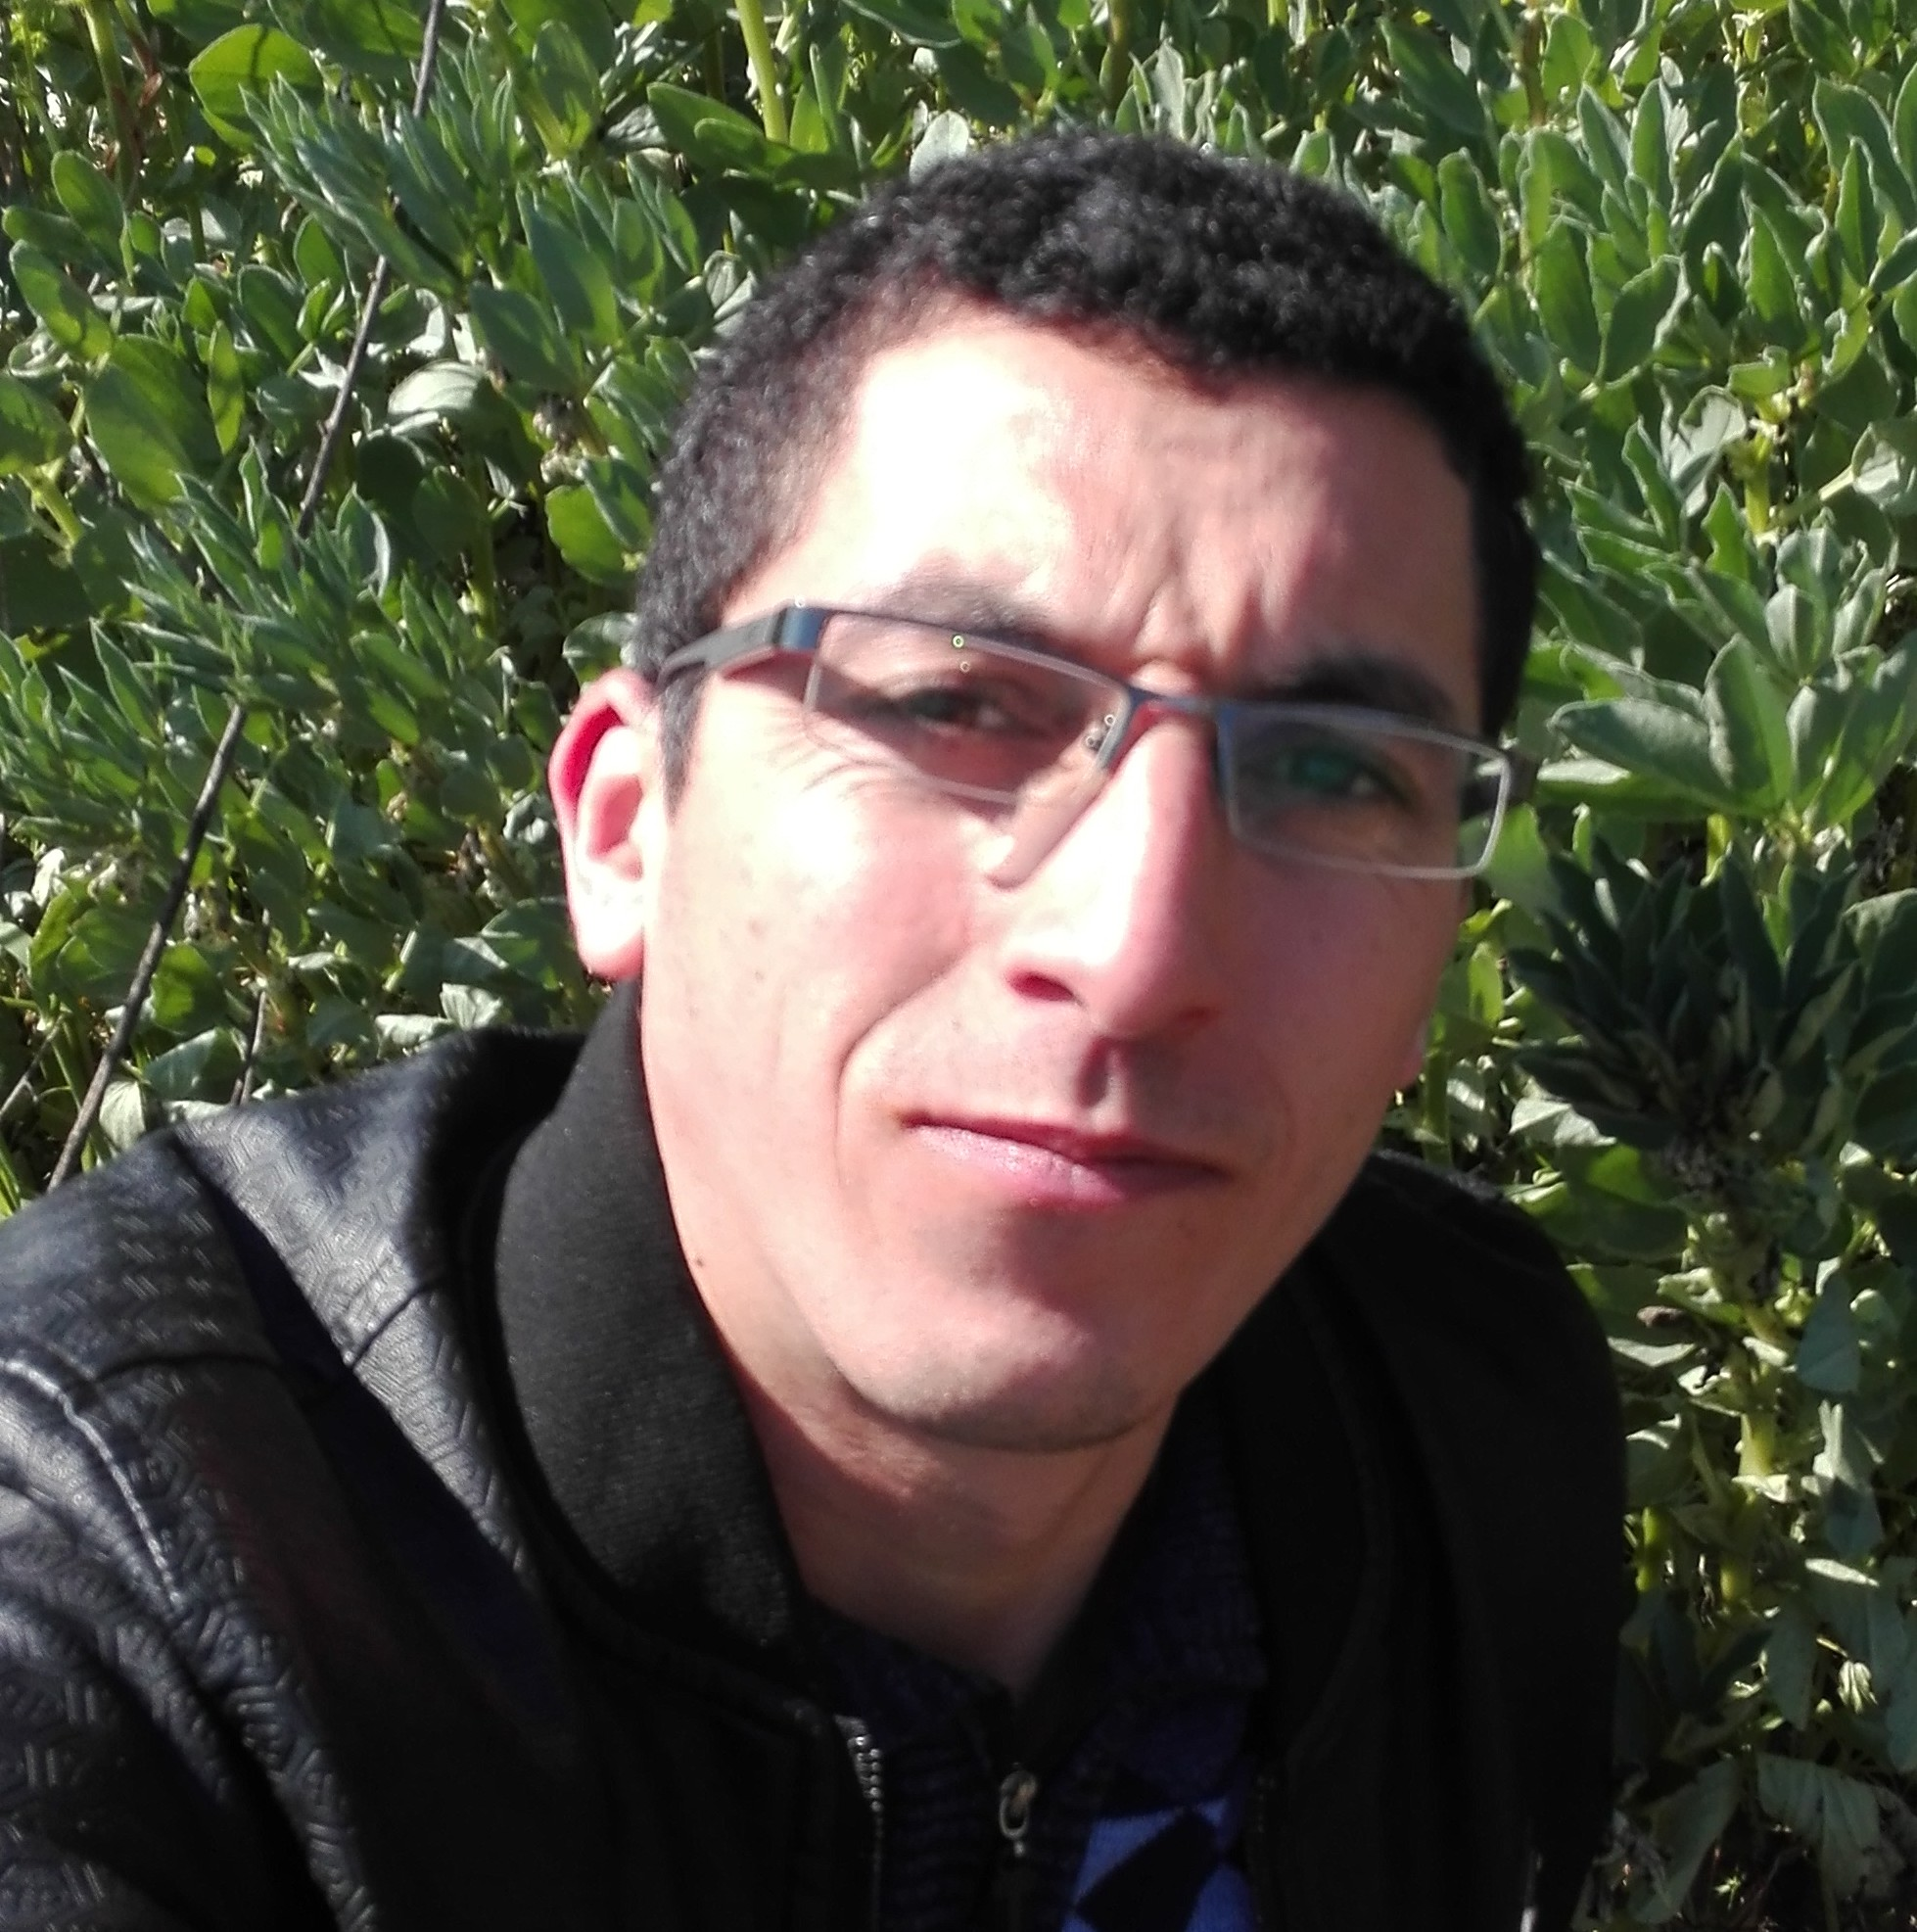
\includegraphics[width=\textwidth]{../img/aak.jpg}
	\end{minipage}
	\begin{minipage}[t]{0.01\textwidth}
	\end{minipage}
	\begin{minipage}[t]{0.80\textwidth}
		\normalsize\vspace*{-0.2\textwidth}
		\textbf{Abdelkrime Aries} has been a lecturer at the National Higher School of Computer Science (ESI), Algiers, since 2013. 
		His main interest lies in artificial intelligence in general and natural language processing in particular. 
		He is passionate about open-source software (\url{https://github.com/kariminf}).
		
		He earned his Ph.D. in Computer Science from ESI in October 2020. 
		He completed his Magister's degree in computer science, specializing in distributed and mobile computing, at ESI in June 2013. 
		The topics of both degrees were related to proposing a method for multilingual automatic summarization. 
		He received his Engineer's degree in computer engineering, specializing in advanced information systems, from the University of Jijel in June 2009. 
		His project focused on developing a system for recognizing Arabic handwritten text using multi-agent architectures.	
	\end{minipage}
	
	
\end{tcolorbox}
%\vspace*{\fill}

\end{document}
